%% abtex2-modelo-trabalho-academico.tex, v-1.9.2 laurocesar
%% Copyright 2012-2014 by abnTeX2 group at http://abntex2.googlecode.com/
%%
%% This work may be distributed and/or modified under the
%% conditions of the LaTeX Project Public License, either version 1.3
%% of this license or (at your option) any later version.
%% The latest version of this license is in
%%   http://www.latex-project.org/lppl.txt
%% and version 1.3 or later is part of all distributions of LaTeX
%% version 2005/12/01 or later.
%%
%% This work has the LPPL maintenance status `maintained'.
%%
%% The Current Maintainer of this work is the abnTeX2 team, led
%% by Lauro César Araujo. Further information are available on
%% http://abntex2.googlecode.com/
%%
%% This work consists of the files abntex2-modelo-trabalho-academico.tex,
%% abntex2-modelo-include-comandos and abntex2-modelo-references.bib
%%

% ------------------------------------------------------------------------
% ------------------------------------------------------------------------
% abnTeX2: Modelo de Trabalho Academico (tese de doutorado, dissertacao de
% mestrado e trabalhos monograficos em geral) em conformidade com
% ABNT NBR 14724:2011: Informacao e documentacao - Trabalhos academicos -
% Apresentacao
% ------------------------------------------------------------------------
% ------------------------------------------------------------------------

%-------------------------------------------------------------------------
% Modelo adaptado especificamente para o contexto do PPgSI-EACH-USP por
% Marcelo Fantinato, com auxílio dos Professores Norton T. Roman, Helton
% H. Bíscaro, e Sarajane M. Peres, em 2016, com muitos agradecimentos aos
% criadores da classe e do modelo base.
%-------------------------------------------------------------------------

\documentclass[
    % -- opções da classe memoir --
    12pt,                % tamanho da fonte
    % openright,            % capítulos começam em pág ímpar (insere página vazia caso preciso)
    oneside,            % para impressão apenas no anverso (apenas frente). Oposto a twoside
    a4paper,            % tamanho do papel.
    % -- opções da classe abntex2 --
    %chapter=TITLE,        % títulos de capítulos convertidos em letras maiúsculas
    %section=TITLE,        % títulos de seções convertidos em letras maiúsculas
    %subsection=TITLE,    % títulos de subseções convertidos em letras maiúsculas
    %subsubsection=TITLE,% títulos de subsubseções convertidos em letras maiúsculas
    % -- opções do pacote babel --
    english,            % idioma adicional para hifenização
    %french,                % idioma adicional para hifenização
    %spanish,            % idioma adicional para hifenização
    brazil                % o último idioma é o principal do documento
    ]{abntex2ppgsi}

% ---
% Pacotes básicos
% ---
% \usepackage{lmodern}            % Usa a fonte Latin Modern
% \usepackage[T1]{fontenc}        % Selecao de codigos de fonte.
\usepackage[utf8]{inputenc}        % Codificacao do documento (conversão automática dos acentos)
\usepackage{lastpage}            % Usado pela Ficha catalográfica
\usepackage{indentfirst}        % Indenta o primeiro parágrafo de cada seção.
\usepackage{color}                % Controle das cores
\usepackage{graphicx}    % Inclusão de gráficos
\usepackage{caption}
\usepackage{subcaption}
\usepackage{microtype}             % para melhorias de justificação
\usepackage{pdfpages}     %para incluir pdf
\usepackage{algpseudocode}            %para ilustrações do tipo algoritmo
\usepackage{mdwlist}            %para itens com espaço padrão da abnt
% \usepackage[noend]{algpseudocode}            %para ilustrações do tipo algoritmo
\usepackage{longtable, multirow}
\usepackage{amsmath,amssymb,amsfonts,amsthm,mathtools}
\usepackage{dsfont}
\usepackage{rotating}
\usepackage{mathrsfs}
% \usepackage{subfig}
% \usepackage{subfigure}


%%% SARA COLOCOU ISSO AQUI - se der problema com numeracao de footnote, tirar isso.
\newcommand\blfootnote[1]{%
  \begingroup
  \renewcommand\thefootnote{}\footnote{#1}%
  \addtocounter{footnote}{-1}%
  \endgroup
}
%%%%%%%%%%%%%%



\DeclareMathOperator*{\argmin}{arg\,min}
\DeclareMathOperator*{\argmax}{arg\,max}
\DeclareMathOperator*{\diag}{diag}
\DeclarePairedDelimiter\abs{\lvert}{\rvert}
\DeclarePairedDelimiter\norm{\lVert}{\rVert}

% Swap the definition of \abs* and \norm*, so that \abs
% and \norm resizes the size of the brackets, and the
% starred version does not.
\makeatletter
\let\oldabs\abs
\def\abs{\@ifstar{\oldabs}{\oldabs*}}
%
\let\oldnorm\norm
\def\norm{\@ifstar{\oldnorm}{\oldnorm*}}
\makeatother

\newcounter{parms} \renewcommand{\theparms}{[\arabic{parms}]}
\newcommand{\newparm}[1]{
  \refstepcounter{parms}\arabic{parms}\label{#1}%
}

\newcommand*{\horzbar}{\rule[.5ex]{2.5ex}{0.5pt}}
\newcommand*{\vertbar}{\rule[-1ex]{0.5pt}{2.5ex}}

\newtheorem{definition}{Definição}
\newtheorem{problem}{Problema}
\newtheorem{theorem}{Teorema}
\newtheorem{corollary}{Corolário}
\newtheorem{proposition}{Proposição}

% \renewcommand\qedsymbol{$\blacksquare$}

% ---
% Pacotes adicionais, usados apenas no âmbito do Modelo Canônico do abnteX2
% ---
\usepackage{lipsum}                % para geração de dummy text
% ---

% ---
% Pacotes de citações
% ---
\usepackage[brazilian,hyperpageref]{backref}     % Paginas com as citações na bibl
\usepackage[alf]{abntex2cite}    % Citações padrão ABNT

% ---
% CONFIGURAÇÕES DE PACOTES
% ---

% ---
% Configurações do pacote backref
% Usado sem a opção hyperpageref de backref
\renewcommand{\backrefpagesname}{Citado na(s) página(s):~}
% Texto padrão antes do número das páginas
\renewcommand{\backref}{}
% Define os textos da citação
\renewcommand*{\backrefalt}[4]{
    \ifcase #1 %
        Nenhuma citação no texto.%
    \or
        Citado na página #2.%
    \else
        Citado #1 vezes nas páginas #2.%
    \fi}%
% ---

% ---
% Informações de dados para CAPA e FOLHA DE ROSTO
% ---

%-------------------------------------------------------------------------
% Comentário adicional do PPgSI - Informações sobre o ``título'':
%
% Em maiúscula apenas a primeira letra da sentença (do título), exceto
% nomes próprios, geográficos, institucionais ou Programas ou Projetos ou
% siglas, os quais podem ter letras em maiúscula também.
%
% O subtítulo do trabalho é opcional.
% Sem ponto final.
%
% Atenção: o título da Dissertação na versão corrigida não pode mudar.
% Ele deve ser idêntico ao da versão original.
%
%-------------------------------------------------------------------------

%\titulo{Fatoração de matrizes no problema de coagrupamento}

%\titulo{Fatoração de matrizes no problema de coagrupamento com sobreposição}

\titulo{Fatoração de matrizes no problema de coagrupamento com sobreposição de colunas}

%\titulo{Fatoração de matrizes no problema de coagrupamento com sobreposição de cogrupos}

%\titulo{Fatoração de matrizes no problema de coagrupamento com sobreposição: Uma aplicação em mineração de textos}

%\titulo{Fatoração de matrizes no problema de coagrupamento com sobreposição de colunas: Uma aplicação em mineração de textos}

%-------------------------------------------------------------------------
% Comentário adicional do PPgSI - Informações sobre o ``autor'':
%
% Todas as letras em maiúsculas.
% Nome completo.
% Sem ponto final.
%-------------------------------------------------------------------------
\autor{\uppercase{Lucas Fernandes Brunialti}}

%-------------------------------------------------------------------------
% Comentário adicional do PPgSI - Informações sobre o ``local'':
%
% Não incluir o ``estado''.
% Sem ponto final.
%-------------------------------------------------------------------------
\local{São Paulo}

%-------------------------------------------------------------------------
% Comentário adicional do PPgSI - Informações sobre a ``data'':
%
% Colocar o ano do depósito (ou seja, o ano da entrega) da respectiva
% versão, seja ela a versão original (para a defesa) seja ela a versão
% corrigida (depois da aprovação na defesa).
%
% Atenção: Se a versão original for depositada no final do ano e a versão
% corrigida for entregue no ano seguinte, o ano precisa ser atualizado no
% caso da versão corrigida.
% Cuidado, pois o ano da ``capa externa'' também precisa ser atualizado
% nesse caso.
%
% Não incluir o dia, nem o mês.
% Sem ponto final.
%-------------------------------------------------------------------------
\data{2016}

%-------------------------------------------------------------------------
% Comentário adicional do PPgSI - Informações sobre o ``Orientador'':
%
% Se for uma professora, trocar por ``Profa. Dra.''
% Nome completo.
% Sem ponto final.
%-------------------------------------------------------------------------
\orientador{Profa. Dra. Sarajane Marques Peres}

%-------------------------------------------------------------------------
% Comentário adicional do PPgSI - Informações sobre o ``Coorientador'':
%
% Opcional. Incluir apenas se houver co-orientador formal, de acordo com o
% Regulamento do Programa.
%
% Se for uma professora, trocar por ``Profa. Dra.''
% Nome completo.
% Sem ponto final.
%-------------------------------------------------------------------------
%\coorientador{Prof. Dr. Valdinei Freire Silva}

\tipotrabalho{Dissertação (Mestrado)}

\preambulo{
%-------------------------------------------------------------------------
% Comentário adicional do PPgSI - Informações sobre o texto ``Versão
% original'':
%
% Não usar para Qualificação.
% Não usar para versão corrigida de Dissertação.
%
%-------------------------------------------------------------------------
Versão original
%-------------------------------------------------------------------------
% Comentário adicional do PPgSI - Informações sobre o ``texto principal do
% preambulo'':
%
% Para Qualificação, trocar por: Texto de Exame de Qualificação apresentado à Escola de Artes, Ciências e Humanidades da Universidade de São Paulo como parte dos requisitos para obtenção do título de Mestre em Ciências pelo Programa de Pós-graduação em Sistemas de Informação.
%
%-------------------------------------------------------------------------
\newline \newline \newline Dissertação apresentada à Escola de Artes, Ciências e Humanidades da Universidade de São Paulo para obtenção do título de Mestre em Ciências pelo Programa de Pós-graduação em Sistemas de Informação.
%
\newline \newline Área de concentração: Metodologia e Técnicas da Computação
%-------------------------------------------------------------------------
% Comentário adicional do PPgSI - Informações sobre o texto da ``Versão
% corrigida'':
%
% Não usar para Qualificação.
% Não usar para versão original de Dissertação.
%
% Substituir ``xx de xxxxxxxxxxxxxxx de xxxx'' pela ``data da defesa''.
%
%-------------------------------------------------------------------------
%\newline \newline \newline Versão corrigida contendo as alterações solicitadas pela comissão julgadora em xx de xxxxxxxxxxxxxxx de xxxx. A versão original encontra-se em acervo reservado na Biblioteca da EACH-USP e na Biblioteca Digital de Teses e Dissertações da USP (BDTD), de acordo com a Resolução CoPGr 6018, de 13 de outubro de 2011.
}
% ---


% ---
% Configurações de aparência do PDF final

% alterando o aspecto da cor azul
\definecolor{blue}{RGB}{41,5,195}

% informações do PDF
\makeatletter
\hypersetup{
         %pagebackref=true,
        pdftitle={\@title},
        pdfauthor={\@author},
        pdfsubject={\imprimirpreambulo},
        pdfcreator={LaTeX com abnTeX2 adaptado para o PPgSI-EACH-USP},
        pdfkeywords={abnt}{latex}{abntex}{abntex2}{qualificação de mestrado}{dissertação de mestrado}{ppgsi},
        colorlinks=true,               % false: boxed links; true: colored links
        linkcolor=blue,              % color of internal links
        citecolor=blue,                % color of links to bibliography
        filecolor=magenta,              % color of file links
        urlcolor=blue,
        bookmarksdepth=4
}
\makeatother
% ---

% ---
% Espaçamentos entre linhas e parágrafos
% ---

% O tamanho do parágrafo é dado por:
\setlength{\parindent}{1.25cm}

% Controle do espaçamento entre um parágrafo e outro:
\setlength{\parskip}{0cm}  % tente também \onelineskip
\renewcommand{\baselinestretch}{1.5}

% ---
% compila o indice
% ---
\makeindex
% ---

    % Controlar linhas orfas e viuvas
  \clubpenalty10000
  \widowpenalty10000
  \displaywidowpenalty10000

% ----
% Início do documento
% ----
\begin{document}

% Retira espaço extra obsoleto entre as frases.
\frenchspacing

% ----------------------------------------------------------
% ELEMENTOS PRÉ-TEXTUAIS
% ----------------------------------------------------------
% \pretextual

% ---
% Capa
% ---
%-------------------------------------------------------------------------
% Comentário adicional do PPgSI - Informações sobre a ``capa'':
%
% Esta é a ``capa'' principal/oficial do trabalho, a ser impressa apenas
% para os casos de encadernação simples (ou seja, em ``espiral'' com
% plástico na frente).
%
% Não imprimir esta ``capa'' quando houver ``capa dura'' ou ``capa brochura''
% em que estas mesmas informações já estão presentes nela.
%
%-------------------------------------------------------------------------
\imprimircapa
% ---

% ---
% Folha de rosto
% (o * indica que haverá a ficha bibliográfica)
% ---
\imprimirfolhaderosto*
% ---

% ---
% Inserir a autorização para reprodução e ficha bibliografica
% ---

%-------------------------------------------------------------------------
% Comentário adicional do PPgSI - Informações sobre o texto da
% ``autorização para reprodução e ficha bibliografica'':
%
% Página a ser usada apenas para Dissertação (tanto na versão original
% quanto na versão corrigida).
%
% Solicitar a ficha catalográfica na Biblioteca da EACH.
% Duas versões devem ser solicitadas, em dois momentos distintos: uma vez
% para a versão original, e depois outra atualizada para a corrigida.
%
% Atenção: esta página de ``autorização para reprodução e ficha
% catalográfica'' deve ser impressa obrigatoriamente no verso da folha de
% rosto.
%
% Não usar esta página para Qualificação.
%
% Substitua o arquivo ``fig_ficha_catalografica.pdf'' abaixo referenciado
% pelo PDF elaborado pela Biblioteca
%
%-------------------------------------------------------------------------
\begin{fichacatalografica}
    
\includepdf{fig_ficha_catalografica.pdf}
\end{fichacatalografica}

% ---
% Inserir errata
% ---
%-------------------------------------------------------------------------
% Comentário adicional do PPgSI - Informações sobre ``Errata'':
%
% Usar esta página de errata apenas em casos de excepcionais, e apenas
% para a versão corrigida da Dissertação. Por exemplo, quando depois de
% já depositada e publicada a versão corrigida, ainda assim verifica-se
% a necessidade de alguma correção adicional.
%
% Se precisar usar esta página, busque a forma correta (o modelo correto)
% para fazê-lo, de acordo com a norma ABNT.
%
% Não usar esta página para versão original de Dissertação.
% Não usar esta página para Qualificação.
%
%-------------------------------------------------------------------------
%\begin{errata}
%Elemento opcional para versão corrigida, depois de depositada.
%\end{errata}
% ---

% ---
% Inserir folha de aprovação
% ---

\begin{folhadeaprovacao}
%-------------------------------------------------------------------------
% Comentário adicional do PPgSI - Informações sobre ``Folha da aprovação'':
%
% Para Qualificação, trocar por: Texto de Exame de Qualificação de autoria de Fulano de Tal, sob o título \textbf{``\imprimirtitulo''}, apresentado à Escola de Artes, Ciências e Humanidades da Universidade de São Paulo, como parte dos requisitos para obtenção do título de Mestre em Ciências pelo Programa de Pós-graduação em Sistemas de Informação, na área de concentração Sistemas de Informação, aprovado em \_\_\_ de \_\_\_\_\_\_\_\_\_\_\_\_\_\_ de \_\_\_\_\_\_ pela comissão examinadora constituída pelos doutores:
%
% Substituir ``Fulano de Tal'' pelo nome completo do autor do trabalho, com
% apenas as iniciais em maiúsculo.
%
% Substiuir ``___ de ______________ de ______'' por:
%     - Para versão original de Dissertação: deixar em branco, pois a data
%       pode mudar, mesmo que ela já esteja prevista.
%     - Para versão corrigida de Dissertação: usar a data em que a defesa
%       efetivamente ocorreu.
%
%-------------------------------------------------------------------------
\noindent Dissertação de autoria de Lucas Fernandes Brunialti, sob o título \textbf{\imprimirtitulo}, apresentada à Escola de Artes, Ciências e Humanidades da Universidade de São Paulo, para obtenção do título de Mestre em Ciências pelo Programa de Pós-graduação em Sistemas de Informação, na área de concentração Sistemas de Informação, aprovada em \_\_\_ de \_\_\_\_\_\_\_\_\_\_\_\_\_\_ de \_\_\_\_\_\_ pela comissão julgadora constituída pelos doutores:

\vspace*{3cm}

\begin{center}
%-------------------------------------------------------------------------
% Comentário adicional do PPgSI - Informações sobre ``assinaturas'':
%
% Para Qualificação e para versão original de Dissertação: deixar em
% branco (ou seja, assim como está abaixo), pois os membros da banca podem
% mudar, mesmo que eles já estejam previstos.
%
% Para versão corrigida de Dissertação: usar os dados dos examinadores que
% efetivamente participaram da defesa.
%
% Em nenhum caso há realmente necessidade de assinaturas.
%
% Para versão corrigida de Dissertação: em caso de ``professora'', trocar
% por ``Profa. Dra.''
%
% Para versão corrigida de Dissertação: ao colocar os nomes dos
% examinadores, remover o sublinhado
%
% Para versão corrigida de Dissertação: ao colocar os nomes dos
% examinadores, usar seus nomes completos, exatamente conforme constam em
% seus Currículos Lattes
%
% Para versão corrigida de Dissertação: ao colocar os nomes das
% instituições, remover o sublinhado e remover a palavra ``Instituição:''
%
% Não abreviar os nomes das instituições.
%
%-------------------------------------------------------------------------
\textbf{Prof. Dr. \_\_\_\_\_\_\_\_\_\_\_\_\_\_\_\_\_\_\_\_\_}
\\ Presidente
\\ Instituição: \_\_\_\_\_\_\_\_\_\_\_\_\_\_\_\_\_\_\_\_\_

\vspace*{2cm}

\textbf{Prof. Dr. \_\_\_\_\_\_\_\_\_\_\_\_\_\_\_\_\_\_}
\\ Instituição: \_\_\_\_\_\_\_\_\_\_\_\_\_\_\_\_\_\_\_

\vspace*{2cm}

\textbf{Prof. Dr. \_\_\_\_\_\_\_\_\_\_\_\_\_\_\_\_\_\_}
\\ Instituição: \_\_\_\_\_\_\_\_\_\_\_\_\_\_\_\_\_\_\_

\end{center}

\end{folhadeaprovacao}
% ---

% ---
% Dedicatória
% ---
%-------------------------------------------------------------------------
% Comentário adicional do PPgSI - Informações sobre ``Dedicatória'':
%
% Opcional para Dissertação.
% Não sugerido para Qualificação.
%
%-------------------------------------------------------------------------
\begin{dedicatoria}
   \vspace*{\fill}
   \centering
   \noindent
   \textit{À minha noiva Beatriz, aos meus pais Sandra e Ronaldo, aos meus orientadores Sarajane e Valdinei, e aos amigos e empresas que me apoiaram nesses três anos}
     \vspace*{\fill}
\end{dedicatoria}
% ---

% ---
% Agradecimentos
% ---
%-------------------------------------------------------------------------
% Comentário adicional do PPgSI - Informações sobre ``Agradecimentos'':
%
% Opcional para Dissertação.
% Não sugerido para Qualificação.
%
% Lembrar de agradecer agências de fomento e outras instituições similares.
%
%-------------------------------------------------------------------------
% \begin{agradecimentos}
% Texto de exemplo, texto de exemplo, texto de exemplo, texto de exemplo, texto de exemplo, texto de exemplo, texto de exemplo, texto de exemplo, texto de exemplo, texto de exemplo, texto de exemplo, texto de exemplo, texto de exemplo, texto de exemplo, texto de exemplo, texto de exemplo, texto de exemplo, texto de exemplo, texto de exemplo, texto de exemplo, texto de exemplo, texto de exemplo.

% Texto de exemplo, texto de exemplo, texto de exemplo, texto de exemplo, texto de exemplo, texto de exemplo, texto de exemplo, texto de exemplo, texto de exemplo, texto de exemplo, texto de exemplo, texto de exemplo, texto de exemplo, texto de exemplo, texto de exemplo, texto de exemplo, texto de exemplo, texto de exemplo, texto de exemplo, texto de exemplo, texto de exemplo, texto de exemplo.

% Texto de exemplo, texto de exemplo, texto de exemplo, texto de exemplo, texto de exemplo, texto de exemplo, texto de exemplo, texto de exemplo, texto de exemplo, texto de exemplo, texto de exemplo, texto de exemplo, texto de exemplo, texto de exemplo, texto de exemplo, texto de exemplo, texto de exemplo, texto de exemplo, texto de exemplo, texto de exemplo, texto de exemplo, texto de exemplo.

% Texto de exemplo, texto de exemplo, texto de exemplo, texto de exemplo, texto de exemplo, texto de exemplo, texto de exemplo, texto de exemplo, texto de exemplo, texto de exemplo, texto de exemplo, texto de exemplo, texto de exemplo, texto de exemplo, texto de exemplo, texto de exemplo, texto de exemplo, texto de exemplo, texto de exemplo, texto de exemplo, texto de exemplo, texto de exemplo.

% Texto de exemplo, texto de exemplo, texto de exemplo, texto de exemplo, texto de exemplo, texto de exemplo, texto de exemplo, texto de exemplo, texto de exemplo, texto de exemplo, texto de exemplo, texto de exemplo, texto de exemplo, texto de exemplo, texto de exemplo, texto de exemplo, texto de exemplo, texto de exemplo, texto de exemplo, texto de exemplo, texto de exemplo, texto de exemplo.
% \end{agradecimentos}
% ---

% ---
% Epígrafe
% ---
%-------------------------------------------------------------------------
% Comentário adicional do PPgSI - Informações sobre ``Epígrafe'':
%
% Opcional para Dissertação.
% Não sugerido para Qualificação.
%
%-------------------------------------------------------------------------
% \begin{epigrafe}
%     \vspace*{\fill}
%     \begin{flushright}
%         \textit{``Escreva aqui uma epígrafe, se desejar, ou remova esta página...''\\
%         (Autor da epígrafe)}
%     \end{flushright}
% \end{epigrafe}
% ---

% ---
% RESUMOS
% ---

% resumo em português
\setlength{\absparsep}{18pt} % ajusta o espaçamento dos parágrafos do resumo
\begin{resumo}

%-------------------------------------------------------------------------
% Comentário adicional do PPgSI - Informações sobre ``referência'':
%
% Troque os seguintes campos pelos dados de sua Dissertação (mantendo a
% formatação e pontuação):
%   - SOBRENOME
%   - Nome1
%   - Nome2
%   - Nome3
%   - Título do trabalho: subtítulo do trabalho
%   - AnoDeDefesa
%
% Mantenha todas as demais informações exatamente como estão.
%
% [Não usar essas informações de ``referência'' para Qualificação]
%
%-------------------------------------------------------------------------
\begin{flushleft}
BRUNIALTI, Lucas Fernandes. \textbf{Fatoração de matrizes no problema de coagrupamento com sobreposição de colunas}. \imprimirdata. \pageref{LastPage} f. Dissertação (Mestrado em Ciências) – Escola de Artes, Ciências e Humanidades, Universidade de São Paulo, São Paulo, 2016.
\end{flushleft}

Coagrupamento é uma estratégia para análise de dados capaz de encontrar grupos de dados, então denominados cogrupos, que são formados considerando subconjuntos diferentes das  características descritivas dos dados.
Contextos de aplicação caracterizados por apresentar subjetividade, como mineração de texto, são candidatos a serem submetidos à estratégia de coagrupamento; a flexibilidade em associar textos de acordo com características parciais representa um tratamento adequado à tal subjetividade.
Um método para implementação de coagrupamento capaz de lidar com esse tipo de dados é a fatoração de matrizes.
Nesta dissertação de mestrado são propostas duas estratégias para coagrupamento baseadas em fatoração de matrizes não-negativas, capazes de encontrar cogrupos organizados com sobreposição de colunas em uma matriz de valores reais positivos.
As estratégias são apresentadas em termos de suas definições formais e seus algoritmos para implementação.
Resultados experimentais quantitativos e qualitativos são fornecidos a partir de problemas baseados em conjuntos de dados sintéticos e em conjuntos de dados reais, sendo esses últimos contextualizados na área de mineração de texto.
Os resultados são analisados em termos de quantização do espaço e capacidade de reconstrução, capacidade de agrupamento utilizando as métricas índice de Rand e informação mútua normalizada e geração de informação (interpretabilidade dos modelos).
Os resultados confirmam a hipótese de que as estratégias propostas são capazes de descobrir cogrupos com sobreposição de forma natural, e que tal organização de cogrupos fornece informação detalhada, e portanto de valor diferenciado, para as áreas de análise de agrupamento e mineração de texto.

Palavras-chaves: Coagrupamento. Fatoração de Matrizes Não-negativas. Análise de Agrupamento. Mineração de Texto.
\end{resumo}

% resumo em inglês
%-------------------------------------------------------------------------
% Comentário adicional do PPgSI - Informações sobre ``resumo em inglês''
%
% Caso a Qualificação ou a Dissertação inteira seja elaborada no idioma inglês,
% então o ``Abstract'' vem antes do ``Resumo''.
%
%-------------------------------------------------------------------------
\begin{resumo}[Abstract]
\begin{otherlanguage*}{english}

%-------------------------------------------------------------------------
% Comentário adicional do PPgSI - Informações sobre ``referência em inglês''
%
% Troque os seguintes campos pelos dados de sua Dissertação (mantendo a
% formatação e pontuação):
%     - SURNAME
%     - FirstName1
%     - MiddleName1
%     - MiddleName2
%     - Work title: work subtitle
%     - DefenseYear (Ano de Defesa)
%
% Mantenha todas as demais informações exatamente como estão.
%
% [Não usar essas informações de ``referência'' para Qualificação]
%
%-------------------------------------------------------------------------
\begin{flushleft}
BRUNIALTI, Lucas Fernandes. \textbf{Matrix factorization for overlapping columns coclustering}. \imprimirdata. \pageref{LastPage} p. Dissertation (Master of Science) – School of Arts, Sciences and Humanities, University of São Paulo, São Paulo, 2016.
\end{flushleft}

Coclustering is a data analysis strategy which is able to discover data clusters, known as coclusters.
This technique allows data to be clustered based on different subsets defined by data descriptive features.
Application contexts characterized by subjectivity, such as text mining, are applicable candidates for applying coclustering strategy due to the flexibility to associate documents according to partial features.
The coclustering method can be implemented by means of matrix factorization, which is suitable to handle this type of data.
In this thesis two strategies are proposed in non-negative matrix factorization for coclustering.
These strategies are able to find column overlapping coclusters in a given dataset of positive data and are presented in terms of their formal definitions as well as their algorithms' implementation.
Quantitative and qualitative experimental results are presented through applying synthetic datasets and real datasets contextualized in text mining.
This is accomplished by analyzing them in terms of space quantization, clustering capabilities and generated information (interpretability of models).
The well known external metrics Rand index and normalized mutual information are used to achieve the analysis of clustering capabilities.
Results confirm the hypothesis that the proposed strategies are able to discover overlapping coclusters naturally.
Moreover, these coclusters produced by the new algorithms provide detailed information and are thus valuable for future research in cluster analysis and text mining.

Keywords: Coclustering. Non-negative Matrix Factorization. Cluster Analysis. Text Mining.
\end{otherlanguage*}
\end{resumo}

% ---
% ---
% inserir lista de figuras
% ---
\pdfbookmark[0]{\listfigurename}{lof}
\addtocontents{toc}{\protect\sloppy}
\listoffigures*
\cleardoublepage
% ---

% ---
% inserir lista de algoritmos
% ---
\pdfbookmark[0]{\listalgorithmname}{loa}
\listofalgorithms
\cleardoublepage

% ---
% inserir lista de tabelas
% ---
\pdfbookmark[0]{\listtablename}{lot}
\listoftables*
\cleardoublepage
% ---

% ---
% inserir lista de abreviaturas e siglas
% ---
%-------------------------------------------------------------------------
% Comentário adicional do PPgSI - Informações sobre ``Lista de abreviaturas
% e siglas'':
%
% Opcional.
% Uma vez que se deseja usar, é necessário manter padrão e consistência no
% trabalho inteiro.
% Se usar: inserir em ordem alfabética.
%
%-------------------------------------------------------------------------
% \begin{siglas}
%   \item[Sigla/abreviatura 1] Definição da sigla ou da abreviatura por extenso
%   \item[Sigla/abreviatura 2] Definição da sigla ou da abreviatura por extenso
%   \item[Sigla/abreviatura 3] Definição da sigla ou da abreviatura por extenso
%   \item[Sigla/abreviatura 4] Definição da sigla ou da abreviatura por extenso
%   \item[Sigla/abreviatura 5] Definição da sigla ou da abreviatura por extenso
%   \item[Sigla/abreviatura 6] Definição da sigla ou da abreviatura por extenso
%   \item[Sigla/abreviatura 7] Definição da sigla ou da abreviatura por extenso
%   \item[Sigla/abreviatura 8] Definição da sigla ou da abreviatura por extenso
%   \item[Sigla/abreviatura 9] Definição da sigla ou da abreviatura por extenso
%   \item[Sigla/abreviatura 10] Definição da sigla ou da abreviatura por extenso
% \end{siglas}
% ---

% ---
% inserir lista de símbolos
% ---
%-------------------------------------------------------------------------
% Comentário adicional do PPgSI - Informações sobre ``Lista de símbolos'':
%
% Opcional.
% Uma vez que se deseja usar, é necessário manter padrão e consistência no
% trabalho inteiro.
% Se usar: inserir na ordem em que aparece no texto.
%
%-------------------------------------------------------------------------
% \begin{simbolos}
%   \item[$ \Gamma $] Letra grega Gama
%   \item[$ \Lambda $] Lambda
%   \item[$ \zeta $] Letra grega minúscula zeta
%   \item[$ \in $] Pertence
% \end{simbolos}
% ---

% ---
% inserir o sumario
% ---
% \pdfbookmark[0]{\contentsname}{toc}
% \tableofcontents*
% \cleardoublepage

\pdfbookmark[0]{\contentsname}{toc}
\addtocontents{toc}{\protect\sloppy}
\tableofcontents*
\cleardoublepage
% ---



% ----------------------------------------------------------
% ELEMENTOS TEXTUAIS
% ----------------------------------------------------------
\textual



%-------------------------------------------------------------------------
% Comentário adicional do PPgSI - Informações sobre ``títulos de seções''
%
% Para todos os títulos (seções, subseções, tabelas, ilustrações, etc):
%
% Em maiúscula apenas a primeira letra da sentença (do título), exceto
% nomes próprios, geográficos, institucionais ou Programas ou Projetos ou
% siglas, os quais podem ter letras em maiúscula também.
%
%-------------------------------------------------------------------------

% Example of table
% \begin{table}[htbp]
%     \centering
%     \caption{Exemplo de título de tabela}
%         \begin{tabular}{p{1in} p{1in} p{1in} p{1in} } \hline

%         Cabeçalho 1    & Cabeçalho 2    & Cabeçalho 3    & Cabeçalho 4 \\ \hline
%         Texto    & número & número    & número \\
%         Texto    & número & número    & número \\
%         Texto    & número & número    & número \\
%         Texto    & número & número    & número \\
%         Texto    & número & número    & número \\ \hline

%         \end{tabular}
%     \label{tab:ExemploDeTabela1}
%   \source{Marcelo Fantinato, 2016}
% \end{table}

\chapter{Introdução}
\label{cap:intro}

% Não há padronização nas representações para as melhores representações.
% - Não colocar que uma representação é melhor que a outra
% - Conclusao:
%     * pensei nos algos, qual contribuição:
%        - entender os algoritmos originais
%        - propor mudança de concepcao no modelo
%        - verificar se isso era possivel
%        - teste empirico
%        - derivação
%        - experimentacao onde percebo algos, destaque especifico para os algoritmos BinOvNMTF
%        - Hipotese: pq eles se destacam

% Introducao:
%     - como os algos da literatura tratam sobreposicao
%     - estudando quantizacao, etc (final cap 3 e 5)


Segundo~\citeonline{Jain1999}, a análise de agrupamento pode ser vista como uma tarefa exploratória que tem o objetivo de organizar uma coleção de dados em um conjunto de grupos, segundo a similaridade ou dissimilaridade existente entre esses dados.
Tradicionalmente, os métodos usados para análise de agrupamento são desenvolvidos para minimizar a similaridade intragrupos e maximizar a similaridade intergrupos; e precisam encontrar uma organização ``natural'' em grupos que acomode cada dado do conjunto sob análise em um grupo específico.

Estratégias de diferentes naturezas -- particional, hierárquica, baseada em densidade, etc~\cite{Han2011,Xu2005} -- podem ser usadas para alcançar o objetivo da análise de agrupamento, e cada uma delas possui características que as fazem mais ou menos suscetíveis para conjuntos de dados de diferentes naturezas.
Ainda, sob o contexto clássico da tarefa de agrupamento, os métodos precisam lidar com a similaridade entre os dados tomando como base a comparação de todas as suas características descritivas e, de alguma forma, precisam ser capazes de descobrir quais características de fato tornam dados em um grupo de dados mais similares entre si.

Ao longo do tempo, pesquisadores da área de análise de agrupamento vêm propondo flexibilizações na definição da tarefa de agrupamento de forma a adequá-la a contextos mais realísticos, nos quais a organização natural dos dados em um conjunto de dados não pressupõe restrições como a pertinência de um dado a um único grupo ou a possibilidade de agrupar dados de acordo com similaridades em subconjuntos de atributos descritivos~\cite{Bezdek1981,Han2011,Peres2012}.
Essa forma de tratar a tarefa de agrupamento permite melhorias no processo de descoberta de agrupamentos sob dois aspectos: facilita o trabalho do método que busca os grupos, pois flexibiliza a maneira como os atributos descritivos dos dados, ou a pertinência do dado aos grupos, influencia no processo de agrupamento; fornece um conjunto de informações diferenciado, permitindo que análises mais refinadas sejam realizadas na interpretação dos grupos apresentados como resultado.

Esse diferencial pode ser especialmente útil quando o contexto da aplicação da análise de agrupamento apresenta alguma subjetividade em termos de interpretação de resultados, um fato bastante comum em tarefas de mineração de texto, por exemplo.
Considere um contexto de uma aplicação de mineração de texto em que o objetivo é encontrar notícias similares à uma notícia fornecida como entrada, seja para recomendação, aumentando o engajamento de usuários em um portal de notícias, ou até mesmo para descoberta de conhecimento, a fim de ajudar na tomada de decisões de negócio nesse portal de notícias, por exemplo.
A análise de agrupamento com base na similaridade que considera todos os atributos (palavras), em um conjunto de notícias que representam os temas esportes (colunas \#1, \#2 e \#3 na figura~\ref{fig:sistema:a}) e música (colunas \#4, \#5 e \#6 na figura~\ref{fig:sistema:a}), seria capaz de particionar as notícias em dois grupos, que representariam esses dois temas.
Embora essas recomendações pareçam ser ideais, e sob algum aspecto de análise elas são, é factível assumir que essa análise de agrupamento é prática, mas talvez menos útil e interessante do que poderia ser.

Uma possibilidade de melhoria dessa aplicação hipotética seria usar um algoritmo de análise de agrupamento que permitisse descobrir uma organização de grupos de notícias baseada em similaridades parciais ou baseada em partes~\cite{Franca2010,Ho2008}.
Assim, seria possível encontrar grupos que não são encontrados quando se considera todas as características na análise de agrupamento.

Considerando tal possibilidade, a aplicação seria dotada da capacidade de perceber, por exemplo, que algumas notícias podem trazer conteúdo referente a diferentes contextos se forem analisadas apenas sob determinados aspectos.
Nesse caso, os grupos formados durante a análise de agrupamento seriam capazes de refletir a diversidade de contextos abordados em uma notícia, fazendo-a pertencer a diferentes grupos, por diferentes motivos.
Por exemplo, é sabido que eventos de beisebol -- o \textit{superbowl} -- possuem uma abertura cultural na qual grandes artistas da música fazem apresentações; ou eventos de esportes radicais, como tirolesa, acontecem em eventos de música contemporâneos -- \textit{rock in rio}.
Tais notícias deveriam aparecer em grupos caracterizados por notícias referentes à esportes, notícias referentes à música, ou notícias referentes à esporte e música (Figuras~\ref{fig:sistema:b} e~\ref{fig:sistema:c}).

\begin{figure} [htpb]
\centering
 \caption{
        Representação de uma aplicação de mineração de dados implementada a partir de análise de agrupamento com similaridade total (a) e similaridade parcial (b,c). Os grupos são diferenciados por cores.
    }
    \begin{subfigure}[b]{0.45\textwidth}
        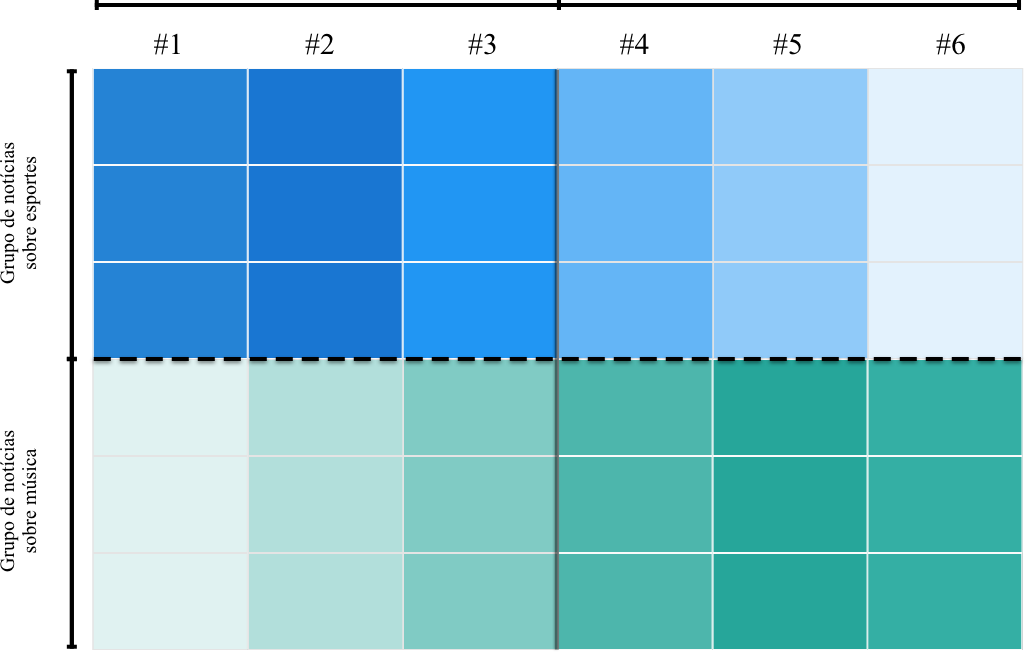
\includegraphics[width=\textwidth]{img/sistema0.png}
        \caption{}
        \label{fig:sistema:a}
    \end{subfigure}
    ~
    \begin{subfigure}[b]{0.45\textwidth}
        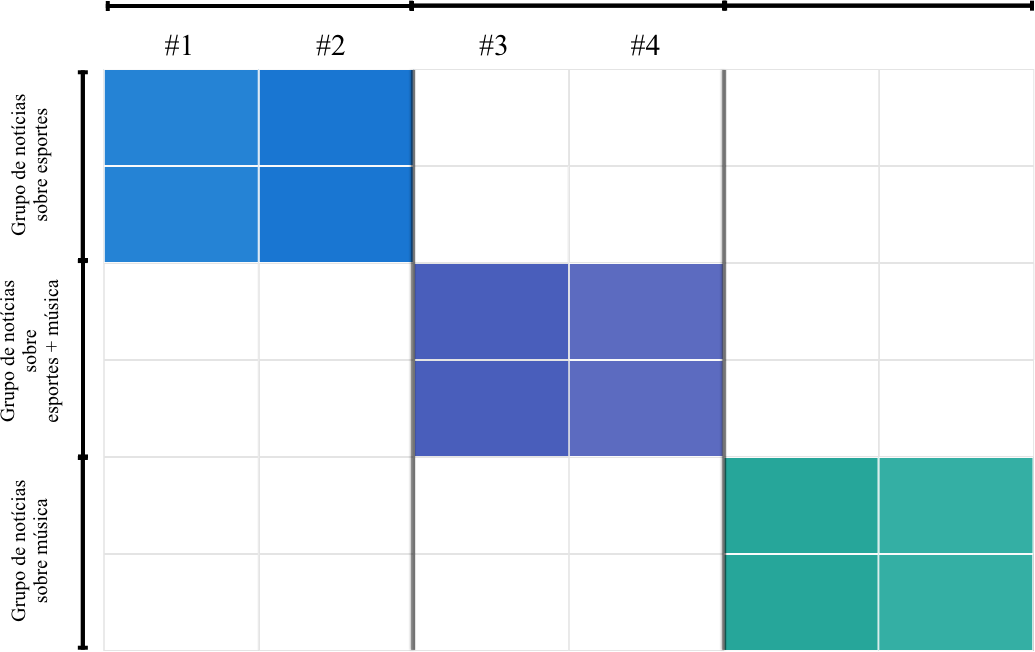
\includegraphics[width=\textwidth]{img/sistema1.png}
        \caption{}
        \label{fig:sistema:b}
    \end{subfigure}
    ~
    \begin{subfigure}[b]{0.45\textwidth}
        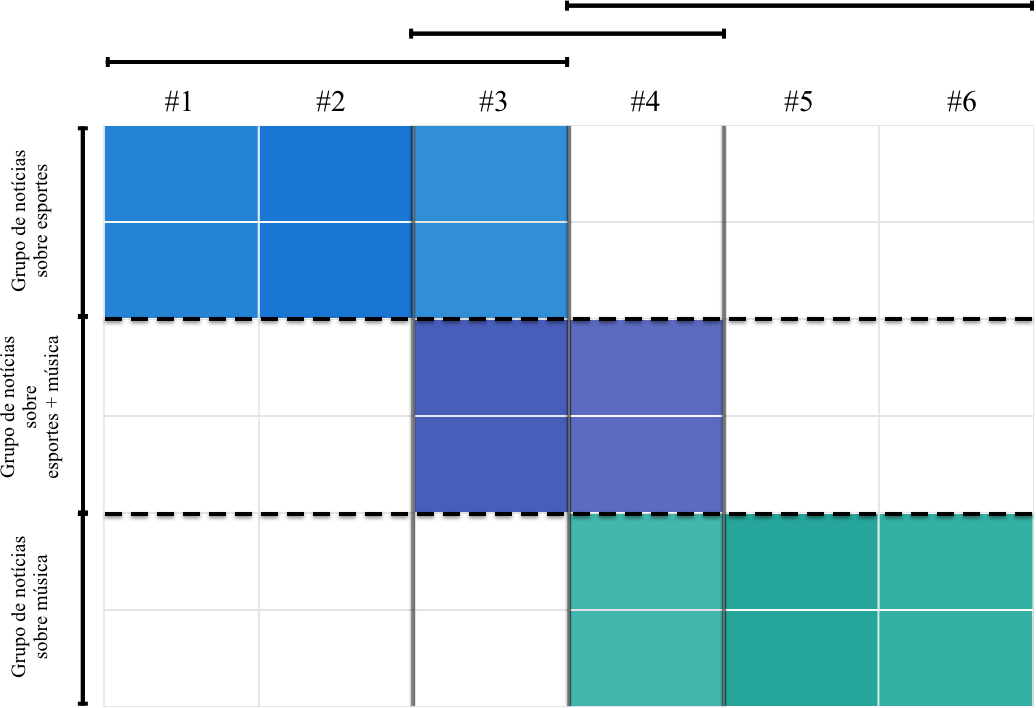
\includegraphics[width=\textwidth]{img/sistema2.png}
        \caption{}
        \label{fig:sistema:c}
    \end{subfigure}
    \source{Lucas Fernandes Brunialti, 2016}
\end{figure}

Nas figuras~\ref{fig:sistema:b} e~\ref{fig:sistema:c} é introduzido graficamente o conceito de coagrupamento.
Nesse contexto, o problema de mineração de texto é modelado como o problema de encontrar uma organização dos textos em grupos considerando similaridades parciais.
Assim, um texto pode pertencer a um ou mais cogrupos, a depender dos atributos descritivos sendo considerados.

Portanto, nessa aplicação, uma análise de agrupamento com maior capacidade de extração de informação e interpretabilidade, consideraria que o grupo de notícias referentes aos assuntos esportes e música tem sobreposição nas palavras que formam o grupo de notícias sobre música e o grupo de notícias sobre esportes (Figura~\ref{fig:sistema:c}).

A nomenclatura coagrupamento deriva da estratégia de análise de dados executada durante o processo de descoberta de grupos.
Nesse caso, tanto os dados (linhas) quanto os seus atributos descritivos (colunas) são mutuamente submetidos a uma análise de similaridade, e portanto, grupos de dados (linhas) são estabelecidos com respeito a grupos de atributos (colunas), e grupos de atributos (colunas) também são estabelecidos com respeito a grupos de dados (linhas).

A associação da análise de coagrupamentos a mineração de texto é interessante pois essa tarefa constitui-se como um problema no qual é preciso lidar com a necessidade de apresentação de resultados que geram informações passíveis de serem interpretadas.
Esse problema pode ser bem resolvido com a estratégia de coagrupamento pois os grupos de atributos que são gerados por ela podem revelar informação antes escondida nos dados~\cite{Tjhi2009}, e que em um processo de agrupamento tradicional não poderiam ser, pelo menos diretamente, descobertas.

Dentre os diferentes métodos existentes na literatura, referentes à implementação de análise de coagrupamento~\cite{Franca2010,Mirkin1996,Madeira2004}, os métodos que usam fatoração de matrizes não-negativas~\cite{lee:nnmf00,lee99} têm sido vistos como uma boa alternativa a ser aplicada no contexto de mineração de texto, dado que esses métodos têm vantagens para lidar com dados representados como matrizes positivas~\cite{Xu2003,Shahnaz2006373,Yoo2010}.

Este trabalho explora o uso dos métodos de fatoração de matrizes não-negativas no contexto de coagrupamento, com atenção especial ao tratamento natural de cogrupos com sobreposição de colunas.
Como forma de ilustrar a aplicabilidade das soluções propostas, o contexto de mineração de texto é analisado sob a ótica de coagrupamento.

% ********************************************************************************************

\section{Definição do problema}
\label{sec:problemdef}

% - resolver o overlap de colunas de forma "natural"
%   -> tratamento diferente do overlap
%   -> motivando de forma que esse overlap de forma "natural" é bom p/ mineracao de textos

% qual é o problema?
% -- o overlap existe
% no contexto de análise de coagrupamentos, as similaridades parciais entre os atributos que caracterizam a pertinência de dados aos grupos pode ser diferente no contexto de cada grupo.
% -- o overlap precisa ser considerado pelo processo de análise
%Isso implica que organizações diferentes para os cogrupos de colunas podem ser necessárias para uma boa caracterização dos cogrupos de linhas. Então, o problema a ser resolvido é tratar esse contexto de maneira adequada.

%Considerando os métodos de fatoração de matrizes como uma alternativa para resolução da tarefa de coagrupamento, a adequação dos algoritmos para trabalhar bem nesse problema é necessária.

Para definição do problema é necessário o entendimento da tarefa de coagrupamento, e como a tarefa de coagrupamento se conecta com fatoração de matrizes.

A estratégia de coagrupamento pode ser apresentada como o processo de agrupamento simultâneo de linhas e colunas em uma matriz de dados, de forma que seja possível encontrar cogrupos nos quais um grupo de objetos (linhas) associado a um grupo de atributos (colunas) diz respeito a objetos que são similares entre si considerando este grupo de atributos (colunas), formando então, um cogrupo.
Com maior formalidade, dada uma matriz $X$ com $n$ linhas e $m$ colunas, a tarefa de coagrupamento pode ser vista como encontrar $k$ grupos de linhas de $X$, denotados pelos conjuntos que contém as linhas da matriz de dados $\mathcal{K}_p, \forall p \in \{1, \dots, k\}$, e $l$ grupos de colunas de $X$, denotados pelos conjuntos que contém as colunas de atributos $\mathcal{L}_q, \forall q \in \{1, \dots, l\}$.

Fatorar uma matriz consiste em encontrar duas, ou mais, novas matrizes que, ao serem combinadas, reconstroem a matriz original.
Considerando a matriz $X$, a sua fatoração consiste em encontrar duas matrizes, $U$ com $n$ linhas e $k$ colunas e $C$ com $k$ linhas e $m$ colunas, tal que $X \approx UC$.
Se $k$ é escolhido tal que seja muito menor do que $n$ e $m$, então é dito que $U$ e $C$ são representações compactas de $X$.
Se a matriz $X$ e as suas decomposições são não-negativas, tem-se o caso de Fatoração de Matrizes Não-negativas (NMF - \textit{Non-negative Matrix Factorization})~\cite{lee:nnmf00}, que pode ser interpretado como um método de agrupamento quando faz-se a análise sobre a matriz $U$, sendo $k$ o número de grupos de linhas.

Se três matrizes são geradas na fatoração, $U$ com $n$ linhas e $k$ colunas, $S$ com $k$ linhas e $l$ colunas, e $V$ com $m$ linhas e $l$ colunas, fazendo a aproximação $X \approx USV^T$, e se $k$ e $l$ são escolhidos tal que sejam menores que $n$ e $m$, respectivamente, então é dito que $U$, $S$ e $V$ são representações compactas de $X$ e imbutem a noção de $k$ grupos de linhas e $l$ grupos de colunas.
A interpretação de $S$ pode incluir uma noção de pesos que relacionam grupos de linhas e grupos de colunas, de modo que o número de grupos de linhas ($k$) pode ser diferente do número de grupo de colunas ($l$).

Desta maneira, o problema de coagrupamento pode ser modelado de tal forma que a fatoração de matrizes é capaz de fornecer uma aproximação da organização em cogrupos presente no conjunto de dados sob análise.

O problema deste trabalho é propor soluções algorítmicas que são capazes de solucionar a tarefa de coagrupamento no qual cogrupos de colunas têm intersecção (sobreposição): $\mathcal{L}_q \cap \mathcal{L}_{q'} \neq \emptyset$ para $q \neq q'$.
Assim é possível que uma coluna pertença à dois ou mais grupos de colunas.

% ************************************************************************

% essa ilustração deveria ser deixada para um capítulo de coagraupamento

%O problema de Biclusterização pode ser ilustrado na Figura~\ref{fig:bicluster-exp}, onde se tem um conjunto de dados que possui objetos $x_1, x_2, x_3, x_4, x_5$ e $x_6$ que são representados pelos atributos $y_1, y_2, y_3, y_4, y_5$ e $y_6$, onde $N,M = 6$.
%Na Figura~\ref{fig:bicluster-exp} também estão ilustrados dois biclusters hipotéticos: o primeiro formado pelos objetos $x_5$ e $x_6$ e todos os atributos ($y_1, \dots, y_6$), representando um bicluster com \textit{modelo global}; e o segundo formado pelos objetos $x_2, x_3, x_4$ e $x_5$ e atributos $y_4, y_5$ e $y_6$, representando um bicluster com \textit{modelo local}, que leva em consideração apenas um subconjunto dos atributos.

%\begin{figure}[h]
%\centering
%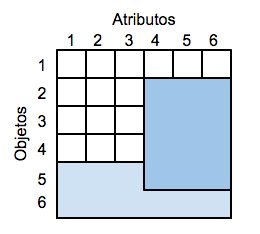
\includegraphics[width=80mm]{img/bicluster.png}
%\caption{Conjunto de dados com dois biclusters encontrados.}
%\label{fig:bicluster-exp}
%\end{figure}

% ************************************************************************

\section{Hipótese}

Fatorar matrizes considerando a decomposição da matriz original em uma matriz $U$, uma matriz $S$ e um conjunto de matrizes $V$, isto é $X \approx USV_{(1)}^T \dots V_{(k)}^T$, tal que seja possível encontrar cogrupos, possibilita que o processo de busca seja beneficiado pela flexibilidade de ajuste de $U$ e o conjunto de matrizes $V$, sendo mais adequado do que o processo tradicional de fatoração de matrizes, exposto na seção~\ref{sec:problemdef}, para o tratamento da tarefa de coagrupamento com sobreposição de colunas.
A adequação deste processo manterá informações da matriz original a fim de permitir a sua reconstrução, propiciará um resultado mais adequado em termos de agrupamento de linhas seguindo a avaliação clássica de quantização, e possibilitará a extração de informações diferenciadas a partir da análise da fatoração gerada, agregando valor à solução de um problema de mineração de texto.

% ************************************************************************

\section{Objetivos}

O objetivo geral deste trabalho foi o desenvolvimento de novas estratégias de coagrupamento baseadas em fatoração de matrizes, aqui então nomeadas \textit{OvNMTF} e \textit{BinOvNMTF}, capazes de lidar com a existência de cogrupos de colunas com sobreposição, de maneira mais adequada que os algoritmos atualmente apresentados na literatura.
A adequabilidade das estratégias propostas foi avaliada em termos de: capacidade de quantização do espaço e capacidade de reconstrução da matriz original, capacidade de agrupamento e capacidade de possibilitar a extração de informação.

Como objetivos específicos, este trabalho:

\begin{itemize}
\item apresentou a derivação formal das regras de atualização de matrizes usadas nas estratégias propostas (\textit{OvNMTF} e \textit{BinOvNMTF});
\item apresentou a aplicação das novas estratégias em ambientes controlados (bases de dados sintéticas) e em um contexto de aplicação real (análise de dado textuais);
\item apresentou um novo conjunto de dados textual, em língua portuguesa, referente ao contexto de notícias.
\end{itemize}

O atendimento aos objetivos delineados permitiu à esse trabalho:

\begin{itemize}
\item aprimorar a área de coagrupamento baseado em algoritmos de fatoração de matrizes, de forma a contribuir com a pesquisa em análise de agrupamento;
\item demonstrar que as estratégias de coagrupamento propostas têm potencial de revelar informações úteis provenientes da sobreposição natural dos atributos descritivos de um dado real, em especial para aplicações de mineração de texto.
\end{itemize}

% ************************************************************************

\section{Método}

A análise exploratória da literatura especilizada foi escolhida como estratégia para a aquisição de conhecimento sobre a área de coagrupamento e fatoração de matrizes aplicada à resolução da tarefa de coagrupamento.

A partir da análise exploratória, os algoritmos \textit{BVD}~\cite{Long2005}, \textit{ONMTF}~\cite{Ding06,Yoo2010} e \textit{FNMTF}~\cite{Wang2011} foram estudados em profundidade com o fim de verificar a sua adequabilidade para tratar a análise de coagrupamento sobre dados sintéticos e textuais, considerando a sobreposição de colunas.
Nesse estudo verificou-se a possibilidade da proposição de melhorias no tratamento do problema, e então, os algoritmos \textit{OvNMTF} e \textit{BinOvNMTF} foram criados.
Para cada um deles, o problema formal de otimização foi definido e uma derivação formal foi realizada usando cálculo em matrizes com o intuito de propor uma solução algorítmica para tais problemas.

A fim de permitir a validação das estratégias propostas e, portanto, a verificação da hipótese delineada neste trabalho, fez-se necessária a definição de: (a) um ambiente de teste controlado, representado por uma coleção de conjuntos de dados sintéticos, contendo em cada um dos conjuntos situações diferentes referentes às estruturas de coagrupamento; e (b) um contexto para realização de uma experimentação com dados reais.

Para tal experimentação foi escolhido usar o conteúdo referente à notícias publicadas no portal iG\footnote{\url{http://ig.com.br/}} e trabalhos acadêmicos publicadas na conferência \textit{NIPS}.
iG é um portal de notícias brasileiro muito conhecido, com um grande volume de notícias categorizadas em canais, os quais representam os assuntos dessas notícias.
Essas características conferem liberdade para a configuração de experimentos de diferentes naturezas, como experimentos considerando determinadas categorias de notícias, tipos de notícias ou datas de publicação das notícias.

A partir do conteúdo de notícias do portal iG foi construído um corpus de dados textuais, categorizados de acordo com as categorias já usadas no referido portal.
Todo o conteúdo do corpus passou por rotinas de pré-processamento comuns na área de mineração de texto: \textit{tokenização}~\cite{Lops2011}, filtragem de \textit{stopwords}~\cite{Lops2011}, representação da relação ``termos $\times$ documentos'' usando estratégias de frequência de termos, como $\text{\textit{tf-idf}}$~\cite{Salton1975}.

Os resultados da aplicação das estratégias de coagrupamento foram validados utilizando:

\begin{itemize}
    \item inspeção visual e erro de quantização para análise da capacidade de reconstrução;
    \item técnicas de avaliação externa representadas pelo índice de Rand e pela informação mútua normalizada, para análise da capacidade de agrupamento;
    \item análise empírica por meio de experimentos qualitativos para avaliação da capacidade de extração de informação e interpretabilidade dos modelos.
\end{itemize}

% ************************************************************************

\section{Organização do documento}

Esta dissertação é composta por $6$ capítulos incluindo esta introdução.

No capítulo~\ref{ch:conceitos} são apresentados os principais conceitos referentes à teoria de matrizes, agrupamento e coagrupamento.
O objetivo deste capítulo é fornecer diretrizes para entendimento dos assuntos tratados nos capítulos posteriores e indicar literatura na qual podem ser encontradas informações mais detalhadas sobre tais assuntos.

Estratégias de fatoração de matrizes aplicadas à resolução da tarefa de coagrupamento são discutidas no capítulo~\ref{ch:fatoracao}.
A discussão é apresentada em termos da definição de problemas e apresentação de soluções algorítmicas para os problemas.
Algumas discussões sobre os problemas e algoritmos são apresentadas sempre que um conceito é mais relevante para o entendimento da proposta deste trabalho.
Detalhes sobre cada um dos problemas e algoritmos são encontrados na literatura sugerida nesse capítulo.

A principal contribuição deste trabalho, estratégias algorítmicas baseadas em fatoração de matrizes para encontrar cogrupos com sobreposição de colunas, é apresentada em detalhes no capítulo~\ref{ch:proposedalgs}.
As definições de problemas, regras de derivação e implementações algorítimicas foram formuladas originalmente neste estudo.

Os experimentos a cerca dos algoritmos apresentados nos outros capítulos são apresentados no capítulo~\ref{ch:experiments}.
Esses experimentos ilustram a aplicabilidade e adequabilidade das estratégias apresentadas nos capítulos~\ref{ch:fatoracao} e~\ref{ch:proposedalgs}, com destaque para as vantagens e limitações das estratégias propostas neste trabalho de mestrado.
As análises apresentadas neste capítulo são de natureza quantitativa e qualitativa.

E, por fim, as conclusões deste trabalho são apresentadas no capítulo~\ref{ch:conclusoes}, destacando as contribuições aqui elaboradas e as questões em aberto na área, sendo algumas delas decorrentes de novas hipóteses, cuja formulação se tornou possível por conta das proposições realizadas no presente trabalho.

% ************************************************************
% ************************************************************
% ************************************************************

\chapter{Conceitos Fundamentais}
\label{ch:conceitos}

Este capítulo introduz os principais conceitos e definições necessárias para suportar a leitura dos demais capítulos deste trabalho.
São apresentados os conceitos e notações referentes à teoria de matrizes e álgebra linear (seção~\ref{sec:matrix-alglin}), em seguida são mostradas técnicas e conceitos referentes à agrupamento (seção~\ref{sec:clustering}), e por fim, os conceitos referentes à coagrupamento (seção~\ref{sec:coclustering}).

\section{Teoria de Matrizes e Álgebra Linear}
\label{sec:matrix-alglin}

Considere $\mathbb{R}$ o conjunto de todos os números reais, então, uma matriz no espaço $\mathbb{R}^{n \times m}$ é definida como uma tabela com $n$ linhas e $m$ colunas, na forma:
\[
    A \in \mathbb{R}^{n \times m} \Leftrightarrow A = \begin{bmatrix}
                                                                     a_{1 1} & \hdots & a_{1 m} \\
                                                                     \vdots  &        & \vdots  \\
                                                                     a_{n 1} & \hdots & a_{n m}
                                                                 \end{bmatrix}
\]
sendo $a_{i j} = (A)_{ij} \in \mathbb{R}, \forall i, j$ o elemento da $i$-ésima linha e $j$-ésima coluna da matriz $A$, e os índices $i \in \{1, \dots, n\}$ e $j \in \{1, \dots, m\}$ para indexar as linhas e colunas dessa matriz, respectivamente.
Na notação usada neste trabalho, letras maiúsculas representam matrizes (ex.: $A$), e letras minúsculas com duas letras subscritas representam valores na matriz (ex.: $a_{ij}$ representa um valor da matriz $A$).
Também é possível definir essa mesma matriz em $\mathbb{R}^{n \times m}_{+}$, por meio da determinação da restrição $a_{ij} > 0, \forall i,j$.

De forma semelhante define-se uma notação para vetores no espaço $\mathbb{R}^n$, na forma:
\[
    \mathbf{a} \in \mathbb{R}^n \Leftrightarrow \mathbf{a} = \begin{bmatrix}
                                                                     a_{1}  \\
                                                                     \vdots \\
                                                                     a_{n}
                                                                 \end{bmatrix}
\]
sendo $a_i \in \mathbb{R}, \forall i$ o $i$-ésimo elemento do vetor.
Ainda, neste trabalho, é usada a notação de vetores para representação das linhas e colunas de uma matriz, da seguinte forma:
\[
    A = \begin{bmatrix}
            \horzbar & \mathbf{a}_{1 \cdot} & \horzbar \\
                     & \vdots               &          \\
            \horzbar & \mathbf{a}_{n \cdot} & \horzbar
        \end{bmatrix}
      = \begin{bmatrix}
            \vertbar             &          & \vertbar             \\
            \mathbf{a}_{\cdot 1} & \dots    & \mathbf{a}_{\cdot m} \\
            \vertbar             &          & \vertbar
        \end{bmatrix}
\]
sendo $\mathbf{a}_{i \cdot}$ e $\mathbf{a}_{\cdot j}, \forall i,j$ os vetores que representam as linhas e colunas da matriz $A$, respectivamente.

Neste trabalho as seguintes operações em matrizes são usadas~\cite{Golub1996}:
\begin{itemize}
    \item Transposição de matrizes: $(A^T)_{ij} = (A)_{ji}, \forall i, j$, $A^T \in \mathbb{R}^{m \times n}$, $A \in \mathbb{R}^{n \times m}$.
    \item Produto de Hadamard: $C=A\odot B$, onde $c_{ij} = a_{ij} b_{ij}, \forall i, j$, sendo $A, B, C \in \mathbb{R}^{n \times m}$.
    \item Divisão de matrizes ponto-a-ponto: $C = \frac{A}{B}$, onde $c_{ij} = \frac{a_{ij}}{b_{ij}}$, $\forall i, j$, sendo $A, B, C \in \mathbb{R}^{n \times m}$.
    \item Produto de matrizes: $C = AB$, onde $c_{ij} = \sum_{p = 1}^k$ $a_{ip} b_{pj}$, sendo $C \in \mathbb{R}^{n \times m}, A \in \mathbb{R}^{n \times k}, B \in \mathbb{R}^{k \times m}$.
    \item Matriz inversa: $AB = BA = I \Leftrightarrow B = A^{-1}$, sendo $A \in \mathbb{R}^{n \times n}, B \in \mathbb{R}^{n \times n}$, e $I$ a matriz identidade.
\end{itemize}

Para definição de problemas em fatoração, também é usado neste trabalho um operador: traço da matriz.
Considerando uma matriz quadrada $A \in \mathbb{R}^{n \times n}$~\cite{Magnus1999}, o traço da matriz é definido da seguinte forma:
\[
    tr(A) = \sum_{i=1}^n a_{ii}
\]
Algumas igualdades são possíveis a partir da aplicação deste operador.
Considerando as matrizes $A, B, C$, em um espaço que torne as multiplicações possíveis, definem-se as seguintes igualdades~\cite{Magnus1999}:
\begin{itemize}
    \item $tr(A^T) = tr(A)$.
    \item $tr(A^TB) = tr(B^TA)$.
    \item $tr(AB) = tr(BA)$.
    \item $tr(ABC) = tr(CAB) = tr(BCA)$ (propriedade circular).
\end{itemize}
Note que a matriz resultante das operações dentro do traço é sempre quadrada.

Definido o operador de traço, é possível definir o operador para o produto interno entre dois vetores $\mathbf{a}, \mathbf{b} \in \mathbb{R}^n$~\cite{Boyd2004}, da seguinte forma:
\[
    \langle \mathbf{a}, \mathbf{b} \rangle = \sum_{i=1}^n a_i b_i = \begin{bmatrix}
                                                                        a_{1} & \dots & a_{n}
                                                                    \end{bmatrix}
                                                                    \begin{bmatrix}
                                                                        b_{1}  \\
                                                                        \vdots \\
                                                                        b_{n}
                                                                    \end{bmatrix}
                                                                  = \mathbf{a}^T \mathbf{b}
\]

Da mesma forma define-se o produto interno entre duas matrizes $A \in \mathbb{R}^{n \times m}$ e $B \in \mathbb{R}^{n \times m}$, mostrando como os operadores de traço e produto interno se relacionam~\cite{Boyd2004}:
\[
    \langle \mathbf{A}, \mathbf{B} \rangle = \sum_{i=1}^n \sum_{j=1}^m a_{ij} b_{ij} = tr(A^TB)
        % \begin{bmatrix}
        %     \vertbar             &          & \vertbar             \\
        %     \mathbf{a}_{\cdot 1} & \dots    & \mathbf{a}_{\cdot n} \\
        %     \vertbar             &          & \vertbar
        % \end{bmatrix}
        % \begin{bmatrix}
        %     \horzbar & \mathbf{b}_{1 \cdot} & \horzbar \\
        %              & \vdots               &          \\
        %     \horzbar & \mathbf{b}_{n \cdot} & \horzbar
        % \end{bmatrix}
        % = tr(A^TB)
\]

\subsection{Norma em matrizes}

A norma é uma função que recebe como parâmetro de entrada um vetor ou uma matriz nos espaços $\mathbb{R}^n$ ou $\mathbb{R}^{n \times m}$, respectivamente, e gera um valor real, o qual representa a magnitude do vetor ou matriz.
Uma das normas mais conhecidas é a norma de Frobenius, usada nas definições dos problemas de fatoração deste trabalho.
A norma de Frobenius é definida da seguinte forma para um vetor $\mathbf{a} \in \mathbb{R}^n$~\cite{Boyd2004}:
\[
    \norm{\mathbf{a}}_F = \sqrt{a_1^2 + \dots + a_n^2} = \sqrt{\mathbf{a}^T \mathbf{a}} = \sqrt{\langle \mathbf{a}, \mathbf{a} \rangle}
\]
Essa norma também é chamada de norma Euclidiana e $\text{norma-}L_2$.
Neste caso, a norma é definida da seguinte forma para uma matriz $A \in \mathbb{R}^{n \times m}$~\cite{Boyd2004}:
\[
    \norm{A}_F = \sqrt{\sum_{i=1}^n \sum_{j=1}^m |a_{ij}^2|} = \sqrt{tr(A^T A)}
\]

Ainda, considerando dois vetores $\mathbf{a}$ e $\mathbf{b}$, é possível dizer que estes são ortogonais se o produto interno entre eles for $0$, ou seja, não há projeção de $\mathbf{a}$ em $\mathbf{b}$, e vice-versa~\cite{Magnus1999}:
\[
    \langle \mathbf{a}, \mathbf{b} \rangle = 0
\]
Os vetores $\mathbf{a}$ e $\mathbf{b}$ também podem ser ditos ortonormais se, além da condição anterior, as suas normas forem igual à $1$.
A mesma definição pode ser estendida para matrizes, então, uma matriz é dita ortonormal se todos os seus vetores forem ortonormais~\cite{Magnus1999}:
\[
    A^T A = I
\]

\subsection{Cálculo em matrizes}
\label{subsec:matrixcalculus}

Cálculo em matrizes define uma notação que suportou a derivação de soluções para os problemas de otimização, baseados em fatoração de matrizes, propostos neste trabalho.
Estendendo a definição de derivadas, tradicionalmente conhecida, é possível obter relações para derivação de funções em relação a matrizes~\cite{Magnus1999}.
Considere a seguinte notação para derivada de uma função de traço em relação à uma matriz $A$, sendo $F(A)$ uma função diferenciável em todos os elementos de $A$~\cite{Petersen2012}:
\[
    \frac{\partial tr(F(A))}{\partial A} = f(A)^T
\]
em que $f(\cdot)$ é a derivada escalar de $F(\cdot)$.

Diante desta definição, algumas relações podem ser mostradas~\cite{Petersen2012}.
Sendo $A, B, C$ e $D$ matrizes quaisquers definidas em um espaço que tornem as multiplicações possíveis, para cada caso:
\begin{itemize}
    \item $\frac{\partial}{\partial A} tr(A) = I$ (matriz identidade).
    \item $\frac{\partial}{\partial A} tr(B A) = B^T$.
    \item $\frac{\partial}{\partial A} tr(B A^T) = \frac{\partial}{\partial A} tr(A^T B) = B$.
    \item $\frac{\partial}{\partial A} tr(B A C) = B^T C^T$.
    \item $\frac{\partial}{\partial A} tr(B A^T C) = CB$.
    \item $\frac{\partial}{\partial A} tr(B A C A^T D) = B^T D^T A C^T + D B A C$.
    \item $\frac{\partial}{\partial A} tr(C^T A^T D A C) = C^T A^T D B + C^T A^T B^T D^T$.
\end{itemize}

\section{Agrupamento}
\label{sec:clustering}

Classicamente, a tarefa de agrupamento de dados é definida como o processo de agrupar dados de acordo com a similaridade existente entre eles.
Sendo assim, os dados alocados a um mesmo grupo são aqueles mais similares entre si, enquanto que os dados alocados em grupos diferentes são dissimilares entre si.
Nesse contexto, similaridades, e dissimilaridades, são geralmente calculadas por meio de medidas de distâncias~\cite{Han2011}.
A tarefa de agrupamento pode também ser vista como um processo de particionamento das linhas de uma matriz que representa um conjunto de dados, sendo que esse conjunto de dados contém dados e características desses dados~\cite{Han2011}.
Ainda, os grupos podem ser vistos como uma forma de compressão de dados.

A tarefa de agrupamento pode ser resolvida a partir de técnicas provenientes da área de aprendizado de máquina, mais especificamente por um subconjunto de técnicas de aprendizado não-supervisionado, nas quais tem-se mecanismos para realizar análise de dados para os quais não se tem informação a priori sobre como os dados estão organizados.
A resolução da tarefa de agrupamento pode ser útil em diversas áreas do conhecimento, tais como Mineração de Dados, Estatística, Tomada de Decisão, etc.

Formalmente, os algoritmos de agrupamento implementados sob estratégias de particionamento têm como entrada uma matriz de dados $X \in \mathbb{R}^{n \times m}$, com $n$ linhas (dados) e $m$ colunas (características) que representam um conjunto de dados em algum domínio de aplicação.
Essa matriz é formada por um conjunto de vetores de linhas $\mathcal{N} = \{ \mathbf{x}_{1 \cdot}, \dots, \mathbf{x}_{n \cdot} \}$.
O objetivo é encontrar $k$ partições de $\mathcal{N}$, denotadas por subconjuntos ordenados $\mathcal{K}_p \subseteq \mathcal{N}$, considerando o índice $p \in \{ 1, \dots, k\}$.
Então, o conjunto $\mathscr{K} = \{\mathcal{K}_1, \dots, \mathcal{K}_k\}$ é justamente os grupos de linhas resultantes de um algoritmo que soluciona a tarefa de agrupamento.
Note que este problema é NP-difícil, então faz sentido buscar por algoritmos que se baseiam em alguma heurística, já que não existe uma solução algorítmica em tempo polinomial~\cite{Aloise2009}.

\subsection{Algoritmos para Agrupamento}
\label{sec:clustering:algos}

O problema de agrupamento \textit{k-means} é provavelmente um dos problemas mais estudados para agrupamento, e o algoritmo de \textit{Lloyd}, também chamado algoritmo \textit{k-means}, é um dos algoritmos mais famosos para solução do problema de agrupamento.
Trata-se de um problema de otimização do erro de quantização, formalizado no problema~\ref{def:kmeans:problem}, proposto com o objetivo de encontrar grupos em um conjunto de dados, solucionando a tarefa de agrupamento.

O objetivo do \textit{k-means} é encontrar $k$ representantes da matriz de dados $X$.
Esses representantes, também chamados centróides ou médias, são organizados em uma matriz $C$ com $k$ linhas e $m$ colunas, sendo que cada vetor de linha é um representante dos dados, por isso estes têm a mesma dimensão dos dados da matriz $X$.
De forma direta é possível perceber que serão formados $k$ grupos de dados.

Neste trabalho o problema \textit{k-means} é mostrado sob uma visão de fatoração de matrizes, assim como em~\citeonline{Ding05}, pois tem-se como objetivo encontrar uma solução para aproximar $X$ pela multiplicação de duas matrizes $U$ e $C$: $X \approx UC$.
Além disso, em~\citeonline{Ding05} também é mostrada a relação de aproximação entre os algoritmos de agrupamento mais tradicionais, como o \textit{k-means}, o \textit{fuzzy k-means} e o problema de Fatoração de Matrizes Não-negativas (NMF - \textit{Non-negative Matrix Factorization}), que apesar de ter sido desenvolvido como um método de redução de dimensionalidade, também é considerado um método de agrupamento.

\begin{problem}[Problema de \textit{k-means}]
\label{def:kmeans:problem}
\begin{equation}
    \begin{array}{lclcl}
        \displaystyle \mathcal{F}_1(U, C) & = & \displaystyle \min_{U, C} \sum_{i=1}^n \sum_{p=1}^k u_{ip} \norm{\mathbf{x_{i \cdot} - \mathbf{c_{p \cdot}}}}^2 = \displaystyle \min_{U, C} & \norm{X - UC}^{2}_{F} \\
                                          &   & \text{suj. a}                & U \in \Psi^{n \times k}, \\
                                          &   &                              & C \in \mathbb{R}^{k \times m}, \\
                                          &   &                              & \sum_{p=1}^{k} u_{ip} = 1, \forall i
    \end{array} \nonumber
\end{equation}
em que $\Psi = \{0, 1\}$ e $\norm{\cdot}_F$ denota a norma de Frobenius para matrizes.
\end{problem}

A restrição da soma de cada linha da matriz $U$ ser igual à $1$, garante que cada dado de $X$ pertença a apenas um grupo, já que o objetivo é particionar os dados.

É possível perceber que o problema apresentado compacta a matriz $X$ em duas outras matrizes: a matriz $U$, de dimensão $n$ por $k$ que contém apenas valores binários, e fará a associação de cada linha de $X$ com um dos $k$ grupos; e a matriz $C$, de dimensão $k$ por $m$, que será uma base para representação das linhas em $X$.
Portanto, a compactação transformará os $nm$ elementos originais em $n + km$ novos elementos, desconsiderando os zeros da matriz $U$.

A implementação para o problema~\ref{def:kmeans:problem} é descrito no algoritmo~\ref{algo:kmeans}~\cite{Peres2012,Han2011,Bottou95}, o qual é baseado no algoritmo de EM (Esperança-Maximização - \textit{Expectation-Maximization}) e tem sua convergência para um mínimo local demonstrada (veja em~\citeonline{Bottou95}).
Nesse algoritmo considere os índices $i \in \{1, \dots, n\}$ e $p, p' \in \{1, \dots, k\}$, $t$ o contador de iterações, $U^{(t)}$ e $C^{(t)}$ as matrizes $U$ e $C$ na iteração $t$, respectivamente, $\mathcal{U}(0, 1) \in~]0, 1]$ uma função que gera valores de uma distribuição uniforme, e $\norm{ \cdot }^2$ é a norma de Frobenius para vetores.

\begin{algorithm}
\caption{Algoritmo para solução do \textit{k-means}}
\label{algo:kmeans}
    \begin{algorithmic}[1]
        \Function{k-means}{$X$, $k$, $t_{max}$}
            \State \textbf{Inicialize:} $C^{(0)} \gets \mathcal{U}(0, 1)$ e $t \gets 0$.
            \While{(não convergiu) e ($t \leq t_{max}$)}
                \State
                    \begin{equation}
                    \label{eq:kmeans:updateU}
                        (U^{(t+1)})_{ip} \gets \left\{
                            \begin{array}{ll}
                                1 & p = \argmin_{p' \in \{1, \dots, k\}} \norm{ \mathbf{x}_{i \cdot} - \mathbf{c}^{(t)}_{p' \cdot} }^2 \\
                                0 & \textit{caso contrário}
                            \end{array}    \nonumber
                        \right. \forall i, p
                    \end{equation}
                    \Comment{Etapa de Esperança}
                \State
                    \begin{equation}
                    \label{eq:kmeans:updateC}
                        (C^{(t+1)})_{p \cdot} \gets \frac{\sum_{i=1}^{n} u_{ip}^{(t+1)} \mathbf{x}_{i \cdot} }{\sum_{i=1}^{n} u_{ip}^{(t+1)}}, \forall p \nonumber
                    \end{equation}
                    \Comment{Etapa de Maximização}
                \State $t \gets t + 1$
            \EndWhile\label{euclidendwhile}
            \State \textbf{return} $U^{(t)}, C^{(t)}$
        \EndFunction
    \end{algorithmic}
\end{algorithm}

Como condições para assumir a convergência, neste trabalho, considera-se a diferença do erro de aproximação em duas iterações consecutivas menor ou igual a um $\epsilon$:
$$\norm{X - U^{(t)} C^{(t)}}^{2}_{F} - \norm{X - U^{(t+1)} C^{(t+1)}}^{2}_{F} \leq \epsilon$$
O algoritmo também pára caso a $t$-ésima iteração seja igual ao número máximo de iterações ($t_{max}$).
Note que o particionamento é direto, analisando a matriz $U$.

Ainda, a atualização de $C$ também pode ser derivada de forma matricial, expandindo a função apresentada no problema~\ref{def:kmeans:problem} e derivando em relação à $C$, usando as relações definidas na seção~\ref{subsec:matrixcalculus}.
Assim, obtém-se a seguinte formulação, que é equivalente à apresentada no algoritmo~\ref{algo:kmeans}~\cite{Bauckhage2015}:
\[
    C = (U^T U)^{-1} U^T X
\]

O algoritmo \textit{k-means} tem complexidade de tempo $\mathcal{O}(t_{max} nmk)$.
Isso mostra a escalabilidade do algoritmo para grandes bases de dados, ou seja, matrizes com $n$ e/ou $m$ grandes~\cite{Han2011}.

Outro problema semelhante ao \textit{k-means} é o \textit{fuzzy k-means}, o qual, ao invés de restringir a pertinência de cada dado a exclusivamente um grupo, permite que o dado pertença a diferentes grupos com diferentes graus de pertinência.
Então, a matriz $U$ será a matriz responsável por armazenar a pertinência de cada dado (ou linha) de $X$ a cada um dos $k$ grupos.

O problema de otimização do erro de quantização, com a finalidade da resolução da tarefa de agrupamento (\textit{fuzzy k-means}), é apresentado formalmente no problema~\ref{def:fkmeans:problem}~\cite{Bezdek1981,Peres2012,Ding05}.

\begin{problem}[Problema de \textit{fuzzy k-means}]
\label{def:fkmeans:problem}
\begin{equation}
    \begin{array}{lclcl}
        \displaystyle \mathcal{F}_2(U, C) & = & \displaystyle \min_{U, C}    & \sum_{i=1}^n \sum_{p=1}^k u_{ip}^w \norm{\mathbf{x_{i \cdot} - \mathbf{c_{p \cdot}}}}^2 \\
                                          &   & \text{suj. a}                & U \in \mathbb{R}^{n \times k}, \\
                                          &   &                              & C \in \mathbb{R}^{k \times m}, \\
                                          &   &                              & \sum_{p=1}^{k} u_{ip} = 1, \forall i
    \end{array} \nonumber
\end{equation}
em que $w \in [1, 2, \dots, \infty]$.
\end{problem}

O expoente $w$ é chamado de parâmetro de ``fuzificação'', e tem a função de controlar a relação de pertinência de um dado entre os $k$ grupos, isto é, pode se dizer que o parâmetro controla a ortogonalidade dos grupos, quanto maior o seu valor, menor a ortogonalidade entre grupos.
Isso pode ser percebido, observando a análise de limite de $w$ na função de atualização de $U$, realizada em~\citeonline{Peres2012}.

Se $w = 2$ é possível modificar o problema~\ref{def:fkmeans:problem} tal que seja possível observá-lo sob uma ótica de fatoração de matrizes, que tem o objetivo de aproximar $X$ das matrizes $U$ e $C$, assim como no \textit{k-means}: $X \approx UC$.
O problema~\ref{def:fkmeans:problem} é apresentado com $w = 2$ para obtenção da ótica de fatoração de matrizes~\cite{Ding05}:
\[
\begin{array}{lclcl}
    \displaystyle \mathcal{F}_{2}^{w=2}(U, C) & = & \displaystyle \min_{U, C} \sum_{i=1}^n \sum_{p=1}^k u_{ip}^2 \norm{\mathbf{x_{i \cdot} - \mathbf{c_{p \cdot}}}}^2 = \min_{U, C} & \norm{X - UC}^{2}_{F} \\
                                              &   & \text{suj. a}                & U \in \mathbb{R}^{n \times k}, \\
                                              &   &                              & C \in \mathbb{R}^{k \times m}, \\
                                              &   &                              & \sum_{p=1}^{k} u_{ip} = 1, \forall i
\end{array}
\]

Da mesma forma que o \textit{k-means}, o \textit{fuzzy k-means} compacta os dados de $X$, sendo um mapeamento de $nm$ elementos para $nk + km$ elementos.
Então, teoricamente, o \textit{fuzzy k-means} é capaz de preservar mais informações do que o \textit{k-means}.

A implementação para o problema~\ref{def:fkmeans:problem} é descrita no algoritmo~\ref{algo:fkmeans}~\cite{Peres2012,Ding05,Bezdek1981}, o qual é baseado na combinação do algoritmo \textit{k-means} com conceitos da teoria de conjuntos fuzzy e tem sua convergência para um mínimo local demonstrada via teoria de otimização não-linear (veja em~\citeonline{Bezdek1981}).
Nesse algoritmo considere os índices $i \in \{1, \dots, n\}$ e $p, p' \in \{1, \dots, k\}$, $t$ o contador de iterações, $U^{(t)}$ e $C^{(t)}$ as matrizes $U$ e $C$ na iteração $t$, respectivamente, $\mathcal{U}(0, 1) \in~]0, 1]$ uma função que gera valores de uma distribuição uniforme, e $\norm{ \cdot }^2$ é a norma de Frobenius para vetores.
Ainda, a mesma condição de convergência aplicada ao algoritmo~\ref{algo:kmeans} pode ser aplicada para esse algoritmo.

\begin{algorithm}
\caption{Algoritmo para solução do \textit{fuzzy k-means}}
\label{algo:fkmeans}
    \begin{algorithmic}[1]
        \Function{fuzzy k-means}{$X$, $k$, $t_{max}$}
            \State \textbf{Inicialize:} $C^{(0)} \gets \mathcal{U}(0, 1)$ e $t \gets 0$.
            \While{(não convergiu) e ($t \leq t_{max}$)}
                \State
                    \begin{equation}
                    \label{eq:fkmeans:updateU}
                        (U^{(t+1)})_{ip} \gets \Bigg[ \sum_{p'=1}^k \Bigg( \frac{\norm{\mathbf{x}_{i \cdot} - \mathbf{c}^{(t)}_{p \cdot}}}{\norm{\mathbf{x}_{i \cdot} - \mathbf{c}^{(t)}_{p' \cdot}}} \Bigg)^{\frac{1}{w - 1}} \Bigg]^{-1}, \forall i,p \nonumber
                    \end{equation}
                \State
                    \begin{equation}
                    \label{eq:fkmeans:updateC}
                        (C^{(t+1)})_{p \cdot} \gets \frac{\sum_{i=1}^{n} u_{ip}^{w^{(t+1)}} \mathbf{x}_{i \cdot} }{\sum_{i=1}^{n} u_{ip}^{w^{(t+1)}}}, \forall p \nonumber
                    \end{equation}

                \State $t \gets t + 1$
            \EndWhile\label{euclidendwhile}
            \State \textbf{return} $U^{(t)}, C^{(t)}$
        \EndFunction
    \end{algorithmic}
\end{algorithm}

Note que como $U$ possui valores no domínio dos reais, não é possível obter as partições diretamente, sem um processo de pós-processamento.
Um método de pós-processamento é o seguinte:
$$\mathcal{K}_{p} = \{ x_{i\cdot}~|~i \in \{1,\dots,n\} \text{ e } p = \argmax_{p'\in\{1, \dots, k\}} u_{ip'} \}, \forall p \in \{1, \dots, k\}$$
Isso significa que uma linha $i$ pertencerá a um grupo $p$ (ou partição) se para todos os $k$ grupos, o grau de pertinência $u_{ip}$ for maior que todos os outros graus de pertinência para os outros grupos, presentes no vetor $\mathbf{u}_{i \cdot}$. Analisando a complexidade de tempo do algoritmo é possível chegar em: $\mathcal{O}( t_{max} nmk^2 )$.

Além dos algoritmos apresentados, existem outros que buscam resolver diferentes tipos de problemas dentro da área de agrupamento, como agrupamento por densidade, agrupamento hierárquico, agrupamento baseado em grade e agrupamento baseado em modelos~\cite{Han2011}.

\subsection{Validação de Agrupamento}
\label{sec:clustering:eval}

Para avaliar a qualidade de um agrupamento obtido a partir da execução de um algoritmo, e consequentemente, avaliar a adequabilidade dos parâmetros usados nesse algoritmo, a capacidade de agrupamento ou a estabilidade do processo por ele executado, é necessário fazer uso de métricas de validação (ou avaliação).
Como neste trabalho são feitas comparações entre diversos algoritmos quanto às suas capacidades de agrupamento, os métodos e métricas estudados na área de validação de agrupamento precisam ser estudados, pois trazem recursos e ferramentas que tornam possíveis análises quantitativas, considerando os resultados de agrupamento desses algoritmos.

\citeonline{Halkidi2002a, Halkidi2002b} propõem a seguinte taxonomia para métricas de validação de agrupamento: \textit{validação interna}, que utiliza apenas o resultado de um agrupamento gerado para estabelecer métricas de qualidade ou estabilidade, permitindo avaliar as soluções geradas; \textit{validação externa}, tem como entrada para o cálculo das medidas dois tipos de informação: o particionamento real dos dados, e o resultado de um agrupamento gerado - essas informações são usadas para verificar o quanto o agrupamento gerado corresponde ao particionamento real; e \textit{validação relativa}, que analisa diferentes soluções geradas por um mesmo algoritmo diante de diferentes parametrizações, e estabelece métricas para encontrar a melhor solução dentre as soluções disponíveis.

Neste trabalho, são utilizadas apenas métricas de validação externa para validar a capacidade de agrupamento dos diferentes algoritmos apresentados.
Dentre as muitas métricas de validação externa presentes na literatura~\cite{Halkidi2002a,Halkidi2002b}, foram escolhidas as métricas Índice de Rand ($\text{\textit{RI}}$ - \textit{Rand Index})~\cite{Rand1971} e Informação Mútua Normalizada ($\text{\textit{NMI}}$ - \textit{Normalized Mutual Information}).

O RI gera valores entre $0$ e $1$, com $0$ indicando que o particionamento de dados gerado por um algoritmo não concorda em nenhum par de elementos com o particionamento real, e $1$ indicando que o particionamento gerado pelo mesmo algoritmo é exatamente igual ao particionamento real.

Considere que um algoritmo encontrou um particionamento denotado pelo conjunto $\mathscr{\widetilde{K}} = \{\mathcal{\widetilde{K}}_1, \dots, \mathcal{\widetilde{K}}_{\widetilde{k}}\}$ com $\widetilde{k}$ grupos, sendo $\mathcal{\widetilde{K}}_p, \forall p \in \{1, \dots, \widetilde{k}\}$ um subconjuto que contém elementos pertencentes ao $p$-ésimo grupo.
Considere também, o particionamento real: $\mathscr{K} = \{\mathcal{K}_1, \dots, \mathcal{K}_k\}$ com $k$ grupos.
Então, determine as seguintes quantidades, sendo os dados as linhas da matriz de dados $X$ denotado pelo conjunto $\mathcal{N}$:
\begin{itemize}
    % \item a: quantidade de pares de elementos (elementos distintos) para os quais os elementos pertencem a uma mesma partição no particionamento gerado e a uma mesma partição no particionamento real;
    % \item b: quantidade de pares de elementos (elementos distintos) para os quais os elementos pertencem a uma mesma partição no particionamento gerado e a partições diferentes no particionamento real;
    % \item c: quantidade de pares de elementos (elementos distintos) para os quais os elementos pertencem à partições diferentes no particionamento gerado e a uma mesma partição no particionamento real;
    % \item d: quantidade de pares de elementos para os quais os elementos pertencem à partições diferentes no particionamento gerado e a partições diferentes no particionamento real.
    \item $a$: quantidade de pares de dados em $\mathcal{N}$ que estão nos mesmos subconjuntos em $\mathscr{K}$ e também nos mesmos subconjuntos em $\mathscr{\widetilde{K}}$;
    \item $b$: quantidade de pares de dados em $\mathcal{N}$ que estão em diferentes subconjuntos em $\mathscr{K}$ e também estão em diferentes subconjuntos em $\mathscr{\widetilde{K}}$;
    \item $c$: quantidade de pares de dados em $\mathcal{N}$ que estão nos mesmos subconjuntos em $\mathscr{K}$ e em diferentes subconjuntos em $\mathscr{\widetilde{K}}$;
    \item $d$: quantidade de pares de dados em $\mathcal{N}$ que estão em diferentes subconjuntos em $\mathscr{K}$ e estão nos mesmos subconjuntos em $\mathscr{\widetilde{K}}$.
\end{itemize}

Note então, que $a$ e $b$ denotam que o resultado de particionamento do algoritmo está de acordo com o particionamento real, e $c$ e $d$ denotam que o particionamento resultante do algoritmo não está de acordo com o particionamento real.

Sendo assim, o Índice de Rand ($\text{\textit{RI}}$) pode ser definido pela fração com que o particionamento obtido está de acordo com o particionamento real, da seguinte forma:
\[
    \text{\textit{RI}}(\mathscr{K}, \mathscr{\widetilde{K}}) = \frac{a + b}{a + b + c + d}
\]

A métrica de validação externa, $\text{\textit{NMI}}$, tem efeito semelhante ao RI~\cite{Manning2008}.
Utilizando a mesma notação, essa métrica é baseada na Informação Mútua (MI - \textit{Mutual Information}) entre o resultado de particionamento de um algoritmo ($\mathscr{\widetilde{K}}$) e o particionamento real ($\mathscr{K}$), e gera valores entre $0$ e $1$, com $0$ indicando que não há informação mútua entre $\mathscr{K}$ e $\mathscr{\widetilde{K}}$, e $1$ indicando correlação perfeita entre $\mathscr{K}$ e $\mathscr{\widetilde{K}}$.
Então $\text{\textit{MI}}$ é definido da seguinte forma:
\[
    \text{\textit{MI}}(\mathscr{K}, \mathscr{\widetilde{K}}) = \displaystyle \sum_{p=1}^k \sum_{p'=1}^{\widetilde{k}} \frac{|\mathcal{K}_p \cap \mathcal{\widetilde{K}}_{p'}|}{n} \log \frac{n |\mathcal{K}_p \cap \mathcal{\widetilde{K}}_{p'}|}{|\mathcal{K}_p| |\mathcal{\widetilde{K}}_{p'}|}
\]
A normalização de $\text{\textit{MI}}$ é realizada usando a entropia dos particionamentos.
A entropia de um particionamento, $H(\cdot)$, é dada da seguinte forma:
\[
    H(\mathscr{K}) = \displaystyle \sum_{p=1}^k \frac{\mathcal{K}_p}{n} \log \frac{\mathcal{K}_p}{n}
\]
Finalmente, a métrica $\text{\textit{NMI}}$ pode ser definida como:
\[
    \text{\textit{NMI}}(\mathscr{K}, \mathscr{\widetilde{K}}) = \frac{\text{\textit{MI}}(\mathscr{K}, \mathscr{\widetilde{K}})}{\sqrt{H(\mathscr{K}) H(\mathscr{\widetilde{K}})}}
\]

Note, então, que ambas as métricas têm capacidade de lidar com a caso em que a ordem do particionamento no conjunto $\mathscr{K}$ não corresponde com a ordem do particionamento no conjunto $\mathscr{\widetilde{K}}$.
Além disso, ambas as métricas têm sido efetivas como um método de análise quantitativa na análise de qualidade de agrupamento entre diferentes algoritmos, principalmente no que diz respeito ao domínio de agrupamento de documentos~\cite{Kuang2014,Ho2008,Wang2011,Ding06,Xu2003,Yoo2010}.

\section{Coagrupamento}
\label{sec:coclustering}

Grande parte dos esforços de pesquisa da área de mineração de dados é voltada ao estudo da tarefa de agrupamento~\cite{Han2011}, no entanto, ainda há muito estudo a ser realizado quando se considera dados com alta dimensionalidade e/ou quando se deseja interpretabilidade do agrupamento gerado por um algoritmo.

Nesse contexto, faz-se interessante analisar de forma mais detalhada, as características que, dentre todas as disponíveis, tornam os dados mais similares entre si a ponto de poderem ser associados a um mesmo grupo.
Mais do que isso, a ideia é saber se ao considerar apenas parte das características, um dado pode ser associado a um grupo diferente.
Essa análise leva ao estudo de questões referentes a estratégias capazes de usar a similaridade baseada em partes, a qual analisa subconjuntos de características.
Um dos primeiros trabalhos a tratar esse tipo de problema foi apresentado por~\citeonline{Hartigan1972}.
Nesse trabalho, o autor apresenta métodos de agrupamento de dados que particionam tanto os dados quanto as características, a análise das partições, e uma taxonomia referente às diversas estruturas que essas partições podem compor.

Com o passar do tempo, esse problema foi se tornando mais presente em aplicações reais, nas mais diferentes áreas, como Mineração de Textos, Mineração da Web, Bioinformática, Marketing, Ecologia, Arqueologia e Ciência da Computação~\cite{Govaert2013}.
E hoje, o processo de agrupamento que se baseia na similaridade em partes das características é conhecido como coagrupamento ou biagrupamento.
O termo biagrupamento é usado principalmente no contexto de expressão genética, enquanto o termo coagrupamento é usado principalmente em aplicações de mineração de texto.

Os algoritmos do processo de coagrupamento são capazes de gerar grupos de dados levando em consideração todas as características, ou apenas algumas características~\cite{Franca2010,Madeira2004}.
Existem diversas maneiras de visualizar o problema de coagrupamento, uma visão importante é de encontrar submatrizes de uma matriz de dados, formalizando~\cite{Madeira2004}: tem-se uma matriz $X$, de dimensão $n \times m$, formada por um conjunto de vetores de linhas $\mathcal{N} = \{ \mathbf{x}_{1 \cdot}, \dots, \mathbf{x}_{n \cdot} \}$ e um conjunto de vetores de colunas $\mathcal{M} = \{ \mathbf{x}_{\cdot 1}, \dots, \mathbf{x}_{\cdot m} \}$.
O problema de coagrupamento, dentro desta visão, é encontrar cogrupos, que são submatrizes de $X$, denotados por $X_{\mathcal{K}_p \mathcal{L}_q}$, considerando $k$ subconjuntos ordenados $\mathcal{K}_p \subseteq \mathcal{N}$, $l$ subconjuntos ordenados $\mathcal{L}_q \subseteq \mathcal{M}$, e os índices $p \in \{ 1, \dots, k\}$ e $q \in \{1, \dots, l\}$.
Assim, o cogrupo $X_{\mathcal{K}_p \mathcal{L}_q}$ é um grupo dos dados em $\mathcal{K}_p$, perante as características em $\mathcal{L}_q$.

Essa visão do problema de coagrupamento está ilustrada na figura~\ref{fig:bicluster-exp}, na qual é apresentado um conjunto de dados que possui as linhas (dados) $\mathbf{x}_{1 \cdot}, \mathbf{x}_{2 \cdot}, \mathbf{x}_{2 \cdot}, \mathbf{x}_{4 \cdot}, \mathbf{x}_{5 \cdot}$ e $\mathbf{x}_{6 \cdot}$ que são representados pelas colunas (características) $\mathbf{x}_{1 \cdot}, \mathbf{x}_{\cdot 2}, \mathbf{x}_{\cdot 3}, \mathbf{x}_{\cdot 4}, \mathbf{x}_{\cdot 5}$ e $\mathbf{x}_{\cdot 6}$, sendo $n,m = 6$.
Na figura~\ref{fig:bicluster-exp} também estão ilustrados dois cogrupos hipotéticos: o primeiro formado pelas linhas $\mathbf{x}_{5 \cdot}$ e $\mathbf{x}_{6 \cdot}$ e todos os atributos $\mathbf{x}_{\cdot 1}, \dots, \mathbf{x}_{\cdot 6}$, representando um cogrupo com \textit{modelo global}; e o segundo formado pelos objetos $\mathbf{x}_{2 \cdot}, \mathbf{x}_{3 \cdot}, \mathbf{x}_{4 \cdot}$ e $\mathbf{x}_{5 \cdot}$, e as características $\mathbf{x}_{\cdot 4}, \mathbf{x}_{\cdot 5}$ e $\mathbf{x}_{\cdot 6}$, representando um cogrupo com \textit{modelo local}, que leva em consideração apenas um subconjunto dos atributos.

\begin{figure}[H]
\centering
    \caption{Conjunto de dados com dois cogrupos}
    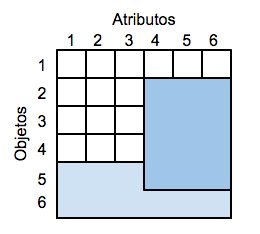
\includegraphics[width=0.55\textwidth]{img/bicluster.png}
    \label{fig:bicluster-exp}
\source{Adaptado de \citeonline{Madeira2004}}
\end{figure}

Como a definição apresentada não inclui uma estrutura a priori da matriz $X$ e dos cogrupos $X_{\mathcal{K}_p \mathcal{L}_q}$, os algoritmos propostos na literatura diferem quanto ao tipo de cogrupo que são capazes de encontrar.
Uma taxonomia dos tipos de cogrupos é proposta por~\citeonline{Madeira2004}:
 \begin{itemize}
 %  \item \textit{Cogrupos com valores constantes}, se trata de cogrupos em que todos os valores de são constantes: $\mu_{pq} \in X_{\mathcal{K}_p \mathcal{L}_q}, \forall p, q$, onde $\mu_{pq}$ é um valor constante para um cogrupo. Porém, em conjuntos de dados reais, esses cogrupos estão presentes com algum tipo de ruído $\mu_{pq} + \eta$, onde $\eta$ é o ruído associado com os valores de $\mu_{pq}$;
 %  \item \textit{Cogrupos com valores constantes nas linhas ou colunas}, se trata de cogrupos com valores constantes nas linhas: $\mathbf{\mu}_{p \cdot} + \alpha_p \in X_{\mathcal{K}_p \mathcal{L}_q}$ ou $\mathbf{\mu}_{p \cdot} \alpha_p \in X_{\mathcal{K}_p \mathcal{L}_q}$, onde $\alpha_p$ é um fator aditivo ou multiplicativo para cada linha; ou ainda cogrupos com valores constantes nas colunas: $\mathbf{\mu}_{\cdot q} + \beta_q \in X_{\mathcal{K}_p \mathcal{L}_q}$ ou $\mathbf{\mu}_{\cdot q} \beta_q \in X_{\mathcal{K}_p \mathcal{L}_q}$, onde $\beta_jq$ é um fator aditivo ou multiplicativo para cada coluna;
 %  \item \textit{Cogrupos com valores coerentes}, em que são considerados valores próximos entre si (coerentes) para definição de um cogrupo: $a_{ij} = \mu + \alpha_i + \beta_j, \forall i,j \in I,J$, ou $a_{ij} = \mu' \cdot \alpha_i' \cdot \beta_j', \forall i,j \in I,J$, sendo que se $\mu = \log \mu'\implies \alpha_i = \alpha_i', \beta_j = \beta_j'$;
 %  \item \textit{Cogrupos com evoluções coerentes} têm seus valores com evoluções coerentes, por exemplo, um cogrupo com $x_{i4} \leq x_{i3} \leq x_{i2} \leq x_{i1}$ tem valores com evolução coerente na coluna. Seus valores podem ser gerados por uma função geradora de valores com evolução coerente $x_{ij} = g(a_{ij}), \forall i,j \in I,J$, sendo $g(\cdot)$ não linear e não constante, para que o tipo de cogrupo não seja classificado nos casos anteriores. \textcolor{green}{(Muito estranho $a=g(a)$, pois $g()$ deveria ser a identidade)}
    \item Cogrupos com valores constantes.
    \item Cogrupos com valores constantes nas linhas ou colunas.
    \item Cogrupos com valores coerentes.
    \item Cogrupos com evoluções coerentes.
 \end{itemize}

Os cogrupos também diferem quanto as suas estruturas.
Cada algoritmo usado para implementar coagrupamento faz uma suposição da estrutura de cogrupos que é capaz de encontrar.
A figura~\ref{fig:bicstruct} sumariza as diferentes estruturas de cogrupos, com as linhas e colunas ordenadas para permitir a visualização dos cogrupos por meio de cada retângulo em cada uma das nove matrizes apresentadas.

\begin{figure}[H]
\centering
    \caption{Estruturas de cogrupos}
    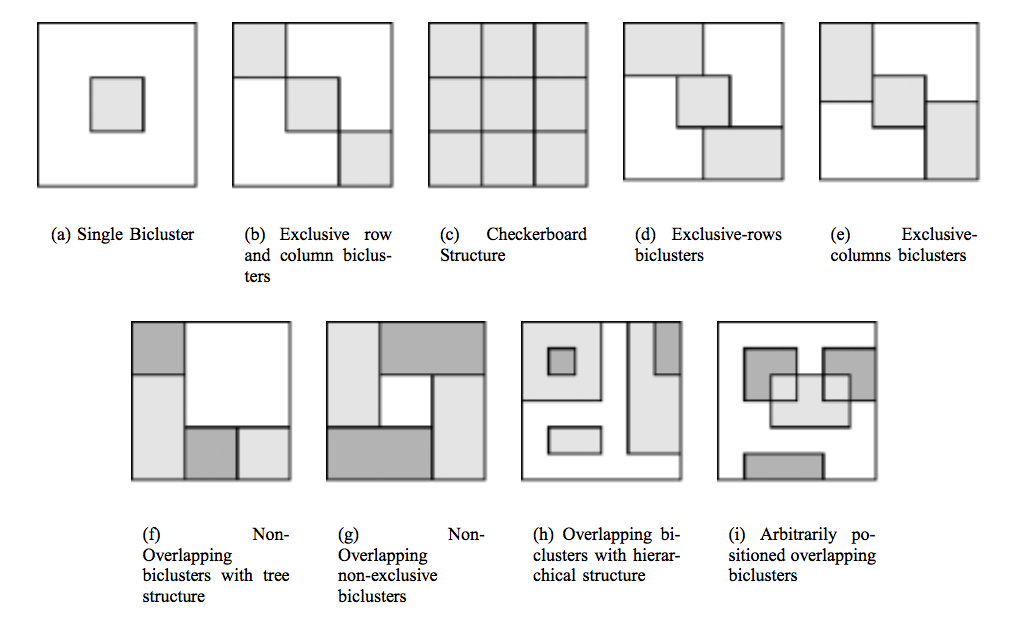
\includegraphics[width=0.7\textwidth]{img/synteticBiclusters.png}
    \label{fig:bicstruct}
\source{\citeonline{Madeira2004}}
\end{figure}

É possível nomear cada uma das estruturas apresentadas na figura~\ref{fig:bicstruct}, considerando as imagens da esquerda para a direita em linha: 1) único cogrupo; 2) cogrupos com linhas e colunas exclusivas; 3) cogrupos com estrutura em xadrez; 4) cogrupos com linhas exclusivas e sobreposição nas colunas; 5) cogrupos com colunas exclusivas e sobreposição nas linhas; 6) cogrupos com estrutura em árvore; 7) cogrupos não exclusivos sem sobreposição; 8) cogrupos com sobreposição e estrutura hierárquica; 9) cogrupos arbitrariamente posicionados.
No capítulo~\ref{ch:experiments} são mostrados experimentos considerando dados sintéticos baseados nessas estruturas, com ênfase nas estruturas que apresentam cogrupos com sobreposição e provendo mais detalhes sobre essas estruturas.

Diversos algoritmos para encontrar cogrupos, de diferentes tipos e estruturas, foram propostos na literatura \cite{Tanay2005,Madeira2004}.

Um dos algoritmos mais simples para a resolução da tarefa de coagrupamento, que é capaz de encontrar cogrupos com valores coerentes em estrutura com sobreposição e arbitrariamente posicionados, é chamado de \textit{Coupled Two-way Clustering} (CTWC)~\cite{Getz2000}.
O algoritmo CTWC é capaz de encontrar cogrupos por meio do agrupamento de dados e atributos (linhas e colunas), separadamente.
\citeonline{Getz2000} utiliza o algoritmo de agrupamento \textit{Superparamagnetic Clustering} (SPC), o qual é capaz de determinar o número de grupos automaticamente com uma estratégia de agrupamento hierárquica.

Já o algoritmo de~\citeonline{Cheng2000} é capaz de encontrar o mesmo tipo de cogrupo que o algoritmo CTWC, porém usando uma estratégia gulosa: cogrupos com valores coerentes e estrutura com sobreposição e arbitrariamente posicionados.
Para encontrar cogrupos, ou $\delta$-cogrupos,~\citeonline{Cheng2000} usam uma estratégia gulosa que retira linhas e colunas de $X$, respeitando um parâmetro $\delta$, que é calibrado pelo usuário.

Além dos algoritmos mencionados, existem outros algoritmos que são capazes de encontrar outros tipos de cogrupos~\cite{Franca20102,Yang2013,Hochreiter2010,Cabanes2012}.

Ainda, de forma semelhante à tarefa de agrupamento, existem métricas de validação que propiciam a avaliação da qualidade e estabilidade de cogrupos, que são separadas em duas das categorias também presentes em agrupamento~\cite{Hochreiter2010}: \textit{interna} e \textit{externa}.
Também, uma das formas de avaliar a qualidade e a estabilidade é pela própria medida de minimização de cada algoritmo, a qual pode não ser tão efetiva quando medidas de validação, mas apresenta-se como uma alternativa.

Resultados de pesquisa apresentados na literatura da área, que fazem uso da visão de coagrupamento discutida, são usados neste trabalho.
Detalhes destes resultados são apresentados, em detalhes, no capítulo~\ref{ch:fatoracao}.

\chapter{Fatoração de matrizes não-negativas para coagrupamento}
\label{ch:fatoracao}

Fatoração de matrizes não-negativas (\textit{Non-negative Matrix Factorization} - NMF) foi estudada como um método para análise de dados capaz de extrair conhecimento sobre um objeto a partir do estudo de suas partes~\cite{lee99}, como um contraponto a métodos mais populares como Análise de Componentes Principais (\textit{Principal Component Analysis - PCA}) e Quantização Vetorial, porém, considerando a fatoração matrizes positivas ou negativas.
\citeonline{lee99} apresentam tal abordagem a partir de sua aplicação no aprendizado de características de faces (em dados do tipo imagem) e na análise de características semânticas de textos.
A análise de textos também foi usada como aplicação na ilustração da aplicação de fatoração de matrizes por~\citeonline{Ho2008} que segue a ideia de aprendizado de partes, por~\citeonline{Kuang2014} que aplica fatoração de matrizes não-negativas sobre um problema formulado como análise de agrupamento (clustering), e por~\citeonline{Long2005, Ding06, Yoo2010}, que formulam o problema como coagrupamento.
Ainda, outros contextos são submetidos à análise sob a formulação de problemas de coagrupamento, sendo alguns exemplos o agrupamento de genes e análise de microarray em bioinformática~\cite{Kluger2003}, e a filtragem colaborativa em sistemas de recomendação~\cite{SalMnih08}.
Na aplicação de NMF em filtragem colaborativa em sistemas de recomendação, destaca-se o modelo baseado em NMF de~\citeonline{Koren09} para predição de preferências de usuários por filmes, que ganhou o Prêmio Netflix (\textit{Netflix Prize})\footnote{\url{http://www.netflixprize.com/}} em primeiro lugar.

A adequação da fatoração de matrizes para tarefas modeladas como agrupamento ou coagrupamento ocorre porque muitas das representações usadas em aplicações nessas áreas se apresentam como uma relação entre pares de elementos pertencentes a conjuntos finitos, como apresentado em \cite{Long2005}. Por exemplo, na resolução da tarefa de agrupamento de documentos, em mineração de texto, usa-se, comumente, dois conjuntos finitos, documentos e palavras, sendo que a relação entre eles é representada pela ocorrência de uma determinada palavra em um determinado documento. Note ainda que a relação expressa entre os elementos, como no contexto de palavras e documentos, apresenta-se como uma matriz de dados positiva, característica que ilustra a aplicabilidade de NMF.

Formalmente, algoritmos de coagrupamento baseados em NMF têm como entrada uma matriz de dados $X \in \mathbb{R}^{n \times m}_{+}$, contendo números reais positivos com $n$ linhas e $m$ colunas.
Esta matriz é formada por um conjunto de vetores de linhas $\mathcal{N} = \{ \mathbf{x}_{1 \cdot}, \dots, \mathbf{x}_{n \cdot} \}$ e um conjunto de vetores de colunas $\mathcal{M} = \{ \mathbf{x}_{\cdot 1}, \dots, \mathbf{x}_{\cdot m} \}$, e as relações existentes entre cada linha $\mathbf{x}_{i \cdot}$ e cada coluna $\mathbf{x}_{\cdot j}$ são representadas por $x_{ij}$ considerando os índices $i \in \{1, \dots, n\}$ e $j \in \{1, \dots, m\}$, que é justamente um valor da matriz $X$.
Cada valor em $x_{ij}$ representa, então, a relação existente entre pares de elementos em algum contexto de interesse.
O objetivo é encontrar $k$ partições de $\mathcal{N}$, denotadas pelos subconjuntos ordenados $\mathcal{K}_p \subseteq \mathcal{N}$, $l$ partições para $\mathcal{M}$, denotadas pelos subconjuntos ordenados $\mathcal{L}_q \subseteq \mathcal{M}$, considerando os índices $p \in \{ 1, \dots, k\}$ e $q \in \{1, \dots, l\}$.
Então, os conjuntos $\{\mathcal{K}_1, \dots, \mathcal{K}_k\}$ e $\{\mathcal{L}_1, \dots, \mathcal{L}_l\}$ são os cogrupos de linhas e colunas, respectivamente.
Da mesma forma que na tarefa de agrupamento, faz-se sentido a proposição de algoritmos baseados em heurísticas, pois sob diversas formas, o problema de coagrupamento baseado em particionamento, é um problema NP-difícil~\cite{Bulteau2014}.

% Não sei se entendi bem, mas mudei o texto para colocar como partições. Sobre a questão da forma de representa X e Y, posso estar falando besteira, mas me parece que tanto faz de um jeito o de outro, visto que o que tem dentro de partições de linhas e colunas são linhas e colunas. Eu só estou um pouco receosa de chamar de vetores de colunas. Em clustering a notação para as linhas é essa, mas lá não faz sentido chamar de vetores de colunas.

%%% comentário do Valdinei: Como escrevi anteriormente, prefiro dizer que $\mathcal{N}=\{1,2,\dots,n\}$ e o mesmo para $\mathcal{M}$, então faz mais sentido formar os cogrupos com $I\subseteq\mathcal{N}$ e o mesmo para $J$. Além disso, os índices $p$ e $q$ não foram mencionados. Finalmente, aqui já está considerando que os clusters de linha são separados dos cluster de colunas, como é utilizado tradicionalmente na literatura. Dessa forma, deve-se dizer que os conjuntos $I$ devem formar uma partição de $\mathcal{N}$.)}

Para implementação da NMF como uma estratégia para resolução do problema de coagruamento, diferentes algoritmos foram apresentados na literatura.
Cada um deles considera o problema de NMF com diferentes restrições que permitem propor soluções para o problema de coagrupamento de diferentes naturezas.
Este capítulo se destina a apresentar três das implementações existentes que são usadas como base para a proposta desta dissertação: decomposição de valores em blocos (Seção~\ref{sec:bvd}) introduzida por~\citeonline{Long2005}; fatoração ortogonal tripla de matrizes não-negativas (Seção~\ref{sec:ONMTF}) introduzida por~\citeonline{Ding06}; e fatoração tripla rápida de matrizes não-negativas (Seção~\ref{sec:FNMTF}) introduzida por~\citeonline{Wang2011}.
Outras implementações correlatas podem ser encontradas em~\cite{Li2006}.

Todos algoritmos de NMF para resolução das tarefas de agrupamento e coagrupamento tem em comum a natureza recursiva, pois são encontradas partições de linhas a partir de partições de colunas, para então, encontrar melhores partições de colunas a partir das partições de linhas.
Esse processo recursivo continua até que a aproximação entre a fatoração e a matriz fatorada ($X$), através de alguma medida, atinja um mínimo local ou global, resultando em uma solução para o particionamento de linhas e colunas.

\section{Decomposição de Valores em Blocos para Coagrupamento}
\label{sec:bvd}

A Decomposição de Valores em Blocos (\textit{Block Value Decomposition} - \textit{BVD}) foi proposta por~\citeonline{Long2005} como uma abordagem para tratar o problema de coagrupamento, com base em fatoração de matrizes não-negativas.
Essa decomposição recebe esse nome por ter a capacidade de encontrar estruturas em blocos escondidas na matriz de dados.
Isso é possível porque o algoritmo \textit{BVD} é capaz de explorar a relação entre linhas e colunas da matriz de dados por meio da decomposição dela em três matrizes: $U$ uma matriz de coeficientes de linhas, $S$ uma matriz com estrutura em blocos, e $V$ uma matriz de coeficientes de colunas.
Segundo os autores, tais coeficientes em $U$ e $V$ podem ser vistos como um fator que associa linhas à partições encontradas no conjunto de linhas, e que associa as colunas à partições encontradas no conjunto de colunas, respectivamente; e $S$ pode ser vista como a representação média dos detalhes da matriz original e permite sua reconstrução aproximada a partir da operação $USV^T$.
Sob o ponto de vista da resolução do problema de coagrupamento, então, o objetivo no \textit{BVD} é encontrar grupos de linhas e colunas de forma simultânea, sendo $k$ grupos de $\mathcal{N}$ (linhas) e $l$ grupos de $\mathcal{M}$ (colunas).

Ainda, os autores proponentes da abordagem \textit{BVD} defendem que interpretações intuitivas podem ser derivadas da análise das combinações das matrizes geradas na fatoração, quando aplicadas a um contexto específico.
Um exemplo fornecido no trabalho de \citeonline{Long2005} é que, considerando uma matriz de entrada que representa a relação ``documentos por palavras'' (linhas por colunas) cada coluna de $US$ captura a ideia de uma base para a representação de grupos de palavras; e cada linha em $SV^T$ captura a ideia de uma base para a representação de grupos de documentos.
Uma representação gráfica para o resultado de uma fatoração de matrizes pode ser vista na figura~\ref{fig:bvd}.

% tentei deixar menos associado à S e mais genérico, independente de S - exatamente como estava no artigo original. Talvez tenha melhorado.4
% Obeservação do Valdinei: Parece que aqui é a primeira vez aparece "características" e "objetos", essa interpretação da matriz tem que ser dada mais força anteriormente.
% Além disso, essa interpretação da matriz $S$ não me convence muito. Se restringirmos as matrizes $U$ e $V$ a serem binárias, a interpretação de $S$ fica sendo o valor de $\mu$ comentado no capítulo de "Tipos de Cocluster".)}

% TODO explicar melhor as figuras
\begin{figure}[H]
\centering
\caption{
Fatoração da matriz original de dados $X$ em três outras matrizes: $U$, $S$ e $V$}
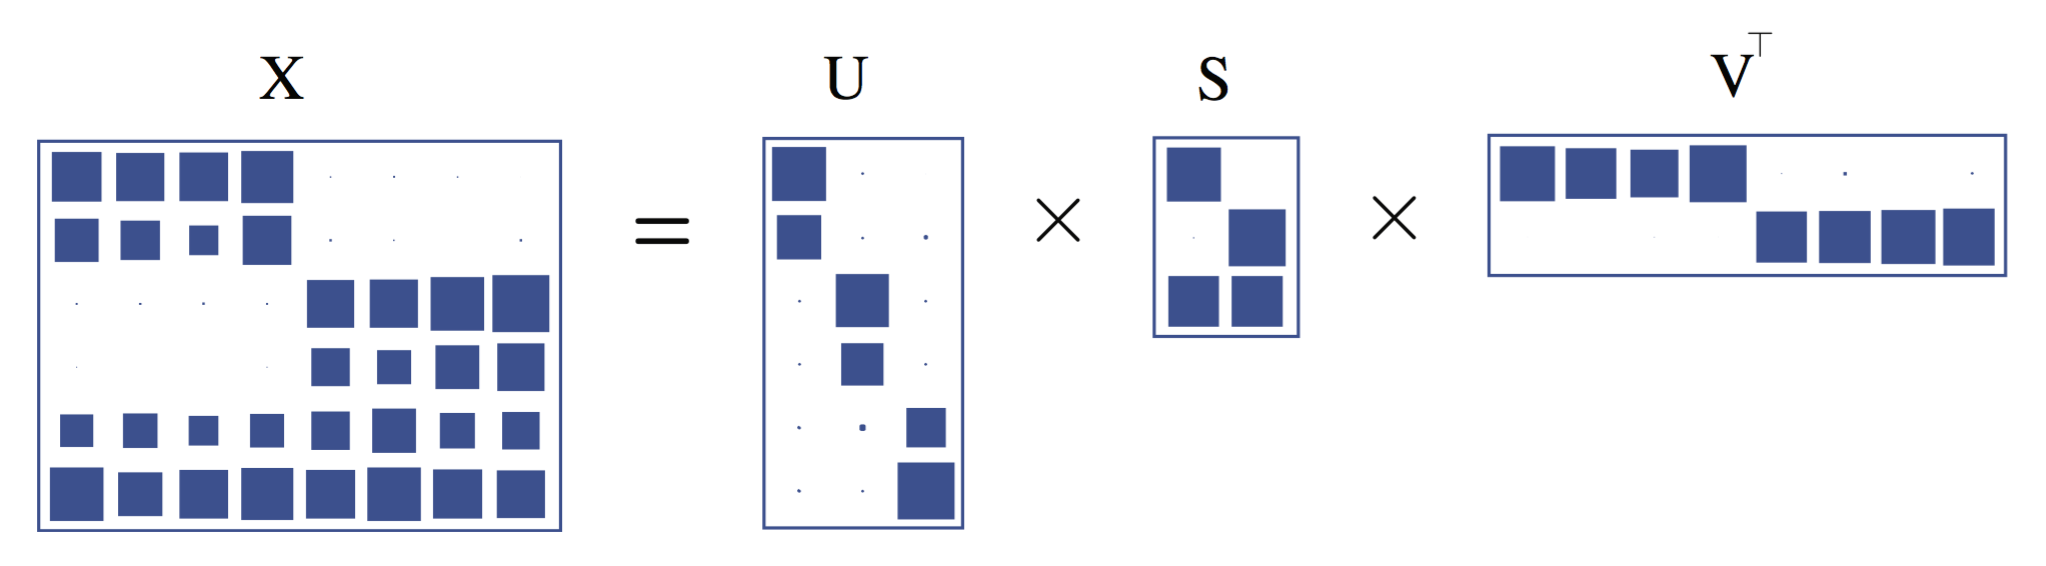
\includegraphics[width=0.6\textwidth]{img/factorizationXUSV.png}
\label{fig:bvd}
\source{Adaptado de \citeonline{Yoo2010}}
\end{figure}

Na figura~\ref{fig:bvd} considere que uma célula com cor escura representa a existência de uma relação entre linha e coluna, e uma célula com cor clara representa a inexistência de uma relação entre linha e coluna, e que essas relações são estabelecidas adequadamente em cada contexto de aplicação.
Transportando o exemplo da figura para o contexto de uma matriz de ``documentos por palavras'' tem-se um conjunto de seis documentos e quatro palavras, sendo que, por exemplo, o primeiro documento possui uma relação com as duas primeiras palavras, e não possui relação com as terceira e quarta palavras.
A matriz $U$ pode ser interpretada como uma matriz ``documentos por grupos de documentos'', sendo portanto uma situação em que seis documentos estão agrupados em três grupos ($k = 3$): os dois primeiros documentos no primeiro grupo, os dois próximos no segundo grupo e os dois últimos no terceiro grupo.
A matriz $V^T$ pode ser interpretada como uma matriz de ``grupos de palavras por palavras'', sendo portanto uma situação em que há dois grupos de palavras ($l = 2$) no contexto das quatro palavras existentes.
Finalmente, a matriz $S$ representa uma relação entre ``grupos de documentos'' e ``grupos de palavras''.
A primeira linha da matriz $S$ indica que há uma relação entre o primeiro grupo de linhas e o primeiro grupos de palavras, e que não há uma relação entre o primeiro grupo de linhas e o segundo grupo de palavras.
Seguindo a interpretação intuitiva apresentada por \cite{Long2005}, uma das combinações possíveis, $SV^T$, está ilustrada na figura~\ref{fig:bvd:reconstruction}.
Observe que a matriz $SV^T$ representa ``três grupos de documentos por quatro palavras'', constituindo-se como uma base de representação para grupos de documentos.

Note ainda que nessa estrutura de matrizes fatoradas é possível identificar protótipos responsáveis por cada parte da reconstrução da matriz original $X$, visto que cada base de representação pode ser vista como um conjunto de vetores protótipos: as linhas de $(SV^T)$ são vetores base (protótipos de grupos de linhas).
O raciocínio apresentado para interpretação da figura~\ref{fig:bvd:reconstruction} pode também ser feito para a interpretação da combinação $US$.
Importante salientar que, assim como ocorre na resolução da tarefa de agrupamento, diferentes grupos de linhas e de colunas podem ser obtidos, representando diferentes soluções para o problema.
E, neste caso ainda, diferentes matrizes $S$ podem ser obtidas para uma mesma organização de grupos de linhas e colunas.
Portanto, qualquer interpretação derivada dessa análise deve ser considerada como apenas uma das formas possíveis de análise dos dados provenientes do contexto de aplicação.

\begin{figure}[H]
\centering
\caption{
A reconstrução da primeira linha $\mathbf{x}_{1 \cdot}$ de $X$, através da multiplicação da matriz indicadora de grupos de linhas $U$ pela matriz dos protótipos de linhas $(S V^T)$. %que para a primeira linha seleciona apenas o primeiro protótipo,
}
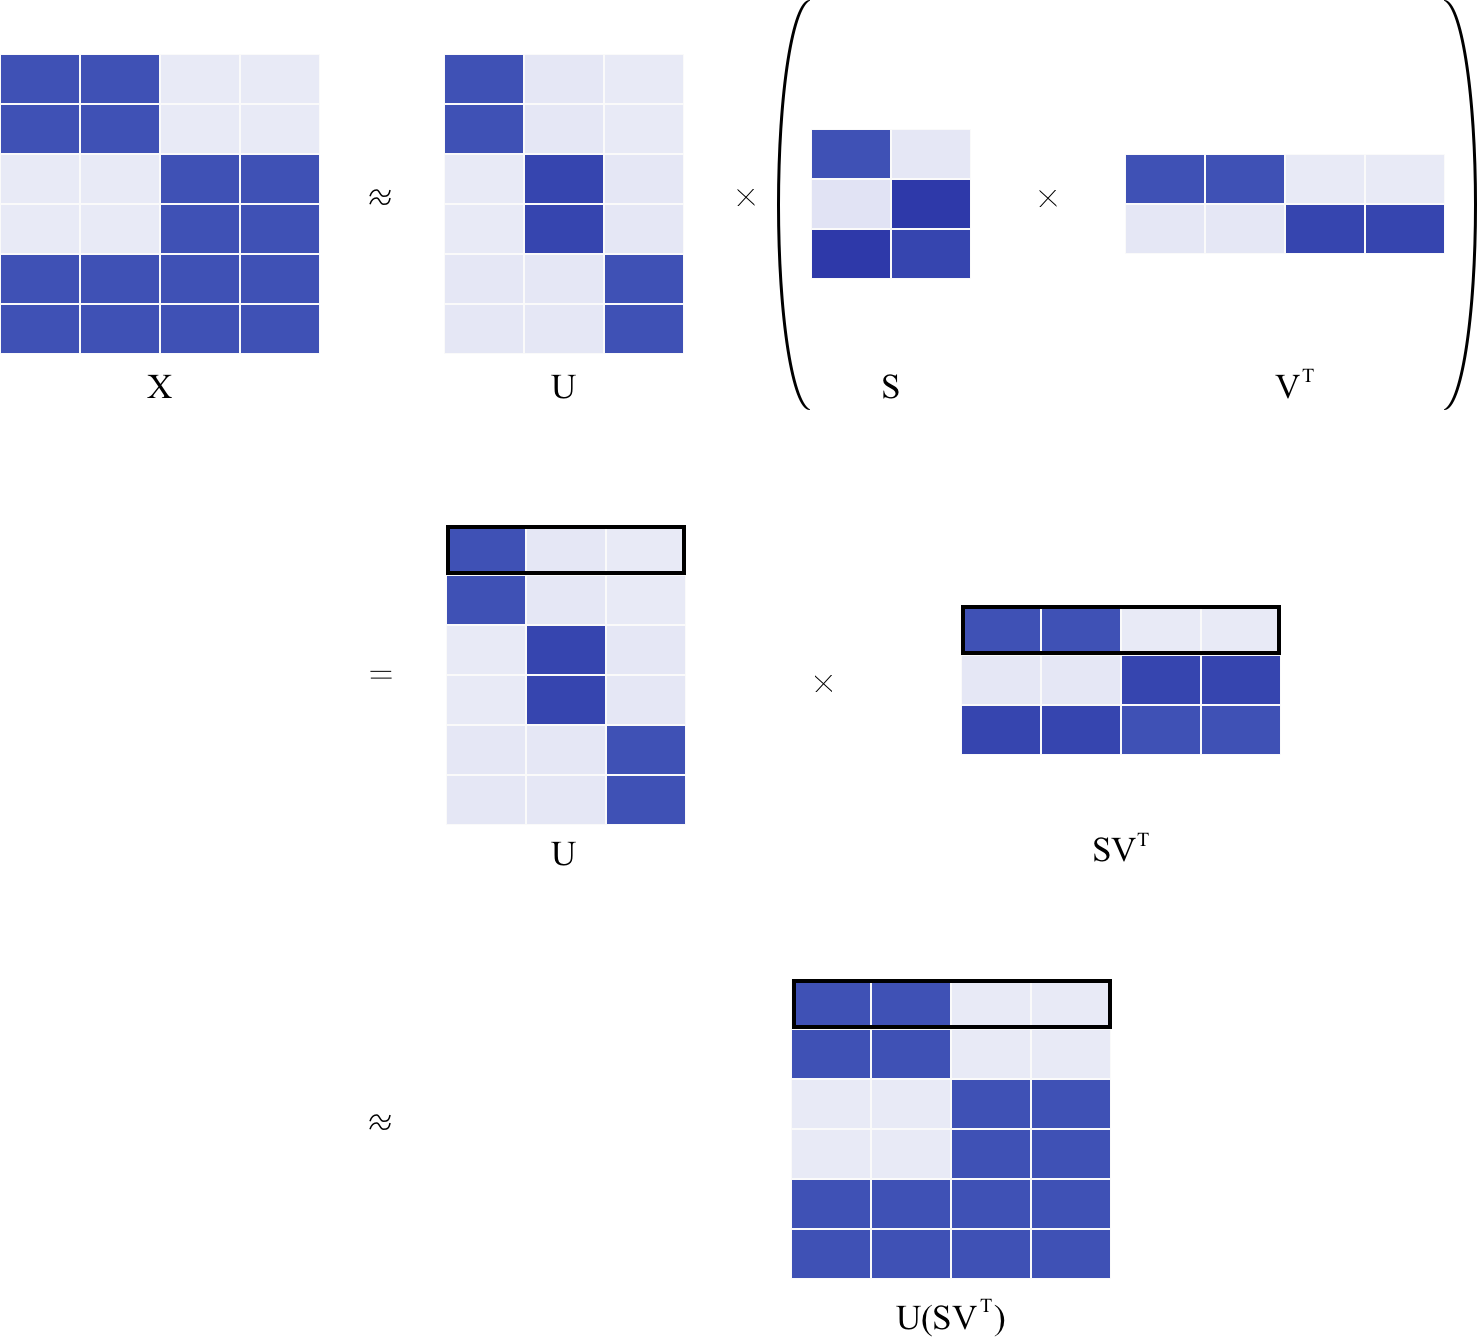
\includegraphics[width=0.6\textwidth]{img/reconstruction.png}
\label{fig:bvd:reconstruction}
\source{Lucas Fernandes Brunialti, 2016}
\end{figure}

Semelhante ao \textit{fuzzy k-means}, é possível observar esta fatoração como uma ótica de compactação.
O \textit{BVD} compacta a matriz de dados em uma matriz com fatores que correlacionam cada linha com cada grupo de linhas ($U$).
Além disso, esta compactação adiciona a idéia de uma matriz de fatores $V$ para compactar as colunas de $X$, e $S$ que é uma visão compactada de $X$ em $kl$ elementos.
Portanto, a compactação transforma $nm$ elementos em $nk + kl + ml$ elementos, através das matrizes $U$, $S$ e $V$, e supondo que $n \ll k$ e $m \ll l$, tem-se que $mm \ll nk + kl + ml$.

O problema de coagrupamento implementado sob a abordagem \textit{BVD} é formalmente apresentado como \cite{Long2005}:

\begin{problem}[Problema de decomposição de valores em blocos]
\label{def:bvd:problem}
    \begin{equation}
        \begin{array}{lclcl}
            \displaystyle \mathcal{F}_3(U, S, V) & = & \displaystyle \min_{U, S, V} & \norm{X - USV^T}^{2}_{F} \\
                                               &   & \text{suj. a}                & U \geq 0,                  \\
                                               &   &                              & S \geq 0,                  \\
                                               &   &                              & V \geq 0
        \end{array}   \nonumber
    \end{equation}
em que $U \in \mathbb{R}^{n \times k}_{+}$, $S \in \mathbb{R}^{k \times l}_{+}$, $V \in \mathbb{R}^{m \times l}$, e $\norm{\cdot}_F$ denota a norma de Frobenius para matrizes.
\end{problem}

%% *******************************************************************************************************
%% *******************************************************************************************************
%% *******************************************************************************************************
%% Bom, entendi que essa parte de Lagrange é para provar que o problema vai convergir, então por enquanto comentei visto que nós não vamos fazer provas nos outros algoritmos. Se não for para tirar, voltamos. Como entendi que era para tirar, não li.
%
%Introduzindo a função lagrangeana, associada à $\mathcal{F}_1$:
%\[
%    \displaystyle \mathcal{L}(U, S, V, \Lambda_1, \Lambda_2, \Lambda_3) = \norm{X - USV^T}^{2}_{F} - tr(\Lambda_1 U^T) - tr(\Lambda_2 S^T) - tr(\Lambda_3 V^T) \\
%\]
%
%onde $\Lambda_1 \in \mathbb{R}^{n \times k}$, $\Lambda_2 \in \mathbb{R}^{k \times l}$ e $\Lambda_3 \in \mathbb{R}^{m \times l}$ são os multiplicadores de Lagrange.
%
%Pela teoria de otimização não-linear com restrições, $\Theta = (U^{*}, S^{*}, V^{*}, \Lambda_{1}^*, \Lambda_{2}^*, \Lambda_{3}^*)$ será um mínimo local estacionário de $\mathcal{F}_1$, se e somente se, respeitar as condições de regularidade de \textit{Karush-Kuhn-Tucker} (KKT)~\cite{bazaraa2006}:
%
%\begin{subequations}
%    \begin{alignat}{3}
%        U^* \geq 0, \quad                  && S^* \geq 0, \quad                     && V^* \geq 0                  \label{eq:bvd:kkt1} \\
%        \quad                              && \nabla_{\Theta} \mathcal{L} = 0 \quad &&                             \label{eq:bvd:kkt2} \\
%        \Lambda_{1}^* \odot U^* = 0, \quad && \Lambda_{2}^* \odot S^* = 0, \quad    && \Lambda_{3}^* \odot V^* = 0 \label{eq:bvd:kkt3}
%    \end{alignat}
%\end{subequations}
%
%onde $\odot$ denota o produto de Hadamard.
%
%É possível expandir as equações em~\ref{eq:bvd:kkt2}, calculando as derivadas:
%
%\[
%\begin{array}{lclclclcl}
%    \nabla_U \mathcal{L} & = & U S V^{T} V S^{T}     & - & X V^{T} S^{T} & - & \Lambda_1 & = & 0 \\
%    \nabla_S \mathcal{L} & = & U^{T} U S V^{T} V     & - & U^{T} X V     & - & \Lambda_2 & = & 0 \\
%    \nabla_V \mathcal{L} & = & S^{T} U^{T} U S V^{T} & - & S^{T} U^{T} X & - & \Lambda_3 & = & 0
%\end{array}
%\]
%
%Aplicando o produto Hadamard dos dois lados de cada uma das equações e utilizando das condições em~\ref{eq:bvd:kkt3}:
%\[
%\begin{array}{lclclclclcl}
%    \nabla_U \mathcal{L} & = & U & \odot & U S V^{T} V S^{T}     & - & U & \odot & X V^{T} S^{T} & = & 0 \\
%    \nabla_S \mathcal{L} & = & S & \odot & U^{T} U S V^{T} V     & - & S & \odot & U^{T} X V     & = & 0 \\
%    \nabla_V \mathcal{L} & = & V & \odot & S^{T} U^{T} U S V^{T} & - & V & \odot & S^{T} U^{T} X & = & 0
%\end{array}
%\]
%
%Desta forma, é possível resolver para $U$ de forma algébrica:
%\[
%\begin{array}{lclclcl}
%             & U \odot U S V^{T} V S^{T}                           & = & U \odot X V^{T} S^{T} \\
%    \implies & U \odot \frac{U S V^{T} V S^{T}}{U S V^{T} V S^{T}} & = & U \odot \frac{X V^{T} S^{T}}{U S V^{T} V S^{T}}
%\end{array}
%\]
%
%\[
%    \begin{array}{lclcl}
%        \therefore & U & = & U \odot \frac{X V^{T} S^{T}}{U S V^{T} V S^{T}}
%    \end{array}
%\]
%
%% *******************************************************************************************************
%% *******************************************************************************************************
%% *******************************************************************************************************

A implementação para o processo de minimização do problema~\ref{def:bvd:problem} é descrito no algoritmo~\ref{algo:bvd}, o qual é baseado em atualizações multiplicativas e tem sua convergência demonstrada via teoria de otimização não linear (veja \citeonline{Long2005}).
Nesse algoritmo considere $t$ o contador de iterações, e $U^{(t)}$, $S^{(t)}$ e $V^{(t)}$, as matrizes $U$, $S$ e $V$, na iteração $t$, respectivamente.
% Sara: ué gente, porque t+1 para iteração atual em S e V ????
% Sara: essa ordem de alteração das matrizes está correta??? No artigo não é essa, mas lá não entendi que ele dá a ordem. De onde veio a ordem?

% Lucas: Esse é o mistério, ninguém comenta muito sobre isso, mas na prática só funciona assim, quer dizer, do outro jeito "funciona" tbm, mas a medida de aproximação fica meio louca. A minha idéia é que é assim pq a otimização é alternada, primeiro otimiza pra U fixando S e V, melhora a solução de U, otimiza pra V fixando S e V, melhora a solução de V, otimiza pra S fixando U e V, melhora a solução de S. O mais bizarro é que se foge dessa ordem, a medida de aproximação fica louca.

\begin{algorithm}
\caption{Algoritmo baseado em atualização multiplicativa para solução do \textit{BVD}}
\label{algo:bvd}
\begin{algorithmic}[1]
\Function{BVD}{$X$, $k$, $l$, $t_{max}$}
\State \textbf{Inicialize:} $U^{(0)} \gets \mathcal{U}(0, 1), V^{(0)} \gets \mathcal{U}(0, 1), S^{(0)} \gets \frac{1}{nm} \sum_{i, j} x_{ij}$ e $t \gets 0$.
\While{(não convergiu) e ($t \leq t_{max}$)} %\Comment{We have the answer if r is 0}
\State
\begin{equation}
\label{eq:bvd:updateU}
U^{(t+1)} \gets U^{(t)} \odot \frac{ X V^{(t)} S^{(t)^T} }{ U^{(t)} S^{(t)} V^{(t)^T} V^{(t)} S^{(t)^T }}             \nonumber
\end{equation}
\State
\begin{equation}
\label{eq:bvd:updateV}
V^{(t+1)} \gets V^{(t)} \odot \frac{ X^T U^{(t+1)} S^{(t)} }{ V^{(t)} S^{(t)^T} U^{(t+1)^T} U^{(t+1)} S^{(t)} }       \nonumber
\end{equation}
\State
\begin{equation}
\label{eq:bvd:updateS}
S^{(t+1)} \gets S^{(t)} \odot \frac{ U^{(t+1)^T} X V^{(t+1)} }{ U^{(t+1)^T} U^{(t+1)} S^{(t)} V^{(t+1)^T} V^{(t+1)} } \nonumber
\end{equation}
\State $t \gets t + 1$
\EndWhile\label{euclidendwhile}
\State \textbf{return} $U^{(t)}, S^{(t)}, V^{(t)}$
\EndFunction
\end{algorithmic}
\end{algorithm}

A inicialização dos elementos das matrizes $U$, $S$ e $V$ são gerados através de uma distribuição uniforme ($\mathcal{U}(0, 1) \in~]0, 1]$).
Como condições para assumir a convergência, neste trabalho, considera-se a diferença do erro de aproximação em duas iterações consecutivas menor ou igual a um $\epsilon$:
$$\norm{X - U^{(t)} S^{(t)} V^{(t)^T}}^{2}_{F} - \norm{X - U^{(t+1)} S^{(t+1)} V^{(t+1)^T}}^{2}_{F} \leq \epsilon$$
O algoritmo também pára caso a quantidade de iterações assuma o limite $t_{max}$.

Note que como $U$ e $V$ possuem valores no domínio dos reais, então, não é possível obter as partições diretamente, sem um processo de pós-processamento.
Um modo simples de obter o particionamento para as linhas toma a seguinte forma:
$$\mathcal{K}_{p}=\{x_{i\cdot}~|~i\in\{1,\dots,n\}\text{ e }p=\argmax_{p'\in\{1,\dots,k\}} u_{ip'} \}, \forall p\in\{1,\dots,k\}$$

Isso significa que uma linha $i$ pertencerá a um cogrupo $p$ (ou partição) se para todos os $k$ cogrupos, o fator $u_{ip}$ for maior que todos os outros fatores para os outros cogrupos, presentes no vetor $\mathbf{u}_{i \cdot}$.

A complexidade de tempo do algoritmo é possível ser calculada fixando as condições $k \simeq l$, $n \simeq m$, $k \ll n$, $l \ll m$ e usando um algoritmo para otimizar a ordem das multiplicações (\citeonline{Cormen2001} discute algoritmos para tal otimização): $\mathcal{O}\Big( t_{max} \big( nl (m + k) + ml (n + k) + mk (n + l) + k^2 (n + l) + l^2 (m + k) \big) \Big) \simeq \mathcal{O}\Big( t_{max} \big( n^2k + nk^2 + k^3 ) \Big)$.


% \begin{theorem}[Corretude]
% \label{def:bvd:correctness}
%     As regras de atualização das equações~\ref{eq:bvd:updateU},~\ref{eq:bvd:updateV} e~\ref{eq:bvd:updateS} são corretas para resolução do problema~\ref{def:bvd:problem}, ou seja, respeitam a condição da equação~\ref{eq:bvd:kkt2}.
% \end{theorem}

% \begin{proof}
%     Esse algoritmo usa o método de iteração de ponto fixo, então, para $U$, se \linebreak
%      $U^{(t)} S^{(t)} V^{(t)^T} V^{(t)} S^{(t)^T} \neq 0$ e $U^{(t + 1)} = U^t \geq 0$, então:
%     \[
%         X V^{(t)^T} S^{(t)^T} = U^{(t)} S^{(t)} V^{(t)^T} V^{(t)} S^{(t)^T} \Rightarrow \nabla_U \mathcal{L} = 0
%     \]
%     verificando a condição da equação~\ref{eq:bvd:kkt2}. O mesmo processo pode ser realizado para $S$ e $V$.
% \end{proof}

% \begin{theorem}[Convergência]
% \label{def:bvd:convergence}
%     O problema~\ref{def:bvd:problem} é decrescente sob as regras de atualização das equações~\ref{eq:bvd:updateU},~\ref{eq:bvd:updateV} e~\ref{eq:bvd:updateS}.
% \end{theorem}

% \begin{proof}
%     % Fixa S e V 1o?
%     Seja uma função auxiliar $G(U)$ para $F(U)$.
% \end{proof}

\section{Fatoração Ortogonal Tripla de Matrizes Não-negativas}
\label{sec:ONMTF}

Baseado no problema~\ref{def:bvd:problem}, \citeonline{Ding06} propõem o problema~\ref{def:onmtf:problem}, e o chama de Fatoração Ortogonal Tripla de Matrizes Não-negativas (\textit{Orthogonal Non-negative Matrix Tri-factorization} - \textit{ONMTF}).

\begin{problem}[Problema de fatoração ortogonal tripla de matrizes não-negativas]
\label{def:onmtf:problem}
\begin{equation}
    \begin{array}{lclcl}
        \displaystyle \mathcal{F}_6(U, S, V) & = & \displaystyle \min_{U, S, V} & \norm{X - USV^T}^{2}_{F}      \\
                                             &   & \text{suj. a}                & U \geq 0, S \geq 0, V \geq 0, \\
                                             &   &                              & U^T U = I,                    \\
                                             &   &                              & V^T V = I
    \end{array}   \nonumber
\end{equation}
em que $U \in \mathbb{R}^{n \times k}_{+}$, $S \in \mathbb{R}^{k \times l}_{+}$, $V \in \mathbb{R}^{m \times l}_{+}$ e $\norm{\cdot}_F$ denota a norma de Frobenius.
\end{problem}

Na formulação desse problema, duas restrições de ortonormalidade são acrescentadas, $U^T U = I$ e $V^T V = I$, em que $I$ é a matriz identidade, para as matrizes de grupos de linhas e grupos de colunas, respectivamente.
Tais restrições restringem o problema da fatoração $X \approx USV^T$ para um número menor de possíveis soluções, buscando a unicidade, como mostrado na figura~\ref{fig:bvdvsonmtf}.
No entanto, o algoritmo não garante que as restrições de ortonomalidade são respeitadas, apesar das restrições colocadas encontrarem soluções de particionamento com maior ortogonalidade.

% $U \geq 0, S \geq 0, V \geq 0$ sendo todos os elementos de $U$, $S$ e $V$, maior que $0$, respectivamente, $U^T U = I$ e $V^T V = I$ as restrições de ortonomalidade para as matrizes indicadoras de grupos de linhas e colunas, respectivamente, e $\norm{\cdot}_F$ denota a norma de Frobenius para matrizes.

\begin{figure} [htpb]
\centering
\caption{Base de protótipos obtidas com NMF sem restrições (a) e com restrições de ortogonalidade nas matrizes}
\begin{subfigure}[b]{0.3\textwidth}
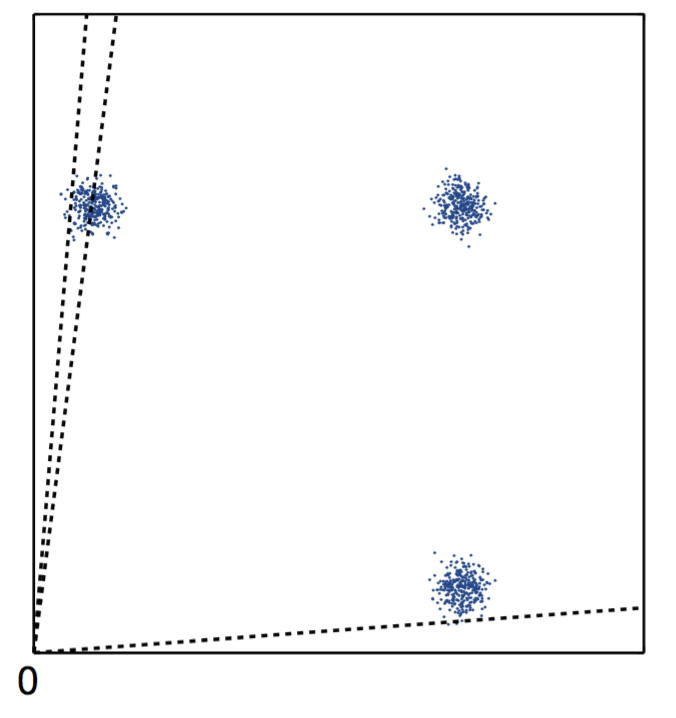
\includegraphics[width=\textwidth]{img/bvdVsOnmtf1.png}
\caption{}
\label{fig:bvdvsonmtf:1}
\end{subfigure}
~ %add desired spacing between images, e. g. ~, \quad, \qquad, \hfill etc.
%(or a blank line to force the subfigure onto a new line)
\begin{subfigure}[b]{0.3\textwidth}
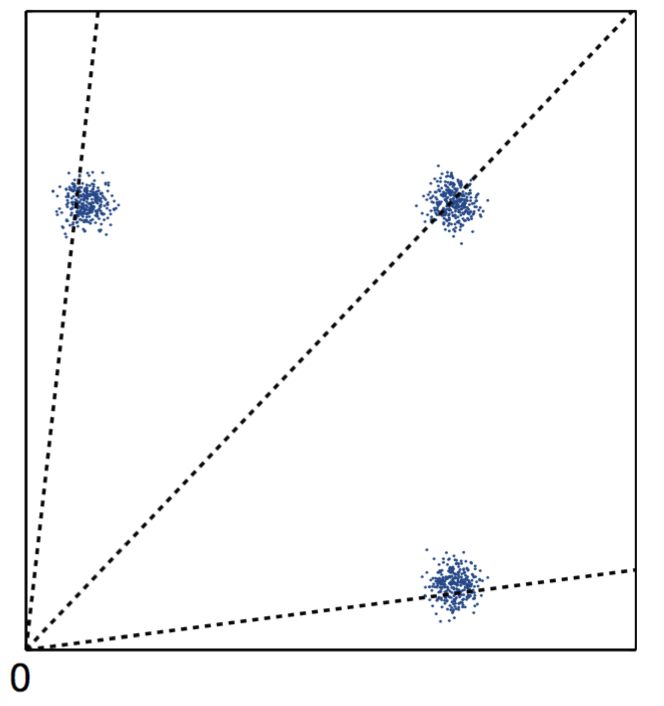
\includegraphics[width=\textwidth]{img/bvdVsOnmtf2.png}
\caption{}
\label{fig:bvdvsonmtf:2}
\end{subfigure}

%       Um exemplo sintético que compara o algoritmo para \textit{BVD} contra o algoritmo para ONMTF, com pontos sendo dados, as linhas pontilhadas sendo os protótipos de linhas ($S V^T$), e os três conjuntos de pontos sendo os grupos. (a) O algoritmo para \textit{BVD} encontra uma solução com dois protótipos em um mesmo grupo, deixando um dos grupos sem nenhum protótipo para representá-lo. Apesar de ser uma solução correta, ou seja, encontra um mínimo local, não é a desejada. (b) O algoritmo para ONMTF é capaz de encontrar a solução em que cada protótipo aproxima cada grupo de dados, através das restrições referentes à ortogonalidade, este é capaz de restringir as possíveis soluções para a fatoração $X \approx U S V^T$.

\label{fig:bvdvsonmtf}
\source{\citeonline{Yoo2010}}
\end{figure}

A figura~\ref{fig:bvdvsonmtf} representa um problema com três grupos (três nuvens de pontos).
As linhas pontilhadas representam os protótipos obtidos por NMF (a) sem restrição de ortogonalidade nas matrizes, como o \textit{BVD}, e (b) com restrição de ortogonalidade nas matrizes, como o \textit{ONMTF}.
Note que a base obtida com NMF ortogonal tende a encontrar protótipos mais centralizados nos grupos.
Já a base obtida com NMF sem restrições tende a encontrar uma região convexa que contém os pontos dos grupos (incluindo regiões que abrangem pontos de grupos originalmente projetados como sendo diferentes).
A solução obtida em (a), embora correta, não é desejável.

Em termos de compactação, igualmente ao \textit{BVD}, o algoritmo para solução do \textit{ONMTF} transforma os $nm$ elementos da matriz $X$ em $nk + kl + ml$ elementos, através da fatoração em $U$, $S$ e $V$, e supondo que $n \ll k$ e $m \ll l$, tem-se que $mm \ll nk + kl + ml$.

\citeonline{Ding06} propõem uma solução para implementação do processo de minimização para o problema~\ref{def:onmtf:problem} semelhante ao que foi apresentado na seção~\ref{sec:bvd}, também baseado em atualizações multiplicativas e com convergência demonstrada com base na teoria de otimização não-linear.
O algoritmo para tal processo de minimização é apresentado no algoritmo~\ref{algo:onmtf}, no qual $t$ é o contador de iterações, $U^{(t)}$, $S^{(t)}$ e $V^{(t)}$, as matrizes $U$, $S$ e $V$ na iteração $t$, respectivamente, e $\mathcal{U}(0, 1) \in~]0, 1]$ uma função que gera valores de uma distribuição uniforme.
Também, a mesma condição de convergência aplicada no algoritmo~\ref{algo:bvd} pode ser aplicada nesse caso.

%fazendo a derivação através da função lagrangeana e a introdução dos multiplicadores de lagrange, utilizando as condições de otimização não-linear de KKT, derivando as regras para atualização multiplicativa para $U$, $S$ e $V$, apresentadas no algoritmo~\ref{algo:onmtf}.

\begin{algorithm}
\caption{Algoritmo baseado em atualização multiplicativa para solução do \textit{ONMTF}}
\label{algo:onmtf}
\begin{algorithmic}[1]
\Function{ONM3F}{$X$, $k$, $l$, $t_{max}$}
\State \textbf{Inicialize:} $U^{(0)} \gets \mathcal{U}(0, 1), V^{(0)} \gets \mathcal{U}(0, 1), S^{(0)} \gets \mathcal{U}(0, 1)$ e $t \gets 0$.
\While{(não convergiu) e ($t \leq t_{max}$)} %\Comment{We have the answer if r is 0}
\State
\begin{equation}
\label{eq:onmtf:updateU}
U^{(t+1)} \gets U^{(t)} \odot \sqrt{ \frac{ X V^{(t)} S^{(t)^T} }{ U^{(t)} U^{(t)^T} X V^{(t)} S^{(t)^T} } }
\end{equation}
\State
\begin{equation}
\label{eq:onmtf:updateV}
V^{(t+1)} \gets V^{(t)} \odot \sqrt{ \frac{ X^T U^{(t+1)} S }{ V^{(t)} V^{(t)^T} X^T U^{(t+1)} S^{(t)} } }
\end{equation}
\State
\begin{equation}
\label{eq:onmtf:updateS}
S^{(t+1)} \gets S^{(t)} \odot \sqrt{ \frac{ U^{(t+1)^T} X V^{(t+1)} }{ U^{(t+1)^T} U^{(t+1)} S^{(t)} V^{(t+1)^T} V^{(t+1)} } }
\end{equation}
\State $t \gets t + 1$
\EndWhile\label{euclidendwhile}
\State \textbf{return} $U^{(t)}, S^{(t)}, V^{(t)}$
\EndFunction
\end{algorithmic}
\end{algorithm}

Note que é possível obter o particionamento de linhas e colunas da mesma forma que foi descrita com o \textit{BVD}.
Calculando a complexidade de tempo, fixando as mesmas condições $k \simeq l$, $n \simeq m$, $k \ll n$, $l \ll m$ e usando um algoritmo para otimizar a ordem das multiplicações, é possível encontrar a mesma complexidade antes calculada para o algoritmo~\ref{algo:bvd}.

% Sara: \textcolor{red}{Note que no algoritmo ONMTF, a matriz de dados de entrada é considerada .... não deveríamos falar alguma coisa aqui sobre as principais diferenças das regras de atualização das matrizes????}

%     \label{eq:onmtf:updateU}
%         U^{(t+1)} \gets U^{(t)} \odot \frac{ X V^{(t)} S^{(t)^T} }{ U^{(t)} U^{(t)^T} X V^{(t)} S^{(t)^T} }      \nonumber
%     \end{equation}
% \State
%     \begin{equation}
%     \label{eq:onmtf:updateV}
%         V^{(t+1)} \gets V^{(t)} \odot \frac{ X^T U^{(t+1)} S }{ \textcolor{blue}{V^{(t)} V^{(t)^T}} X^T U^{(t+1)} S^{(t)} }      \nonumber
%     \end{equation}
% \State
%     \begin{equation}
%     \label{eq:onmtf:updateS}
%         S^{(t+1)} \gets S^{(t)} \odot \frac{ U^{(t+1)^T} X \textcolor{blue}{V^{(t+1)}} }{ U^{(t+1)^T} U^{(t+1)} S^{(t)} \textcolor{blue}{V^{(t+1)^T} V^{(t+1)}} }    \nonumber
%     \end{equation}

%%% *****************************************************************************************************
%%% *****************************************************************************************************
%%% *****************************************************************************************************

% Novamente, entendendo que aqui temos uma reprodução direta do artigo e que isso não precisa ser reproduzido, coloquei em comentário. Se precisar voltar ok, mas eu não li essa parte ainda.

No artigo de \citeonline{Yoo2010}, é proposta uma abordagem mais simples, que a teoria de otimização não-linear utilizada nos algoritmos~\ref{algo:bvd} e~\ref{algo:onmtf}, para a derivação das regras de atualização multiplicativas, considere uma função de otimização qualquer $\mathcal{J}$ e seu respectivo gradiente $\nabla \mathcal{J}$:

\[
\begin{array}{lclcl}
\nabla \mathcal{J} & = & [\nabla \mathcal{J}]^+ - [\nabla \mathcal{J}]^-
\end{array}
\]

onde $[\nabla \mathcal{J}]^+$ é a parte positiva do gradiente, $[\nabla \mathcal{J}]^-$ a parte negativa do gradiente.
Se $[\nabla \mathcal{J}]^+ \geq 0$ e $[\nabla \mathcal{J}]^- \geq 0$, então, é possível definir uma regra de atualização multiplicativa, para otimizar os parâmetros $\Theta$ da função $\mathcal{J}$:

\begin{equation}
\label{eq:onmtf:updateTheta}
\Theta \gets \Theta \odot \left ( \frac{ [\nabla \mathcal{J}]^- }{ [\nabla \mathcal{J}]^+ } \right )^{\cdot \eta}
\end{equation}

onde $(\cdot)^{\cdot \eta}$ representa a potência para cada elemento, e $\eta$ uma taxa de aprendizado ($0 < \eta \leq 1$).
Então, se $\Theta$ for inicializado com elementos positivos, é possível verificar que a regra de atualização multiplicativa da equação~\ref{eq:onmtf:updateTheta} mantém a não-negatividade de $\Theta$.

Também, é utilizada uma abordagem diferente para a derivação de regras de atualização multiplicativas, visando um algoritmo para a solução do problema~\ref{def:onmtf:problem}.
Neste caso, o gradiente é calculado com base em uma superfície com restrições que preserva a ortogonalidade.
Essa superfície com restrições é chamada de Variedade de Stiefel (\textit{Stiefel Manifold}).

%Também, é utilizada uma abordagem diferente para a derivação de regras de atualização multiplicativas, visando um algoritmo para a solução do problema~\ref{def:onmtf:problem}.
%Neste caso, o gradiente é calculado com base em uma superfície com restrições que preserva a ortogonalidade.
%Essa superfície com restrições é chamada de Variedade de Stiefel (\textit{Stiefel Manifold}), neste caso é usada a Variedade de Stiefel no espaço euclidiano, denotada por $\mathcal{H}_{a,b}$, sendo essa variedade o conjunto de $a \times b$ matrizes ortonormais no espaço $\mathbb{R}^a$, formalmente:

%\[
%    \begin{array}{lclcl}
%        \mathcal{H}_{a, b} & = & \{ Y \in \mathbb{R}^{a \times b}: Y^T Y = I \}
%    \end{array}
%\]

%Note que quando $b = 1$, a superfície se torna uma esfera.
%Para otimização, considerando que essa esfera sejam as restrições do problema, o ideal é propor métodos que permanecam na esfera, então, todos os vetores tangentes à essa esfera, podem ser direções possíveis para um algoritmo de otimização iterativo, como mostra a Figura~\ref{fig:stiefel}.

%\begin{figure}[H]
%\centering
%    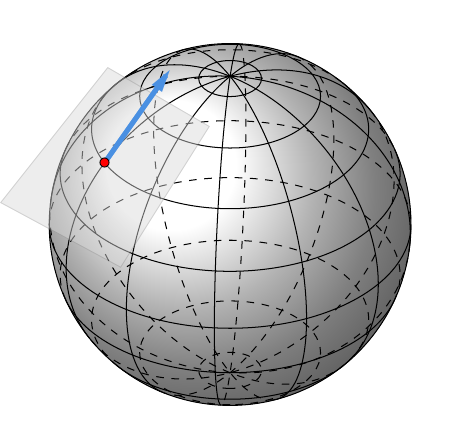
\includegraphics[width=0.3\textwidth]{img/stiefel.png}
%    \caption{
%        Uma Variedade Stiefel no espaço Euclidiano, que quando $b = 1$ essa superfície será uma esfera, e um dos possíveis vetores que está contido no conjunto dessa variedade (tangente à esfera).
%    }
%    \label{fig:stiefel}
%\end{figure}

%\citeonline{Edelman1999} definem o gradiente em um ponto $Y$, com a restrição $Y^T Y = I$, de uma função $\mathcal{J}$ definida em uma Variedade Stiefel no espaço euclidiano como:

%\begin{equation}
%\label{eq:stiefeldiff}
%    \begin{array}{lclcl}
%        {\tilde \nabla}_Y \mathcal{J} & = & \nabla_Y \mathcal{J} - Y (\nabla_Y \mathcal{J})^T Y
%    \end{array}
%\end{equation}

%onde $\nabla_Y \mathcal{J}$ é o gradiente da função $\mathcal{J}$ para todos os elementos da matriz $Y$.

%Dada a equação~\ref{eq:stiefeldiff}, \citeonline{Yoo2010} propõem os seguintes cálculos dos gradientes em Variedades Stiefel para $\mathcal{F}_2$, com $U$ no conjunto $\{ U^T U = I \}$, e com $V$ no conjunto $\{ V^T V = I \}$:

%\[
%    \begin{array}{lclclclcl}
%        {\tilde \nabla_U} \mathcal{F}_2 & = & \nabla_U \mathcal{F}_2 - U (\nabla_U \mathcal{F}_2)^T U & = & U S V^T X^T U - X V S^T \\
%        {\tilde \nabla_V} \mathcal{F}_2 & = & \nabla_V \mathcal{F}_2 - V (\nabla_V \mathcal{F}_2)^T V & = & V S^T U^T X V - X^T U S
%    \end{array}
%\]

%Restando apenas o cálculo do gradiente para $S$, que como não há restrições, será igual à atualização do algoritmo para solução do BVD:

%\[
%    \begin{array}{lclcl}
%        {\tilde \nabla_S} \mathcal{F}_2 & = & \nabla_S \mathcal{F}_2 & = & U^T U S V^T V - U^T X V
%    \end{array}
%\]

Assim,~\citeonline{Yoo2010} faz o uso da estratégia da equação~\ref{eq:onmtf:updateTheta} e da teoria de derivação na superfície com restrições (Variedade Stiefel), para propor uma solução para o problema~\ref{def:onmtf:problem} (\textit{ONMTF}) alternativa às atualizações das equações~\ref{eq:onmtf:updateU},~\ref{eq:onmtf:updateV} e~\ref{eq:onmtf:updateS}, através da atualização multiplicativa.
Essas atualizações são apresentadas no algoritmo~\ref{algo:onmtf2}, considere $t$ o contador de iterações, $U^{(t)}$, $S^{(t)}$ e $V^{(t)}$, as matrizes $U$, $S$ e $V$, na iteração $t$, respectivamente, $\mathcal{U}(0, 1) \in~]0, 1]$ uma função que gera valores de uma distribuição uniforme, $\diag( \cdot )$ uma função que extrai a diagonal principal de uma matriz e a transforma em um vetor, e $\mathbf{1}$ um vetor de uns com dimensão que torne a multiplicação possível.

Considerando a preservação da ortonormalidade, o algoritmo~\ref{algo:onmtf2} é capaz de preservar melhor a ortonormalidade em relação ao algoritmo~\ref{algo:onmtf}.
Para tal afirmação,~\citeonline{Yoo2010} realizou um experimento que consistiu em medir as restrições de ortonormalidade em $U$ e $V$, através dos erros $\norm{U^T U - I}$ e $\norm{V^T V - I}$, respectivamente, durante cada iteração do algoritmo proposto, comparando-o com o algoritmo proposto por~\citeonline{Ding06}.

\begin{algorithm}
\caption{Algoritmo baseado em atualização multiplicativa e na teoria de de derivação na superfície com restrições (Variedade Stiefel) para solução do \textit{ONMTF}}
\label{algo:onmtf2}
\begin{algorithmic}[1]
\Function{ONMTF}{$X$, $k$, $l$, $t_{max}$}
\State \textbf{Inicialize:} $U^{(0)} \gets \mathcal{U}(0, 1), V^{(0)} \gets \mathcal{U}(0, 1), S^{(0)} \gets \mathcal{U}(0, 1)$ e $t \gets 0$.
\While{(não convergiu) e ($t \leq t_{max}$)} %\Comment{We have the answer if r is 0}
\State
\begin{equation}
U^{(t+1)} \gets U^{(t)} \odot \frac{ X V^{(t)} S^{(t)^T} }{ U^{(t)} S^{(t)} V^{(t)^T} X^T U^{(t)} } \nonumber
\end{equation}
\State
\begin{equation}
V^{(t+1)} \gets V^{(t)} \odot \frac{ X^T U^{(t+1)} S^{(t)} }{ V^{(t)} S^{(t)^T} U^{(t+1)^T} X V^{(t)} } \nonumber
\end{equation}
\State
\begin{equation}
S^{(t+1)} \gets S^{(t)} \odot \frac{ U^{(t+1)^T} X V^{(t+1)} }{ U^{(t+1)^T} U^{(t+1)} S^{(t)} V^{(t+1)^T} V^{(t+1)} } \nonumber
\end{equation}
\State $t \gets t + 1$
\EndWhile\label{euclidendwhile}
\State
$$U^{(t)} \gets U^{(t)} \diag(S^{(t)} \diag(\mathbf{1}^T V^{(t)}) \mathbf{1})$$
\State
$$V^{(t)} \gets V^{(t)} \diag(\mathbf{1}^T \diag(\mathbf{1}^T U^{(t)}) S^{(t)})$$
\State \textbf{return} $U^{(t)}, S^{(t)}, V^{(t)}$
\EndFunction
\end{algorithmic}
\end{algorithm}

Ainda,~\citeonline{Yoo2010} propõem uma normalização baseada numa interpretação probabilística da fatoração de $X$ em $USV^T$, para então realizar o particionamento de linhas e colunas, como apresentado no algoritmo~\ref{algo:onmtf2} (linhas $9$ e $10$).
Note que o particionamento de linhas e colunas é realizado como nos outros algoritmos já apresentados, e a mesma condição de convergência aplicada no algoritmo~\ref{algo:bvd} e~\ref{algo:onmtf} pode ser aplicada nesse caso.

Calculando a complexidade de tempo, seguindo as mesmas restrições apresentadas anteriormente para os outros algoritmos, é possível verificar que o algoritmo~\ref{algo:onmtf2}, proposto por~\citeonline{Yoo2010} para solução do problema~\ref{def:onmtf:problem} (\textit{ONMTF}), é equivalente à complexidade apresentada para o algoritmo~\ref{algo:bvd}.

\section{Fatoração Tripla Rápida de Matrizes Não-negativas}
\label{sec:FNMTF}

O problema de Fatoração Tripla Rápida de Matrizes Não-negativas (\textit{Fast Non-negative Matrix Tri Factorization} - FNMTF), formalizado no problema~\ref{def:fnmtf:problem}, foi proposto por~\citeonline{Wang2011} com os seguintes argumentos contra o uso prático dos problemas até então propostos para encontrar cogrupos: eles exigem soluções algorítmicas iterativas, com intensas multiplicações de matrizes em cada passo do algoritmo; eles propõem encontrar coagrupamentos flexíveis (com restrições relaxadas), o que implica em encontrar inúmeras soluções para a tarefa de coagrupamento.

\begin{problem}[Problema de fatoração tripla rápida de matrizes não-negativas]
\label{def:fnmtf:problem}
\begin{equation}
    \begin{array}{lclcl}
        \displaystyle \mathcal{F}_7(U, S, V) & = & \displaystyle \min_{U, S, V} & \norm{X - USV^T}^{2}_{F} \\
                                             &   & \text{suj. a}                & U \in \Psi^{n \times k}, \\
                                             &   &                              & V \in \Psi^{m \times l}, \\
                                             &   &                              & \sum_{p=1}^{k} u_{ip} = 1, \forall i, \\
                                             &   &                              & \sum_{q=1}^{l} v_{jq} = 1, \forall j
    \end{array} \nonumber
\end{equation}
em que $S \in \mathbb{R}^{k \times l}_{+}$e $\Psi = \{0, 1\}$ e $\norm{\cdot}_F$ denota a norma de Frobenius.
\end{problem}

\citeonline{Wang2011} denominam $U$ como uma matriz indicadora dos grupos de linhas, $V$ como uma matriz indicadora dos grupos de colunas, e $S$ como uma matriz que contém os fatores que relacionam um grupo de linhas aos grupos de colunas, e um grupo de colunas aos grupos de linhas.
Note que nesse caso não é necessário uma etapa de pós-processamento para particionamento como nos outros algoritmos apresentados.

Ainda, as restrições $\sum_{p=1}^{k} u_{ip} = 1$ e $\sum_{q=1}^{l} v_{jq} = 1$ indicam que uma linha e uma coluna, respectivamente, têm que pertencer à algum grupo.
Então, apesar dessas restrições serem semelhantes à ortonormalidade, elas não são, pois não resolvem o caso em que há uma possibilidade de haver grupos vazios, ou seja, sem nenhum elemento pertencente a este grupo, enquanto a restrição de ortonormalidade, garante que não haverá grupos vazios, seja este grupo de linhas ou de colunas.

Como $U$ e $V$ neste caso têm as restrições descritas, e são capazes de fornecer o particionamento de linhas e colunas, respectivamente, de forma direta, a capacidade de compactação nesse caso é semelhante ao algoritmo \textit{k-means}, brevemente descrito no capítulo~\ref{ch:conceitos}.
Porém, como a fatoração compacta as colunas e as relações entre grupos de linhas e colunas (matriz $S$), a matriz $X$ é compactada em $n + kl + m$ elementos, e, se $n \ll k$ e $m \ll l$, tem-se que $mm \ll n + kl + m$.

Como não há restrições em $S$, com exceção da positividade que é garantida pela positividade de $X$, é possível encontrar uma regra de atualização para $S$, e portanto, minimização de $\mathcal{F}_7$:
\[
    \begin{array}{lclcl}
        \nabla_S \mathcal{F}_7 &     =    & U^T X V - U^T U S V^T V                     & = & 0                             \\
                               & \implies & U^T U S V^T V                               & = & U^T X V                       \\
                               & \implies & (U^T U)^{-1} U^T U S V^T V (V^T V)^{-1} & = & (U^T U)^{-1} U^T X V (V^T V)^{-1}
    \end{array}   \nonumber
\]

\begin{equation}
\label{eq:fnmtf:updateS}
\begin{array}{lclcl}
\therefore & S & = & (U^T U)^{-1} U^T X V (V^T V)^{-1}    \nonumber
\end{array}
\end{equation}

Assim, o problema de minimização se transforma nos subproblemas de atualização de $U$ e $V$.
Uma estratégia semelhante aquela aplicada no clássico algoritmo \textit{k-means} pode ser aplicada.
Primeiramente, fixa-se $S$ e $V$ e resolve-se o problema~\ref{def:fnmtf:problem} para $U$ de forma iterativa, verificando quais dos protótipos de linhas (linhas de $\widetilde{V}$) mais se aproximam das linhas de $X$.
Em seguida, fixa-se $S$ e $U$ para alcançar uma solução iterativa para $V$, através dos protótipos de colunas (colunas de $\widetilde{U}$), assim como mostrado no algoritmo~\ref{algo:fnmtf}.

Note que é possível interpretar a regra de atualização para $S$: $(U^T U)$ é uma matriz que na diagonal contém a contagem do número de linhas em cada grupo de linhas e zeros nas demais posições, $(U^T U)^{-1}$ é o fator que divide a soma dos valores para cada grupo de linhas, e $U^T X$ seleciona e soma as linhas de $X$ para cada grupo de linhas.
A mesma interpretação pode ser feita para $(V^T V)$, $(V^T V)^{-1}$ e $XV$.
O seguinte exemplo mostra uma matriz de dados com $6$ linhas e $3$ colunas, particionada por $3$ grupos de linhas e $2$ grupos de colunas, ilustrando a interpretação da atualização de $S$:
\[
X = \begin{bmatrix}
\horzbar & \mathbf{x}_{1 \cdot} & \horzbar \\
\horzbar & \mathbf{x}_{2 \cdot} & \horzbar \\
\horzbar & \mathbf{x}_{3 \cdot} & \horzbar \\
\horzbar & \mathbf{x}_{4 \cdot} & \horzbar \\
\horzbar & \mathbf{x}_{5 \cdot} & \horzbar \\
\horzbar & \mathbf{x}_{6 \cdot} & \horzbar
\end{bmatrix}
= \begin{bmatrix}
\vertbar             & \vertbar             & \vertbar             \\
\mathbf{x}_{\cdot 1} & \mathbf{x}_{\cdot 2} & \mathbf{x}_{\cdot 3} \\
\vertbar             & \vertbar             & \vertbar
\end{bmatrix}
\]
\[
U = \begin{bmatrix}
1 & 0 & 0 \\
1 & 0 & 0 \\
0 & 1 & 0 \\
0 & 0 & 1 \\
0 & 1 & 0 \\
1 & 0 & 0
\end{bmatrix},
U^T U = \begin{bmatrix}
3 & 0 & 0 \\
0 & 2 & 0 \\
0 & 0 & 1
\end{bmatrix},
V = \begin{bmatrix}
0 & 1 \\
0 & 1 \\
1 & 0
\end{bmatrix},
V^T V = \begin{bmatrix}
1 & 0 \\
0 & 2
\end{bmatrix}
\]
A matriz $U$ do exemplo apresenta um particionamento das $6$ linhas em $3$ grupos, sendo que $3$ linhas pertencem ao primeiro grupo, $2$ linhas ao segundo grupo, e $1$ linha ao terceiro grupo, como mostra a diagonal principal da matriz $U^T U$, a mesma interpretação pode ser feita para $V$ e $V^T V$.
\[
\begin{array}{ll}
(U^T X) V & = \Bigg(\begin{bmatrix}
1 & 1 & 0 & 0 & 0 & 1 \\
0 & 0 & 1 & 0 & 1 & 0 \\
0 & 0 & 0 & 1 & 0 & 0
\end{bmatrix}
\begin{bmatrix}
\horzbar & \mathbf{x}_{1 \cdot} & \horzbar \\
\horzbar & \mathbf{x}_{2 \cdot} & \horzbar \\
\horzbar & \mathbf{x}_{3 \cdot} & \horzbar \\
\horzbar & \mathbf{x}_{4 \cdot} & \horzbar \\
\horzbar & \mathbf{x}_{5 \cdot} & \horzbar \\
\horzbar & \mathbf{x}_{6 \cdot} & \horzbar
\end{bmatrix}\Bigg)
\begin{bmatrix}
0 & 1 \\
0 & 1 \\
1 & 0
\end{bmatrix}
= \begin{bmatrix}
\mathbf{x}_{1 \cdot} + \mathbf{x}_{2 \cdot} + \mathbf{x}_{6 \cdot} \\
\mathbf{x}_{3 \cdot} + \mathbf{x}_{5 \cdot}                        \\
\mathbf{x}_{4 \cdot}
\end{bmatrix}
\begin{bmatrix}
0 & 1 \\
0 & 1 \\
1 & 0
\end{bmatrix} \\
& = \begin{bmatrix}
x_{13} + x_{23} + x_{63} & x_{11} + x_{12} + x_{21} + x_{22} + x_{61} + x_{62} \\
x_{33} + x_{53}          & x_{31} + x_{32} + x_{51} + x_{52}                   \\
x_{43}                   & x_{41} + x_{42}
\end{bmatrix}
\end{array}
\]
A multiplicação em $X$ por $U^T$ pela esquerda, representa a soma da seleção de todas as linhas de $X$ pertencentes à um mesmo grupo de linhas.
O mesmo ocorre quando multiplica-se $V$ pela direita de $X$, porém, representando a soma da seleção das colunas de $X$ pertencentes à um mesmo grupo de colunas.
Sendo assim, a operação $U^T X V$ representa a soma de todos os elementos de $X$ pertencentes à um mesmo grupo de linhas e colunas, ou seja, por exemplo o elemento da linha $1$ e coluna $1$ de $U^T X V$, que foi calculado no exemplo, é simplesmente a soma de todos os elementos de $X$ que pertencem ao primeiro grupo de linhas e ao primeiro grupo de colunas.\tabularnewline
\[
(U^T U)^{-1} = \begin{bmatrix}
\frac{1}{3} & 0           & 0 \\
0           & \frac{1}{2} & 0 \\
0           & 0           & 1
\end{bmatrix},
(V^T V)^{-1} = \begin{bmatrix}
1 & 0           \\
0 & \frac{1}{2}
\end{bmatrix}
\]
\[
S = (U^T U)^{-1} U^T X V (V^T V)^{-1} = \begin{bmatrix}
\frac{x_{13} + x_{23} + x_{63}}{3} & \frac{x_{11} + x_{12} + x_{21} + x_{22} + x_{61} + x_{62}}{3 \times 2} \\
\frac{x_{33} + x_{53}}{2}          & \frac{x_{31} + x_{32} + x_{51} + x_{52}}{2 \times 2}                   \\
x_{43}                             & \frac{x_{41} + x_{42}}{2}
\end{bmatrix}
\]
Com o exemplo mostrado, é possível visualizar a atualização de $S$ de forma mais intuitiva.
Por exemplo, para calcular um elemento $s_{pq}$ de $S$, será simplesmente o cálculo da média de todos elementos em $X$ que pertencem ao grupo de linhas $p$ e ao grupo de colunas $q$.
Dessa forma, também é possível propor uma solução iterativa para $S$.

O algoritmo~\ref{algo:fnmtf} ilustra o processo de minimização para o problema~\ref{def:fnmtf:problem}.
Nesse algoritmo considere os índices $i \in \{1, \dots, n\}$, $j \in \{1, \dots, m\}$, $p, p' \in \{1, \dots, k\}$, e $q, q' \in \{1, \dots, l\}$, o contador de iterações $t$, $U^{(t)}$, $S^{(t)}$ e $V^{(t)}$ como sendo as matrizes $U$, $S$ e $V$ na iteração $t$, respectivamente, $\mathcal{U}(0, 1) \in~]0, 1]$ uma função que gera valores de uma distribuição uniforme, e $\norm{ \cdot }^2$ é a norma frobenius para vetores.
Também, as mesmas condições de convergência usada nos algoritmos anteriores pode ser aplicada nesse caso.

\begin{algorithm}
\caption{Algoritmo iterativo para solução do \textit{FNMTF}}
\label{algo:fnmtf}
\begin{algorithmic}[1]
\Function{FNMTF}{$X$, $k$, $l$, $t_{max}$}
\State \textbf{Inicialize:} $U^{(0)}, V^{(0)} \gets {0,1}~|~\sum_{p=1}^{k} u_{ip} = 1, \sum_{q=1}^{l} v_{jq} = 1, \forall i, j$, $S^{(0)} \gets \mathcal{U}(0, 1)$ e $t \gets 0$.
\While{(não convergiu) e ($t \leq t_{max}$)}
\State
\begin{equation}
\label{eq:fnmtf:updateS}
S^{(t+1)} \gets (U^{(t)^T} U^{(t)})^{-1} U^{(t)^T} X V^{(t)} (V^{(t)^T} V^{(t)})^{-1}   \nonumber
\end{equation}
\State
\[
\widetilde{V} \gets S^{(t+1)} V^{(t)^T}
\]
\State
\begin{equation}
\label{eq:fnmtf:updateF}
(U^{(t+1)})_{ip} \gets \left\{
\begin{array}{ll}
1 & p = \argmin_{p' \in \{1, \dots, k\}} \norm{ \mathbf{x}_{i \cdot} - \widetilde{\mathbf{v}}_{p' \cdot} }^2 \\
0 & \textit{caso contrário}
\end{array}    \nonumber
\right. \forall i, p
\end{equation}
\State
\[
\widetilde{U} \gets U^{(t+1)} S^{(t+1)}
\]
\State
\begin{equation}
\label{eq:fnmtf:updateG}
(V^{(t+1)})_{jq} \gets \left\{
\begin{array}{ll}
1 & q = \argmin_{q' \in \{1, \dots, l\}} \norm{ \mathbf{x}_{\cdot j} - \widetilde{\mathbf{u}}_{\cdot q'} }^2 \\
0 & \textit{caso contrário}
\end{array}      \nonumber
\right. \forall j, q
\end{equation}
\State $t \gets t + 1$
\EndWhile\label{euclidendwhile}
\State \textbf{return} $U^{(t)}, S^{(t)}, V^{(t)}$
\EndFunction
\end{algorithmic}
\end{algorithm}

A análise de complexidade de tempo do algoritmo~\ref{algo:fnmtf} difere das demais apresentadas.
Se for usado um algoritmo iterativo para o cálculo das matrizes inversas, aproveitando o fato que ambas contém elementos diferentes de $0$ na diagonal principal, é possível chegar no seguinte resultado: $\mathcal{O}\Big( t_{max} \big( nl (m + k) + kl (n + m) + nk + ml \big) \Big) \simeq \mathcal{O}\Big( t_{max} \big( n^2k + k^2n + nk \big) \Big)$.
Já é possível perceber que a complexidade do algoritmo é menor que a complexidade dos algoritmos~\ref{algo:bvd},~\ref{algo:onmtf} e~\ref{algo:onmtf2}.
Isso se explica pois a atualização de $U$ e $V$ é feita de forma iterativa.
Ainda, as multiplicações de matrizes para o cálculo dos centróides $\widetilde{U}$ e $\widetilde{V}$, e para atualização de $S$, que podem ser calculadas de forma iterativa, melhorando ainda mais a complexidade de tempo do algoritmo.

% ************************************************************

\section{Considerações finais}

% Sara: não consigo colocar o exemplo do Valdinei, pois eu precisaria de um exemplo real para conseguir explicar com números e esse exemplo só virá no Capítulo 5. Colocar de forma genérica, eu também não consegui. Tentei mas tive a impressão de estar apenas repetindo as formulações dos problemas já apresentadas. Então resolve usar "prosa" mesmo. Um texto equivalente deveria ser feito para o K-means e para o Fuzzy-K-means no final do capítulo 2.

É importante ressaltar, que nenhum dos algoritmos apresentados são capazes de garantir convergência para um mínimo global dos problemas apresentados, então, é possível encontrar diversas soluções em execuções diferentes dos algoritmos, devido à inicialização de forma aleatória.
Essa é uma limitação também presente nos algoritmos de agrupamento clássicos.

Além disso, a fim de melhor motivar a proposta dos novos algoritmos apresentados no capítulo~\ref{ch:proposedalgs}, é interessante compreender os algoritmos \textit{ONMTF} e \textit{FNMTF} em termos de suas capacidades de quantização do espaço dos dados e de geração de informação sobre os dados, e em termos do processo de descoberta de cogrupos.

Do ponto de vista de quantização do espaço dos dados, a quantidade de informação que precisa ser armazenada é dependente da organização da matriz $S$, ou seja, do número de grupos de linhas $k$ e do número de colunas $l$ necessários para explicar a matriz de dados original.
Como será discutido mais à frente neste trabalho, para determinados tipos de organizações de cogrupos, especificamente aqueles em que há sobreposição de colunas nos grupos de colunas, os algoritmos implementados sob essas estratégias exigem uma quantidade de grupos de colunas ($l$) que pode ser maior do que o número de grupos de colunas desejados.
Os algoritmos propostos têm o objetivo de superar essa limitação, permitindo que a quantização do espaço seja mais próxima da desejada em termos de grupos de colunas.

Do ponto de vista de geração de informação sobre os dados, os algoritmos \textit{ONMTF} e \textit{FNMTF} são capazes de fornecer como as linhas da matriz se organizam em grupos e como as colunas da matriz se organizam em grupos.
Transferindo essa informação para um contexto de aplicação, significa dizer que os algoritmos são capazes de explicar como os dados se organizam no espaço (matriz $U$) e, intuitivamente e sob uma forma de organização, como grupos de atributos desses dados (matriz $V$) podem estar associados (por meio da matriz $S$) à essa organização dos dados.
Esse tipo de informação, também presente nos algoritmos propostos, não é explicitamente fornecida por algoritmos de agrupamento como \textit{k-means} e \textit{fuzzy k-means}, discutidos no capítulo~\ref{ch:conceitos}.

Do ponto de vista do processo de descoberta dos cogrupos, os algoritmos \textit{ONMTF} e \textit{FNMTF} são capazes de considerar simultâneamente ambas organizações na resolução do problema de minimização do erro de quantização da matriz original.
Porém, possuem um processo que pode ser caracterizado por um tipo de interdependência entre grupos de linhas, que é na realidade o causador da possibilidade de chegar a uma quantidade de grupos de colunas ($l$) maior do que é realmente necessário para explicar os dados que possuem uma organização de cogrupos com sobreposição de colunas.
Esta é a segunda meta de superação obtida nos algoritmos propostos, que por sua formulação, são capazes de resolver o problema de fatoração das matrizes de maneira independente para cada grupo de linhas.

% Uma observação que pode ser feita, é que as fatorações apresentadas nesta seção, consideram a interdependência entre todas as linhas para construção dos protótipos de colunas, ou seja, um padrão tem que estar presente em todas as linhas para que seja formado um protótipo capaz de reconstruir a matriz original.
% Isso poderia ser diferente caso os protótipos de colunas fossem formados com as linhas de um determinado grupo de linhas.
% Esse comportamento também pode ser feito com os grupos de linhas.

% Esses problemas devem ficar para o final, para dar o link para trabalhos futuros e para limitações deste trabalho
% Finalmente, é preciso salientar que embora os algoritmos ONMTF e FNMTF possuam características interessantes sobre análise de dados, que superam algoritmos clássicos de análise de dados como k-means e fuzzy-k-means (como mostrado nos resultados apresentados no capítulo~\ref{ch:experiments}, esses são computacionalmente mais caros. E, ainda, os algoritmos propostos, embora sejam capazes de superar limitações do ONMTF e FNMTF, se apresentam como algoritmos de um custo ainda mais elevado computacionalmente.

% ************************************************************
% ************************************************************
% ************************************************************

\chapter{Fatoração de matrizes não-negativas para coagrupamento com sobreposição de colunas}
\label{ch:proposedalgs}

Como discutido no capítulo~\ref{ch:fatoracao}, a fatoração de matrizes aplicada ao problema de agrupamento ou coagrupamento pode ser analisada sob, pelo menos, três aspectos: quantização do espaço dos dados; geração de informação sobre os dados; e pelo processo de descoberta de cogrupos.
Também, para cada uma dessas análises, diferentes estratégias apresentam vantagens e desvantagens.

Com o intuito de apresentar uma alternativa às estratégias de fatoração de matrizes não-negativas para coagrupamento presentes na literatura, objetivando superar algumas das dificuldades apresentadas por eles, propõe-se duas novas estratégias que adicionam $k$ matrizes $V$ na fatoração, ao invés de uma única matriz $V$.
Basicamente, cada uma dessas matrizes representará uma organização de cogrupos de colunas independente, de maneira que aumentar-se-á a flexibilidade para o estabelecimento de relações entre cogrupos de linhas e cogrupos de colunas.
As estratégias são:

\begin{itemize}
\item \textit{OvNMTF}: uma estratégia de fatoração tripla de matrizes não-negativas com sobreposição de colunas, baseada na estratégia \textit{BVD};
\item \textit{BinOvNMTF}: uma estratégia de fatoração binária tripla de matrizes não-negativas com sobreposição de colunas, baseada na estratégia \textit{FNMTF}.
\end{itemize}

Sob o ponto de vista de resolução de problemas de coagrupamento, o objetivo dessas estratégias é o mesmo das estratégias já apresentadas neste texto, qual seja, encontrar grupos de linhas e colunas de forma simultânea.
Entretanto, visto que se tem a liberdade de organizar um conjunto de matrizes $V$, que abstrai grupos e colunas, para ser associado a cada grupo de linhas, que abstrai os grupos de linhas, é possível que grupos de colunas diferentes sejam formados, a depender do grupo de linhas sendo considerado.
Isso significa que problemas em que há sobreposição de colunas na formação de cogrupos, poderão ser adequadamente tratados pelas estratégias propostas.

Formalmente, considere uma matriz de dados $X \in \mathbb{R}^{n \times m}$ contendo números reais positivos com $n$ linhas e $m$ colunas, formada por um conjunto de vetores de linhas $\mathcal{N} = \{ \mathbf{x}_{1 \cdot}, \dots, \mathbf{x}_{n \cdot} \}$ e um conjunto de vetores de colunas $\mathcal{M} = \{\mathbf{x}_{\cdot 1}, \dots, \mathbf{x}_{\cdot m} \}$, e as relações existentes entre cada linha $\mathbf{x}_{i \cdot}$ e cada coluna $\mathbf{x}_{\cdot j}$ são representadas por $x_{ij}$ considerando os índices $i \in \{1, \dots, n\}$ e $j \in \{1, \dots, m\}$.
Cada valor em $x_{ij}$ representa, então, a relação existente entre pares de elementos em algum contexto de interesse.
O objetivo da tarefa de coagrupamento sob a estratégia de coagrupamento é encontrar $k$ partições de $\mathcal{N}$, denotadas pelos subconjuntos ordenados $\mathcal{K}_p \subseteq \mathcal{N}$, $k \times l$ partições para $\mathcal{M}$ em cada $\mathcal{K}_p$, denotadas pelos subconjuntos ordenados $\mathcal{L}_{pq} \subseteq \mathcal{M}$, considerando os índices $p \in \{ 1, \dots, k\}$ e $q \in \{1, \dots, l\}$.
Então, os conjuntos $\{\mathcal{K}_1, \dots, \mathcal{K}_k\}$ e $\{\mathcal{L}_{11}, \dots, \mathcal{L}_{1l}, \dots, \mathcal{L}_{k1}, \dots \mathcal{L}_{kl}\}$ são os cogrupos de linhas e colunas, respectivamente.

Observe na figura~\ref{fig:ovnmtfApplication} uma representação gráfica da estrutura de cogrupos com sobreposição de colunas, contextualizado em uma aplicação de análise de textos.
Note que, na realidade, trata-se de busca por uma solução adequada para um problema com sobreposição, ou seja, sobreposição de colunas ou de linhas, já que a sobreposição de linhas é justamente o problema transposto.

A figura~\ref{fig:ovnmtfApplication} mostra dois grupos de documentos, dos assuntos games e tecnologia, com três documentos em cada.
Ainda, este exemplo contém $6$ grupos de palavras, divididos igualmente entre os grupos de documentos.
Então, pode-se dizer que os grupos de palavras entitulados ``campeonatos'', ``consoles'' e ``games online'' caracterizam o grupo de documentos sobre games, assim como os grupos de palavras entitulados ``competições'', ``eletrônicos'' e ``software'' caracterizam o grupo de documentos sobre tecnogia.
Note que há sobreposição entre os primeiros três grupos de palavras do grupo de documentos com os três primeiros grupos de palavras do grupo de documentos de tecnologia.
Também, é possível observar que apesar das palavras serem as mesmas para todos os documentos, como há independência entre os grupos de palavras para cada grupo de documentos, as palavras caracterizaram grupos de palavras diferentes, como no exemplo, os grupos de palavras entitulados como ``games online'' e ``software''.

% Lucas: Fico pensando, depois de ter feito essa figura, se os nossos algoritmos resolvem o problema de `polysemous word`, que o \cite{Yoo2010} fala no final do paper (seção 4.3): uma palavra pode significar uma coisa em um contexto e no outro contexto, ela significa outra coisa

\begin{figure}[H]
\centering
\caption{Representação gráfica do problema de coagruamento com sobreposição de colunas e contextualização do domínio de documentos (notícias)}
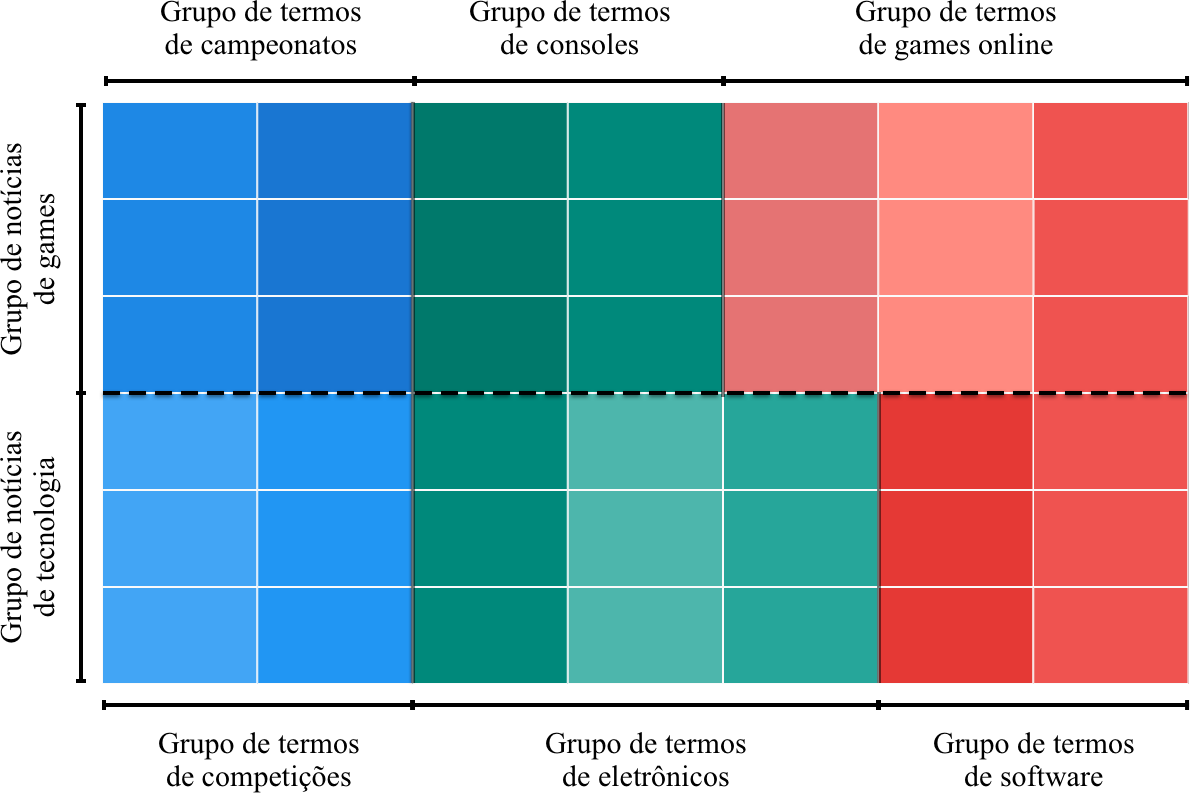
\includegraphics[width=0.5\textwidth]{img/ovnmtfNewsApplication.png}
\label{fig:ovnmtfApplication}
\source{Lucas Fernandes Brunialti, 2016}
\end{figure}

Da mesma maneira que foi ilustrado no capítulo~\ref{ch:fatoracao}, que é possível derivar interpretações intuitivas da análise das combinações de matrizes geradas na fatoração produzida pelos algoritmos lá discutidos.
Para os algoritmos discutidos no presente capítulo, interpretações análogas podem ser feitas, porém, consirando a existências das várias matrizes $V$.
Assumindo novamente que uma matriz de entrada representa a relação ``documento por palavras'' (linhas por colunas), cada coluna das $k$ matrizes $U I_{(p)} S, \forall p \in \{1, \dots, k\}$, captura a ideia de uma base para representação de grupos de palavras, descritos nas matrizes $V_{(p)}$; e cada linha em $\sum_{p=1}^k I_{(p)} S V_{(p)}^T$, captura a ideia de uma base de representação de grupos de documentos.
A representação gráfica para o resultado de uma fatoração de matrizes que permite esse raciocínio é apresentada na figura~\ref{fig:factorizationXUSV1tok}.

\begin{figure}[H]
\centering
\caption{
Fatoração da matriz original de dados $X$ em cinco outras matrizes: $U$, $S$, $V_1$, $V_2$ e $V_3$}
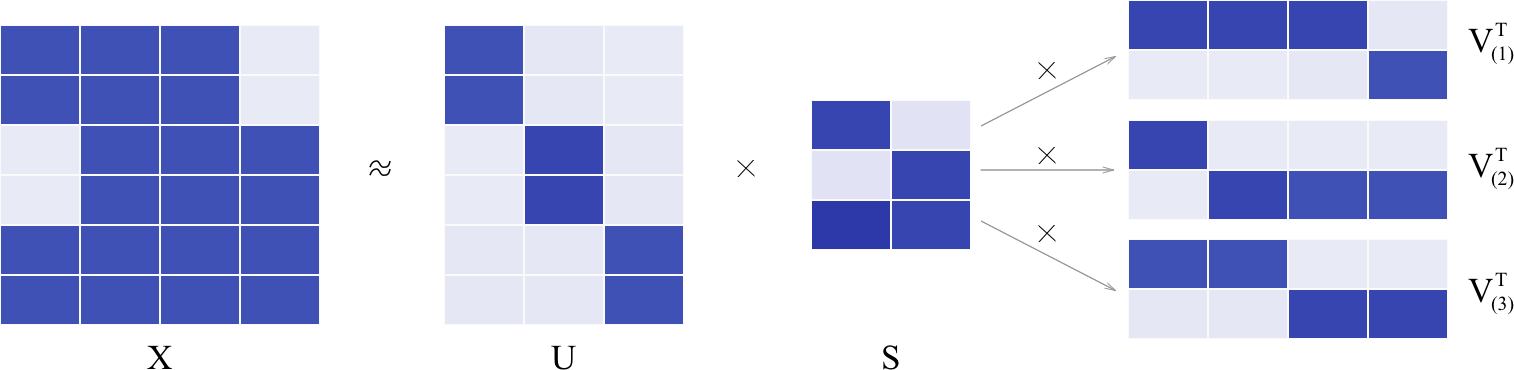
\includegraphics[width=0.8\textwidth]{img/factorizationXUSV1tok.png}
\label{fig:factorizationXUSV1tok}
\source{Lucas Fernandes Brunialti, 2016}
\end{figure}

Todo o universo de interpretações delineado para os algoritmos da literatura podem ser estendidos para esse novo contexto de problema de agrupamento.
No entanto, agora existem três matrizes para determinar os grupos de palavras, cada uma delas responsável por determinar os grupos de palavras para cada grupo de documentos.
Na figura~\ref{fig:factorizationXUSV1tok} considere que uma célula com cor escura representa a existência de uma relação entre linha e coluna, e uma célula com cor clara representa a inexistência de uma relação entre linha e coluna, e que essas relações são estabelecidas adequadamente em cada contexto de aplicação.
Tem-se então, um conjunto de seis documentos e quatro palavras.
A matriz $U$ pode ser interpretada como descrito anteriormente, uma matriz ``documentos por grupos de documentos'', com seis documentos agrupados em três grupos ($k = 3$): os dois primeiros documentos no primeiro grupo, os dois próximos no segundo grupo e os dois últimos no terceiro grupo.
Já as matrizes $V_{(p)}^T$ têm uma interpretação levemente diferente, ainda podem ser interpretadas como matrizes de ``grupos de palavras por palavras'', sendo dois grupos de palavras ($l = 2$), porém, a matriz $V_{(1)}^T$, por exemplo, contém os grupos de palavras para o primeiro grupo de documentos apenas (composto pelas linhas $1$ e $2$ de $X$), no primeiro grupo de palavras estão as colunas $1$, $2$ e $3$, e no segundo, a coluna $4$.
O mesmo raciocínio pode ser utilizado para as matrizes $V_{(2)}^T$ e $V_{(3)}^T$.
Por fim, para a matriz $S$ pode ser realizada a mesma interpretação, representando uma relação entre grupos de documentos e grupos de palavras, com a ressalva de que irão existir $k \times l$ grupos de palavras, ou seja, a linha $p$ da matriz $S$ irá representar a relação entre o $p$-ésimo grupo de documentos e os grupos de palavras encontrados em $V_{(p)}^T$.

O restante deste capítulo é destinado a apresentar a formulação dos problemas para cada uma das estratégias, incluindo a apresentação de uma derivação teórica para um algoritmo que implementa o processo de resolução para os problemas.
Finalmente, as considerações finais apresentam uma discussão sobre o diferencial dessas estratégias no que diz respeito aos três aspectos citados no início do capítulo.

\section{Fatoração Tripla de Matrizes Não-negativas com Sobreposição}

Baseado no problema~\ref{def:bvd:problem}~\cite{Long2005}, o problema~\ref{def:ovnmtf:problem} é apresentado neste trabalho, e recebe aqui o nome de Fatoração Tripla de Matrizes Não-negativas Sobrepostas (Overlapped Non-negative Matrix Tri-factorization - \textit{OvNMTF}).

\begin{problem}[Problema de fatoração tripla de matrizes não-negativas sobrepostas]
\label{def:ovnmtf:problem}
\begin{equation}
    \begin{array}{lclc}
        \displaystyle \mathcal{F}_6(U, S, V_{(1)}, \dots, V_{(k)}) & = & \displaystyle \min_{U, S, V_{(1)}, \dots, V_{(k)}} & \norm{X - U\sum_{p=1}^{k}I_{(p)}SV_{(p)}^T}^{2}_{F} \\
                                                                   &   & \text{suj. a}                & U \geq 0, S \geq 0, \\
                                                                   &   &                              & V_{(p)} \geq 0, \quad \forall p
    \end{array} \nonumber
\end{equation}
em que $U \in \mathbb{R}^{n \times k}_{+}$, $S \in \mathbb{R}^{k \times l}_{+}$, $V_{(p)} \in \mathbb{R}^{m \times l}_{+}$, $p \in \{1, \dots, k\}$ é o índice para o conjunto de matrizes $\{ V_{(1)}, \dots, V_{(k)} \}$, $I_{(p)} \in \{0,1\}^{k \times k}$ é uma matriz seletora com zeros em todos elementos exceto o elemento $i_{(p)_{pp}}$ que é igual à $1$, e $\norm{\cdot}_F$ denota a norma de Frobenius.
\end{problem}

Na formulação, o papel das matrizes $I_{(p)}$ seletoras é, justamente, organizar a base de grupos de linhas, de forma que cada um deles seja otimizado de acordo com uma das matrizes $V_{(p)}$.

É possível perceber que, neste caso, diferente dos apresentados no capítulo~\ref{ch:fatoracao}, têm menor capacidade de compactação, porém, com maior nível de detalhamento.
Isso se explica, pois a partir dos $nm$ elementos da matriz de dados, são gerados $nk + kl + klm$ para representá-los, diferente.

Desde que o problema~\ref{def:ovnmtf:problem} é semelhante ao problema~\ref{def:onmtf:problem}, é esperado que ele possa também ser resolvido por meio de regras de atualização multiplicativas.
Assim, a derivação das regras é aqui apresentada por meio de um abordagem baseada no cálculo do gradiente.
Contudo, para o cálculo do gradiente de $\mathcal{F}_6$ a estratégia usada aqui é a apresentada em~\citeonline{Yoo2010}, de forma que $\nabla \mathcal{F}_6 = [\nabla \mathcal{F}_6]^+ - [\nabla \mathcal{F}_6]^-$.\blfootnote{Considere as seguintes igualdades para o cálculo dos gradientes, já definidas no capítulo~\ref{ch:conceitos}, sendo $A, B, C$ e $D$ matrizes de quaisquers dimensões adequadas para a realização das multiplicações:
\begin{equation}
\label{eq:diff:AQB}
\begin{array}{lcl}
\nabla_A tr( BAC )     & = & A^T B^T \\
\nabla_{A^T} tr( BAC ) & = & C B \\
\end{array}
\end{equation}

\begin{equation}
\label{eq:diff:AQBQtC}
\begin{array}{lcl}
\nabla_A tr( BACA^TD )     & = & B^TD^TAC^T + DBAC \\
\nabla_{A^T} tr( C^TA^TDAC ) & = & CA^TDB + C^TA^TB^TD^T
\end{array}
\end{equation}
}

Expandindo $\mathcal{F}_6$, com base nas propriedade de traço de matrizes definidas no capítulo~\ref{ch:conceitos}, para tornar o cálculo do gradiente mais simples, é possível obter:
\[
    \begin{array}{lcl}
        \displaystyle \mathcal{F}_6 & = & tr\big[ (X - U\sum_{p=1}^{k}I_{(p)}SV_{(p)}^T)^T (X - U\sum_{p=1}^{k}I_{(p)}SV_{(p)}^T) \big] \\
                                    & = & tr(X^TX) - 2 tr( X^T U \sum_{p=1}^{k} I_{(p)} S V_{(p)}^T ) + tr( \sum_{p=1}^{k} V_{(p)} S^T I_{(p)} U^T U \sum_{p'=1}^k I_{(p')} S V_{(p')}^T )
    \end{array}
\]

Note que a matriz seletora tem a seguinte propriedade: $I_{(p)}^T = I_{(p)}$.

Para o cálculo de $\nabla_U \mathcal{F}_6$, considere as partes positiva e negativa desse gradiente, $[\nabla_U \mathcal{F}_6]^+$ e $[\nabla_U \mathcal{F}_6]^-$, respectivamente.
Usando a igualdade da equação~\ref{eq:diff:AQB}, com $B = X^T$, $C = \sum_{p=1}^{k}I_{(p)}SV_{(p)}^T$ e $A = U$, é possível obter $[\nabla_U \mathcal{F}_6]^-$, como segue.
\[
    \begin{array}{lcl}
        [\nabla_U \mathcal{F}_6]^- & = & - 2 \nabla_U \Big( tr\big[ X^T U \sum_{p=1}^{k}I_{(p)}SV_{(p)}^T \big] \Big) \\
                                   & = & - 2 X \sum_{p=1}^{k} V_{(p)} S^T I_{(p)}
    \end{array}
\]

Para o cálculo de $[\nabla_U \mathcal{F}_6]^+$, é utilizado a igualdade da equação~\ref{eq:diff:AQBQtC}, com $B = \sum_{p=1}^{k} V_{(p)} S^T I_{(p)}$, $C = I$, $A = U^T$ e $D = \sum_{p'=1}^{k}I_{(p')}SV_{(p')}^T$.
Então tem-se
\[
    \begin{array}{lcl}
        [\nabla_U \mathcal{F}_6]^+ & = & \nabla_U \Big( tr(X^TX) + tr\big[ \sum_{p=1}^{k} V_{(p)} S^T I_{(p)} U^T U \sum_{p'=1}^k I_{(p')} S V_{(p')}^T \big] \Big) \\
                                   & = & U \sum_{p'=1}^k I_{(p')} S V_{(p')}^T \sum_{p=1}^{k} V_{(p)} S^T I_{(p)} \\
                                   &   & + ~ U \sum_{p=1}^k I_{(p)} S V_{(p)}^T \sum_{p'=1}^{k} V_{(p')} S^T I_{(p')} \\
                                   & = & 2 U \sum_{p=1}^k \sum_{p'=1}^{k} I_{(p)} S V_{(p)}^T V_{(p')} S^T I_{(p')}
    \end{array}
\]

De forma similar, para o cálculo de $\nabla_S \mathcal{F}_6$, considere as partes positiva e negativa, $[\nabla_S \mathcal{F}_6]^+$ e $[\nabla_S \mathcal{F}_6]^-$, respectivamente.
Usando a igualdade da equação~\ref{eq:diff:AQB} para todas as partes da soma de $p \in \{1, \dots, k\}$, com $B = X^T U I_{(p)}$, $A = S$, e $C = V_{(p)}^T$, é possível obter $[\nabla_S \mathcal{F}_6]^-$, como segue:
\[
    \begin{array}{lcl}
        [\nabla_S \mathcal{F}_6]^- & = & - 2 \nabla_S \Big( tr\big[ X^T U I_{(1)}SV_{(1)}^T \big] + \dots + tr\big[ X^T U I_{(k)}SV_{(k)}^T \big] \Big) \\
                                   & = & - 2 \Big( I_{(1)} U^T X V_{(1)} + \dots + I_{(k)} U^T X V_{(k)} \Big) \\
                                   & = & - 2 \sum_{p=1}^{k} I_{(p)} U^T X V_{(p)}
    \end{array}
\]

Para o cálculo de $[\nabla_S \mathcal{F}_6]^+$, é utilizado a igualdade da equação~\ref{eq:diff:AQBQtC} para todas as partes da soma de $p, p' \in \{1, \dots, k\}$, com $B = V_{(p)}$, $A = S^T$, $C = I_{(p)} U^T U I_{(p')}$ e $D = V_{(p')}^T$.
Então tem-se
\[
    \begin{array}{lcl}
        [\nabla_S \mathcal{F}_6]^+ & = & \nabla_S \Big( tr(X^TX) + tr\big[ V_{(1)} S^T I_{(1)} U^T U I_{(1)} S V_{(1)}^T \big] + \dots + tr\big[ V_{(1)} S^T I_{(1)} U^T U I_{(k)} S V_{(k)}^T \big]  \\
                                   &   & + \dots + tr\big[ V_{(k)} S^T I_{(k)} U^T U I_{(1)} S V_{(1)}^T \big] + \dots + tr\big[ V_{(k)} S^T I_{(k)} U^T U I_{(k)} S V_{(k)}^T \big] \Big) \\
                                   & = & \big( I_{(1)} U^T U I_{(1)} S V_{(1)}^T V_{(1)} + I_{(1)} U^T U I_{(1)} S V_{(1)}^T V_{(1)} \big) \\
                                   &   & + \dots + \big( I_{(1)} U^T U I_{(k)} S V_{(k)}^T V_{(1)} + I_{(k)} U^T U I_{(1)} S V_{(1)}^T V_{(k)} \big) \\
                                   &   & + \dots + \big( I_{(k)} U^T U I_{(1)} S V_{(1)}^T V_{(k)} + I_{(1)} U^T U I_{(k)} S V_{(k)}^T V_{(1)} \big) \\
                                   &   & + \dots + \big( I_{(k)} U^T U I_{(k)} S V_{(k)}^T V_{(k)} + I_{(k)} U^T U I_{(k)} S V_{(k)}^T V_{(k)} \big) \\
                                   & = & 2 \sum_{p=1}^{k} \sum_{p'=1}^{k} I_{(p)} U^T U I_{(p')} S V_{(p')}^T V_{(p)}
    \end{array}
\]


Finalmente, para o cálculo de $\nabla_{V_{(p)}} \mathcal{F}_6$, considere as partes positiva e negativa, $[\nabla_{V_{(p)}} \mathcal{F}_6]^+$ e $[\nabla_{V_{(p)}} \mathcal{F}_6]^-$, respectivamente. Usando a igualdade da equação~\ref{eq:diff:AQB}, com $B = X^T U I_{(p)} S$, $A = V^{T}_{(p)}$, e $C = I$, $\forall p$, é possível obter $[\nabla_{V_{(p)}} \mathcal{F}_6]^-$, da seguinte forma:
\[
    \begin{array}{lcl}
        [\nabla_{V_{(p)}} \mathcal{F}_6]^- & = & - 2 \nabla_{V_{(p)}} \Big( tr\big[ X^T U I_{(1)}SV_{(1)}^T \big] + \dots + tr\big[ X^T U I_{(k)}SV_{(k)}^T \big] \Big) \\
                                           & = & - 2 X^T U I_{(p)} S
    \end{array}
\]

Na derivação para $[\nabla_{V_{(p)}} \mathcal{F}_6]^+$ nota-se que há dois casos diferentes para a derivação. O caso em que $p = p'$ e o caso em que $p \neq p'$. Para o caso em que $p = p'$, é utilizada a igualdade da equação~\ref{eq:diff:AQBQtC}, com $B = I$, $A = V_{(p)}$, $C = S^T I_{(p)} U^T U I_{(p)} S$ e $D = I$, $\forall p$, de forma que
\[
    \begin{array}{lcl}
        [\nabla_{V_{(p)}} \mathcal{F}_6]^{+}_{p=p'} & = & \nabla_{V_{(p)}} \Big( tr\big[ V_{(1)} S^T I_{(1)} U^T U I_{(1)} S V_{(1)}^T \big] + \dots + tr\big[ V_{(k)} S^T I_{(k)} U^T U I_{(k)} S V_{(k)}^T \big] \Big) \\
                                                    & = & \nabla_{V_{(p)}} \Big( tr\big[ V_{(p)} S^T I_{(p)} U^T U I_{(p)} S V_{(p)}^T \big] \Big)  \\
                                                    & = & 2 V_{(p)} S^T I_{(p)} U^T U I_{(p)} S
    \end{array}
\]

Para o caso em que $p \neq p'$, é usada a igualdade da equação~\ref{eq:diff:AQB} em duas outras situações, aquela em que $V_{(p)}$ esta localizado à esquerda, então, $A = V_{(p)}$, $B = I$ e $C = S^T I_{(p)} U^T U I_{(p')}$; e aquela em que $V_{(p)}$ esta localizado à direita, então, $A = V_{(p)}^T$, $B = V_{(p')} S^T I_{(p')} U^T U I_{(p)} S$, $C = I$, $\forall p, p'$. Assim,
\[
    \begin{array}{lcl}
        [\nabla_{V_{(p)}} \mathcal{F}_6]^{+}_{p \neq p'} & = & \nabla_{V_{(p)}} \Big( tr\big[ V_{(1)} S^T I_{(1)} U^T U I_{(2)} S V_{(2)}^T \big] + \dots + tr\big[ V_{(1)} S^T I_{(1)} U^T U I_{(k)} S V_{(k)}^T \big] \\
                                   &   & + \dots + tr\big[ V_{(k)} S^T I_{(k)} U^T U I_{(1)} S V_{(1)}^T \big] + \dots + tr\big[ V_{(k)} S^T I_{(k)} U^T U I_{(k-1)} S V_{(k-1)}^T \big] \Big) \\
                                   & = & \sum_{p' \neq p} \bigg[ \nabla_{V_{(p)}} \Big( tr\big[ V_{(p)} S^T I_{(p)} U^T U I_{(p')} S V_{(p')}^T \big] \Big) \\
                                   &   & + ~ \nabla_{V_{(p)}} \Big( tr\big[ V_{(p')} S^T I_{(p')} U^T U I_{(p)} S V_{(p)}^T \big] \Big) \bigg] \\
                                   & = & \sum_{p' \neq p} 2 \big( V_{(p')} S^T I_{(p')} U^T U I_{(p)} S \big)
    \end{array}
\]

Então, é possível calcular $[\nabla_{V_{(p)}} \mathcal{F}_6]^{+}$, $\forall p$, fazendo:
\[
    \begin{array}{lcl}
        [\nabla_{V_{(p)}} \mathcal{F}_6]^{+} & = & [\nabla_{V_{(p)}} \mathcal{F}_6]^{+}_{p = p'} + [\nabla_{V_{(p)}} \mathcal{F}_6]^{+}_{p \neq p'} \\
                                             & = & 2 \big( V_{(p)} S^T I_{(p)} U^T U I_{(p)} S + \sum_{p' \neq p} V_{(p')} S^T I_{(p')} U^T U I_{(p)} S \big) \\
                                             & = & 2 \big( \sum_{p'=1}^{k} V_{(p')} S^T I_{(p')} U^T U I_{(p)} S \big)
    \end{array}
\]

O resultado final dos gradientes para $U, S, V_{(p)}, \forall p \in \{1, \dots, k\}$ são apresentados nas equações~\ref{eq:ovnmtf:gradU},~\ref{eq:ovnmtf:gradS} e~\ref{eq:ovnmtf:gradV}, respectivamente.
\begin{equation}
\label{eq:ovnmtf:gradU}
    \begin{array}{lcl}
        \nabla_U \mathcal{F}_6 & = & 2 \big( - X \sum_{p=1}^{k} V_{(p)} S^T I_{(p)} + U \sum_{p=1}^k \sum_{p'=1}^{k} I_{(p)} S V_{(p)}^T V_{(p')} S^T I_{(p')} \big)
    \end{array}
\end{equation}
\begin{equation}
\label{eq:ovnmtf:gradS}
    \begin{array}{lcl}
        \nabla_S \mathcal{F}_6 & = & 2 \big( - \sum_{p=1}^{k} I_{(p)} U^T X V_{(p)} + \sum_{p=1}^{k} \sum_{p'=1}^{k} I_{(p)} U^T U I_{(p')} S V_{(p')}^T V_{(p)} \big)
    \end{array}
\end{equation}
\begin{equation}
\label{eq:ovnmtf:gradV}
    \begin{array}{lcl}
        \nabla_{V_{(p)}} \mathcal{F}_6 & = & 2 \big( -X^T U I_{(p)} S + \sum_{p'=1}^{k} V_{(p')} S^T I_{(p')} U^T U I_{(p)} S \big)
    \end{array}
\end{equation}

Sendo assim, as regras de atualização para as matrizes $U, V_{(p)}, S, \forall p \in \{1, \dots, k\}$, são mostradas nas equações~\ref{eq:ovnmtf:updateU},~\ref{eq:ovnmtf:updateV} e~\ref{eq:ovnmtf:updateS}, apresentadas no algoritmo~\ref{algo:ovnmtf}, o qual implementa o processo de minimização para o problema~\ref{def:ovnmtf:problem}.
Nesse algoritmo, $t$ é o contador de iterações, $U^{(t)}$, $S^{(t)}$ e $V_{(p)}^{(t)}$ são as matrizes $U$, $S$ e $V_{(p)}$, na iteração $t$, respectivamente, e $\mathcal{U}(0, 1) \in~]0, 1]$ uma função que gera valores de uma distribuição uniforme.

% TODO: condições de convergência não foram provadas, mas podemos dar algum insight sobre isso?

\begin{algorithm}[H]
\caption{Algoritmo baseado em atualização multiplicativa para solução do \textit{OvNMTF}}
\label{algo:ovnmtf}
    \begin{algorithmic}[1]
        \Function{OvNMTF}{$X$, $k$, $l$, $t_{max}$}
            \State \textbf{Inicialize:} $U^{(0)} \gets \mathcal{U}(0,1), S^{(0)} \gets \mathcal{U}(0,1), V_{(p)}^{(0)} \gets \mathcal{U}(0,1), \forall p$ e $t \gets 0$.
            \While{(não convergiu) e ($t \leq t_{max}$)} %\Comment{We have the answer if r is 0}
                \State
                    \begin{equation}
                    \label{eq:ovnmtf:updateU}
                        U^{(t+1)} \gets U^{(t)} \odot \frac{ \sum_{p=1}^{k} X V^{(t)}_{(p)} S^{(t)^T} I_{(p)} }{ \sum_{p=1}^{k} \sum_{p'=1}^k U^{(t)} I_{(p)} S^{(t)} V^{(t)^T}_{(p)} V^{(t)}_{(p')} S^{(t)^T} I_{(p')} }
                    \end{equation}
                \For{$p \leftarrow 1 \text{ até } k$}
                    \State
                        \begin{equation}
                        \label{eq:ovnmtf:updateV}
                            V^{(t+1)}_{(p)} \gets V^{(t)}_{(p)} \odot \frac{ X^T U^{(t+1)} I_{(p)} S^{(t)} }{ \sum_{p'=1}^{k} V_{(p')} S^T I_{(p')} U^T U I_{(p)} S }
                        \end{equation}
                \EndFor
                \State
                    \begin{equation}
                    \label{eq:ovnmtf:updateS}
                        S^{(t+1)} \gets S^{(t)} \odot \frac{ \sum_{p=1}^{k} I_{(p)} U^{(t+1)^T} X V^{(t+1)}_{(p)} }{ \sum_{p=1}^{k} \sum_{p'=1}^{k} I_{(p)} U^{(t+1)^T} U^{(t+1)} I_{(p')} S^{(t)} V^{(t+1)^T}_{(p')} V^{(t+1)}_{(p)} }
                    \end{equation}
                \State $t \gets t + 1$
            \EndWhile\label{euclidendwhile}
            \State \textbf{return} $U^{(t)}, S^{(t)}, V_{(1)}^{(t)}, \dots, V_{(k)}^{(t)}$
        \EndFunction
    \end{algorithmic}
\end{algorithm}

A inicialização dos elementos das matrizes $U$, $S$ e $V_{(1)}, \dots, V_{(k)}$ são gerados através de uma distribuição uniforme ($\mathcal{U}(0, 1) \in~]0, 1]$).
Como condições para assumir a convergência, assim como os algoritmos apresentados no capítulo~\ref{ch:fatoracao}, considera-se a diferença do erro de aproximação entre duas iterações consecutivas menor ou igual a um $\epsilon$:
$$\norm{X - U^{(t)} \sum_{p=1}^k I_{(p)} S^{(t)} V^{(t)^T}_{(p)} }^{2}_{F} - \norm{X - U^{(t+1)} \sum_{p=1}^k I_{(p)} S^{(t+1)} V^{(t+1)^T}_{(p)} }^{2}_{F} \leq \epsilon$$
O algoritmo também pára caso a quantidade de iterações ($t$) assuma o limite $t_{max}$.

A complexidade de tempo aproximada do algoritmo é possível ser calculada fixando as condições $k \simeq l$, $n \simeq m$, $k \ll n$, $l \ll m$ e usando um algoritmo para otimizar a ordem das multiplicações (\citeonline{Cormen2001} discute algoritmos para tal otimização): $\simeq \mathcal{O}\Big( t_{max} \big( n^2k^2 + nk + nk^2 + nk^3 + nk^4 + nk^5 + k^2 + k^4 + k^5 \big) \Big) = \mathcal{O}\Big( t_{max} \big( n^2k^2 + nk^5 + k^5 \big) \Big)$.


O particionamento, neste caso, não é direto.
Então é necessário um processo de pós-processamento para a matriz $U$ e para as matrizes $V_{(1)}, \dots, V_{(k)}$.
Um modo simples de obter o particionamento para as linhas, já descrito no capítulo~\ref{ch:fatoracao}, é o seguinte:
\[
    \mathcal{K}_{p}=\{x_{i\cdot}~|~i\in\{1,\dots,n\}\text{ e }p=\argmax_{p'\in\{1,\dots,k\}} u_{ip'} \}, \forall p\in\{1,\dots,k\}
\]

Pode-se usar a mesma estratégia para o particionamento das colunas:
\begin{align*}
    \mathcal{L}_{pq} = \{ \mathbf{x}_{\cdot j}~|~j \in \{1, \dots, m \} \text{ e } q = \argmax_{q' \in \{1, \dots, l\}} v_{(p)_{j q'}} \}, \\
    \forall j \in \{1, \dots, m\}, \forall q, q' \in \{1, \dots, l\}, \forall p \in \{1, \dots, k\}
\end{align*}

\section{Fatoração Binária Tripla de Matrizes Não-negativas com Sobreposição}

% BinOvNMTF
    % Explicação
    % Problema
    % Solução
        % - derivação
        % - algoritmo
        % - prova (?)

A segunda estratégia proposta nesta dissertação, segue os pressupostos estabelecidos por~\citeonline{Wang2011} no problema~\ref{def:fnmtf:problem}.
O problema~\ref{def:binovnmtf:problem}, então denominado Fatoração Binária Tripla de Matrizes Não-negativas com Sobreposição (Overlapped Binary Non-negative Matrix Tri-factorization - \textit{BinOvNMTF}) também está associado à diminuição da flexibilidade da solução de coagrupamento apresentada no que diz respeito à relação de associação entre grupos de linhas e grupos de colunas, a qual aqui é binária.
Porém, mantém a independência do estabelecimento de diferentes bases para os grupos de linhas, uma vez que também assume a existência de $k$ matrizes $V$.

\begin{problem}[Problema de fatoração binária tripla de matrizes não-negativas sobrepostas]
\label{def:binovnmtf:problem}
\begin{equation}
    \begin{array}{lclc}
        \displaystyle \mathcal{F}_7(U, S, V_{(1)}, \dots, V_{(k)}) & = & \displaystyle \min_{U, S, V_{(1)}, \dots, V_{(k)}} & \norm{ X - U \sum_{p=1}^{k} I_{(p)} S V_{(p)}^T }^{2}_{F} \\
                                                                   &   & \text{suj. a}                & U \in \Psi^{n \times k}, \\
                                                                   &   &                              & V_{(p)} \in \Psi^{m \times l}, \quad \forall p, \\
                                                                   &   &                              & \sum_{p=1}^{k} u_{ip} = 1, \forall i, \\
                                                                   &   &                              & \sum_{q=1}^{l} v_{(p)_{jq}} = 1, \forall p, j
    \end{array}   \nonumber
\end{equation}
em que $\Psi = \{0, 1\}$, $p \in \{1, \dots, k\}$ e $q \in \{1, \dots, l\}$ são os índices que iteram no número de linhas e colunas, respectivamente, $I_{(p)} \in \{0,1\}^{k \times k}$ é uma matriz identidade seletora, e $\norm{\cdot}_F$ denota a norma de Frobenius para matrizes.
\end{problem}

Ainda, as restrições $\sum_{p=1}^{k} u_{ip} = 1$ e $\sum_{q=1}^{l} v_{(p)_{jq}} = 1, \forall p$ garantem que uma linha tem que pertencer à algum grupo, e uma coluna tem que pertencer à $k$ grupos, respectivamente.

Em termos de compactação, a interpretação é semelhante à interpretação feita para o problema~\ref{def:ovnmtf:problem}, porém, por causa das restrições serem binárias, os $nm$ elementos da matriz de dados serão compactados em $n + kl + km$ elementos.

A mesma estratégia de derivação utilizada no algoritmo~\ref{algo:fnmtf} também pode ser feita para propor uma solução para o problema~\ref{def:binovnmtf:problem}: solucionar o problema para $S$ para obter subproblemas que podem ser solucionados através de uma estratégia iterativa.
Então, recapitulando o gradiente $[\nabla_S \mathcal{F}_6]^+$, já calculado para solução do problema~\ref{def:ovnmtf:problem}, será o mesmo para $\mathcal{F}_7$, porém passível de simplificação, como $(U^T U)$, para o problema~\ref{def:binovnmtf:problem} que tem restrições binárias em $U$, é uma matriz que contém zeros em todos elementos, com exceção da diagonal principal:
\[
    \begin{array}{lcl}
        [\nabla_S \mathcal{F}_7]^+ & = & \sum_{p=1}^{k} \sum_{p'=1}^{k} I_{(p)} U^T U I_{(p')} S V_{(p')}^T V_{(p)} \\
                                   & = & \sum_{p=1}^{k} \sum_{p'=1}^{k} \Bigg( I_{(p)}
                                   \begin{bmatrix}
                                       (U^T U)_{11}            &        & \smash{\text{\large 0}} \\
                                                               & \ddots &                         \\
                                       \smash{\text{\large 0}} &        & (U^T U)_{kk}
                                   \end{bmatrix} I_{(p')} \Bigg) S V_{(p')}^T V_{(p)}
    \end{array} \nonumber
\]

Note que se $p \neq p'$, $I_{(p)} U^T U I_{(p)}$ e toda expressão, será uma matriz de zeros, por exemplo, se $p=1$ e $p'=2$:
\[
\begin{array}{lcl}
    I_{(1)}
    \begin{bmatrix}
        (U^T U)_{11}            &        & \smash{\text{\large 0}} \\
                                & \ddots &                         \\
        \smash{\text{\large 0}} &        & (U^T U)_{kk}
    \end{bmatrix}
    I_{(2)}
    & = & \begin{bmatrix}
          1      & \hdots & 0      \\
          \vdots & \ddots & \vdots \\
          0      & \hdots & 0
      \end{bmatrix}
      \begin{bmatrix}
          (U^T U)_{11}            &        & \smash{\text{\large 0}} \\
                                  & \ddots &                         \\
          \smash{\text{\large 0}} &        & (U^T U)_{kk}
      \end{bmatrix}
      \begin{bmatrix}
          0      & \hdots & 0      \\
          0      &    1   & 0      \\
          \vdots & \ddots & \vdots \\
          0      & \hdots & 0
      \end{bmatrix} \\
      & = & [0]
\end{array}
\]
\[
    \begin{array}{lclcl}
        \therefore & [\nabla_S \mathcal{F}_7]^+ & = & \sum_{p=1}^{k} I_{(p)} U^T U I_{(p)} S V_{(p)}^T V_{(p)}
    \end{array}
\]

Assim, é possível escrever o gradiente $\nabla_S \mathcal{F}_7$, a fim de encontrar uma expressão para atualização de $S$.
\[
    \begin{array}{lcl}
        \nabla_S \mathcal{F}_7     &     =    & - 2 \sum_{p=1}^{k} I_{(p)} U^T X V_{(p)} + 2 \sum_{p=1}^{k} I_{(p)} U^T U I_{(p)} S V_{(p)}^T V_{(p)} = 0 \\
                                   & \implies & \sum_{p=1}^{k} I_{(p)} U^T U I_{(p)} S V_{(p)}^T V_{(p)} = \sum_{p=1}^{k} I_{(p)} U^T X V_{(p)}
    \end{array}   \nonumber
\]

Como os termos $I_{(p)} U^T X V_{(p)}$ e $I_{(p)} U^T U I_{(p)} S V_{(p)}^T V_{(p)}$, $\forall p$, por serem multiplicados por $I_{(p)}$ pela esquerda, podem ser divididos em $k$ equações, na qual cada equação será denotada por $\widetilde{S} = I_{(p)} S$.
Observe que $I_{(p)} (U^T U)^{-1} I_{(p)} = I_{(p)} (U^T U)^{-1}$, dado a estrutura de $(U^T U)$.
\[
    \begin{array}{rcl}
        I_{(p)} U^T U \widetilde{S} V_{(p)}^T V_{(p)} & = & I_{(p)} U^T X V_{(p)} \\
        \widetilde{S}                                 & = & I_{(p)} (U^T U)^{-1} I_{(p)} U^T X V_{(p)} (V_{(p)}^T V_{(p)})^{-1} \\
                                                      & = & I_{(p)} (U^T U)^{-1} U^T X V_{(p)} (V_{(p)}^T V_{(p)})^{-1}
    \end{array}
\]

\[
    \therefore ~ S = \sum_{p=1}^k I_{(p)} (U^T U)^{-1} U^T X V_{(p)} (V_{(p)}^T V_{(p)})^{-1}
\]

É importante ressaltar que a mesma interpretação realizada para atualização de $S$ no algoritmo~\ref{algo:fnmtf} também é possível ser transferida para esse contexto.

Assim, é possível transformar o problema~\ref{def:binovnmtf:problem} em subproblemas para atualização de $U$ e $V_{(1)}, \dots, V_{(k)}$.
Usando a mesma estratégia iterativa adotada no algoritmo~\ref{algo:fnmtf}: obtém-se os protótipos de linhas e verifica-se quais linhas de $X$ mais se aproximam de cada um dos protótipos, para atualização de $U$; então, é feito o mesmo processo para atualização de $V_{(1)}, \dots, V_{(k)}$, obtém-se os protótipos de colunas, relativo à $V_{(p)}, \forall p$, e verifica-se quais colunas de $X$ mais se aproximam de cada um dos protótipos.

A implementação desse processo é apresentada no algoritmo~\ref{algo:binovbnmtf}.
Considere $t$ o contador de iterações, $U^{(t)}$, $S^{(t)}$ e $V_{(p)}^{(t)}$ são as matrizes $U$, $S$ e $V_{(p)}$, na iteração $t$, respectivamente, $\mathcal{U}(0, 1) \in~]0, 1]$ uma função que gera valores de uma distribuição uniforme, e $\norm{ \cdot }^2$ é a norma Frobenius para vetores.

\begin{algorithm}
\caption{Algoritmo iterativo para solução do \textit{BinOvNMTF}}
\label{algo:binovbnmtf}
    \begin{algorithmic}[1]
        \Function{BinOvNMTF}{$X$, $k$, $l$, $t_{max}$}
            \State \textbf{Inicialize:} $U^{(0)} \gets 0, 1 ~|~ \sum_{p=1}^{k} u_{ip} = 1$, $V_{(p)}^{(0)} \gets 0, 1 ~|~ \sum_{q=1}^{l} v_{(p)_{jq}} = 1, \forall i, j, p$ e $t \gets 0$.
            \While{(não convergiu) e ($t \leq t_{max}$)}
                \State
                    \begin{equation}
                    \label{eq:binovbnmtf:updateS}
                        S^{(t+1)} \gets \sum_{p=1}^k I_{(p)} (U^{(t)^T} U^{(t)})^{-1} U^{(t)^T} X V_{(p)}^{(t)} (V_{(p)}^{(t)^T} V_{(p)}^{(t)})^{-1}
                    \end{equation}
                \State
                    \[
                        \widetilde{V} \gets \sum_{p=1}^k I_{(p)} S^{(t+1)} V_{(p)}^{(t)^T}
                    \]
                \State
                    \begin{equation}
                    \label{eq:binovbnmtf:updateF}
                        (U^{(t+1)})_{ip} \gets \left\{
                            \begin{array}{ll}
                                1 & p = \argmin_{p' \in \{1, \dots, k\}} \norm{ \mathbf{x}_{i \cdot} - \mathbf{\widetilde{v}}_{p' \cdot} }^2 \\
                                0 & \textit{caso contrário}
                            \end{array}
                        \right. \forall i, p
                    \end{equation}
                \State
                    \[
                        \widetilde{U}_{(p)} \gets U^{(t+1)} I_{(p)} S^{(t+1)}, \forall p
                    \]
                \State
                    \begin{equation}
                    \label{eq:binovbnmtf:updateG}
                        (V_{(p)}^{(t+1)})_{jq} \gets \left\{
                            \begin{array}{ll}
                                1 & q = \argmin_{q' \in \{1, \dots, l\}} \norm{ \mathbf{x}_{\cdot j} - \mathbf{\widetilde{u}}_{(p)_{\cdot q'}} }^2 \\
                                0 & \textit{caso contrário}
                            \end{array}
                        \right. \forall j, p, q
                    \end{equation}
                \State $t \gets t + 1$
            \EndWhile\label{euclidendwhile}
            \State \textbf{return} $U^{(t)}, S^{(t)}, V_{(1)}^{(t)}, \dots, V_{(k)}^{(t)}$
        \EndFunction
    \end{algorithmic}
\end{algorithm}

Note que nesse tipo de fatoração, semelhante à apresentada no problema~\ref{def:fnmtf:problem}, não necessita de uma fase de pós-processamento para obter o particionamento de linhas e colunas, pois o mesmo é direto a partir das matrizes $U$ e $V_{(1)}, \dots, V_{(k)}$.
Ainda, usa-se a mesma estratégia de convergência que a apresentada no algoritmo~\ref{algo:ovnmtf}.

Semelhante ao \textit{FNMTF}, se for usado um algoritmo iterativo para o cálculo das matrizes inversas, aproveitando o fato que ambas contém elementos diferentes de $0$ na diagonal principal, é possível chegar na seguinte complexidade de tempo aproximada: $\simeq \mathcal{O}\Big( t_{max} \big( n^2k^2 + n^2k + nk^3 + nk^4 + k^2 + k^4 \big) \Big) = \mathcal{O}\Big( t_{max} \big( n^2k^2 + nk^4 + k^4 \big) \Big)$.

\section{Considerações Finais}

A motivação para a apresentação dos novos problemas de fatoração de matrizes (\textit{OvNMTF} e \textit{BinOvNMTF}), era a possibilidade de superar algumas das dificuldades apresentas nas fatorações da literatura (\textit{ONMTF} e \textit{FNMTF}), no que diz respeito à solução do problema de coagrupamento.

Do ponto de vista de quantização do espaço dos dados, a quantidade de informação armazenada nas novas fatorações tem o potencial de superar as fatorações da literatura.
Isso ocorre porque nas fatorações propostas, o número de colunas $l$ necessários para explicar a matriz de dados original deve ser mais próxima daquele necessário para obter o número de grupos de colunas desejado, mesmo para os casos em que há sobreposição de colunas entre as diferentes bases dos grupos de linhas.
Entretanto, as fatorações propostas necessitam criar $k$ matrizes para a abstração dos grupos de colunas, o que incorre em um custo maior de armazenamento dos protótipos dos grupos de colunas, e portanto, menor capacidade de compactação.

Do ponto de vista de geração de informação sobre os dados, as fatorações propostas são capazes de fornecer o mesmo tipo de informação: como as linhas da matriz de entrada se organizam em grupos e como as colunas da matriz de entrada se organizam em grupos.
Porém, desde que se tem $k$ organizações de grupos de colunas, sabe-se que há várias possibilidades dessa organização ocorrer para cada um dos grupos de linhas.
Transferindo essa informação para um contexto de aplicação, entende-se que há um conjunto de organizações de atributos que estão associados à organização assumida no espaço dos dados.
Intuitivamente, pode-se dizer que há diferentes maneiras de justificar o agrupamento de dados descoberto, com base nas similaridades parciais dos atributos que os descrevem.

Do ponto de vista do processo de descoberta dos cogrupos, as fatorações propostas seguem a mesma ideia das fatorações na literatura, qual seja, considerar a informação de similaridade de dados e de atributos simultaneamente para resolver o problema de minimização do erro de quantização da matriz original, e consequentemente apresentar protótipos que expliquem os cogrupos.
Porém, as fatorações propostas liberam os algoritmos de minimização da necessidade de considerar todos os grupos de linhas na otimização dos grupos de colunas.
Desta forma, implementa-se um processo no qual não existe mais a interdependência entre grupos de linhas.
Esse fato é que, na realidade, possibilita aproximar a quantidade de cogrupos utilizada para explicar os dados daquela que é a desejada, ainda que a sobreposição de colunas ocorra nos dados.

Em termos de complexidade de tempo, assim como esperado, os algoritmos para solução das fatorações propostas tem maior complexidade que os algoritmos da literatura.
No entanto, o grau polinomial com maior diferença é em $k$, o que torna os algoritmos possíveis de serem utilizados em um problema real, já que normalmente utiliza-se valores de $k$ de forma que $k \ll n$.

Essas considerações, assim como aquelas delineadas no capítulo~\ref{ch:fatoracao}, são ilustradas no próximo capítulo, no qual resultados experimentais são apresentados.

% ************************************************************
% ************************************************************
% ************************************************************

% \chapter{A proposta}
% \label{ch:proposta}

% \section{Overlapping Orthogonal Nonnegative Matrix Tri Factorization}

% This is a proposal algorithm that aims to solve the following problem:
% $$\mathcal{F}_1 = \textit{min } ||X - U\sum_{i=1}^{k}I^{(i)}SV^{(i)}||^{2}_{F}$$
% % $$\textit{s.t. } U^TU = I$$
% % $$\left[ \begin{array}{c} V^{(1)} \\ V^{(2)} \\ \vdots \\ V^{(k)} \end{array} \right]^T\left[ \begin{array}{c} V^{(1)} \\ V^{(2)} \\ \vdots \\ V^{(k)} \end{array} \right] = I$$
% % $$\left[ \begin{array}{c} V^{(1)} \\ V^{(2)} \\ \vdots \\ V^{(k)} \end{array} \right] \geq 0$$
% $$\textit{s.t. } U, S, V^{(1)}, \dots, V^{(k)} \geq 0$$

% where $X \in \mathbb{R}^{n \times m}$ a data matrix, $U \in \mathbb{R}^{n \times k}$ an matrix containing rows clusters, $I^{(i)} \in \mathbb{R}^{k \times k}$ an indicator matrix, $S \in \mathbb{R}^{k \times l}$ a block matrix, $V^{(i)} \in \mathbb{R}^{l \times m} \forall i \in \{1, \dots, k\}$ matrices containing columns clusters for each row cluster, and $||\cdot||^2_{F}$ denotes the frobenius norm.


% Consider the lagrange function:
% $$\mathcal{L} = \mathcal{F}_1 - tr(\Lambda_1 U^T) - tr(\Lambda_2 S^T) - \sum_{i=1}^{k} tr(A_i V^{(i)^T})$$

% where $\Lambda_1, \Lambda_2$ and $A_i \forall i \in \{1, \dots, k\}$ are lagrange multipliers: $\Lambda_1 \in \mathbb{R}^{n \times k}$, $\Lambda_1 \in \mathbb{R}^{k \times l}$, and $A_i \in \mathbb{R}^{k \times l} \forall i \in \{1, \dots, k\}$.

% KKT Conditions:
% \begin{itemize}
% \item $\frac{\partial \mathcal{L}}{\partial U} = 0$
% \item $\frac{\partial \mathcal{L}}{\partial S} = 0$
% \item $\frac{\partial \mathcal{L}}{\partial V^{(i)}} = 0, \forall i \in \{1, \dots, k\}$
% \item $\Lambda_1 \odot U = 0$
% \item $\Lambda_2 \odot S = 0$
% \item $A_i \odot V^{(i)} = 0, \forall i \in \{1, \dots, k\}$
% \end{itemize}
% %\paragraph{}
% where $\odot$ denotes the element-wise multiplication.

% Given that:
% $$\frac{\partial}{\partial B} tr \left[ (RBC + D)(RBC + D)^T \right] = 2R^T(RBC + D)C^T = 2R^trBCC^T + 2R^TDC^T$$

% It is possible to calculate $\frac{\partial \mathcal{L}}{\partial U}$, considering $R = -I, B = U, C = \sum I^{(i)}SV^{(i)}, D = X$:
% $$\frac{\partial \mathcal{L}}{\partial U} = 2 U \sum_{i=1}^k I^{(i)} S V^{(i)} \sum_{j=1}^k V^{(j)^T} S^T I^{(j)} - 2 X \sum_{i=1}^k V^{(i)^T} S^T I^{(i)} - \Lambda_1$$

% For $\frac{\partial \mathcal{L}}{\partial V}$, consider $R = U \sum I^{(i)} S, B = V^{(i)}, C = -I, D = X$:
% $$\frac{\partial \mathcal{L}}{\partial V^{(j)}} = 2 S^T I^{(j)} U^T U I^{(j)} S V^{(j)} - 2 S^T I^{(j)}  U^T X - A_j, \forall j \in \{1, \dots, k\}$$

% For $\frac{\partial \mathcal{L}}{\partial S}$, consider that $\frac{\partial (A X B X^T C)}{\partial X} = A^T C^T X B^T + C A X B$:
% $$\frac{\partial \mathcal{L}}{\partial S} = \frac{\partial}{\partial S} tr (X - U \sum_{i=1}^{k} I^{(i)} S V^{(i)}) (U \sum_{j=1}^{k} I^{(j)} S V^{(j)})^T   - tr(\Lambda_2 S^T)$$

% $$= \frac{\partial}{\partial S} tr(X^TX) - 2 \frac{\partial}{\partial S} tr(X U \sum_{i=1}^{k} I^{(i)} S V^{(i)}) + tr(\sum_{j=1}^k \sum_{i=1}^k U I^{(i)} S V^{(i)} V^{(j)^T} S^T I^{(j)} U^T ) - tr(\Lambda_2 S^T)$$

% $$= -2 \sum_{i=1}^{k} I^{(i)} U^T X^T V^{(i)^T} + \sum_{i=1}^{k} \sum_{j=1}^{k} [ I^{(i)} U^T U I^{(j)} S V^{(j)} V^{(i)^T} +  I^{(j)} U^T U I^{(i)} S V^{(i)} V^{(j)^T} ]$$

% $$= -2 \sum_{i=1}^{k} I^{(i)} U^T X^T V^{(i)^T} + \sum_{i=1}^{k} \sum_{j=1}^{k} I^{(i)} U^T U I^{(j)} S V^{(j)} V^{(i)^T}$$


% ************************************************************
% ************************************************************
% ************************************************************

% \section{Prova de conceito - Sistemas de Recomendação}
% \label{sec:sr}

% A grande maioria das pessoas que usam a \textit{web} muito provavelmente já interagiu com algum Sistema de Recomendação (SR), e por isso, o conceito que define esse tipo de sistema é intuitivo. Porém, por ser uma área de estudo relativamente nova \cite{Lops2011}, diferentes autores usam definições diversas, visto que a interpretação do que consiste um SR difere dependendo do ponto de vista de cada autor \cite{Leino2014}.

% \citeonline{Resnick1997}, autores que criaram o termo Sistemas de Recomendação \cite{Neumann2007,Leino2014}, argumentam que SRs servem para ajudar em processos de tomada de decisão do dia-a-dia, como quais itens comprar, quais músicas ouvir, ou quais notícias ler.
% Além disso, \citeonline{Resnick1997} provê uma taxonomia na área de Sistemas de Recomendação:

% \begin{itemize}
%   \item Conteúdo recomendado: os itens que são recomendados pelo Sistema de Recomendação. Por exemplo: produtos, músicas, notícias e/ou etc.
%   \item Entrada dos usuários: as interações que os usuários realizam com os itens são a entrada para um SR, e elas podem ser implícitas (o usuário $u$ leu a notícia $I$) ou explícitas (o usuário $u$ classificou o filme $I$ como $5$ estrelas).
%   \item Alvo da recomendação: os itens podem ser recomendados especificamente para um usuário (personalizado), direcionados para um grupo de usuários ou a todos os usuários (não-personalizado).
%   \item Técnicas para recomendação (agregações): as estratégias e os algoritmos que os SRs usam para criar as recomendações.
%   \item Uso das recomendações: trata-se de como mostrar as recomendações para os usuários. Por exemplo: por meio do filtro de recomendações negativas, ordenando por um fator de classificação numérico, etc.
% \end{itemize}

% Porém, definições mais recentes \cite{Burke2002,Burke2007}, descrevem SRs como qualquer sistema que produz recomendações personalizadas ou tem o efeito de guiar um usuário de modo personalizado, mostrando itens que possam ser interessantes para ele, dentro de uma grande quantidade de opções.
% Isso faz com que SRs que provêm recomendações não-personalizadas deixem de se adequarem à definição de SR.
% % \textcolor{red}{Por outro lado, pode-se considerar que essa definição mais específica e a inadequação de alguns sistemas a ela ocorro porque ela está baseada nas estratégias para construção de SRs atualmente, ou mesmo na demanda pelo tipo de recomendação atual, que possuem o foco em produzir recomendações personalizadas.}
% %É provável que isso se deve ao fato que das estratégias usadas atualmente, que têm o foco de produzir recomendações personalizadas.

% Formalmente, \citeonline{Burke2002,Burke2007} define SRs como um conjunto de itens $\mathcal{I}$ que podem ser recomendados, um conjunto de usuários $U$ cujas preferências são conhecidas, um usuário $u$ pra o qual as recomendações são geradas, e algum item $i$ para o qual se quer predizer a preferência para $u$.
% \citeonline{Adomavicius2005} extendem a definição de SR com uma função de utilidade $f$ que mede o quão útil é o item $i$ para o usuário $u$: $f: \mathcal{I} \times U \rightarrow R$, em que $R = \{ r_{u_1,I_1}, \dots, r_{u_1,I_m}, \dots, r_{u_1,I_M}, \dots, r_{u_n,I_1}, \dots, r_{u_n,I_M}, \dots, r_{u_N,I_1}, \dots, r_{u_N,I_m}, \dots,\\ r_{u_N, I_M} \}$ é um conjunto ordenado com valores faltantes, sendo $r_{u_n,i_m}$ um inteiro ou real que representa a interação do usuário $u_n$ no item $i_m$.
% No entanto, existem tipos de SRs que não estimam $f$ completamente, podendo otimizar funções auxiliares para gerar as recomendações à um usuário $u$ \cite{Lops2011}.

% % Essa função de utilidade poderia ser usada na definição de serendipidade. Não vamos conseguir isso para agora, mas é preciso pensar nisso.

% Em síntese, um SR tem a função de auxiliar os usuários de uma aplicação a interagir com itens, provendo sugestões de com quais itens interagir, baseando-se no histórico de interações desses usuários com esses itens.

%  \subsection{Tipos de Sistemas de Recomendação}
%  \label{subsec:tipossr}

% Para estimar $f$ e chegar no conjunto ordenado $R$ existem diversas estratégias, e do uso delas surgem os tipos de SRs. Os tipos de SRs diferem quanto ao domínio, informações usadas para recomendação, e principalmente nas propriedades em que cada tipo se destaca.

% % Não sei se coloco a taxonomia tradicional, ou se coloco essa, handbook-1 diz que é clássica, podem burke de 2002 para 2007 muda a taxonomia, enquanto isso, Adomavicius usa a tradicional e o livro usa a tradicional + baseado em conhecimento

% % Vc deve escolher a taxonomia que mais lhe agrada e depois dela criar um parágrafo dizendo o que você disse no comentário acima, mas criando um texto melhor do que o usado no comentário. Um texto mais claro.

% \citeonline{Jannach2011} provêm uma taxonomia que categoriza os SRs em quatro diferentes tipos:
% \begin{itemize}
%  \item \textit{Filtragem colaborativa}, o primeiro tipo de SR que foi implementado \cite{Resnick1997}, tem como idéia básica encontrar outros usuários $u_{1,\dots,Z}$ em $U$, sendo $Z < N$ e não necessariamente em ordem, com preferências semelhantes à $u$, e então recomendar itens com os quais $u_{1,\dots,Z}$ interagiram e que $u$ ainda não interagiu, estabelecendo alguma métrica para estimar $f$. Medidas de similaridade geralmente usadas nesse contexto incluem \textit{Correlação de Pearson} e \textit{Similaridade dos Cossenos}. Também são usadas técnicas para redução de dimensionalidade como \textit{Decomposição de Valores Singulares} e \textit{Fatorização de Matriz} \cite{Jannach2011}.
%  \item \textit{Baseado em conteúdo}, é um dos tipos de SR que otimiza funções auxiliares à $f$. Descreve os itens por atributos que possibilitam o uso de medidas de similaridade entre itens. Então, com as interações dos usuários de $U$ e itens em $\mathcal{I}$, é construído um perfil de interesses para cada usuário. As recomendações são feitas a partir da combinação do perfil de interesses de um usuário $u$ com os itens em $\mathcal{I}$ que $u$ ainda não interagiu. Neste caso são usadas técnicas de Recuperação de Informação \cite{Jannach2011} para representar os itens e calcular similaridades entre itens, assim como técnicas de Aprendizado de Máquina supervisionado e não-supervisionado \cite{Jannach2011,Burke2002}.
%  \item \textit{Baseado em Conhecimento}, tem o intuito de sugerir itens de forma personalizada, baseando-se nas necessidades ou regras estabelecidas por um usuário $u$ e nas características dos itens em $\mathcal{I}$. São estabelecidas medidas de similaridade para estimar o quanto as necessidades do usuário são atendidas pelas recomendações \cite{Jannach2011,Lops2011,Burke2007}.
%  \item \textit{Híbrido}, é capaz de combinar as vantagens de cada tipo de SR para suprir as limitações associadas a cada um deles. A dificuldade, neste caso, está em como combinar as diferentes técnicas para recomendação \cite{Jannach2011,Burke2007}. \citeonline{Burke2007} identificou sete tipos de SRs Híbridos em uma revisão da literatura: \textit{Weighting}, atribui um peso para cada algoritmo a fim de ponderar as recomendações; \textit{Switching}, seleciona um dos algoritmos (ou tipos); \textit{Mixed}, recomendações são mostradas em conjunto; \textit{Combinação de características}, diferentes fontes são combinadas em apenas um algoritmo; \textit{Feature Augumentation}, uma técnica é usada para computar características que servem de entrada para outra técnica; \textit{Cascade}, é atribuído um grau de prioridade para cada algoritmo; \textit{Meta-level}, uma técnica gera um modelo, que é usado como entrada para outras técnicas.
% \end{itemize}

%  \subsubsection{Vantagens e desvantagens}
%  \label{subsubsec:lim}

% Cada um dos tipos de SRs descritos possuem algumas limitações.
% Em \citeonline{Jannach2011,Adomavicius2005,Burke2002,Lops2011} os problemas comuns encontrados no desenvolvimento de SRs são nomeados: \textit{novo usuário} (\textit{user cold-start}), \textit{novo item} (\textit{item cold-start}), \textit{esparsidade}, \textit{sobre-especialização} e \textit{análise de conteúdo limitada}.

% Os problemas de \textit{novo usuário} e \textit{novo item} são similares. Basicamente, enquanto o primeiro trata da dificuldade de gerar recomendações para novos usuários, o segundo trata de gerar recomendações para novos itens. O problema de \textit{novo usuário} esta presente como uma desvantagem nos SRs de filtragem colaborativa e baseado em conteúdo, pois o SR não conhece as preferências dos novos usuários, tendo dificuldade de construir um modelo que tenha como base essas preferências. Já o problema de \textit{novo item} é considerado uma vantagem para os SRs baseados em conteúdo, enquanto uma desvantagem para os SRs baseados em filtragem colaborativa. Como a filtragem colaborativa se baseia apenas nas interações de usuários e itens, um item novo, que não teve nenhuma ou teve poucas interações, não será recomendado. Diferentemente do SR baseado em conteúdo, que leva em consideração a representação do item para construir recomendações.

% Contrariamente, o problema de \textit{sobre-especialização} é uma vantagem para os SRs de filtragem colaborativa e uma desvantagem para os SRs baseados em conteúdo.
% A \textit{sobre-especialização} diz respeito ao problema de sugerir apenas itens previsíveis para o usuário, por exemplo, se o usuário viu notícias apenas de esporte, ele já espera receber sugestões de notícias de esporte, porém este usuário muito provavelmente pode gostar de ler notícias de outras categorias.
% A capacidade do SR de sugerir notícias imprevisíveis é chamado de serendipidade \cite{Jannach2011,Lops2011}.
% SRs baseados em conteúdo sofrem desse problema pois combinam o perfil de preferências de um usuário com os itens em $\mathcal{I}$, restrigindo o espaço de busca para realizar a sugestão de itens.
% Enquanto isso, os SRs baseados em filtragem colaborativa são capazes de oferecer sugestões úteis e serendipitas, pois são capazes de ampliar o espaço de busca através da estratégia de sugerir itens que usuários semelhantes à $u$ interagiram e que $u$ ainda não interagiu.

% Os SRs baseados em filtragem colaborativa são os únicos que sofrem do problema de \textit{esparsidade}, que é o fato de usuários interagirem com apenas um pequeno subconjunto do conjunto de itens, tornando a matriz de interações ou preferências ($U \times \mathcal{I}$) esparsa.
% Isso faz com que aumente a necessidade de ter uma grande quantidade de usuários, pois este tipo de SR necessita de intersecções nas interações de itens por usuários para que seja possível encontrar usuários similares a um dado usuário.

% Assim como os SRs de filtragem colaborativa, os SRs baseados em conteúdo sofrem de um problema único, que é a \textit{análise de conteúdo limitada}.
% Este problema se refere à representação dos itens, a qual precisa ser suficiente para discriminá-los \cite{Lops2011}.
% Em SRs baseados em conteúdo é comum haver a necessidade de limitar a representação de itens, tanto pelo número de atributos quanto pelo conteúdo que essas podem representar.
% Por exemplo, no contexto de notícias na \textit{web}, se a representação for um vetor com o número de ocorrências de cada palavra, perde-se a relação entre as palavras, e também todo o conteúdo que não é texto, como imagens, vídeos, etc.

%  \subsection{Avaliação da Recomendação}
%  \label{subsec:evalsr}

% Diferentes tipos de SRs foram discutidos juntamente com uma variedade de problemas relacionados a eles.
% Nesse contexto, faz-se a importância da discussão de como avaliar se uma estratégia adotada no desenvolvimento de um SR realmente é efetiva.
% SRs podem ser avaliados através de \textit{experimentos online}, que podem descobrir a real influência do SR no comportamento do usuário, e \textit{experimentos offline}, que estimam o erro de predição e simulam o comportamento do usuário no SR usando um conjunto de dados \cite{Ricci22011}.

% Para experimentos \textit{online} podem ser estabelecidas variáveis através da captura implícita ou explícita do comportamento, como satisfação do usuário e taxa de cliques (\textit{click-through rate} - CTR).
% Uma das maneiras para realizar esse tipo de experimento é por meio de testes A/B \cite{Jannach2011}, em que cada usuário, ao interagir com o SR, recebe um tratamento diferente aleatoriamente, dentro dos possíveis tratamentos estabelecidos pelo experimento.
% Assim, é possível dizer, por exemplo, a influência de um novo componente no SR no comportamento dos usuários.

% Tradicionalmente, SRs são avaliados através de experimentos \textit{offline} \cite{Jannach2011}.
% Por serem mais simples, esses tipos de experimentos podem ser usados, por exemplo, para selecionar os melhores algoritmos a serem aplicados no desenvolvimento de um SR. No entanto, \citeonline{Ricci22011} argumentam que não é possível medir diretamente a influência das recomendações no comportamento dos usuários.
% Para simular o comportamento do usuário em um SR usando um conjunto de dados, são estabelecidos dois subconjunto das interações de $u$ aleatoriamente ($\{ r_{u,i_4}, r_{u,i_3}, \dots \}$), um para treinamento dos modelos $\text{conj\_treino}_u$ e outro para teste $\text{conj\_teste}_u$.
% Assim é possível adotar estratégias semelhantemente àquelas adotadas em Aprendizado de Máquina, como avaliação da \textit{matriz de confusão} e de medidas derivadas como \textit{precisão}, \textit{revocação}, \textit{f1-score}, \textit{cross-validation} e etc.

% Na realidade, a estratégia de avaliação via \textit{matriz de confusão} pode ser usada em  \textit{experimentos online} e \textit{offline}, da seguinte maneira: se o usuário gostar do item sugerido à ele, é considerada uma predição correta (verdadeiro positivo); se o usuário não solicita preferência pela sugestão ou se não existe informações da preferência do usuário para esta sugestão, a predição é considerada errada (falso positivo); contrariamente, se o SR não fizer essas sugestões, é considerada uma emissão correta (verdadeiro negativo); por fim, se o SR não sugerir itens que o usuário tem preferência, é considerada uma predição errada (falso negativo).

% Uma das métricas mais comuns usadas para \textit{experimentos offline} é o \textit{erro absoluto médio} (\textit{Mean Absolute Error} - MAE) e \textit{raiz do erro quadrático médio} (\textit{Root Mean Squared Error} - RMSE) \cite{Jannach2011}\footnote{Essa métrica foi a utilizada na competição Netflix Prize (\textit{http://www.netflixprize.com/}), que teve grande repercursão na academia e na indústria}. A definição formal das métricas MAE e RMSE são descritas nas equações~\ref{eq:mae} e~\ref{eq:rmse}, respectivamente.

% \begin{equation}
% \label{eq:mae}
% MAE = \sum_{u \in U} \frac{\sum_{i \in \text{conj\_teste}_u} |f(u,i) - r_{u,i}|}{|\text{conj\_teste}_u|}
% \end{equation}

% \begin{equation}
% \label{eq:rmse}
% RMSE = \sum_{u \in U} \sqrt{\frac{\sum_{i \in \text{conj\_teste}_u} (f(u,i) - r_{u,i}^2)}{|\text{conj\_teste}_u|}}
% \end{equation}

% A métrica MAE computa o erro médio entre as predições feitas pelo SR ($f(u,i)$) e os valores reais das preferências dos usuários ($r_{u,i}$) para todos os usuários em $U$, enquanto o RMSE amplifica erros grandes, pois eleva o mesmo ao quadrado. Essas métricas são usadas para valores reais, ou seja, $r_{u,i} \in [0,1]$, por exemplo.

% Para valores binários de $r_{u,i}$, ou quando deseja-se prever o número de recomendações relevantes para um usuário $u$, são usadas as métricas \textit{precisão} e \textit{revocação} \cite{Jannach2011}.

% Para medir a serendipidade das recomendações, \citeonline{Ricci22011} propõem uma estratégia: estabelecer uma medida de distância entre itens e rotular os itens com menor distância entre si como ausentes de serendipidade, assim, algoritmos que evitem esses itens, serão considerados superiores.

% % acho que você pode citar esse autor na metodologia dizendo que ele apresenta uma métrica a ser usada para avaliar sua modelagem. Com isso vc vai dando um pouco mais de força para a sua metodologia.


%    \subsection{Essembles para clusterização}
% ************************************************************
% ************************************************************
% ************************************************************


\chapter{Experimentos e Resultados}
\label{ch:experiments}

% TODO onde falar sobre validação de cluster98\ - isso tem que ficar no capítulo 2 de conceitos básicos.

Para fins de validação dos algoritmos propostos foram realizados experimentos utilizando bases de dados sintéticas e bases de dados textuais reais, sendo que sobre as bases de dados reais, foram criadas versões simplificadas para permitir análises mais detalhadas.

Esses experimentos foram projetados e executados com o fim de ilustrar as capacidades e limitações dos algoritmos de coagrupamento baseados em fatoração de matrizes presentes na literatura e dos algoritmos propostos neste trabalho, todos já apresentados nos capítulos~\ref{ch:fatoracao} e~\ref{ch:proposedalgs}, respectivamente.
Tais capacidades e limitações são discutidas neste capítulo em termos de resultados obtidos sobre ambientes controlados (bases de dados sintéticas), ambientes semi-controlados (bases de dados textuais simplificadas) e ambientes aqui denominados não controlados (bases de dados textuais originais).
O intuito com a experimentação desses algoritmos em bases de dados textuais é ilustrar seu desempenho como um método de resolução da tarefa de agrupamento de textos, da área de mineração de texto.
Também, como os algoritmos clássicos de agrupamento, \textit{k-means} e \textit{fuzzy k-means}, são equivalentes à fatoração de matrizes (como foi mostrado no capítulo~\ref{ch:conceitos}), estes foram aplicados sobre as mesmas bases de dados, para servir como base de comparação dos algoritmos \textit{ONMTF} (algoritmo~\ref{algo:onmtf2} de~\citeonline{Yoo2010}), \textit{FNMTF}, \textit{OvNMTF} e \textit{BinOvNMTF}.

% Sara: Eu acho que não está muito bem justificado o por que de comparar com os clássicos. Acho que precisamos melhorar isso. Ou aqui ou apresentar isso na metodologia ou ainda apresentar nos dois lugares para ficar bem enfatizado.
% Lucas: Acho que a melhor justificativa é essa, pq de fato eles fazem fatoração de matrizes, então como eles são os mais classicos...

Para proporcionar uma visão organizada das capacidades e limitações dos algoritmos, primeiramente são apresentados os experimentos e os resultados obtidos com as bases de dados sintéticas.
Tais resultados são apresentados em termos de qualidade de reconstrução, a qual é analisada com apoio de visualizacão gráfica, e de capacidade de \textit{quantização}, a qual é avaliada em termos do erro de quantização dos algoritmos.
Então, a capacidade de agrupamento é validada nos resultados obtidos com as bases de dados textuais reais originais e simplificadas, fazendo uso de medidas de qualidade de agrupamento.
Para essas últimas, uma análise qualitativa é delineada de forma a ilustrar o valor agregado que a flexibilidade de modelos de coagrupamento pode trazer ao contexto de mineração de texto, mostrando o funcionamento do processo de geração de cogrupos.

\section{Experimentos com bases de dados sintéticas}
\label{sec:experiments:synthetic}

% Sara: Lucas, seguindo o conselho do Fabrício, não vamos tratar bicluster e cogrupo como coisas diferentes. Podemos fazer uma nota de rodapó no Capítulo 2 comentado esse problema e dizendo que vamos tratar tudo como uma coisa só. Ok?
% Lucas: Eu não gosto muito disso, todo mundo usa cogrupoing como particionamento e biclustering como achar uma submatriz, e se falar que é isso, parece que o universo vai entrar em colapso... E se tratarmos igual, o trabalho inteiro fica meio inconsistente... Por enquanto podemos deixar assim, mas vamos conversar sobre isso...

% Sara: Alternativamente, podemos mudar toda a nomenclatura usada no texto e passar a usar bicluster, e dizer que usamos coagrupamento para encontrar biclusters. Vamos pensar nisso? De qualquer forma, por enquanto estou tentando padronizar para que depois possamos substituir de maneira mais ou menos automática, se for o caso.

As bases de dados sintéticas foram criadas com inspiração nas diferentes estruturas de cogrupos, propostas por~\citeonline{Madeira2004}, descritas com maior detalhamento no capítulo~\ref{ch:conceitos}.
Dentre as nove possíveis estruturas de cogrupos apresentadas por esses autores, foram escolhidas para uso nesses experimentos as três mais simples que, comprovadamente na literatura, os algoritmos \textit{ONMTF} e \textit{FNMTF} são capazes de tratar, e duas estruturas que apresentam sobreposição parcial de linhas ou colunas, que representam os casos que tais algoritmos não são capazes de tratar de forma natural, ou seja, usando os parâmetros de $k$ e $l$, número de grupos de linhas e número de grupos de colunas, respectivamente, quando escolhidos manualmente analisando as matrizes da figura~\ref{fig:bic-syntetic-structure}.
Portanto, os casos que apresentam sobreposição parcial de colunas são o alvo dos algoritmos propostos neste trabalho (\textit{OvNMTF} e \textit{BinOvNMTF}).
Na figura~\ref{fig:bic-syntetic-structure} são apresentas as visualizações gráficas de cada uma das estruturas de cogrupos em estudo.

\begin{figure} [htpb]
\centering
 \caption{
        Dados sintéticos gerados a partir das diferentes estruturas de cogrupos.
        (a) Um único cogrupo.
        (b) Cogrupos com linhas e colunas sem sobreposição.
        (c) Cogrupos com estrutura em xadrez.  % na realidade aqui a total sobreposição né? Como tratar isso????
        (d) Cogrupos sem sobreposição nas linhas e com sobreposição nas colunas.
        (e) Cogrupos com sobreposição nas linhas e sem sobreposição nas colunas.
    }
    \begin{subfigure}[b]{0.18\textwidth}
        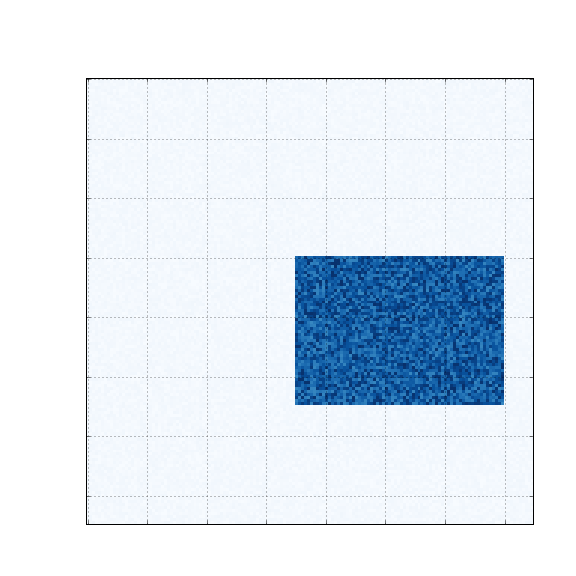
\includegraphics[width=\textwidth]{img/a-bic-structure.png}
        \caption{}
        \label{fig:bic-syntetic-structure:a}
    \end{subfigure}
    ~
    \begin{subfigure}[b]{0.18\textwidth}
        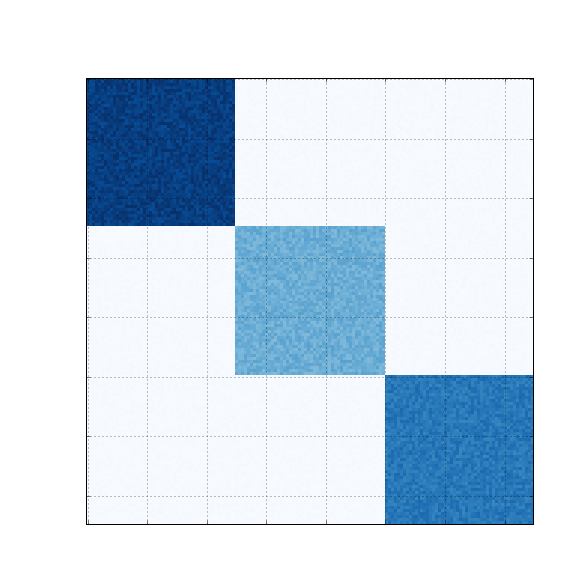
\includegraphics[width=\textwidth]{img/b-bic-structure.png}
        \caption{}
        \label{fig:bic-syntetic-structure:b}
    \end{subfigure}
    ~
    \begin{subfigure}[b]{0.18\textwidth}
        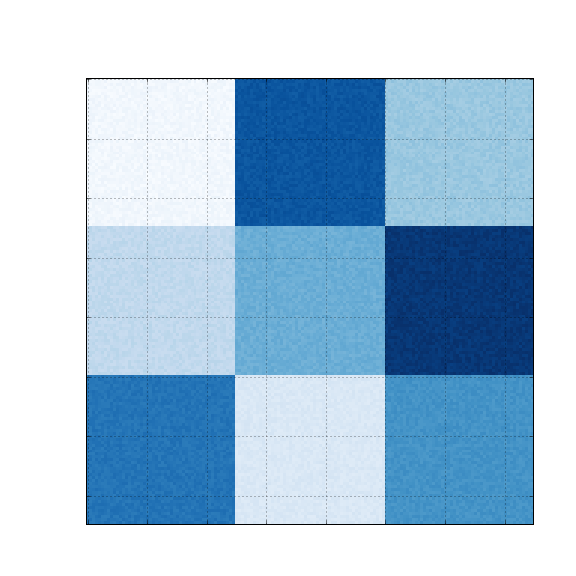
\includegraphics[width=\textwidth]{img/c-bic-structure.png}
        \caption{}
        \label{fig:bic-syntetic-structure:c}
    \end{subfigure}
    ~
    \begin{subfigure}[b]{0.18\textwidth}
        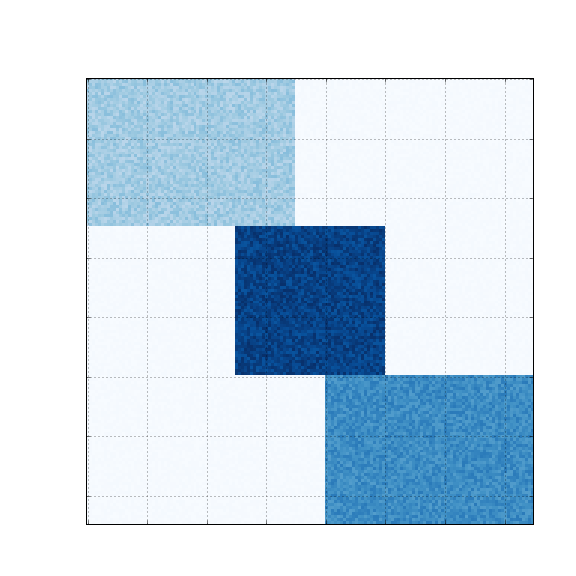
\includegraphics[width=\textwidth]{img/d-bic-structure.png}
        \caption{}
        \label{fig:bic-syntetic-structure:d}
    \end{subfigure}
    ~
    \begin{subfigure}[b]{0.18\textwidth}
        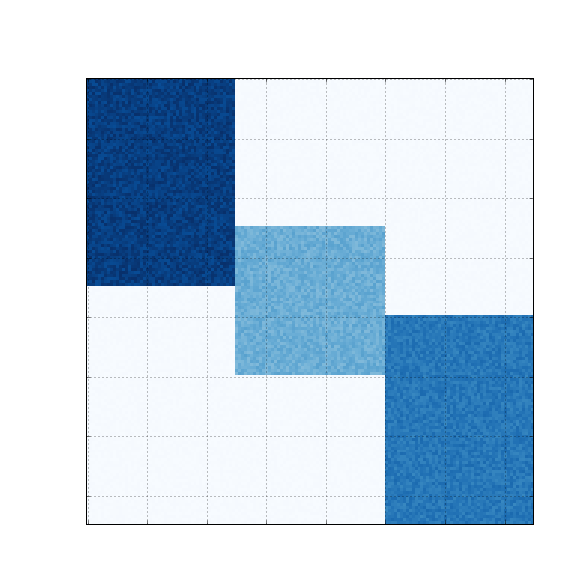
\includegraphics[width=\textwidth]{img/e-bic-structure.png}
        \caption{}
        \label{fig:bic-syntetic-structure:e}
    \end{subfigure}
    \label{fig:bic-syntetic-structure}
      \source{Lucas Fernandes Brunialti, 2016}
\end{figure}

% Sara: verificar se é cogrupo ou co-grupo
% Lucas: acho que podemos usar cogrupo, na literatura, tem gente que usa co-clustering e tem gente q usa cogrupoing

% Sara: talvez tenhamos que tratar cogrupo de interesse, pod conta da definição baseada em particionamento
% Lucas: Se usassemos bicluster para falar de encontrar submatriz e cogrupo fazer particionamento não teríamos esse problema
Para compreender a representação gráfica apresentada na figura~\ref{fig:bic-syntetic-structure} considere que cada um dos cinco quadrados maiores representa uma base de dados sintética, que a quantidade de dados da base está representada pela altura do quadrado, e que a quantidade de atributos na base está representada pela largura do quadrado.
Todas as bases de dados possuem $150$ dados (linhas) e $150$ atributos (colunas).
Considere ainda que cada quadrado ou retângulo, representados com diferentes tons da cor azul, representam um cogrupo, também com suas alturas e larguras representando, respectivamente, a quantidade de linhas e colunas que compõem cada cogrupo.
As diferentes tonalidades da cor azul revelam a similaridade entre os valores assumidos pelos dados em subconjuntos de atributos, o que também revela a existência dos cogrupos.
A intensidade da cor é proporcional à intensidade dos valores associados a cada atributo em cada dado, então valores maiores são representados por tonalidades mais escuras e vice-versa.
Por exemplo, a seguinte matriz poderia representar o caso da figura~\ref{fig:bic-syntetic-structure:b}, porém em dimensões menores que $150$ linhas por $150$ colunas:
\[
    \begin{bmatrix}
        \mathbf{30,3} & \mathbf{31,6} & \mathbf{30,9} & 1,0           & 0,8           & 0,9           & 0,7           & 0,7           & 0,1           \\
        \mathbf{29,1} & \mathbf{30,7} & \mathbf{30,0} & 0,7           & 0,0           & 0,6           & 0,8           & 0,1           & 0,9           \\
        \mathbf{30,8} & \mathbf{29,5} & \mathbf{31,5} & 0,2           & 0,7           & 0,2           & 0,9           & 0,7           & 0,5           \\
        0,4           & 0,9           & 1,0           & \mathbf{10,5} & \mathbf{9,2}  & \mathbf{10,8} & 0,8           & 0,8           & 0,8           \\
        0,5           & 0,7           & 0,5           & \mathbf{11,1} & \mathbf{10,0} & \mathbf{9,2}  & 0,9           & 0,7           & 0,6           \\
        0,3           & 0,4           & 0,5           & \mathbf{10,8} & \mathbf{11,2} & \mathbf{10,9} & 0,5           & 0,3           & 0,1           \\
        0,0           & 0,7           & 0,4           & 0,4           & 0,1           & 0,4           & \mathbf{20,2} & \mathbf{19,6} & \mathbf{20,4} \\
        0,8           & 0,5           & 1,0           & 0,4           & 0,7           & 0,3           & \mathbf{21,2} & \mathbf{20,7} & \mathbf{19,4} \\
        0,0           & 0,6           & 0,4           & 0,6           & 0,1           & 0,1           & \mathbf{19,9} & \mathbf{20,2} & \mathbf{20,9}
    \end{bmatrix}
\]

Todas as bases de dados da figura~\ref{fig:bic-syntetic-structure} são matrizes de valores reais positivos geradas artificialmente.
Primeiramente, uma matriz de tamanho $150 \times 150$ é preenchida com valores ponto flutuante, gerados aleatoriamente a partir de uma função $\mathcal{U}(0, 1)$, que gera números de uma distribuição uniforme no intervalo $]0, 1]$.
Em seguida, o tamanho em termo de linhas e colunas e disposição dos cogrupos na base de dados foram determinados de acordo com cada estrutura de cogrupos desejada.
Para instanciar cada cogrupo, um conjunto de valores foi criado e distribuído pelas células do cogrupo da seguinte forma:

% Todas as bases de dados da figura~\ref{fig:bic-syntetic-structure} são \textcolor{red}{matrizes de valores reais positivos} geradas artificialmente. Primeiramente, uma matriz de tamanho $150 \times 150$ é preenchida com valores ponto flutuante, gerados aleatoriamente a partir de uma distribuição uniforme $unif(0.0, 1.0)$, no intervalo $[0.0, 1.0]$\footnote{Este processo evita que ocorram divisões por $0$ nos algoritmos. \textcolor{red}{Que processo? O que exatamente evita? Ser positivo, ser uniforme? Sugiro que essa observação vá para um rodapé, mas precisa ser mais específica.}}. Em seguida, os cogrupos foram gerados a partir da escolha aleatória de um valor central $c \in \mathcal{C}$, sendo $\mathcal{C} = \{ 20, 40, 60, 80, 100, 120, 140, 160, 180 \}$, e da adição de valores gerados a partir da função $unif(0.0, 10.0)$ a elementos localizados a uma distância matricial \textcolor{red}{em um raio $a_1, a_2$ de $c$, respectivamente na direção das linhas e das colunas da matriz.}

\begin{itemize}
    \item um valor central $c \in \mathcal{C}$, sendo $\mathcal{C} = \{ 20, 40, 60, 80, 100, 120, 140, 160, 180 \}$, foi aleatoriamente escolhido, e retirado de $\mathcal{C}$ para não haver cogrupos com o mesmo $c$ em uma mesma matriz;
    \item o conjunto de valores usado para instanciar as células do cogrupo foi estabelecido por meio da adição de $c$ a valores reais, gerados a partir da função $\mathcal{U}(0, 10)$, que gera números de uma distribuição uniforme no intervalo $]0, 10]$;
    \item cada um dos valores nesse conjunto foi atribuído às células previamente definidas como pertecentes ao cogrupo.
\end{itemize}

Assim, considerando que um cogrupo é uma submatriz da matriz original $X$, ele pode ser gerado pela equação:
\[
    x_{ij} = c + \mathcal{U}(0, 10)
\]
sendo $i$ e $j$ os índices das linhas e colunas de $X$ escolhidos para compor o cogrupo.

Ainda sobre a interpretação da figura~\ref{fig:bic-syntetic-structure}, alguns detalhes precisam ser observados.
A depender do objetivo da análise de coagruamento, na figura~\ref{fig:bic-syntetic-structure:a}, por exemplo, mais de um cogrupo pode ser observado, além daquele que é de interesse de análise neste trabalho.
Para essa interpretação, considera-se que todo agrupamento de linhas e de colunas, independente de serem úteis ou não, ou de serem interessante para análise ou não, é um cogrupo.
Assim, tem-se os seguintes cogrupos na base de dados sintética (a):

% Conferir

\begin{itemize}
\item O mais evidente, destacado em azul, é formado pelas linhas [60, \dots, 109] e pelas colunas [70, \dots, 139]. Esse é o cogrupo de interesse, nesse projeto, para a resolução da tarefa de coagrupamento aplicada a dados textuais, e é representado na figura~\ref{fig:bic-syntetic-structure:a} pelo quadrado em cor azul.
\item O segundo, que não está destacado na visualização, é formado por todas as linhas e as colunas [0, \dots, 69] e [140, \dots, 149].
\item O terceiro, também não destacado, é formado por todas as colunas e as linhas [0, \dots, 59] e [110, \dots, 149].
\end{itemize}

Sob essa ótica de interpretação, as demais bases de dados possuem:

\begin{itemize}
\item (b): três cogrupos de principal interesse e seis cogrupos não destacados na figura;
\item (c): seis cogrupos de principal interesse;
\item (d): três cogrupos de principal interesse e oito cogrupos não destacados na figura;
\item (e): três cogrupos de principal interesse e oito cogrupos não destacados na figura.
\end{itemize}

% sugiro que seja colocada a descrição detalhada de cada um apenas se tivermos espaço, se o texto não ficar muito longo. Eventualmente, também podemos deixar em Apêndice, ou fazer uma figura também para cá ou para o Apêndice.

% ***************************************************************************
% ***************************************************************************

%Lucas, eu estou deixando o seu original mas estou propondo outra forma de descrever. Precisamos discutir qual delas vai ficar.

%\begin{itemize}
%    \item \textit{\textbf{Figura~\ref{fig:bic-syntetic-structure:a}}} há um bicluster, formado pelas linhas de $60$ à $110$ e pelas colunas de $70$ à $140$; sendo então, dois cogrupos de linhas, o primeiro formado pelas linhas de $60$ à $110$ e o segundo pelas demais linhas, e dois cogrupos de colunas, o primeiro formado pelas colunas de $70$ à $140$ e o segundo pelas demais colunas.
%    \item \textit{\textbf{Figura~\ref{fig:bic-syntetic-structure:b}}} há três biclusters sem intersecção, o primeiro formado pelas linhas de $0$ à $49$ e pelas colunas de $0$ à $49$, o segundo formado pelas linhas de $50$ à $99$ e pelas colunas $50$ à $99$, o terceiro formado pelas linhas de $100$ à $149$ e pelas colunas de $100$ à $149$; sendo então, três cogrupos de linhas sem intersecção e três cogrupos de colunas sem intersecção, o primeiro formado pelas linhas de $0$ à $49$, o segundo formado pelas linhas de $50$ à $99$, o terceiro formado pelas linhas de $100$ à $149$, o quarto formado pelas colunas de $0$ à $49$, o quinto formado pelas colunas de $50$ à $99$, e o sexto formado pelas colunas de $100$ à $149$, respectivamente.
%   Também existe outra forma de observar os cogrupos presentes neste caso, se for considerado os cogrupos de colunas para cada cogrupo de linhas, seriam os mesmos três cogrupos de linhas e dois cogrupos de colunas para cada cogrupo de linha, ou seja, para o primeiro cogrupo de linhas (linhas $0$ à $49$), os dois cogrupos de colunas são os cogrupos formados pelas colunas de $0$ à $49$ e pelas demais colunas ($50$ à $149$), seguindo a mesma lógica para os demais cogrupos.
%    Note que desta maneira, é possível que cogrupos de colunas tenham intersecção.
%    \item \textit{\textbf{Figura~\ref{fig:bic-syntetic-structure:c}}} há nove biclusters com intersecção em estrutura de xadrez, formados através da divisão da matriz de dados sintética em partes iguais; sendo assim, serão 3 cogrupos de linhas sem intersecção e 3 cogrupos de colunas sem intersecção, o primeiro formado pelas linhas de $0$ à $49$, o segundo formado pelas linhas de $50$ à $99$, o terceiro formado pelas linhas de $100$ à $149$, o quarto formado pelas colunas de $0$ à $49$, o quinto formado pelas colunas de $50$ à $99$, e o sexto formado pelas colunas de $100$ à $149$.
%    É possível fazer a mesma observação de cogrupos realizada no item \textit{\textbf{Figura~\ref{fig:bic-syntetic-structure:b}}}, totalizando nove cogrupos, três cogrupos de linhas e três cogrupos de colunas para cada cogrupo de linha.
%    \item \textit{\textbf{Figura~\ref{fig:bic-syntetic-structure:d}}} há três biclusters com intersecção nas colunas, o primeiro formado pelas linhas de $0$ à $49$ e pelas colunas de $0$ à $69$, o segundo formado pelas linhas de $50$ à $99$ e pelas colunas $50$ à $99$, e o terceiro formado pelas linhas de $100$ à $149$ e pelas colunas de $79$ à $149$; sendo então, 3 cogrupos de linhas sem intersecção e 3 cogrupos de colunas com intersecção.
%    Considerando os cogrupos de colunas para cada cogrupo de linhas, serão nove cogrupos, dois cogrupos de colunas para cada um dos três cogrupos de linhas.
%    \item \textit{\textbf{Figura~\ref{fig:bic-syntetic-structure:e}}} Este caso é exatamente igual ao item \textit{\textbf{Figura~\ref{fig:bic-syntetic-structure:d}}} se for observado a transposição da matriz de dados sintética.
% \end{itemize}

% ***************************************************************************
% ***************************************************************************

Para cada uma das bases de dados sintéticas foram executados os seguintes algoritmos: \textit{k-means}\footnote{Para os experimentos com \textit{k-means} foi usada a implementação da biblioteca \textit{scikit-learn}~\cite{scikitLearn} da linguagem Python.}, \textit{fuzzy k-means}\footnote{Para experimentos com \textit{fuzzy k-means} foi usado a implementação do algoritmo \textit{fuzzy k-means} da biblioteca \textit{scikit-fuzzy} da linguagem Python.}, \textit{ONMTF}, \textit{FNMTF}, \textit{OvNMTF} e \textit{BinOvNMTF}\footnote{Os algoritmos baseadas em fatoração de matrizes foram implementados pelo autor deste trabalho usando a linguagem Python.}.
Os resultados foram analisados em termos de qualidade de reconstrução e capacidade de quantização.

\subsection{Análise da reconstrução}

% para isso valer vamos ter que definir kmeans e fuzzy k means em termos de fatoração de matrizes; ou mudar um pouco essa frase aqui.
% porém, pela forma como foi explicado mais abaixo, acho que vamos ter que melhorar aqui já explicando aqui o que é a resconstruação para o kmeans e o fuzzy k means.
% Uma forma de analisar o resultado dos algoritmos estudados neste trabalho é analisá-los quanto a sua capacidade de reconstrução. Para os algoritmos baseados em fatoração de matrizes, a reconstrucão é feita tomando as matrizes resultantes da fatoração e combinando-as \textcolor{red}{da mesma forma que o seu problema foi proposto}, de forma a reconstruir a matriz original. \textcolor{red}{Para o caso dos algoritmos \textit{k-means} e \textit{fuzzy-k-means}, a resconstrução foi representada pela substituição do valor do centróide ....}

% Essa análise se torna importante a partir do momento em que se tem como objetivo avaliar o comportamento dos algoritmos em diferentes estruturas de organização de cogrupos. A capacidade de reconstrução .... \textcolor{red}{vamos ver se colocamos alguma coisa a mais para justificar esse análise.}
Uma forma de analisar o resultado dos algoritmos estudados neste trabalho é analisá-los quanto a sua capacidade de reconstrução.
A reconstrucão é feita tomando as matrizes resultantes da fatoração e combinando-as da mesma forma que o seu problema foi proposto, de forma a reconstruir a matriz original.

Essa análise se torna importante quando se tem como objetivo avaliar o comportamento dos algoritmos em diferentes estruturas de organização de cogrupos, com destaque para a análise de maior interesse neste trabalho -- coagrupamento com sobreposição parcial de linhas ou colunas.
% TODO Descrever melhor pq a reconstrução é importante
% Lucas: Não consigo pensar em algo impactante para colocar aqui
%  essa análise serve pra q? acho que para ver quais estruturas os algoritmos são capazes de detectar, assim, quando vc tiver um problema real, e a idéia de como esse problema esta estruturado, vc pode usar um algoritmo ou outro. Talvez isso seja um caminho...

Um resumo sobre os resultados obtidos nessa análise é apresentado na tabela~\ref{tab:resumoREC}.
O restante dessa seção se destina a detalhar as análise de qualidade de reconstrução.

\begin{table}[htpb]
\centering
    \caption{Resumo de qualidade de reconstrução: $ok$ - permite reconstrução de forma natural; $\times$ - sem informação sobre sobreposição parcial; $+$ - preserva informação de sobreposição parcial}
        \begin{tabular}{lccccc}
            \hline
            & \textbf{base (a)} & \textbf{base (b)} & \textbf{base (c)} & \textbf{base (d)}& \textbf{base (e)} \\
            \hline
            \textit{k-means}       & $ok$ & $ok$ & $ok$ & $ok, \times$ &     \\
            \textit{fuzzy k-means} & $ok$ & $ok$ & $ok$ & $ok, \times$ & $+$ \\
            \textit{ONMTF}         & $ok$ & $ok$ & $ok$ & $+$          & $+$ \\
            \textit{FNMTF}         & $ok$ & $ok$ & $ok$ &              &     \\
            \textit{OvNMTF}        & $ok$ & $ok$ & $ok$ & $ok, +$      & $ok, +$ \\
            \textit{BinOvNMTF}     & $ok$ & $ok$ & $ok$ & $ok, +       $ &   \\
            \hline
             & & & & &  \\
        \end{tabular}
    \label{tab:resumoREC}
    \source{Lucas Fernandes Brunialti, 2016}
\end{table}

\subsection{Reconstrução a partir dos resultados do algoritmo \textit{k-means}}
\label{subsec:results-reconstruction-kmeans}

% Sara: Lucas, verifique o erro mínimo buscado por favor, está estranho.
% Lucas: pq esta estranho?

Para execução dos experimentos com o \textit{k-means} os seguintes parâmetros foram estabelecidos: número máximo de iterações ($300$) ou a diferença do erro de quantização em duas iterações consecutivas ($\leq 1 \times 10^{-4}$), o que ocorrer primeiro, como critérios de parada; número de grupos $k = 2$ para a base de dados sintética (a) e $k = 3$ para as bases de dados sintéticas (b), (c), (d) e (e).
A escolha de $k$ foi realizada com a prerrogativa de que o algoritmo \textit{k-means} deveria encontrar os grupos considerando todos os atributos descritivos, e desta forma, agrupar os dados de acordo com a similaridade total. Assim, $k$ foi escolhido a partir da quantidade de agrupamento de linhas presente na base de dados.
A escolha de $k$ maiores levaria o algoritmo a, necessariamente, dividir em grupos diferentes os dados que deveriam pertencer a um mesmo agrupamento de linhas.
Foram executadas $10$ rodadas do algoritmo, com inicialização de centróides aleatória, sendo que o melhor modelo resultante nessas rodadas foi escolhido para ilustrar a avaliação da qualidade da reconstrução.

As reconstruções obtidas a partir dos centróides encontrados pelo algoritmo \textit{k-means} são ilustradas na figura~\ref{fig:reconstruction:kmeans}.
As matrizes originais são repetidas na figura, nas cinco primeiras posições, de forma a facilitar a análise visual dos resultados.
Para um melhor entendimento da representação gráfica, note que cada linha recebe cores de acordo com sua pertinência a um agrupamento de linhas (ou grupo, na visão de agrupamento) representado por um centróide.
Ou seja, se a linha $10$ pertencer ao centróide $1$, então os valores da linha $10$ serão substituídos pelos valores do centróide $1$.
Note que o centróide é um vetor com o mesmo número de coordenadas de um dado da base de dados, sendo assim, a substituição é direta.
O centróide que representa o agrupamento de linhas referente ao cogrupo de interesse (em azul na figura), possui, claramente, valores similares aos dados que pertencem a esse cogrupo, e por isso o procedimento proposto pode ser visto como uma representação de reconstrução.

\begin{figure}[H]
    \caption{
        As primeiras cinco matrizes são as matrizes originais, as demais são suas respectivas reconstruções, realizadas a partir dos resultados obtidos com o algoritmo \textit{k-means}.
    }
\centering
    \begin{subfigure}[b]{0.18\textwidth}
        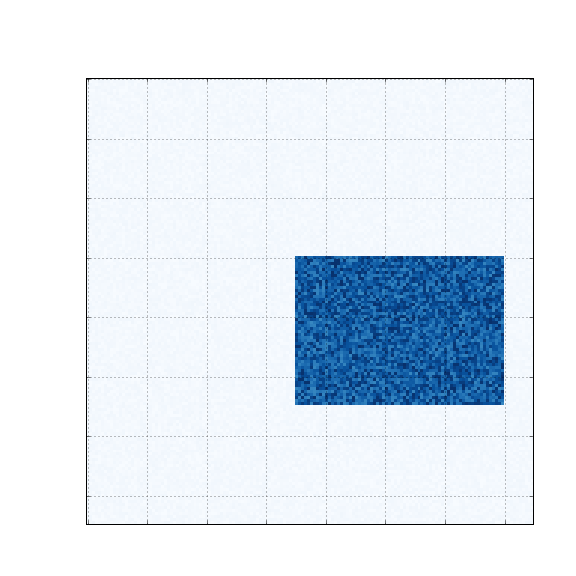
\includegraphics[width=\textwidth]{img/a-bic-structure.png}
    \end{subfigure}
    \begin{subfigure}[b]{0.18\textwidth}
        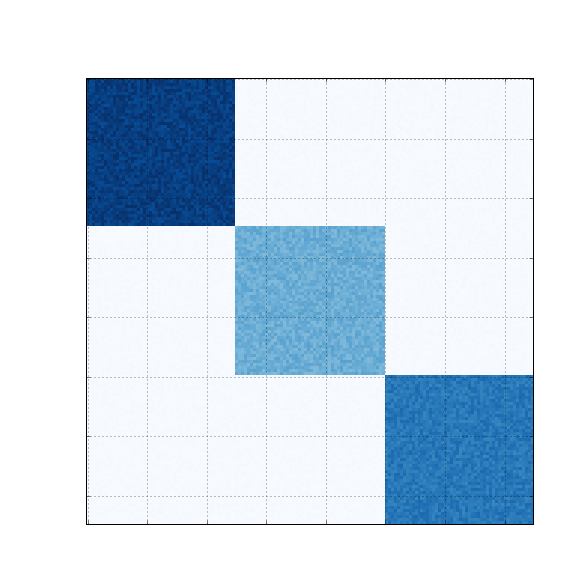
\includegraphics[width=\textwidth]{img/b-bic-structure.png}
    \end{subfigure}
    \begin{subfigure}[b]{0.18\textwidth}
        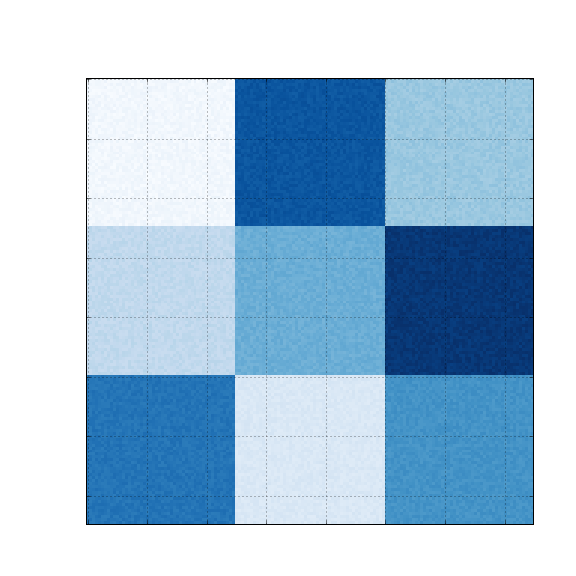
\includegraphics[width=\textwidth]{img/c-bic-structure.png}
    \end{subfigure}
    \begin{subfigure}[b]{0.18\textwidth}
        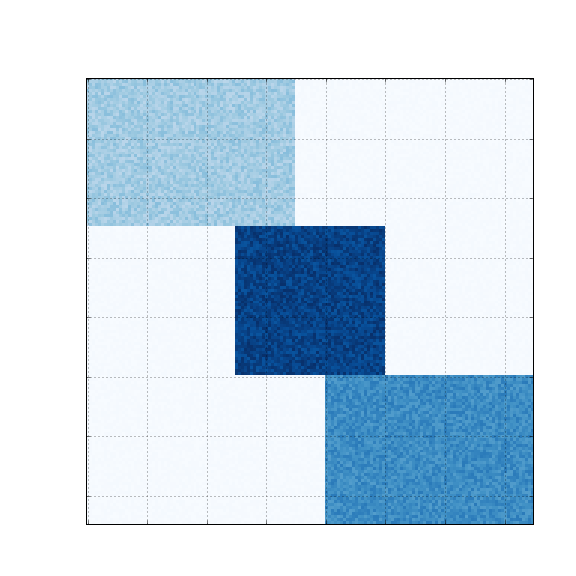
\includegraphics[width=\textwidth]{img/d-bic-structure.png}
    \end{subfigure}
    \begin{subfigure}[b]{0.18\textwidth}
        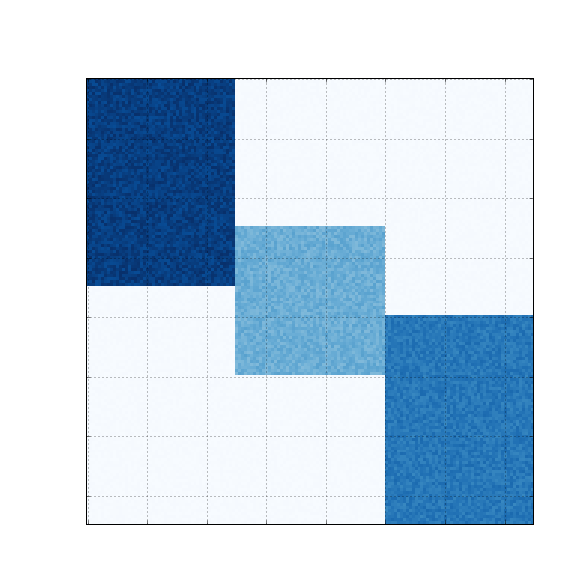
\includegraphics[width=\textwidth]{img/e-bic-structure.png}
    \end{subfigure}

    \begin{subfigure}[b]{0.18\textwidth}
        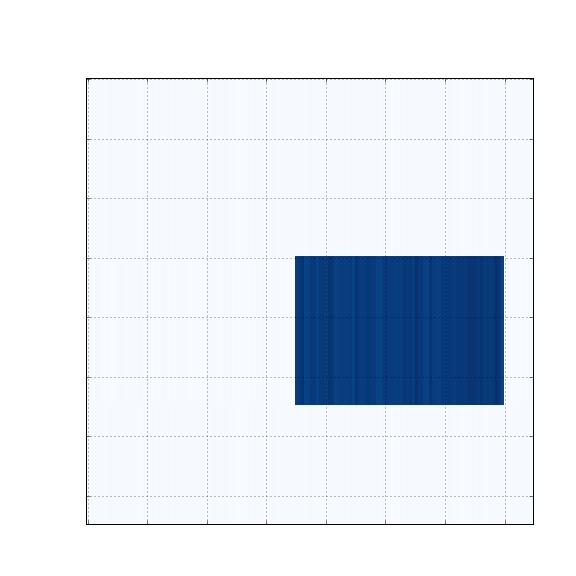
\includegraphics[width=\textwidth]{img/a-reconstruction-kmeans.png}
        \caption{}
    \end{subfigure}
    \begin{subfigure}[b]{0.18\textwidth}
        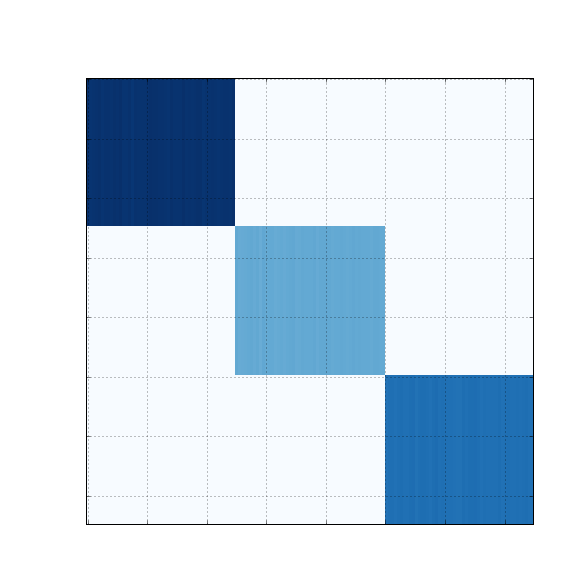
\includegraphics[width=\textwidth]{img/b-reconstruction-kmeans.png}
        \caption{}
    \end{subfigure}
    \begin{subfigure}[b]{0.18\textwidth}
        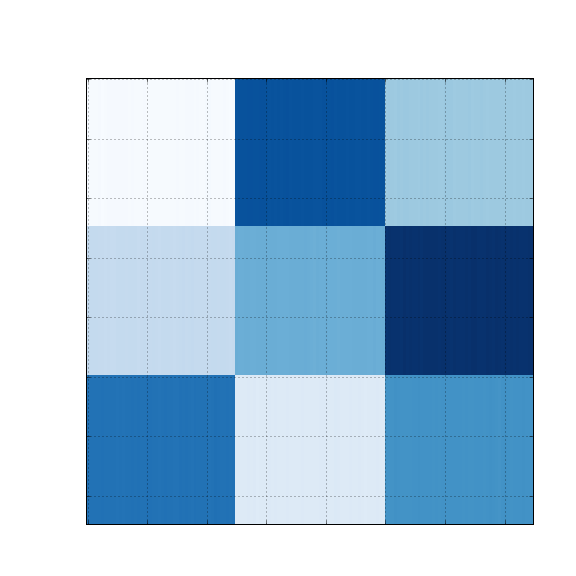
\includegraphics[width=\textwidth]{img/c-reconstruction-kmeans.png}
        \caption{}
    \end{subfigure}
    \begin{subfigure}[b]{0.18\textwidth}
        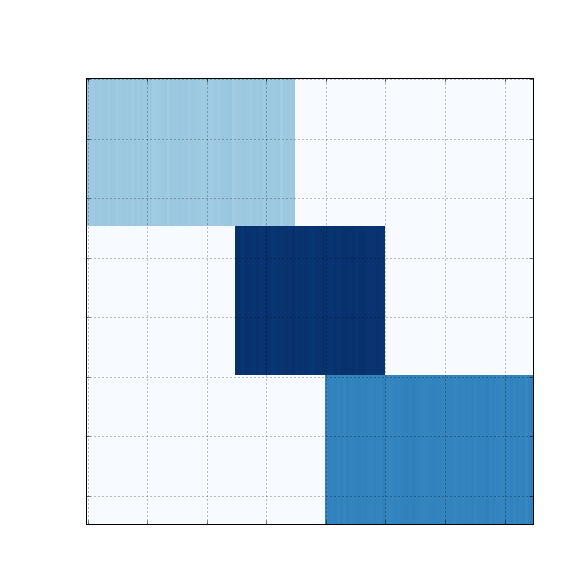
\includegraphics[width=\textwidth]{img/d-reconstruction-kmeans.png}
        \caption{}
    \end{subfigure}
    \begin{subfigure}[b]{0.18\textwidth}
        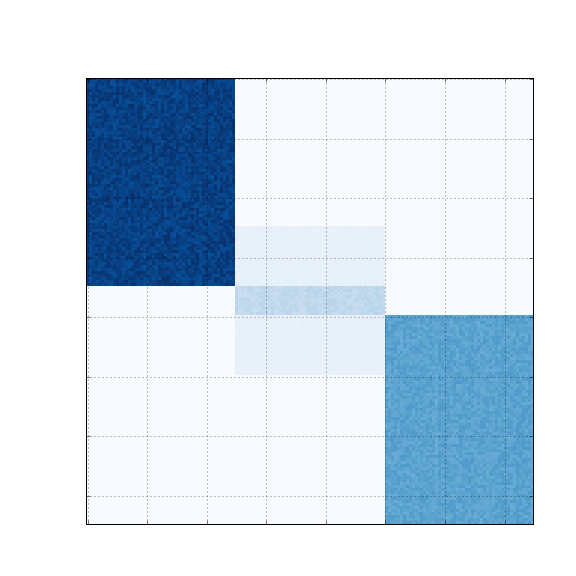
\includegraphics[width=\textwidth]{img/e-reconstruction-kmeans.png}
        \caption{}
    \end{subfigure}
    \label{fig:reconstruction:kmeans}
          \source{Lucas Fernandes Brunialti, 2016}
\end{figure}

% Sara: as cores não correspondem na reconstrução. Me lembro de isso ser devido a alguma normalização. Então precisa esclarecer aqui. Acho que uma nota de rodapé resolve.
% Lucas: como o centróide é a média dos valores, não tem como as cores corresponderem exatamente

O modelo resultante da execução do \textit{k-means} permite representar perfeitamente a reconstrução para as bases de dados (a) à (d).
Porém, é preciso lembrar que não há informação sobre agrupamento de colunas no resultado do algoritmo, sendo que a visualização gráfica de cada coagrupamento é possível apenas por conta do algoritmo levar em conta todos os atributos para realização do agrupamento.

O modelo não permite a descoberta de grupos com sobreposição de linhas (um dado não pode pertencer a mais de um grupo), e portanto não permite uma boa representação para a reconstrução no caso da base de dados (e).
Esse resultado já era esperado devido à natureza da solução apresentada pelo \textit{k-means}.

No entanto, se mudar o valor de $k$ para descobrir $5$ grupos ao invés dos $3$ grupos desejados, é possível realizar a reconstrução da base de dados (e), como mostra a figura~\ref{fig:reconstruction-2:kmeans}.
Porém, não é uma reconstrução natural, ou seja, a informação que seria desejado é que há $3$ grupos de linhas com sobreposição parcial entre o primeiro e o segundo grupos, e sobreposição parcial entre o segundo e terceiro grupos, diferentemente do obtido, que existe $5$ grupos diferentes.

\begin{figure}[H]
\centering
    \caption{Resultado da reconstrução da base de dados (e) utilizando o algoritmo \textit{k-means} com $k = 5$.}
    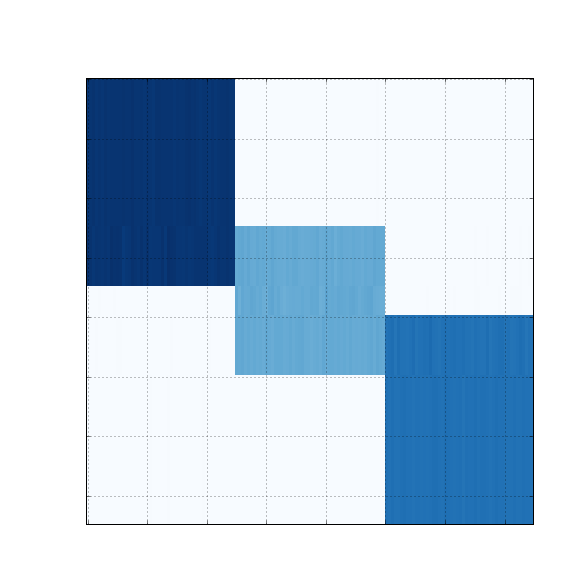
\includegraphics[width=0.3\textwidth]{img/e-reconstruction-2-kmeans.png}
    \label{fig:reconstruction-2:kmeans}
\source{Lucas Fernandes Brunialti, 2016}
\end{figure}

\subsection{Reconstrução a partir dos resultados do algoritmo \textit{fuzzy k-means}}
\label{subsec:results-reconstruction-fkmeans}

% verificar se podemos chamar de parâmetro de fuzzyficação
% Há uma justificativa para m=2, vamos colocar aqui.
% TODO eu li que esse é o usual (default), explicar pq
Os mesmos critérios de parada e número de grupos usados para o \textit{k-means} foram também usados nos experimentos com o \textit{fuzzy k-means}.
O valor para o parâmetro de fuzificação $m$ foi mantido em $2$, como indicado em \citeonline{Peres2012}.
Também, $10$ execuções foram realizadas, com iniciação aleatória de pesos e o melhor modelo obtido foi usado para avaliação da qualidade de reconstrução obtida.

% O parâmetro de fuzzyficação m é geralmente valorado com 2 para permitir que a pertinência de dados a grupos sejam obtidas unicamente em função das razões entre as distâncias entre dados e centros de grupos. Valores maiores do que 2 fazem com que as pertinências obtidas sejam influenciadas pela quantidade de grupos; valores menores do que 2 (se aproximando de 1, limite inferior para este parâmetro) aproxima o resultado do fuzzy-k-means do k-means pois as diferenças entre as pertinências tendem a aumentar.

As reconstruções apresentadas na figura~\ref{fig:reconstruction:fkmeans} foram obtidas por meio da multiplicação da matriz de partição pela matriz dos protótipos $UC$, resultantes da execução do algoritmo, e as matrizes originais foram repetidas para facilitar a análise visual.
Note que a matriz $U$ do \textit{fuzzy k-means} tem justamente o mesmo papel que a matriz de pertinências de linhas $U$ das fatorações \textit{BVD}, \textit{ONMTF} e \textit{OvNMTF}.

\begin{figure}[H]
\centering
    \caption{
        As primeiras cinco matrizes são as matrizes originais, as demais são suas respectivas reconstruções, realizadas a partir dos resultados obtidos com o algorimto \textit{fuzzy k-means}.
    }
    \begin{subfigure}[b]{0.18\textwidth}
        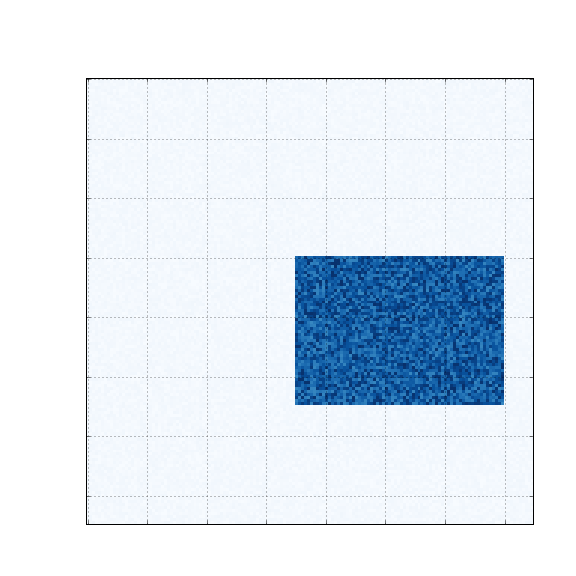
\includegraphics[width=\textwidth]{img/a-bic-structure.png}
    \end{subfigure}
    \begin{subfigure}[b]{0.18\textwidth}
        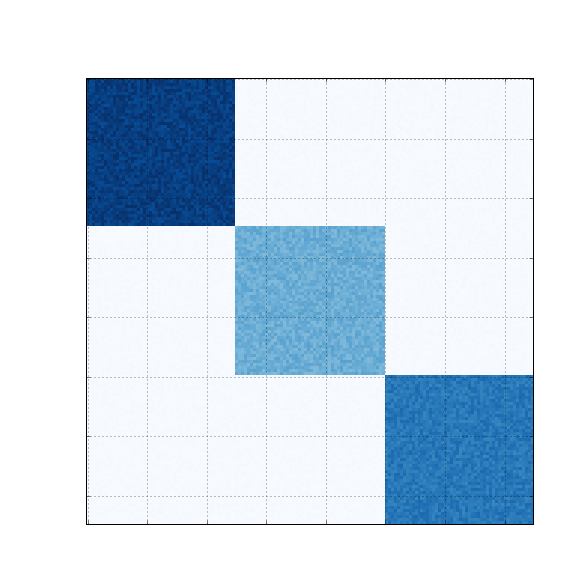
\includegraphics[width=\textwidth]{img/b-bic-structure.png}
    \end{subfigure}
    \begin{subfigure}[b]{0.18\textwidth}
        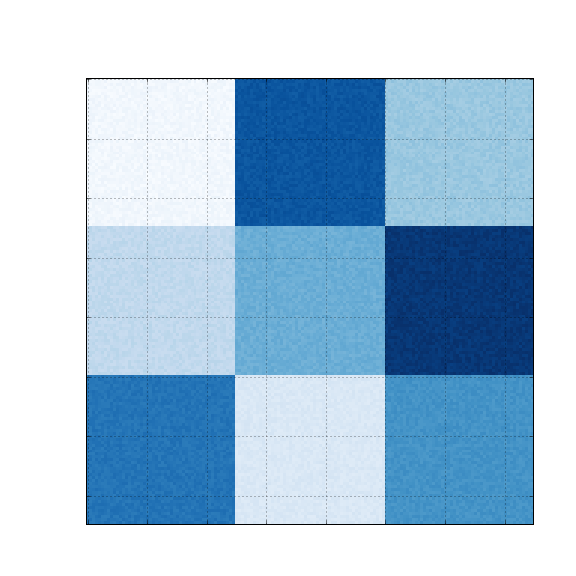
\includegraphics[width=\textwidth]{img/c-bic-structure.png}
    \end{subfigure}
    \begin{subfigure}[b]{0.18\textwidth}
        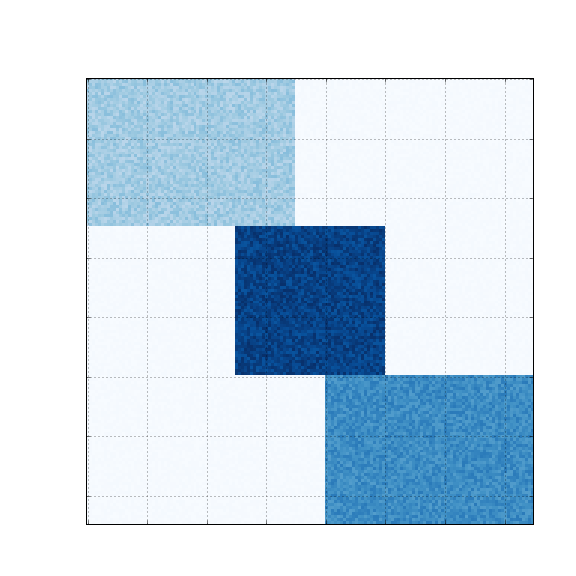
\includegraphics[width=\textwidth]{img/d-bic-structure.png}
    \end{subfigure}
    \begin{subfigure}[b]{0.18\textwidth}
        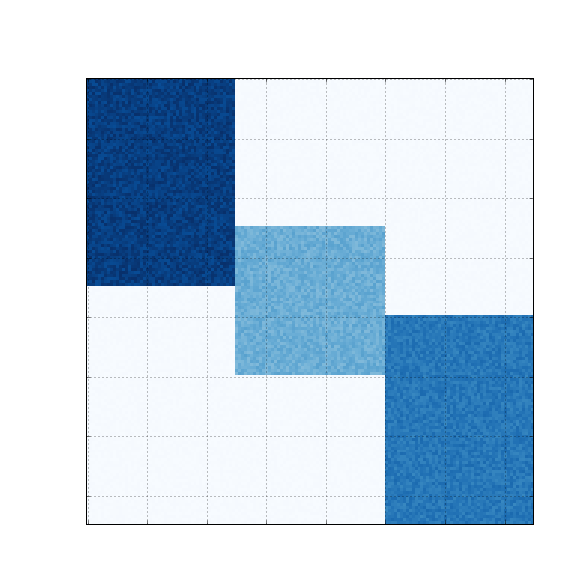
\includegraphics[width=\textwidth]{img/e-bic-structure.png}
    \end{subfigure}

    \begin{subfigure}[b]{0.18\textwidth}
        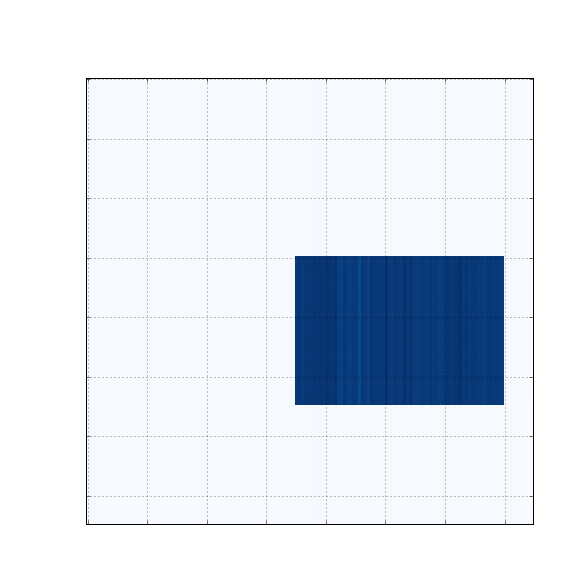
\includegraphics[width=\textwidth]{img/a-reconstruction-fkmeans.png}
        \caption{}
    \end{subfigure}
    \begin{subfigure}[b]{0.18\textwidth}
        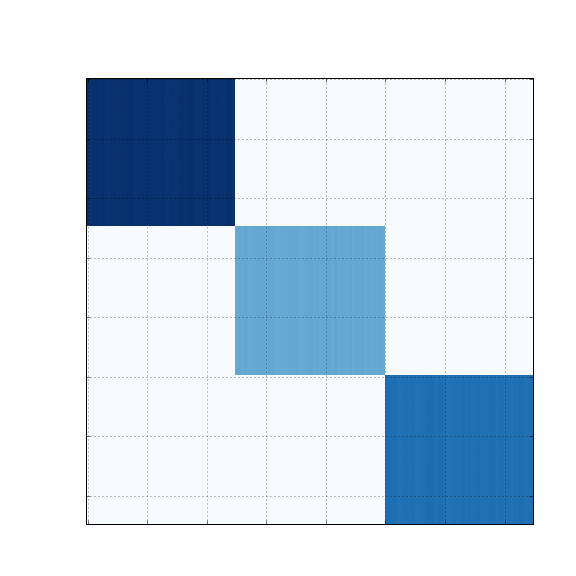
\includegraphics[width=\textwidth]{img/b-reconstruction-fkmeans.png}
        \caption{}
    \end{subfigure}
    \begin{subfigure}[b]{0.18\textwidth}
        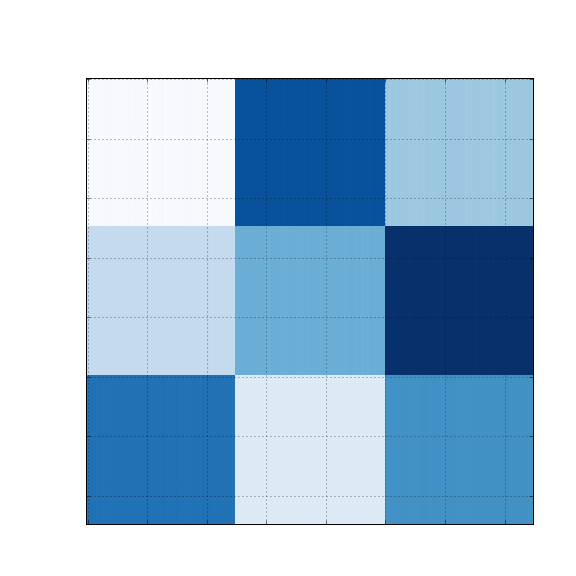
\includegraphics[width=\textwidth]{img/c-reconstruction-fkmeans.png}
        \caption{}
    \end{subfigure}
    \begin{subfigure}[b]{0.18\textwidth}
        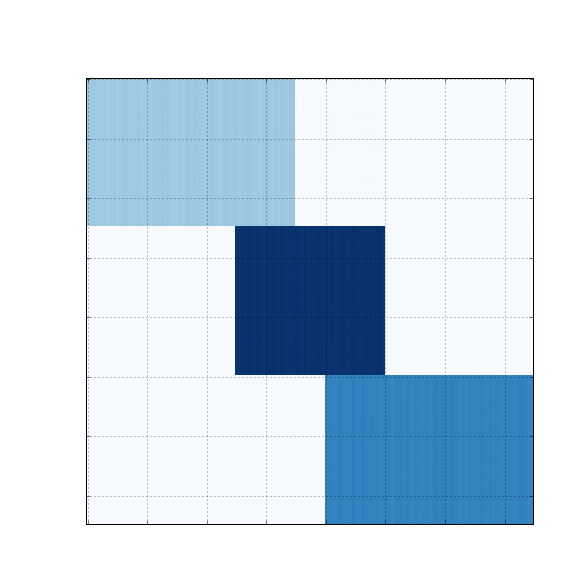
\includegraphics[width=\textwidth]{img/d-reconstruction-fkmeans.png}
        \caption{}
    \end{subfigure}
    \begin{subfigure}[b]{0.18\textwidth}
        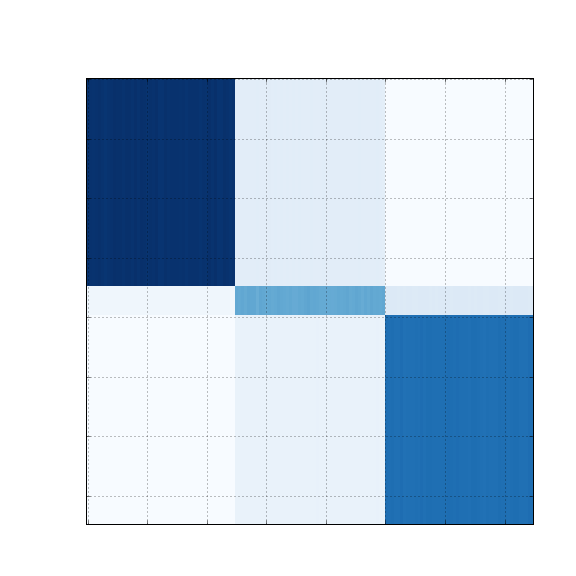
\includegraphics[width=\textwidth]{img/e-reconstruction-fkmeans.png}
        \caption{}
    \end{subfigure}
    \label{fig:reconstruction:fkmeans}
        \label{fig:reconstruction:kmeans}
\source{Lucas Fernandes Brunialti, 2016}
\end{figure}

% porém, apesar do algoritmo lidar com intersecção de clusters, este não foi capaz de fazer a reconstrução do caso (e).
% TODO dizer que no (e) foi pior que o kmeans?
% no kmeans parece que há uma variação dentro dos cogrupos que aqui não há. Seria interessante falar sobre isso?

% o caso E aqui está fazendo mais sentido que no kmeans e considerando a maior pertinência, deveria ser parecido no kmenas. Ou aqui seria melhor por indicar que há uma influencia diferentes naqueles atributos que tem algum coloracao, o que não kmeans não ocorre. Mas deveria ocorrer pois o centróide é media na coluna.

De forma semelhante à análise de reconstrução proporcionada pelo \textit{k-means}, o \textit{fuzzy k-means} também permite representar perfeitamente a reconstrução para as bases de dados (a) à (d).
Porém, a reconstrução para o caso (e) não foi obtida com sucesso.
No entanto, o algoritmo preservou parte da sobreposição, isso pode ser visto pelas regiões sombreadas onde há sobreposição de grupos.

% Embora o \textit{fuzzy c-means} lide, em sua concepção, com sobreposição de grupos, neste caso representada pelas pertinências fuzzy dos dados a vários grupos, o procedimento de escolha da maior pertinência anula essa capacidade na representação da reconstrução; \textcolor{blue}{muito embora .... é preciso fazer alguma ressalva ou análise diferente aqui.}

% aqui tem fuzzificação, verificar com Lucas. E se for feita com a segunda maior pertinência? Haverá alguma informação que complete a reconstrucão feita com a primeira???? Seria legal pensar nisso.

\begin{figure}[H]
\centering
    \caption{Resultado da reconstrução da base de dados (e) utilizando o algoritmo \textit{fuzzy k-means} com $k = 5$.}
    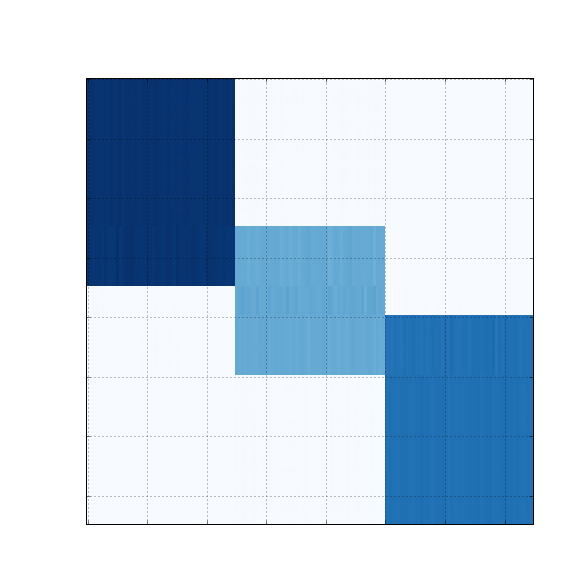
\includegraphics[width=0.3\textwidth]{img/e-reconstruction-2-fkmeans.png}
    \label{fig:reconstruction-2:fkmeans}
\source{Lucas Fernandes Brunialti, 2016}
\end{figure}

Da mesma forma que o \textit{k-means}, é possível mudar o valor de $k$ para $5$, para assim, obter uma reconstrução perfeita (Figura~\ref{fig:reconstruction-2:fkmeans}).
Fazendo as mesmas ressalvas, que a informação obtida a partir da interpretação desse modelo não é a desejada.

\subsection{Reconstrução a partir dos resultados do algoritmo \textit{ONMTF}}
\label{subsec:results-reconstruction-onmtf}

Para execução dos experimentos com o ONMTF a seguinte parametrização foi estabelecida: número máximo de iterações ($1000$) ou a diferença do erro de quantização em duas iterações consecutivas ($\leq 1 \times 10^{-4})$, o que ocorrer primeiro, como critérios de parada; o número de cogrupos de linhas ($k$) e colunas ($l$) configurados da seguinte maneira: $k = l = 2$ para (a) e $k = l = 3$ (b), (c), (d) e (e).
Novamente, as escolhas são baseadas no conhecimento \textit{apriori} que se tem sobre a quantidade de cogrupos, e quais cogrupos, deseja-se obter.
Para a visualização da reconstrução do algoritmo \textit{ONMTF} mantendo os valores (e portanto as cores) das matrizes de dados, não foi realizada a normalização baseada em probabilidade proposta por~\citeonline{Yoo2010} (apresentada no algoritmo~\ref{algo:onmtf2}), pois esta muda a escala dos valores da reconstrução, dada a interpretação probabilística que pode ser feita.

A partir da realização de $10$ execuções do algoritmo, foi escolhido o modelo que alcançou o menor erro de quantização, e a partir do resultado obtido a reconstrução foi avaliada.
A qualidade das resconstruções pode ser visualmente observada na figura~\ref{fig:reconstruction:onmtf}.
A resconstrução foi obtida a partir da multiplicação das matrizes fatoradas, ou seja, $USV^T$, conforme explicado no capítulo~\ref{ch:fatoracao}.

\begin{figure}[H]
\centering
    \caption{
        As primeiras cinco matrizes são as matrizes originais, as demais são suas respectivas reconstruções, realizadas a partir dos resultados obtidos com o algoritmo \textit{ONMTF}.
    }
    \begin{subfigure}[b]{0.18\textwidth}
        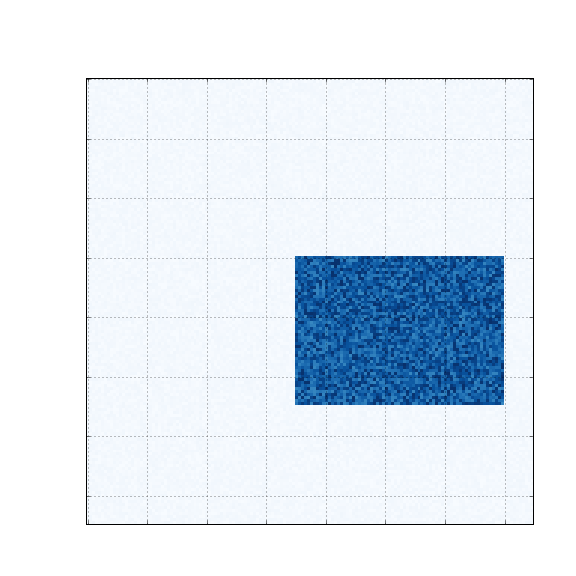
\includegraphics[width=\textwidth]{img/a-bic-structure.png}
    \end{subfigure}
    \begin{subfigure}[b]{0.18\textwidth}
        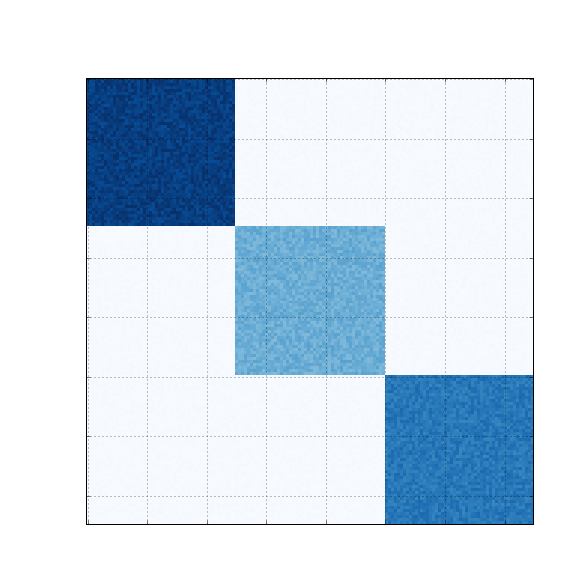
\includegraphics[width=\textwidth]{img/b-bic-structure.png}
    \end{subfigure}
    \begin{subfigure}[b]{0.18\textwidth}
        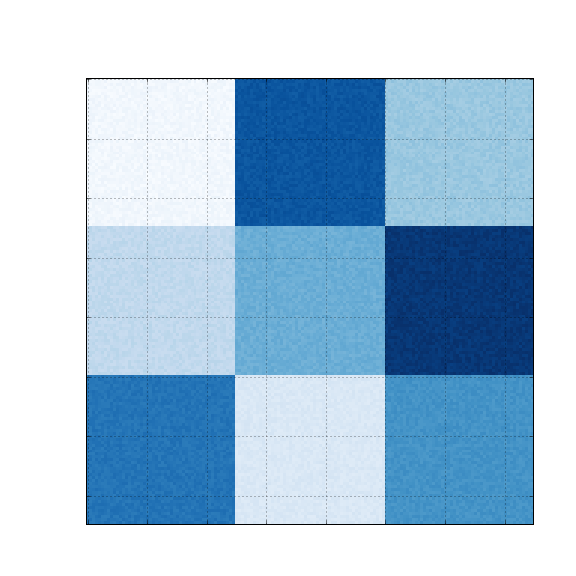
\includegraphics[width=\textwidth]{img/c-bic-structure.png}
    \end{subfigure}
    \begin{subfigure}[b]{0.18\textwidth}
        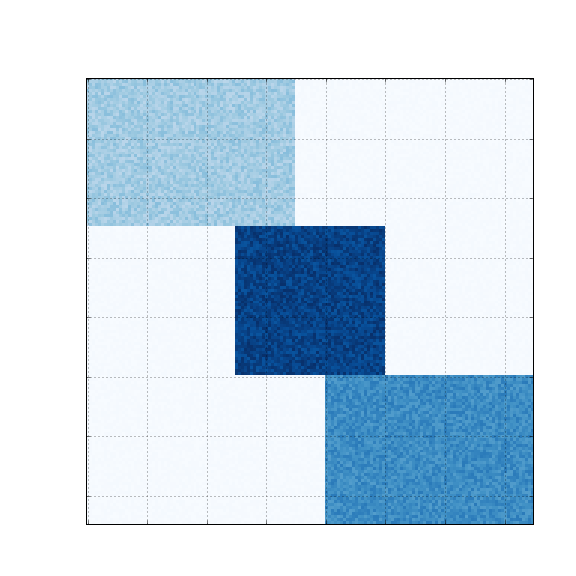
\includegraphics[width=\textwidth]{img/d-bic-structure.png}
    \end{subfigure}
    \begin{subfigure}[b]{0.18\textwidth}
        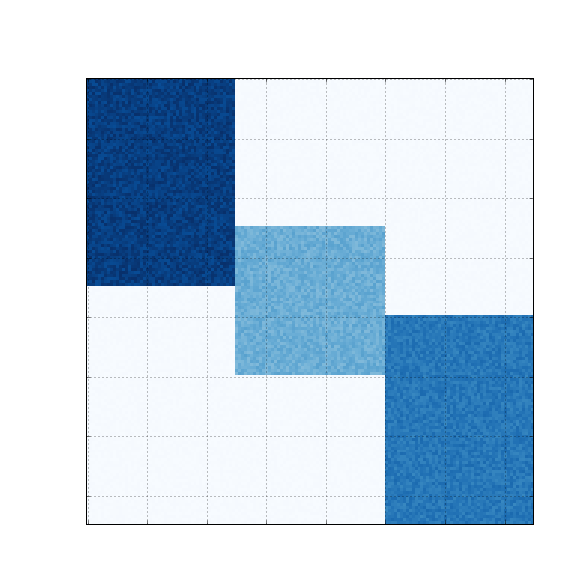
\includegraphics[width=\textwidth]{img/e-bic-structure.png}
    \end{subfigure}

    \begin{subfigure}[b]{0.18\textwidth}
        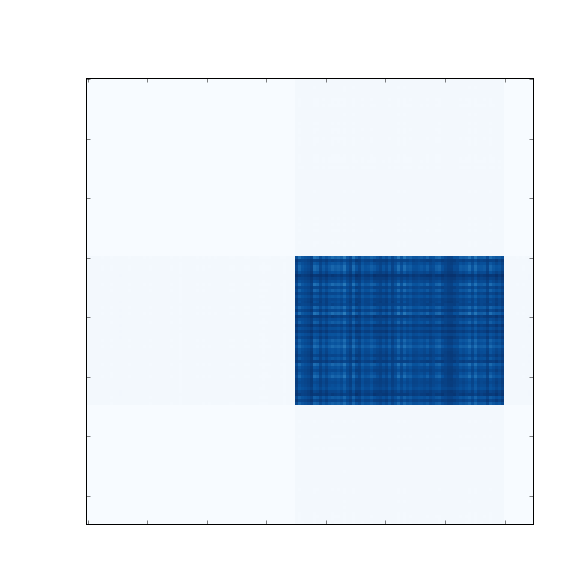
\includegraphics[width=\textwidth]{img/a-reconstruction-onmtf.png}
        \caption{}
    \end{subfigure}
    \begin{subfigure}[b]{0.18\textwidth}
        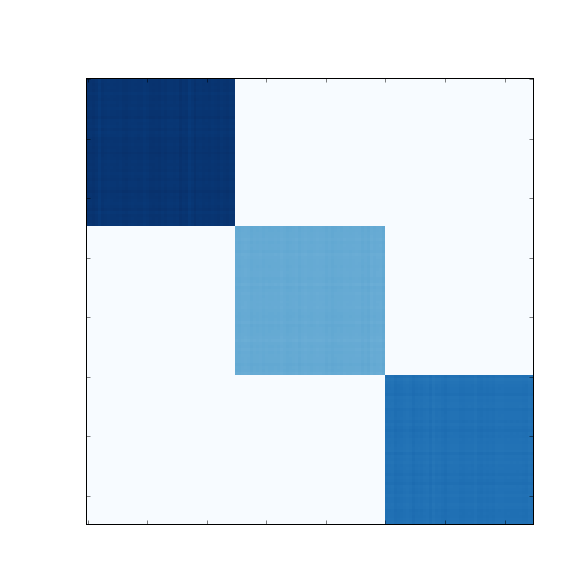
\includegraphics[width=\textwidth]{img/b-reconstruction-onmtf.png}
        \caption{}
    \end{subfigure}
    \begin{subfigure}[b]{0.18\textwidth}
        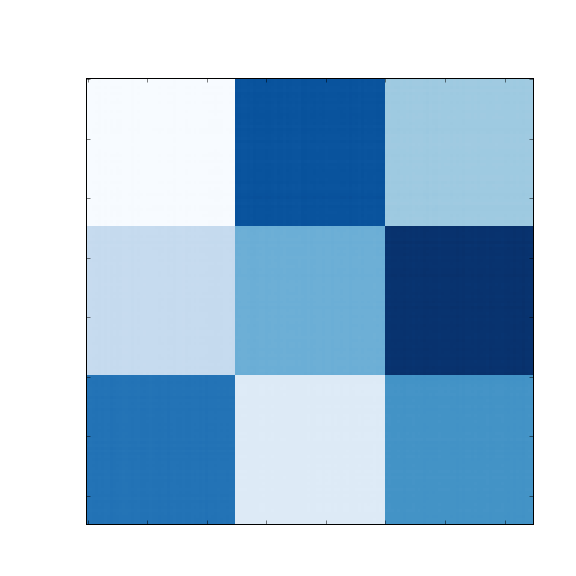
\includegraphics[width=\textwidth]{img/c-reconstruction-onmtf.png}
        \caption{}
    \end{subfigure}
    \begin{subfigure}[b]{0.18\textwidth}
        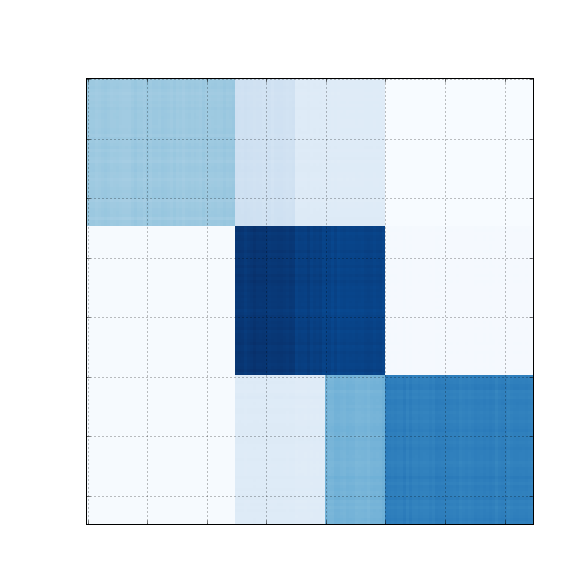
\includegraphics[width=\textwidth]{img/d-reconstruction-onmtf.png}
        \caption{}
    \end{subfigure}
    \begin{subfigure}[b]{0.18\textwidth}
        \includegraphics[width=\textwidth]{img/e-reconstruction-onmtf.png}
            \caption{}
    \end{subfigure}
\label{fig:reconstruction:onmtf}
\source{Lucas Fernandes Brunialti, 2016}
\end{figure}

% Sara: Aqui até as cores são identicas nos três primeiros casos. Não deveríamos ressaltar isso?
% Lucas: Como assim são idênticas? não vejo nesse nível de detalhe

Analisando os resultados, é possível perceber que a reconstrução é realizada com êxito nos casos (a), (b) e (c).
O algoritmo falhou em reconstruir a matriz no caso (d) pois não foi capaz de associar corretamente as colunas que pertencem a mais de um agrupamento de colunas (sobreposição parcial nas colunas).
O mesmo efeito ocorre com o caso (e), no qual há sobreposição parcial de linhas.
A falha da reconstrução é percebida na coloração diferenciada, formando regiões com sombras, nas colunas, ou linhas, envolvidas nas interseções.

A coloração diferenciada daquela esperada (seguindo a matriz original) é resultante do estado da matriz $V$, que contém as relações de associação de linhas e/ou colunas aos cogrupos.
Para o caso (d), por exemplo, é possível deduzir, a partir da análise visual, que há valores de magnitude diferentes estabelecendo a associação das colunas $50$ à $79$ e $80$ à $99$, que pertencem aos primeiro e terceiro cogrupos, respectivamente, com o cogrupo de colunas do meio.
Ou seja, a reconstrução preservou parte da sobreposição.
Esse comportamento é observado pois o algoritmo força a ortogonalidade entre cogrupos de linhas e cogrupos de colunas.

Ainda, é possível fazer a reconstrução perfeita, se mudar o valor de $l$ para 5 na base de dados (d), e o valor de $k$ para $5$ na base de dados (e) (Figura~\ref{fig:reconstruction-2:onmtf}).
Porém, como nos outros casos, a interpretação do modelo gerado não seria a desejada.

\begin{figure}[H]
\centering
    \caption{
        Resultado da reconstrução da base de dados (d) com $k = 5$ e (e) com $l = 5$, respectivamente, utilizando o algoritmo \textit{ONMTF}.
    }
    \begin{subfigure}[b]{0.18\textwidth}
        \includegraphics[width=\textwidth]{img/d-reconstruction-2-onmtf.png}
    \end{subfigure}
    \begin{subfigure}[b]{0.18\textwidth}
        \includegraphics[width=\textwidth]{img/e-reconstruction-2-onmtf.png}
    \end{subfigure}
\label{fig:reconstruction-2:onmtf}
\source{Lucas Fernandes Brunialti, 2016}
\end{figure}

\subsection{Reconstrução a partir dos resultados do algoritmo \textit{FNMTF}}
\label{subsec:results-reconstruction-fnmtf}

Para execução dos experimentos com o \textit{FNMTF} a seguinte parametrização foi estabelecida: número máximo de iterações ($300$) ou a diferença do erro de minimização em duas iterações consecutivas ($\leq 1 * 10^{-4}$), o que ocorrer primeiro, como critérios de parada; o número de cogrupos de linhas ($k$) e colunas ($l$) configurados da seguinte maneira: $k = l = 2$ para (a), $k = l = 3 $ para (b), (c), (d) e (e).

A partir da realização de $10$ execuções do algoritmo, foi escolhido o modelo que alcançou o menor erro de quantização, e a partir do resultado obtido a reconstrução foi avaliada.
A qualidade das reconstruções pode ser visualmente observada na figura~\ref{fig:reconstruction:fnmtf}.
A reconstrução foi obtida a partir da multiplicação das matrizes fatoradas, ou seja, $USV^T$, conforme explicado no capítulo~\ref{ch:fatoracao}.

\begin{figure}[H]
\centering
    \caption{
        As primeiras cinco matrizes são as matrizes originais, as demais são suas respectivas reconstruções, realizadas a partir dos resultados obtidos com o algoritmo \textit{FNMTF}.
    }
    \begin{subfigure}[b]{0.18\textwidth}
        \includegraphics[width=\textwidth]{img/a-bic-structure.png}
    \end{subfigure}
    \begin{subfigure}[b]{0.18\textwidth}
        \includegraphics[width=\textwidth]{img/b-bic-structure.png}
    \end{subfigure}
    \begin{subfigure}[b]{0.18\textwidth}
        \includegraphics[width=\textwidth]{img/c-bic-structure.png}
    \end{subfigure}
    \begin{subfigure}[b]{0.18\textwidth}
        \includegraphics[width=\textwidth]{img/d-bic-structure.png}
    \end{subfigure}
    \begin{subfigure}[b]{0.18\textwidth}
        \includegraphics[width=\textwidth]{img/e-bic-structure.png}
    \end{subfigure}

    \begin{subfigure}[b]{0.18\textwidth}
        \includegraphics[width=\textwidth]{img/a-reconstruction-fnmtf.png}
        \caption{}
    \end{subfigure}
    \begin{subfigure}[b]{0.18\textwidth}
        \includegraphics[width=\textwidth]{img/b-reconstruction-fnmtf.png}
        \caption{}
    \end{subfigure}
    \begin{subfigure}[b]{0.18\textwidth}
        \includegraphics[width=\textwidth]{img/c-reconstruction-fnmtf.png}
        \caption{}
    \end{subfigure}
    \begin{subfigure}[b]{0.18\textwidth}
        \includegraphics[width=\textwidth]{img/d-reconstruction-fnmtf.png}
        \caption{}
    \end{subfigure}
    \begin{subfigure}[b]{0.18\textwidth}
        \includegraphics[width=\textwidth]{img/e-reconstruction-fnmtf.png}
    \caption{}
    \end{subfigure}
    \label{fig:reconstruction:fnmtf}
\source{Lucas Fernandes Brunialti, 2016}
\end{figure}

Este caso é semelhante ao anterior (algoritmo \textit{ONMTF}).
O algoritmo permitiu a reconstrução com êxito dos casos (a), (b) e (c), falhando na reconstrução dos casos (d) e (e), nos quais há sobreposição de colunas ou linhas nos cogrupos de interesse. No entanto, nesse caso o algoritmo restringe a associação de linhas (ou colunas), a apenas um agrupamento de linhas (ou de colunas), e por isso a informação referente a sobreposição em cogrupos é totalmente descaracterizada.
Observe, por exemplo, que a reconstrução no caso (d) se assemelha à reconstrução do caso (c), embora as matrizes originais, em cada caso, representem informação sobre associação de dados e atributos em cogrupos também diferenciada.

Ainda, é possível fazer a reconstrução perfeita, se mudar o valor de $l$ para 5 na base de dados (d), e o valor de $k$ para $5$ na base de dados (e) (Figura~\ref{fig:reconstruction-2:onmtf}).
Porém, como nos outros casos, a interpretação do modelo gerado não seria a desejada.

\begin{figure}[H]
\centering
    \caption{
        Resultado da reconstrução da base de dados (d) com $k = 5$ e (e) com $l = 5$, respectivamente, utilizando o algoritmo \textit{FNMTF}.
    }
    \begin{subfigure}[b]{0.18\textwidth}
        \includegraphics[width=\textwidth]{img/d-reconstruction-2-fnmtf.png}
    \end{subfigure}
    \begin{subfigure}[b]{0.18\textwidth}
        \includegraphics[width=\textwidth]{img/e-reconstruction-2-fnmtf.png}
    \end{subfigure}
\label{fig:reconstruction-2:fnmtf}
\source{Lucas Fernandes Brunialti, 2016}
\end{figure}

\subsection{Reconstrução a partir dos resultados do algoritmo \textit{OvNMTF}}
\label{subsec:results-reconstruction-ovnmtf}

Para execução dos experimentos com o \textit{OvNMTF} a seguinte parametrização foi estabelecida: número máximo de iterações ($1000$) ou a diferença do erro de quantização ($\leq 1*10^{-4}$), o que ocorrer primeiro, como critérios de parada; o número de cogrupos de linhas ($k$) e colunas ($l$) configurados da seguinte maneira: $k = l = 2$ para (a), $k = 3$ e $l = 2 $ para (b), (d) e (e), e $k = l = 3$ para (c).
Note que o parâmetro $l$ mudou em relação às outras reconstruções, pois no caso dos algoritmos propostos, para escolher o parâmetro $l$, é necessário responder a pergunta: quantos cogrupos de coluna existem para cada cogrupo de linhas?

% TODO Sara: isso está repetindo muito, e a normalização e parametrizácão também, eu acho que é melhor colocar tudo no começo, ou em uma tabela. Acertar isso depois.
A partir da realização de $10$ execuções do algoritmo, foi escolhido o modelo que alcançou o menor erro de quantização, e a partir do resultado obtido a reconstrução foi avaliada.
A qualidade das reconstruções pode ser visualmente observada na figura~\ref{fig:reconstruction:ovnmtf}.
A reconstrução foi obtida a partir da multiplicação das matrizes fatoradas, ou seja, $U \sum_{p=1}^{k} I_{(p)} S V_{(p)}^T$, conforme explicado no capítulo~\ref{ch:proposedalgs}.



\begin{figure}[H]
\centering
    \caption{
        As primeiras cinco matrizes são as matrizes originais, as demais são suas respectivas reconstruções, realizadas a partir dos resultados obtidos com o algoritmo \textit{OvNMTF}.
    }
    \begin{subfigure}[b]{0.18\textwidth}
        \includegraphics[width=\textwidth]{img/a-bic-structure.png}
    \end{subfigure}
    \begin{subfigure}[b]{0.18\textwidth}
        \includegraphics[width=\textwidth]{img/b-bic-structure.png}
    \end{subfigure}
    \begin{subfigure}[b]{0.18\textwidth}
        \includegraphics[width=\textwidth]{img/c-bic-structure.png}
    \end{subfigure}
    \begin{subfigure}[b]{0.18\textwidth}
        \includegraphics[width=\textwidth]{img/d-bic-structure.png}
    \end{subfigure}
    \begin{subfigure}[b]{0.18\textwidth}
        \includegraphics[width=\textwidth]{img/e-bic-structure.png}
    \end{subfigure}

    \begin{subfigure}[b]{0.18\textwidth}
        \includegraphics[width=\textwidth]{img/a-reconstruction-ovnmtf.png}
        \caption{}
    \end{subfigure}
    \begin{subfigure}[b]{0.18\textwidth}
        \includegraphics[width=\textwidth]{img/b-reconstruction-ovnmtf.png}
        \caption{}
    \end{subfigure}
    \begin{subfigure}[b]{0.18\textwidth}
        \includegraphics[width=\textwidth]{img/c-reconstruction-ovnmtf.png}
        \caption{}
    \end{subfigure}
    \begin{subfigure}[b]{0.18\textwidth}
        \includegraphics[width=\textwidth]{img/d-reconstruction-ovnmtf.png}
        \caption{}
    \end{subfigure}
    \begin{subfigure}[b]{0.18\textwidth}
        \includegraphics[width=\textwidth]{img/e-reconstruction-ovnmtf.png}
        \caption{}
    \end{subfigure}
    \label{fig:reconstruction:ovnmtf}
\source{Lucas Fernandes Brunialti, 2016}
\end{figure}

O algoritmo conseguiu realizar a reconstrução com êxito em todos os casos.
Note que o algoritmo \textit{OvNMTF} é capaz de lidar com cogrupos com sobreposição de colunas, e portanto é capaz de resolver o caso (d).
Ainda, como não há restrições de ortogonalidade e existe fatores para controlar a pertinência de uma mesma linha ou coluna à multiplos cogrupos, o algoritmo é capaz de recontruir perfeitamente a base de dados (e).

\subsection{Reconstrução a partir dos resultados do algoritmo \textit{Bin\-OvNMTF}}
\label{subsec:results-reconstruction-binovnmtf}

Para execução dos experimentos com o \textit{BinOvNMTF} a seguinte parametrização foi estabelecida: número máximo de iterações ($300$) ou a diferença do erro de quantização ($\leq 1 * 10^{-4}$), o que ocorrer primeiro, como critérios de parada; o número de cogrupos de linhas ($k$) e colunas ($l$) configurados da mesma maneira que a reconstrução com o algoritmo \textit{OvNMTF}: $k = l = 2$ para (a), $k = 3$ e $l = 2$ para (b), (d) e (e), e $k = l = 3$ para (c).

A partir da realização de $10$ execuções do algoritmo, foi escolhido o modelo que alcançou o menor erro de quantização, e a partir do resultado obtido a reconstrução foi avaliada. A qualidade das reconstruções pode ser visualmente observada na figura~\ref{fig:reconstruction:binovnmtf}. A reconstrução foi obtida a partir da multiplicação das matrizes fatoradas, ou seja, $U \sum_{p=1}^{k} I_{(p)} S V_{(p)}^T$, conforme explicado no capítulo~\ref{ch:proposedalgs}.

\begin{figure}[H]
\centering
    \caption{
        As primeiras cinco matrizes são as matrizes originais, as demais são suas respectivas reconstruções, realizadas a partir dos resultados obtidos com o algoritmo \textit{BinOvNMTF}.
    }
    \begin{subfigure}[b]{0.18\textwidth}
        \includegraphics[width=\textwidth]{img/a-bic-structure.png}
    \end{subfigure}
    \begin{subfigure}[b]{0.18\textwidth}
        \includegraphics[width=\textwidth]{img/b-bic-structure.png}
    \end{subfigure}
    \begin{subfigure}[b]{0.18\textwidth}
        \includegraphics[width=\textwidth]{img/c-bic-structure.png}
    \end{subfigure}
    \begin{subfigure}[b]{0.18\textwidth}
        \includegraphics[width=\textwidth]{img/d-bic-structure.png}
    \end{subfigure}
    \begin{subfigure}[b]{0.18\textwidth}
        \includegraphics[width=\textwidth]{img/e-bic-structure.png}
    \end{subfigure}

    \begin{subfigure}[b]{0.18\textwidth}
        \includegraphics[width=\textwidth]{img/a-reconstruction-binovnmtf.png}
        \caption{}
    \end{subfigure}
    \begin{subfigure}[b]{0.18\textwidth}
        \includegraphics[width=\textwidth]{img/b-reconstruction-binovnmtf.png}
        \caption{}
    \end{subfigure}
    \begin{subfigure}[b]{0.18\textwidth}
        \includegraphics[width=\textwidth]{img/c-reconstruction-binovnmtf.png}
        \caption{}
    \end{subfigure}
    \begin{subfigure}[b]{0.18\textwidth}
        \includegraphics[width=\textwidth]{img/d-reconstruction-binovnmtf.png}
        \caption{}
    \end{subfigure}
    \begin{subfigure}[b]{0.18\textwidth}
        \includegraphics[width=\textwidth]{img/e-reconstruction-binovnmtf.png}
        \caption{}
    \end{subfigure}
    \label{fig:reconstruction:binovnmtf}
    \source{Lucas Fernandes Brunialti, 2016}
\end{figure}

O algoritmo \textit{BinOvNMTF} conseguiu realizar a reconstrução com êxito dos casos (a), (b), (c) e (d).
Como o algoritmo é capaz de lidar com cogrupos com sobreposição de colunas, ele é capaz de resolver o caso (d).
No entanto, o algoritmo não é capaz de lidar com cogrupos com sobreposição nas linhas, então, não é capaz de realizar a reconstrução do caso (e).
E nesse caso, também não preserva qualquer informação sobre a sobreposição, já que possui a restrição de associação binária (cada linha/coluna associadas a um único agrupamento de linhas/colunas).

Ao contrário dos algoritmos \textit{kmeans}, \textit{fuzzy kmeans}, \textit{ONMTF} e \textit{FNMTF}, não é possível fazer a reconstrução perfeita utilizando $k = 5$ para a base de dados (e) (Figura~\ref{fig:reconstruction-2:binovnmtf}).
Uma possível explicação para isso é que o algoritmo, dada todas as suas restrições, é incapaz de encontrar a solução que permite a reconstrução perfeita para a base de dados (e).

% -------------------------------------------------------------
\begin{figure}[H]
\centering
    \caption{Resultado da reconstrução da base de dados (e) utilizando o algoritmo \textit{Bin\-OvNMTF} com $k = 5$.}
    \includegraphics[width=0.3\textwidth]{img/e-reconstruction-2-binovnmtf.png}
    \label{fig:reconstruction-2:binovnmtf}
\source{Lucas Fernandes Brunialti, 2016}
\end{figure}

\subsection{Análise da capacidade de quantização}

Nos experimentos com as bases de dados sintéticas, fazendo o uso da mesma parametrização descrita para a análise da reconstrução, foi feita a medida do erro de quantização. A tabela~\ref{tab:quantization} sumariza o melhor erro de quantização resultante das $10$ execuções de cada algoritmo para cada base de dados.

% Lucas: Eu coloquei o \textit{BVD} aqui para mostrar que ele também consegue quantizar as matrizes perfeitamente!

\begin{table}[H]
\centering
    \caption{Avaliação da capacidade de quantização segundo o erro de quantização com os melhores destacados em negrito.}
        \begin{tabular}{lccccc}
            \hline
            & \textbf{base (a)} & \textbf{base (b)} & \textbf{base (c)} & \textbf{base (d)} & \textbf{base (e)} \\
            \hline
            \textit{k-means}        & $30.336,0$ & $62.776,5$ & $184.992,8$ & $\mathbf{79.238,5}$  & $2.886.245,5$        \\

            \textit{fuzzy k-means}  & $29.402,8$ & $63.768,5$ & $183.991,4$ & $\mathbf{78.340,0}$  & $2.307.168,6$        \\

           % \textit{BVD}            & $29.260,7$ & $61.536,5$ & $179.804,0$ & $\mathbf{75.575,0}$  & $\mathbf{77.135,5}$  \\

            \textit{ONMTF}          & $30.555,4$ & $60.794,8$ & $184.255,9$ & $579.136,7$          & $781.131,6$          \\

            \textit{FNMTF}          & $30.924,7$ & $64.636,1$ & $186.224,4$ & $1.634.328,5$        & $2.881.172,0$        \\

            \textit{OvNMTF}         & $30.439,8$ & $61.863,2$ & $178.886,8$ & $\mathbf{75.533,6}$  & $\mathbf{75.931,2}$  \\

            \textit{BinOvNMTF}      & $31.239,0$ & $63.660,4$ & $187.579,8$ & $\mathbf{79.968,0}$  & $3.160.391,0$        \\
            \hline \\
        \end{tabular}
        \label{tab:quantization}
        \source{Lucas Fernandes Brunialti, 2016}
\end{table}

Através dos resultados obtidos é possível perceber que a capacidade de quantização para todos os algoritmos para as bases de dados (a), (b) e (c), são semelhantes, assim como foi percebido na análise da reconstrução.

Para a base de dados (d), que contém cogrupos de colunas organizados com sobreposição parcial, os algoritmos que obtiveram erro de quantização entre $75.000$ e $80.000$ foram destacados na tabela~\ref{tab:quantization}, isso indica que eles foram capazes de quantizar a informação de sobreposição parcial.
É importante perceber que capacidade de quantização é diferente da possibilidade de interpretação da quantização realizada, isto é, os algoritmos \textit{kmeans} e \textit{fuzzy k-means} foram capazes de quantizar a sobreposição parcial de cogrupos de colunas, mas isso não quer dizer que é possível interpretar essa informação.
Como foi mostrado na análise de reconstrução, o algoritmo \textit{ONMTF} não quantizou toda a informação de sobreposição parcial da base de dados (d), mas parte dessa informação foi quantizada, diferentemente do algoritmo \textit{FNMTF}, que perdeu totalmente essa informação.
Isso também esta evidenciado na diferença do erro de quantização entre os algoritmos \textit{ONMTF} e \textit{FNMTF}.

O único algoritmo que foi capaz de quantizar a sobreposição parcial entre cogrupos de linhas da base de dados (e) foi o \textit{OvNMTF}, isso ocorre pois não há restrição de ortogonalidade entre cogrupos.
Da mesma forma que na base de dados (d), o algoritmo \textit{ONMTF} não quantizou toda a informação de sobreposição, evidenciado pela diferença do erro de quantização obtido pelo algoritmo \textit{OvNMTF}.


% Lucas: Essa subseção acho q não faz mais sentido, mas eu vou deixar comentada
% ===========================================================
% \subsection{Análise de particionamento}
% % TODO: Comparar reconstrução com dados da tabela

% % <<<<<<< HEAD
% % A análise de particionamento avaliada nesta seção diz respeito ao entendimento do quanto os grupos de linhas formados estariam adequados em relação a um modelo conhecido \textit{apriori}. Os mesmos modelos que foram analisado quanto à qualidade de reconstrução, foram usados para a análise apresentada aqui. Como os as bases de dados foram sintetizadas, foi possível rotulá-las de forma que se sabe a qual cogrupo uma determinada linha ou uma determinada coluna pertence, permitindo uma análise de particionamento via um índice de avaliação externa de agrupamentos.
% % =======
% A análise de particionamento avaliada nesta seção diz respeito ao entendimento do quanto aos agrupamentos de linhas ou agrupamento de colunas descoberto pelos algoritmos estariam adequados em relação a um modelo conhecido \textit{apriori}. Os mesmos modelos que foram analisados quanto à qualidade de reconstrução, foram usados para a análise apresentada aqui. Como as bases de dados foram sintetizadas, foi possível rotulá-las de forma que se sabe a qual cogrupo uma determinada linha ou uma determinada coluna pertence, permitindo uma análise de particionamento via um índice de avaliação externa de agrupamentos.
% % >>>>>>> 2792448c20174b8a33ff41ecb8de077f0d58b4c5

% % eu estou em dúvida sobre se é necessário dizer isso aqui, porque acho que pela natureza dos algoritmos isso é deduzível, não?
% Apesar da escolha por manter a análise sobre os mesmos modelos usados na análise de reconstrução, para o caso da análise de agrupamento, foi também verificada a qualidade obtida quando da execução dos algoritmos a partir de uma entrada de dados em ordem aleatória de linhas ou colunas. Os resultados obtidos mostram que o desempenho dos algoritmos é independente da organização das linhas e colunas da matriz de entrada.

% % precisa colocar o indice explicitamente. Acredito que possamos colocá-lo no capítulo 2 - vou colocar aqui por enquanto para poder pensar sobre ele.

% O índice usado para a avaliação de particionamento foi o \textit{Rand Index} \cite{Rand1971}. Esse índice gera valores entre $0$ e $1$, com $0$ indicando que o particionamento de dados gerado pelo modelo não concorda em nenhum par de pontos com o particionamento real e $1$ indicando que o particionamento gerado pelo modelo é exatamente igual ao particionamento real. \textcolor{red}{O \textit{Rand Index} é definido como}
% % Lucas: conferir com a implementação usada

% \begin{equation}
% (A + D) / (A + B + C + D)   \nonumber
% \end{equation}

% em que

% \begin{itemize}
% \item \textcolor{red}{A: quantidade de pares de pontos (pontos distintos) para os quais os pontos pertencem a uma mesma partição no particionamento gerado e a uma mesma partição no particionamento real;}
% \item \textcolor{red}{B: quantidade de pares de pontos (pontos distintos) para os quais os pontos pertencem a uma mesma partição no particionamento gerado e a partições diferentes no particionamento real;}
% \item \textcolor{red}{C: quantidade de pares de pontos (pontos distintos) para os quais os pontos pertencem à partições diferentes no particionamento gerado e a uma mesma partição no particionamento real;}
% \item \textcolor{red}{A: quantidade de pares de pontos para os quais os pontos pertencem à partições diferentes no particionamento gerado e a partições diferentes no particionamento real.}
% \end{itemize}

% % Não sei se Lucas fez isso, mas me parece fazer algum sentido
% \textcolor{cyan}{No caso da avaliação da qualidade de agrupamentos para bases em que há interseção de linhas ou de colunas, o \textit{Rand Index} foi modificado de forma a considerar que um ponto pode pertencer a mais de um agrupamento. Assim, na avaliação de pares de pontos nos quais um deles, ou os dois, pertenciam a mais de um agrupamento, duas possibilidades de análise foram consideradas:}

% % ainda teria o melhor caso, mas antes de continuar, quero discutir com Lucas e Valdinei.
% \begin{itemize}
% \item \textcolor{cyan}{caso médio: todas as situações possíveis foram consideradas, podendo este par de pontos entrar na contagem das somas de A e B, C e D, ou A e D;}
% % Caso isso tenha sido feito, então acho que é melhor formalizar o cálculo do Rand Index de forma a conseguir esclarecer
% \item \textcolor{cyan}{pior caso: das situações possíveis, a menos favorável foi considerada, ou seja, o part de pontos entrou na soma de B ou C, em detrimento de A ou D, e na soma de A em detrimento de D.}
% \end{itemize}

% A avaliação externa foi realizada para o particionamento de linhas e para o particionamento de colunas e os resultados estão listados na tabela~\ref{tab:datasetsstats_result}. Observando os valores destacados nos valores de \textit{Rand Index} para avaliação de agrupamento de linhas, é possível notar que nenhum dos algoritmos foi capaz de particionar perfeitamente (com valor $1.0$) as linhas para a base de dados (e), que contém intersecção de linhas. Claramente, isso ocorre pois nenhum dos algoritmos é capaz de encontrar cogrupos com intersecção de linhas.
% % uma ressalva tem que ser feita para o fuzzy k means, ele consegui sim fazer isso com as pertiências. não podemos usar fuzzy e ignorar a capacidade dele em prol da nossa proposta.

% % explicar porque o 0.53 - pois caiu muito né? Não dá para ignorar tem que comentar.

% Em relação aos valores de \textit{Rand index} para avaliação de agrupamentos de colunas, não há resultados para os algoritmos \textit{k-means} e \textit{fuzzy k-means}, pois os mesmos não resolvem o problema de particionamento de colunas. Os valores destacados para essa avaliação mostram que os algoritmos propostos neste trabalho (\textit{OvNMTF} e \textit{BinOvNMTF}) são capazes de particionar as colunas corretamente tanto para o caso (d) quanto para o caso (e), embora continue havendo a perda de qualidade para o caso (e) quando se observa o resultado dos algoritmos em relação ao agrupamento de linhas (assim como ocorre para os algoritmos da literatura).

% % essa análise não está boa, não está claro o porque isso acontece e qual a consequência disso. Qual é o benefício disso.

% % , base de dados sintéticas do caso (d). % Os algoritmos \textit{ONMTF} e \textit{FNMTF} não são capazes de lidar com intersecção nas colunas, por isso, o valor $0.78$ de \textit{Rand Index}.

% % o caso (e) do último agoritmo parece errado.

% % Todos os outros casos com valores não destacados na tabela~\ref{tab:datasetsstats} obtiveram particionamento perfeito, ou seja, \textit{Rand Index} igual à $1.0$, assim como os experimentos das reconstruções.

% % Lucas, eu mudei a tabela para ela ficar menor. Mas eu não sei se ficou melhor. Se você preferir a outra tabela, ela esta ali, apenas comentada.
% \begin{table}[H]
% \centering
%     \caption{Avaliação da qualidade de agrupamento de linhas (l) e colunas (c) sob a medida de avaliação \textit{Rand Index}}
%         \begin{tabular}{ccccccc}
%             \hline
%             & &\textbf{base (a)} & \textbf{base (b)} & \textbf{base (c)} & \textbf{base (d) }& \textbf{base (e)} \\
%             \hline
%             \multirow{2}{*}{\textit{k-means}}     & l &  1,0 & 1,0 & 1,0 & 1,0 & \textbf{0,78}\\
%                                                    & c &  --  & --  & --  & --  & --   \\
%             \hline
%             \multirow{2}{*}{\textit{fuzzy-k-means}} & l &  1,0 & 1,0 & 1,0 & 1,0 & \textbf{0,78} \\
%                                                     & c &  --  & --  & --  & --  & --   \\
%             \hline
%             \multirow{2}{*}{ONMTF}   & l &  1,0 & 1,0 & 1,0 & 1,0 & \textbf{0,78} \\
%                                      & c &  1,0 & 1,0 & 1,0 & \textbf{0,78} & 1,0 \\
%             \hline
%             \multirow{2}{*}{FNMTF}   & l &  1,0 & 1,0 & 1,0 & 1,0 & \textbf{0,53} \\
%                                      & c &  1,0 & 1,0 & 1,0 & \textbf{0,78} & 1,0 \\
%             \hline
%             \multirow{2}{*}{OvNMTF}  & l &  1,0 & 1,0 & 1,0 & 1,0 & \textbf{0,78} \\
%                                      & c &  1,0 & 1,0 & 1,0 & \textbf{1,0} & 1,0 \\
%             \hline
%             \multirow{2}{*}{BinOvNMTF} & l &  1,0 & 1,0 & 1,0 & 1,0 & \textbf{0,53} \\
%                                        & c &  1,0 & 1,0 & 1,0 & \textbf{1,0} & 1,0 \\
%             \hline
%             & & & & & &   \\
%         \end{tabular}
%   %      }
%         \label{tab:datasetsstats_result}
%         \source{Lucas Fernandes Brunialti, 2016}
% \end{table}

%\begin{table}[H]
%\centering
%    \caption{Estatísticas das bases de dados usadas nos experimentos.}
%   % \scalebox{0.7}{
%        \begin{tabular}{cccc}
%            \hline
%            Algoritmo              & Base de dados & \textit{Rand Index} (linhas) & \textit{Rand index} (colunas) \\
%            \hline
%            \multirow{5}{*}{\textit{k-means}}  & (a)  & $1.0$     & -                                    \\
%                   & (b)           & $1.0$                        & -                             \\
%                   & (c)           & $1.0$                        & -                             \\
%                   & (d)           & $1.0$                        & -                             \\
%                   & (e)           & $\mathbf{0.78}$              & -                             \\
%            \hline
%            \multirow{5}{*}{\textit{fuzzy k-means}} & (a)           & $1.0$                        & -                             \\
%             & (b)           & $1.0$                        & -                             \\
%             & (c)           & $1.0$                        & -                             \\
%             & (d)           & $1.0$                        & -                             \\
%             & (e)           & $\mathbf{0.78}$              & -                             \\
%            \hline
%            \multirow{5}{*}{\textit{ONMTF}}        & (a)           & $1.0$                        & $1.0$                         \\
%                   & (b)           & $1.0$                        & $1.0$                         \\
%               & (c)           & $1.0$                        & $1.0$                         \\
%                 & (d)           & $1.0$                        & $\mathbf{0.78}$               \\
%          & (e)           & $\mathbf{0.78}$              & $1.0$                         \\
%            \hline
%            \multirow{5}{*}{\textit{FNMTF}}          & (a)           & $1.0$                        & $1.0$                         \\
%                   & (b)           & $1.0$                        & $1.0$                         \\
%                   & (c)           & $1.0$                        & $1.0$                         \\
%               & (d)           & $1.0$                        & $\mathbf{0.78}$               \\
%                   & (e)           & $\mathbf{0.53}$              & $1.0$                         \\
%            \hline
%            \multirow{5}{*}{\textit{OvNMTF}}          & (a)           & $1.0$                        & $1.0$                         \\
%              & (b)           & $1.0$                        & $1.0$                         \\
%                  & (c)           & $1.0$                        & $1.0$                         \\
%               & (d)           & $1.0$                        & $\mathbf{1.0}$                \\
%               & (e)           & $\mathbf{0.78}$              & $1.0$                         \\
%            \hline
%           \multirow{5}{*}{\textit{BinOvNMTF}}               & (a)           & $1.0$                        & $1.0$                         \\
%                & (b)           & $1.0$                        & $1.0$                         \\
%               & (c)           & $1.0$                        & $1.0$                         \\
%                & (d)           & $1.0$                        & $\mathbf{1.0}$                \\
%                & (e)           & $\mathbf{0.53}$              & $1.0$                         \\
%            \hline
%            &&& \\ % coloquei isso porque o \source está grudando na tabela.
%        \end{tabular}
%    \label{tab:datasetsstats}
%    \source{Lucas Fernandes Brunialti, 2016}
%  %  }
%\end{table}


% \textcolor{cyan}{Os resultados obtidos na avaliações de reconstrução corroboram com os resultados obtidos na validação de agrupamento. Então tem que colocar algo mais direto ..... depois de rever as medidas, é claro.}
% a reconstrução não foi possivel para o caso (e) assim como o particionamento das linhas tb não.
% nós vamos sim precisar da análise de coagrupamento, pois vai dar força para o nosso algoritmo. Ver isso com Lucas e Valdinei.

% \subsection{Análise de coagrupamento}

% \textcolor{red}{Uma forma simples de resolver esse problema seria nós fazermos uma adaptação do índice de Rand. A mesma lógica usada para pertinência a grupos pode ser usada para a pertinência a co grupos, não? Seria parecido com o concensus score ???? }

% \textcolor{red}{avaliar de acordo com valores coerentes talvez fosse possível tb.}

% \textcolor{red}{fazer a avaliação interna seria avaliada como Santamaria miguel e theron propuseam}
% ======================================================================================================================


\section{Experimentos com Bases de Dados Reais}

Três bases de dados reais foram usadas a fim de ilustrar a aplicação dos algoritmos de coagrupamento no contexto da resolução de uma tarefa de mineração de texto.
Dessas bases, uma (\textit{NIPS14-17}) é base de referência, usada pela comunidade científica para experimentação de algoritmos de mineração de texto.
Duas das bases de dados, \textit{IG} e sua versão reduzida \textit{IG toy}, foram elaboradas no contexto deste trabalho, e constituem-se como uma das contribuições desta pesquisa, já que podem fazer parte das bases de referência baseadas em dados reais, em língua portuguesa.
Essas bases de dados estão descritas nessa seção, juntamente com o pré-processamento realizado sobre elas, e as análises quantitativas e qualitativas obtidas a partir da aplicação dos algoritmos de coagrupamento sobre elas.

\subsection{Descrição das bases de dados}

As três bases de dados reais são compostas por textos referentes à textos acadêmicos e notícias de portais.
O contexto referente a cada uma das bases é brevemente apresentados nesta seção, sendo que na tabela~\ref{tab:datasetsstatsREAL} são listadas algumas estatísticas para cada uma delas.
A esparsidade foi calculada da seguinte forma: $1 - \frac{ \text{\# Total de palavras} }{ \text{\# Documentos} \times \text{\# Palavras únicas} }$.

\begin{enumerate}
    \item \textbf{\textit{NIPS14-17}}\footnote{\url{http://robotics.stanford.edu/~gal/data.html}} Esta base de dados contém uma coleção de trabalhos acadêmicos publicados no congresso \textit{NIPS} (\textit{Neural Information Processing Systems}) no período de 2001 a 2003, dos volumes 14 a 17.
    A construção da base de dados \textit{NIPS14-17} foi realizada por \textit{Sam Roweis}\footnote{\url{http://www.cs.nyu.edu/~roweis/data.html}}, a partir de um processamento aplicado aos dados adquiridos por \textit{Yann LeCun} usando um dispositivo de reconhecimento ótico de caracteres (OCR) \cite{Chechik2007}. A fonte de dados original, usada na construção desta base, possui os trabalhos científicos publicados em 18 volumes (0 a 17), porém apenas os trabalhos dos volumes 14 a 17 estão rotulados. Tais documentos estão organizados sob tópicos que compreendem áreas técnicas (teoria de aprendizado, neurociência, algoritmos e arquiteturas e etc), e estão distribuídos de forma desbalanceada entre os grupos caracterizados por cada um desses tópicos, por isso, foram usados documentos das $9$ áreas técnicas com mais documentos, das $13$ áreas técnicas originalmente disponibilizadas.
    \item \textbf{\textit{IG}} Esta base de dados foi criada como uma contribuição deste trabalho, e consiste em uma coleção de notícias extraídas do portal iG\footnote{\url{http://ig.com.br/}}.
    Cada documento nesta base contém o endereço eletrônico no qual a notícia está publicada, título, subtítulo, corpo e canal da notícia, sendo que o canal representa uma classificação para a notícia, atribuída pelos construtores do portal. As notícias que compõem essa base foram publicadas no período de 2 de janeiro de 2012 à 11 de outubro de 2014 e estão distribuídas em 13 canais, de maneira desbalanceada.
    \item \textbf{\textit{IG toy (ou reduzido)}} Esta base de dados é um subconjunto do conjunto de dados \textit{IG}, composto por $300$ notícias dispostas de forma balanceada em três canais ($\text{\textit{esporte}}$, $\text{\textit{arena}}$ e $\text{\textit{jovem}}$).
\end{enumerate}

\begin{table}[h]
    \centering
    \caption{Estatísticas das bases de dados usadas nos experimentos.}
    \begin{tabular}{lccccc}
        \hline
        \textbf{Base}     & \textbf{\# Palavras} & \textbf{\# Total de} & \textbf{\# Documentos} & \textbf{\# Grupos} & \textbf{Esparsidade} \\
        \textbf{de dados} & \textbf{únicas}      & \textbf{palavras}    &               &           &             \\
        \hline
        $\text{\textit{NIPS14-17}}$ & $6.881$  & $746.826$   & $555$   & $9$  & $0,804$ \\
        $\text{\textit{IG}}$        & $19.563$ & $1.187.334$ & $4.593$ & $13$ & $0,987$ \\
        $\text{\textit{IG toy}}$    & $6.764$  & $70.169$    & $300$   & $3$  & $0,965$ \\
        \hline
        & & & & & \\
        \end{tabular}
    \label{tab:datasetsstatsREAL}
    \source{Lucas Fernandes Brunialti, 2016}
\end{table}

A extração das notícias do portal iG foi realizada através da implementação de um \textit{web crawler} utilizando a linguagem Python\footnote{\url{https://www.python.org/}}.
As notícias foram capturadas a partir de uma página de início, fornecida para o \textit{web crawler}, que era selecionada a fim de equalizar a distribuição de notícias por ano e por categoria (canal), mostradas nas tabelas~\ref{tab:ig:distano} e~\ref{tab:ig:distcanal}.
Todas as notícias coletadas para compor a base tem no mínimo $250$ caracteres no corpo.

\begin{table}[h]
\centering
\caption{Distribuição de notícias por ano (base de dados \textit{IG}).}
    \begin{tabular}{cc}
        \hline
        Ano & \# Notícias \\
        \hline
        $2012$ & $1.551$ \\
        $2013$ & $1.933$ \\
        $2014$ & $1.109$ \\
        \hline
        & \\
    \end{tabular}
    \label{tab:ig:distano}
    \source{Lucas Fernandes Brunialti, 2016}
\end{table}

\begin{table}[h]
\centering
\caption{Distribuição de notícias por canal (base de dados \textit{IG})}
    \begin{tabular}{lc}
        \hline
        \textbf{Canal} & \# \textbf{Notícias} \\
        \hline
        $\text{\textit{economia}}$      & $907$ \\
        $\text{\textit{ultimosegundo}}$ & $555$ \\
        $\text{\textit{igirl}}$         & $527$ \\
        $\text{\textit{jovem}}$         & $524$ \\
        $\text{\textit{arena}}$         & $421$ \\
        $\text{\textit{tecnologia}}$    & $359$ \\
        $\text{\textit{esporte}}$       & $342$ \\
        $\text{\textit{delas}}$         & $252$ \\
        $\text{\textit{igay}}$          & $210$ \\
        $\text{\textit{gente}}$         & $196$ \\
        $\text{\textit{deles}}$         & $141$ \\
        $\text{\textit{saude}}$         & $88$  \\
        $\text{\textit{luxo}}$          & $71$  \\
        \hline
        & \\
    \end{tabular}
    \label{tab:ig:distcanal}
    \source{Lucas Fernandes Brunialti, 2016}
\end{table}

Analisando a distribuição de notícias por ano, foi possível verificar que os links escolhidos como partida para o \textit{web crawler} realizar a extração de notícias, foram efetivos para deixar a distribuição perto de uniforme, com média e desvio padrão de aproximadamente $1.531 \pm 337$ notícias.
Contrariamente, a distribuição de notícias por canal não ficou perto de uma distribuição uniforme, com média e desvio padrão de aproximadamente $353 \pm 225$ notícias.
Uma hipótese é que isso se deve à idade e popularidade do canal, por exemplo, os canais $\text{\textit{luxo}}$ e $\text{\textit{deles}}$ são muito mais recentes e menos populares que o $\text{\textit{ultimosegundo}}$.

Para a base de dados \textit{NIPS}, da mesma forma, é mostrada, nas tabelas~\ref{tab:nips:distano} e~\ref{tab:nips:distpapers}, as distribuições de trabalhos acadêmicos por ano e trabalhos acadêmicos por áreas técnicas, respectivamente.
Note que os documentos rotulados como as seguintes áreas técnicas não foram usados nos experimentos: $\text{\textit{Control \& Reinforcement Learning}}$, $\text{\textit{Vision (Biological)}}$, $\text{\textit{Brain Imaging}}$ e $\text{\textit{Speech and Signal Processing}}$.

\begin{table}[h]
\centering
\caption{Distribuição de trabalhos acadêmicos por ano (base de dados \textit{NIPS})}
    \begin{tabular}{cc}
        \hline
        \textbf{Ano} & \# \textbf{Notícias} \\
        \hline
        $2001$ & $192$ \\
        $2002$ & $204$ \\
        $2003$ & $197$ \\
        \hline
        & \\
    \end{tabular}
    \label{tab:nips:distano}
    \source{Lucas Fernandes Brunialti, 2016}
\end{table}

\begin{table}[h]
    \centering
    \caption{Distribuição de trabalhos acadêmicos por áreas técnicas (base de dados \textit{NIPS})}
    \begin{tabular}{lc}
    \hline
        \textbf{Áreas técnicas} & \textbf{\# Trabalhos acadêmicos} \\
        \hline
        $\text{\textit{Algorithms \& Architectures}}$       & $209$ \\
        $\text{\textit{Cognitive Science \& AI}}$           & $68$  \\
        $\text{\textit{Implementations}}$                   & $66$  \\
        $\text{\textit{Vision}}$                            & $50$  \\
        $\text{\textit{Neuroscience}}$                      & $47$  \\
        $\text{\textit{Vision (Machine)}}$                  & $40$  \\
        $\text{\textit{Emerging Technologies}}$             & $33$  \\
        $\text{\textit{Applications}}$                      & $26$  \\
        $\text{\textit{Learning Theory}}$                   & $16$  \\
        $\text{\textit{Control \& Reinforcement Learning}}$ & $15$  \\
        $\text{\textit{Vision (Biological)}}$               & $9$   \\
        $\text{\textit{Brain Imaging}}$                     & $7$   \\
        $\text{\textit{Speech and Signal Processing}}$      & $7$   \\
        \hline
        & \\
    \end{tabular}
    \label{tab:nips:distpapers}
    \source{Lucas Fernandes Brunialti, 2016}
\end{table}

\subsection{Pré-processamento}
\label{subsec:preproc}

A fim de estruturar a informação nas bases de dados para construção dos modelos, foi necessária uma fase de pré-processamento.
As tarefas de pré-processamento comumente executadas em dados textuais são necessárias para melhorar a qualidade dos dados que serão submetidos à análise e também adequar a representação dos textos às necessidades dos algoritmos de análise (no caso deste trabalho, é necessário criar uma representação numérica e vetorial para os textos).

As ações executadas neste trabalho para realizar o pré-processamento dos textos foram:

\begin{itemize}
    \item tokenização: o objetivo nesta ação é criar um ``dicionário de termos'' para a coleção de documentos. Para isso, um procedimento de quebra do texto em termos (\textit{tokens} ou palavras) é realizado por meio da determinação de caracteres delimitadores (espaço em branco) e eliminação de caracteres que não se constituem como termos significativos para representação do texto (pontuação, caracteres especiais, etc). A decisão sobre como decidir os caracteres delimitadores e quais símbolos serão considerados insignificantes depende do contexto dos textos. Para a base de dados \textit{IG} e \textit{IG toy} foi usada uma expressão regular que separa caracteres não contíguos: $\text{(\\w+)}$. Essa fase de pré-processamento não foi necessária para a base de dados \textit{NIPS}, já que a base de dados é fornecida com essa etapa.
    \item filtragem: na filtragem são retirados os termos (\textit{stopwords}) que não contribuem para a descrição ou identificação de um texto. Tradicionalmente, palavras das seguintes classes gramaticais são retiradas por esse filtro: conjunções, artigos, preposições e advérbios. Podem ser adicionadas a essa lista, outras classes de palavras como numerais, nomes próprios, elementos da web, tokens monetários, e também palavras que aparecem em todos os textos por uma questão de padrão/formato dos mesmos. Algumas palavras foram acrescentadas à lista tradicional de \textit{stopwords} no tratamento da base de dados IG: \textit{leia}, \textit{lendo}, \textit{twitter}, \textit{facebook}, \textit{mais}, \textit{divulgação}, \textit{agnews}, \textit{ler}, \textit{ig}, \textit{reprodução}, \textit{siga}, \textit{curta}, \textit{images}, \textit{imagens}, \textit{veja}, \textit{tambem}, \textit{também}, \textit{saiba}, \textit{informações}, \textit{thinkstock}, \textit{getty}, \textit{photos}, \textit{foto}, \textit{fotos}, \textit{ap}, \textit{gettyimages}, \textit{infográfico}, \textit{aí}. Para a base de dados \textit{NIPS}, não foi necessário a etapa de filtragem de \textit{stopwords}. Ainda, como parte da filtragem, palavras cuja frequência de ocorrência nos documentos é muito pequena ou muito grande, podem ser acrescentadas à lista. Em todas as bases usadas neste trabalho, todas as palavras com ocorrência menor ou igual à dois em todos os documentos, foram retiradas.
\end{itemize}

% Lucas: Sobre o filtro com base no doc. frequency: eu fiz, mas a idéia que tenho é que isso melhora a perf., por causa daquela teoria que termos com doc. freq. alto ou baixo, tem menor capacidade de representação (Salton).
% Lucas: Os filtros que apliquei pro IG, mas não coloquei no texto, não sei se são necessários:
%  - todos os termos foram convertidos para minusculo
%  - fitro de pontuações com as seguintes regex: '[\?!~#,;.\'"“”´`:\(\)&\*]', '[\\\/\n\t\r]', '( )+[_-]+( )+'
%  - tudo que tinhas haver com valores monetários foi transformado numa coisa só: '(r){0,1}\$[ ]{0,1}\d+([,.]\d+)*' -> 'monetáriointerno'
%  - filtro de numerais: '(\d+[ºª])|(\d+((th)|(rd)|(st)))'
%  - filtro de dígitos: '[0-9]+'
%  - filtro de url: '(www\w*)'

A representação vetorial objetivada é composta por uma relação de documentos e termos, organizada em modelo conhecimento como modelo do espaço vetorial, ou \textit{Vector Space Model} \cite{Salton1975,Sebastiani2002,Lops2011}.
Nesta representação, cada documento é representado por um vetor composto por tantas dimensões quanto forem os termos presentes no ``dicionário de termos''.
Formalmente, há um conjunto de $n$ documentos $\{ d_1, \dots, d_n \}$, e um conjunto de $m$ termos $\{ t_1, \dots, t_m \}$, e para cada par $(d_i, t_j)$, sendo os índices $i \in \{1, \dots, n\}$ e $j \in \{1, \dots, m\}$, estabelece-se uma relação que expressa a maneira como um termo será usado na representação de um documento.

A relação $\textit{tf}(t_j, d_i)$ expressa a frequência de ocorrência do termo $t_j$ no documento $d_i$, e o vetor de representação de um documento, que será uma linha da matriz de dados $X$, e portanto, a entrada para os algoritmos, é representado por $\mathbf{\mathbf{x}_{i \cdot}} = \big[ \textit{tf}(d_i, t_1), \dots, \textit{tf}(d_i, t_m) \big], \forall i$.
Contudo, \citeonline{Salton1975} mostram a partir de experimentação em diversos conjuntos de dados textuais, que o uso da relação conhecida como Frequência de Termos-Frequência de Documentos Inversa (\textit{Term Frequency-Inversed Document Frequency} - $\textit{tfidf}$) é capaz de melhorar a separação de documentos.
Essa relação é calculado como descrito na equação~\ref{eq:tfidf}, e tem o efeito de fazer com que a frequência dos termos que aparecem em muitos documentos seja enfraquecida, e a frequência dos termos que aparecem em alguns raros documentos seja fortalecida, gerando um efeito de normalização.

\begin{equation}
\label{eq:tfidf}
    \begin{array}{lclcl}
        \text{\textit{tfidf}}(d_i, t_j) & = & tf(d_i, t_j) \times idf(t_j) \\
                                        & = & tf(d_i, t_j) \times \left( log_{2} \frac{n}{df(t_j) + 1} \right) \\
    \end{array}
\end{equation}
em que $idf(t_j)$ representa a frequência de documentos inversa do termo $t_j$, e $df(t_j)$ a frequência de documentos que contém $t_j$.

Nos experimentos presentes neste trabalho, também é usada normalização $\text{norma-}L_2$ para que todos os vetores de termos $\mathbf{x}_{i \cdot}$ tenham comprimento iguais, ou seja, $\norm{\mathbf{x}_{i \cdot}} = 1$.
A partir dessa normalização aplicada aos vetores gerados com as relações $\textit{tf}(d_i, t_j)$ e $\textit{tfidf}(d_i, t_j)$, obtem-se respectivamente, as relações $\textit{tf}_{norm}(d_i, t_j)$ e $\textit{tfidf}_{norm}(d_i, t_j)$.

Sendo assim, para os experimentos presentes neste trabalho, foram utilizadas quatro formas de representação de documentos: $\textit{tf}$, $\textit{tfidf}$, $\textit{tf}_{norm}$ e $\textit{tfidf}_{norm}$.

\subsection{Análises quantitativas}
\label{subsec:experiments-quant}

Para avaliar os algoritmos propostos de forma quantitativa foram realizados experimentos considerando a tarefa de agrupamento de documentos.

Usando as classes presentes nas bases de dados \textit{NIPS}, \textit{IG} e \textit{IG toy} foi possível avaliar e comparar os algoritmos \textit{k-means}, \textit{fuzzy k-means}, \textit{ONMTF} (algoritmo~\ref{algo:onmtf2} de \citeonline{Yoo2010}), \textit{FNMTF}, \textit{OvNMTF} e \textit{BinOvNMTF} perante métricas clássicas de avalição de agrupamento (descritas no capítulo~\ref{ch:conceitos}): índice de Rand e informação mútua normalizada.

A fim de organizar as informações sobre os experimentos e resultados, nesta seção, primeiramente são apresentadas as configurações usadas para esses experimentos para então apresentar os resultados obtidos para cada base de dados e uma discussão acerca dos resultados obtidos.

\subsubsection{Configuração dos experimentos}

Os algoritmos usados nesses experimentos foram os mesmos submetidos à experimentação com as base de dados sintéticas (seção~\ref{sec:experiments:synthetic}), porém, as implementações para os algoritmos de coagrupamento foram alteradas para viabilizar a geração de modelos para as bases de dados reais. Para os experimentos com os algoritmos de agrupamento tradicional (\textit{kmeans} e \textit{fuzzy k-means}), não foi necessário o uso de outras implementações, visto que as disponíveis já viabizavam os testes pretendidos, já que tais algoritmos têm menor complexidade de tempo comparando com os algoritmos para coagrupamento.

Para os experimentos com os algoritmos de FM para coagrupamento (capítulos~\ref{ch:fatoracao} e~\ref{ch:proposedalgs}), foram feitas implementações usando a linguagem de programação \textit{C++}\footnote{\url{https://isocpp.org/}}.
Os algoritmos \textit{FNMTF} e \textit{BinOvNMTF} foram reimplementados com o apoio da biblioteca de álgebra linear \textit{Armadillo}\footnote{\url{http://arma.sourceforge.net/}}~\cite{armadillo}, para manipulação de vetores e matrizes (algebra linear). Como motor de multiplicação de matrizes dessa biblioteca, foram usadas as rotinas do software \textit{OpenBLAS}\footnote{\url{http://www.openblas.net/}} (\textit{Open Basic Linear Algebra Subprograms}~\cite{openblas}), que proporcionaram o uso de computação paralela de alta performance. % de forma transparente.

Já os algoritmos \textit{ONMTF} e \textit{OvNMTF}, que envolvem intensas multiplicações de matrizes no processo de otimização, além da biblioteca \textit{Armadillo} para manipulação de vetores e matrizes, também foi usada a plataforma \textit{CUDA}\footnote{\url{https://developer.nvidia.com/cuda-zone}} com a biblioteca \textit{cuBLAS}\footnote{\url{http://docs.nvidia.com/cuda/cublas/}} para multiplicação de matrizes.
A plataforma \textit{CUDA} é uma interface para interação com Unidades de Processamento Gráfico (\textit{Graphics Processing Unit} - GPU) da \textit{Nvidia}, então, como a sua arquitetura é massivamente paralela, problemas paralelizáveis como multiplicação de matrizes, são beneficiados em performance com esse hardware~\cite{Fatahalian2004}.
A biblioteca \textit{cuBLAS} fornece a mesma interface de rotinas para multiplicação de matrizes que as rotinas do software \textit{OpenBLAS}.
Então, o uso dessas estratégias foi uma maneira efetiva para melhorar a performance computacional dos algoritmos \textit{ONMTF} e \textit{OvNMTF}.

Ainda, com o intuito de melhorar o resultado da fatoração, para a representação numérica da matriz de dados fornecida de entrada para os algoritmos, foi utilizada a representação dupla precisão no formato de ponto flutuante (\textit{float 64 bits}).

Na implementação dos algoritmos \textit{ONMTF} e \textit{OvNMTF}, foi utilizado um algoritmo para otimização da ordem das multiplicações de matrizes~\cite{Cormen2001}.
Essa estratégia de implementação faz sentido já que, normalmente, $k \ll n$ e $l \ll m$, podendo diminuir consideravelmente o tempo de execução dos algoritmos.
Para verificar a utilidade dessa estratégia, considere o seguinte exemplo de multiplicação de matrizes:
\[
    U U^T X
\]
em que $U \in \mathbb{R}^{n \times k}$, $X \in \mathbb{R}^{n \times m}$, sendo $k \approx l$, $n \approx m$, $k \ll n$ e $l \ll m$.
Se a ordem das multiplicacões for $(U (U^T X))$, serão realizadas $nmk + nk^2 \approx n^2k + nk^2$ operações de multiplicação de ponto flutuante; contrariamente, se a ordem das multiplicações for $((U U^T) X)$, serão realizadas $n^2k + n^2m \approx n^3 + n^2k$ operações, que são, claramente, mais operações que as $n^2k + nk^2$ operações.

Ainda na configuração dos experimentos para parametrização dos algoritmos, foi usado o número de classes presentes em cada base de dados, para determinar o número de grupos de documentos ($k$), seguindo, portanto, a seguinte configuração:

\begin{itemize}
    \item \textit{NIPS}: $k = 9$;
    \item \textit{IG}: $k = 13$;
    \item \textit{IG toy}: $k = 3$.
\end{itemize}


Já o número de grupos de termos ($l$), presentes nos algoritmos \textit{ONMTF}, \textit{FNMTF}, \textit{OvNMTF} e \textit{BinOvNMTF}, como não existe nenhuma evidência de quantos grupos de termos existem nas bases de dados, foram gerados modelos de agrupamento considerando os seguintes valores de $l$ para cada base de dados:
\begin{itemize}
    \item \textit{NIPS}: $l \in \{6, 9, 12, 15, 18\}$;
    \item \textit{IG}: $l \in \{7, 10, 13, 16, 19\}$;
    \item \textit{IG toy}: $l \in \{2, 3, 4, 5, 6\}$.
\end{itemize}

Os valores de $l$ foram escolhidos desta forma a fim de verificar como os algoritmos se comportariam para $l = k$, $l < k$ e $l > k$.

Para todas as bases de dados foram criadas quatro representações que serviram de entrada para os algoritmos: $\textit{tf}$, $\textit{tfidf}$, $\textit{tf}_{norm}$ e $\textit{tfidf}_{norm}$, visando comparar o efeito que os algoritmos têm sob cada representação.

Como nenhum dos algoritmos é capaz de garantir um mínimo global para minimização do erro de quantização, foram gerados $10$ modelos para cada configuração, lembrando que serão geradas diferentes soluções, devido à inicialização aleatória das matrizes $U$, $C$, $S$ e $V$ (como descrito na apresentação dos algoritmos nos capítulos~\ref{ch:conceitos},~\ref{ch:fatoracao} e~\ref{ch:proposedalgs}).

Como condições de parada dos algoritmos, foi configurado o número máximo de iterações como $1.000$ para os experimentos com a base de dados \textit{IG toy} e $10.000$ para as bases de dados \textit{NIPS} e \textit{IG}. Essa decisão foi tomada com base na observação empírica que bases de dados com maior número de grupos de documentos necessitam de mais iterações para convergência.
Também, o valor $1 \times 10^{-4}$ para a diferença do erro de quantização em duas iterações consecutivas foi estabelecido como critério de parada adicional (se ele ocorrer primeiro).

\subsubsection{Resultados}
\label{subsec:experiments-quant:results}

Como informado, $10$ modelos de coagrupamento foram criados para cada parametrização dos experimentos quantitativos. Um exemplo de combinação é: representação \textit{tf}, com $k = 3$, $l = 3$, para a base de dados \textit{IG toy} e o algoritmo \textit{ONMTF}. Os resultados para as três bases de dados reais são apresentados nesta seção.

\subsubsubsection*{Base de dados \textit{IG toy}}

Os resultados médios aplicando as métricas índice de Rand e informação mútua normalizada para a base de dados \textit{IG toy} são sumarizados nas tabelas~\ref{tab:experiments-quant-rand:igtoy} e~\ref{tab:experiments-quant-nmi:igtoy}, e nas figuras~\ref{fig:boxplot-rand:igtoy} e~\ref{fig:boxplot-nmi:igtoy}.
Analisando o conteúdo das tabelas~\ref{tab:experiments-quant-rand:igtoy} e~\ref{tab:experiments-quant-nmi:igtoy}, a primeira conclusão é que a avaliação obtida a partir do índice de Rand é consistente com a avaliação obtida a partir informação mútua normalizada para esta base de dados. Na maioria dos casos, os melhores resultados médios representados pelas duas métricas, para todas as representações testadas, ocorrem no algoritmo \textit{OvNMTF}. Considerando apenas esse algoritmo, os melhores resultados médios ocorrem para as representações $\textit{tf}$ e $\textit{tf}_{norm}$, e com um número reduzido de grupos ($l$) de termos, quando comparado os número de grupos exigido pelas representações $\textit{tfidf}$ e $\textit{tfidf}_{norm}$.

\begin{table}[H]
\centering
    \caption{Índice de Rand médio por experimento com conjunto de dados \textit{IG toy}: com $k = 3$ , e variações de $l$ e de representações para os textos}
    \begin{tabular}{lllll}
        \hline
        \textbf{Algoritmo}              & $\textit{tf}$ & $\textit{tf}_{norm}$ & $\textit{tfidf}_{norm}$ & $\textit{tfidf}$ \\
        \hline
        \textit{k-means}       & $0,7017$                    & $0,7086$           & $0,4701$           & $0,3869$           \\
        \textit{fuzzy k-means} & $0,4966$                    & $0,4970$           & $0,4673$           & $0,4390$           \\
        \textit{ONMTF}         & $0,3372$ : $l = 5$          & $0,6479$ : $l = 5$ & $0,5717$ : $l = 3$ & $0,1758$ : $l = 3$ \\
        \textit{FNMTF}         & $0,2615$ : $l = 3$          & $0,2590$ : $l = 3$ & $0,1535$ : $l = 6$ & $0,1543$ : $l = 3$ \\
        \textit{OvNMTF}        & $\mathbf{0,7466}$ : $l = 4$ & $\mathbf{0,7487}$ : $l = 3$ & $\mathbf{0,6755}$ : $l = 6$ & $\mathbf{0,6674}$ : $l = 6$ \\
        \textit{BinOvNMTF}     & $0,4360$ : $l = 5$          & $0,4818$ : $l = 5$ & $0,2943$ : $l = 5$ & $0,4079$ : $l = 3$ \\
        \hline \\
    \end{tabular}
    \label{tab:experiments-quant-rand:igtoy}
    \source{Lucas Fernandes Brunialti, 2016}
\end{table}

\begin{table}[H]
\centering
    \caption{Informação mútua normalizada média por experimento com conjunto de dados \textit{IG toy}: com $k = 3$, e variações de $l$ e de representações para os textos}
    \begin{tabular}{lllll}
        \hline
        \textbf{Algoritmo}              & $\textit{tf}$ & $\textit{tf}_{norm}$ & $\textit{tfidf}_{norm}$ & $\textit{tfidf}$ \\
        \hline
        \textit{k-means}       & $0,7169$                    & $0,7134$                    & $0,5467$           & $0,4668$           \\
        \textit{fuzzy k-means} & $0,0694$                    & $0,5421$                    & $0,4701$           & $0,0836$           \\
        \textit{ONMTF}         & $0,3704$ : $l = 5$          & $0,6720$ : $l = 5$          & $0,6411$ : $l = 3$ & $0,2143$ : $l = 3$ \\
        \textit{FNMTF}         & $0,2770$ : $l = 3$          & $0,2734$ : $l = 3$          & $0,2039$ : $l = 6$ & $0,1690$ : $l = 3$ \\
        \textit{OvNMTF}        & $\mathbf{0,7257}$ : $l = 4$ & $\mathbf{0,7288}$ : $l = 3$ & $\mathbf{0,7033}$ : $l = 6$ & $\mathbf{0,6964}$ : $l = 6$ \\
        \textit{BinOvNMTF}     & $0,4975$ : $l = 5$          & $0,5500$ : $l = 5$          & $0,3559$ : $l = 5$ & $0,4343$ : $l = 3$ \\
        \hline \\
    \end{tabular}
    \label{tab:experiments-quant-nmi:igtoy}
    \source{Lucas Fernandes Brunialti, 2016}
\end{table}

O algoritmo \textit{OvNMTF}, proposto nesse trabalho, além de apresentar os melhores resultados médios nos experimentos com a base de dados \textit{IG toy}, também é o que apresentou maior estabilidade, como pode ser observado nas tabelas e especialmente nas figuras~\ref{fig:boxplot-rand:igtoy} e~\ref{fig:boxplot-nmi:igtoy}. Essas figuras mostram as distribuições das medidas índice de Rand e informação mútua normalizada para os melhores resultados médios para cada algoritmo. Essa afirmação também é suportada pela análise das figuras~\ref{fig:boxplot-all-rand:igtoy} e~\ref{fig:boxplot-all-nmi:igtoy}, as quais organizam os resultados das avaliações sob as métricas índice de Rand e informação mútua normalizada, respectivamente, considerando os resultados obtidos para todos os modelos.

\begin{figure}[H]
    \centering
    \caption{Distribuições dos valores do índice de Rand para os melhores resultados médios para cada algoritmo na base de dados \textit{IG toy}}
    \includegraphics[width=0.7\textwidth]{img/boxplot-rand-igtoy.png}
    \label{fig:boxplot-rand:igtoy}
    \source{Lucas Fernandes Brunialti, 2016}
\end{figure}

\begin{figure}[H]
    \centering
    \caption{Distribuições dos valores de informação mútua normalizada para os melhores resultados médios para cada algoritmo na base de dados \textit{IG toy}}
    \includegraphics[width=0.7\textwidth]{img/boxplot-nmi-igtoy.png}
    \label{fig:boxplot-nmi:igtoy}
    \source{Lucas Fernandes Brunialti, 2016}
\end{figure}

\begin{figure}[H]
    \centering
    \caption{Distribuições dos valores do índice de Rand para todas as execuções para cada algoritmo na base de dados \textit{IG toy}}
    \includegraphics[width=0.7\textwidth]{img/boxplot-all-rand-igtoy.png}
    \label{fig:boxplot-all-rand:igtoy}
    \source{Lucas Fernandes Brunialti, 2016}
\end{figure}

\begin{figure}[H]
    \centering
    \caption{Distribuições dos valores de informação mútua normalizada para todas as execuções para cada algoritmo na base de dados \textit{IG toy}}
    \includegraphics[width=0.7\textwidth]{img/boxplot-all-nmi-igtoy.png}
    \label{fig:boxplot-all-nmi:igtoy}
    \source{Lucas Fernandes Brunialti, 2016}
\end{figure}

Analisando os melhores resultados obtidos, ao invés do resultado médio, os algoritmos que apresentam melhor desempenho são o \textit{BinOvNMTF} considerando o índice de Rand, e o \textit{k-means} considerando o índice informação mútua normalizada, embora os resultados sejam semelhantes. A tabela~\ref{tab:experiments-quant-best:igtoy} lista esses resultados.

\begin{table}[H]
\centering
    \caption{Melhores (máximos) resultados obtidos para o conjunto de dados \textit{IG toy} com $k = 3$, para cada algoritmo.}
    \begin{tabular}{lll}
        \hline
        \textbf{Algoritmo}              & \textbf{Índice de Rand} & \textbf{Informação Mútua Normalizada} \\
        \hline
        \textit{k-means}       & $0,8152$ : $\textit{tf}_{norm}$             & $\mathbf{0,8110}$ : $\textit{tf}_{norm}$ \\
        \textit{fuzzy k-means} & $0,6669$ : $\textit{tf}_{norm}$              & $0,6785$ : $\textit{tf}$ \\
        \textit{ONMTF}         & $0,7885$ : $l=5$, $\textit{tfidf}_{norm}$    & $0,7719$ :  $l=5$, $\textit{tfidf}_{norm}$ \\
        \textit{FNMTF}         & $0,4502$ : $l=4$, $\textit{tfidf}$           & $0,5041$ :  $l=4$, $\textit{tfidf}$ \\
        \textit{OvNMTF}        & $0,8208$ : $l=2$, $\textit{tf}_{norm}$      & $0,7855$ :  $l=2$, $\textit{tf}_{norm}$ \\
        \textit{BinOvNMTF}     & $\mathbf{0,8261}$ : $l=3$, $\textit{tfidf}$  & $0,8024$ : $l=3$, $\textit{tfidf}$  \\
        \hline \\
    \end{tabular}
    \label{tab:experiments-quant-best:igtoy}
    \source{Lucas Fernandes Brunialti, 2016}
\end{table}

No que diz respeito às representações usadas para os textos, observa-se que as representações normalizada se destacam. As tabelas~\ref{tab:experiments-quant-rand:igtoy} e~\ref{tab:experiments-quant-nmi:igtoy} mostram que os algoritmos que têm como entrada a base de dados \textit{IG toy} na representação $\textit{tf}_{norm}$ apresentam resultados médios melhores.

Analisando o parâmetro de número de grupos de termos nos resultados para algoritmos de FM para coagrupamento, é possível perceber que os melhores resultados médios são obtidos quando $l \geq k$. Ainda, é possível observar um padrão analisando a configuração do parâmetro $l$ para os melhores resultados em geral (tabela~\ref{tab:experiments-quant-best:igtoy}): os valores de $l$ para os resultados obtidos com os algoritmos propostos \textit{OvNMTF} e \textit{BinOvNMTF} são, em todos os casos, menores que os valores obtidos para os algoritmos da literatura \textit{ONMTF} e \textit{FNMTF}. Essa questão impacta diretamente na qualidade dos cogrupos de documentos, pois os cogrupos de termos são usados para formá-los, sendo portanto um ponto interessante para desenvolvimento de estudos específicos.

Os resultados para a base de dados \textit{IG toy} também mostram a instabilidade e capacidade de agrupamento média inferior dos algoritmos que trabalham sob restrições binárias (ou ortogonais) nas matrizes indicadoras de grupos de documentos e termos. A rápida convergência desses algoritmos, proporcionada pelo processo de busca restrito à soluções no espaço binário (ou ortogonal), pode impossibilitar o encontro de um mínimo (local) que está em um espaço de soluções contínuo. Esse fato pode ser o causador dos problemas citados.

\subsubsubsection*{Base de dados \textit{IG}}

Para a base de dados \textit{IG}, os resultados apontam uma superioridade dos algoritmos \textit{OvNMTF} e \textit{BinOVNMTF}.
As tabelas~\ref{tab:experiments-quant-rand:ig} e~\ref{tab:experiments-quant-nmi:ig} mostram os resultados médios obtidos para essa base considerando cada algoritmo e cada representação para os textos, sob a avaliação dos índices de Rand e informação mútua normalizada, respectivamente.
Na tabela~\ref{tab:experiments-quant-best-nmi:ig} são mostrados os melhores resultados.
O algoritmo \textit{BinOvNMTF} obteve o melhor resultado, considerando as duas métricas dessas tabelas.

\begin{table}[H]
\centering
    \caption{Índice de Rand médio por experimento com o conjunto de dados \textit{IG}: com $k = 13$, e variações de $l$ e de representação para os textos}
    \begin{tabular}{lllll}
        \hline
        \textbf{Algoritmo} & $\textit{tf}$ & $\textit{tf}_{norm}$ & $\textit{tfidf}_{norm}$ & $\textit{tfidf}$ \\
        \hline
        \textit{k-means}       & $0,3137$            & $0,3049$            & $0,2750$            & $0,2784$ \\
        \textit{fuzzy k-means} & $0,1694$            & $0,1619$            & $0,2429$            & $0,2662$ \\
        \textit{ONMTF}         & $0,1437$ : $l = 16$ & $0,1802$ : $l = 19$ & $0,1184$ : $l = 7$  & $0,1279$ : $l = 7$ \\
        \textit{FNMTF}         & $0,2327$ : $l = 19$ & $0,2399$ : $l = 19$ & $0,2165$ : $l = 19$ & $0,2124$ : $l = 13$ \\
        \textit{OvNMTF}        & $0,3384$ : $l = 10$ & $0,3455$ : $l = 16$ & $\mathbf{0,3554}$ : $l = 16$ & $\mathbf{0,3534}$ : $l = 7$ \\
        \textit{BinOvNMTF}     & $\mathbf{0,3784}$ : $l = 16$ & $\mathbf{0,3591}$ : $l = 7$ & $0,2807$ : $l = 19$ & $0,2868$ : $l = 19$ \\
        \hline \\
    \end{tabular}
    \label{tab:experiments-quant-rand:ig}
    \source{Lucas Fernandes Brunialti, 2016}
\end{table}

\begin{table}[H]
\centering
    \caption{Informação Mútua Normalizada média por representação do conjunto de dados \textit{IG} com $k = 13$, e variações de $l$ e de representação para os textos}
    \begin{tabular}{lllll}
        \hline
        \textbf{Algoritmo} & $\textit{tf}$ & $\textit{tf}_{norm}$ & $\textit{tfidf}_{norm}$ & $\textit{tfidf}$ \\
        \hline
        \textit{k-means}       & $0,5235$            & $0,5240$            & $0,5361$            & $0,5350$ \\
        \textit{fuzzy k-means} & $0,2548$            & $0,2518$            & $0,3769$            & $0,3929$ \\
        \textit{ONMTF}         & $0,4186$ : $l = 19$ & $0,4312$ : $l = 19$ & $0,4338$ : $l = 19$ & $0,4416$ : $l = 19$ \\
        \textit{FNMTF}         & $0,4412$ : $l = 19$ & $0,4492$ : $l = 19$ & $0,4518$ : $l = 19$ & $0,4593$ : $l = 19$ \\
        \textit{OvNMTF}        & $0,4930$ : $l = 7$  & $0,5001$ : $l = 16$ & $\mathbf{0,5493}$ : $l = 16$ & $\mathbf{0,5451}$ : $l = 7$ \\
        \textit{BinOvNMTF}     & $\mathbf{0,5563}$ : $l = 16$ & $\mathbf{0,5424}$ : $l = 7$  & $0,5423$ : $l = 19$ & $0,5327$ : $l = 19$ \\
        \hline \\
    \end{tabular}
    \label{tab:experiments-quant-nmi:ig}
    \source{Lucas Fernandes Brunialti, 2016}
\end{table}

\begin{table}[H]
\centering
    \caption{Melhores resultados obtidos para o conjunto de dados \textit{IG} com $k = 13$, destacando os melhores resultados por algoritmo}
    \begin{tabular}{lll}
        \hline
        \textbf{Algoritmo} & \textbf{Índice de Rand} & \textbf{Informação Mútua Normalizada} \\
        \hline
        \textit{k-means}       & $0,3955$ : $\textit{tf}$                     & $0,5826*$ : $\textit{tfidf}_{norm}$ \\
        \textit{fuzzy k-means} & $0,3557$ : $\textit{tfidf}$                  & $0,4365$ : $\textit{tfidf}_{norm}$ \\
        \textit{ONMTF}         & $0,2884$ : $l=10$, $\textit{tf}_{norm}$      & $0,4938$ : $l=16$, $\textit{tfidf}$ \\
        \textit{FNMTF}         & $0,2813$ : $l=16$, $\textit{tfidf}_{norm}$   & $0,5047$ : $l=19$, $\textit{tfidf}$ \\
        \textit{OvNMTF}        & $0,4251*$ : $l=10$, $\textit{tfidf}_{norm}$  & $0,5778$ : $l=16$, $\textit{tfidf}_{norm}$ \\
        \textit{BinOvNMTF}     & $\mathbf{0,5743}$ : $l=10$, $\textit{tf}$    & $\mathbf{0,6064}$ : $l=7$, $\textit{tfidf}_{norm}$ \\
        \hline \\
    \end{tabular}
    \label{tab:experiments-quant-best-nmi:ig}
    \source{Lucas Fernandes Brunialti, 2016}
\end{table}

As figuras~\ref{fig:boxplot-rand:ig} e~\ref{fig:boxplot-nmi:ig} mostram os resultados utilizados para obtenção das melhores médias nas tabelas~\ref{tab:experiments-quant-rand:ig} e~\ref{tab:experiments-quant-best-nmi:ig}, para as métricas índice de Rand e informação mútua normalizada, repectivamente.
Ainda, nas figuras~\ref{fig:boxplot-all-rand:ig} e~\ref{fig:boxplot-all-nmi:ig} são mostrados todos os resultados obtidos para todas as configurações considerando as duas métricas de qualidade de agrupamento.

Diferentemente dos resultados apresentados para a base de dados \textit{IG toy}, apesar de ter o mesmo comportamento instável, os resultados obtidos com os experimentos com a base de dados \textit{IG} apontam que o algoritmo \textit{BinOvNMTF} obteve os melhores resultados, uma possível hipótese é que os algoritmos com as restrições binárias, quando o número de grupos de linhas buscado é grande, as restrições binárias têm efeito positivo na capacidade de agrupamento.
Isso é possível notar quando os resultados com os algoritmos \textit{ONMTF} e \textit{FNMTF} são comparados, sendo o algoritmo \textit{FNMTF} melhor na maioria dos resultados.
Esse comportamento também pode ser observado nas figuras~\ref{fig:boxplot-all-rand:ig} e~\ref{fig:boxplot-all-nmi:ig}, que mostram as distribuições considerando todos os experimentos com as métricas índice de Rand e informação mútua normalizada, repectivamente.

\begin{figure}[H]
    \centering
    \caption{Distribuições dos valores do índice de Rand para os melhores resultados médios para cada algoritmo na base de dados \textit{IG}}
    \includegraphics[width=0.7\textwidth]{img/boxplot-rand-ig.png}
    \label{fig:boxplot-rand:ig}
    \source{Lucas Fernandes Brunialti, 2016}
\end{figure}

\begin{figure}[H]
    \centering
    \caption{Distribuições dos valores de informação mútua normalizada para os melhores resultados médios para cada algoritmo na base de dados \textit{IG}}
    \includegraphics[width=0.7\textwidth]{img/boxplot-nmi-ig.png}
    \label{fig:boxplot-nmi:ig}
    \source{Lucas Fernandes Brunialti, 2016}
\end{figure}

\begin{figure}[H]
    \centering
    \caption{Distribuições dos valores do índice de Rand para todas as execuções para cada algoritmo na base de dados \textit{IG}}
    \includegraphics[width=0.7\textwidth]{img/boxplot-all-rand-ig.png}
    \label{fig:boxplot-all-rand:ig}
    \source{Lucas Fernandes Brunialti, 2016}
\end{figure}

\begin{figure}[H]
    \centering
    \caption{Distribuições dos valores de informação mútua normalizada para todas as execuções para cada algoritmo na base de dados \textit{IG}}
    \includegraphics[width=0.7\textwidth]{img/boxplot-all-nmi-ig.png}
    \label{fig:boxplot-all-nmi:ig}
    \source{Lucas Fernandes Brunialti, 2016}
\end{figure}

Ainda, faz-se interessante observar que, comparando os resultados do algoritmo \textit{BinOvNMTF} com aqueles obtidos para o algoritmo do qual ele se origina, o \textit{FNMTF}, há melhoras significativas (conforme as figuras~\ref{fig:boxplot-all-rand:ig} e~\ref{fig:boxplot-all-nmi:ig}).

\subsubsubsection*{Base de dados \textit{NIPS}}

Para a base de dados \textit{NIPS}, os resultados apontam uma superioridade do algoritmo \textit{BinOvNMTF}. As tabelas~\ref{tab:experiments-quant-rand:nips} e~\ref{tab:experiments-quant-nmi:nips} mostram os resultados médios obtidos para essa base considerando cada algoritmo e cada representação para os textos, sob a avaliação dos índices de Rand e informação mútua normalizada, respectivamente. Na tabela~\ref{tab:experiments-quant-best-nmi:nips} são mostrados os melhores resultados.

\begin{table}[H]
\centering
    \caption{Índice de Rand médio por experimento com o conjunto de dados \textit{NIPS}: com $k = 9$, e variações de $l$ e de representação para os textos}
    \begin{tabular}{lllll}
        \hline
        \textbf{Algoritmo}              & $\textit{tf}$ & $\textit{tf}_{norm}$ & $\textit{tfidf}_{norm}$ & $\textit{tfidf}$ \\
        \hline
        \textit{k-means}       & $0,1573$            & $0,1527$            & $0,1519$            & $0,1368$ \\
        \textit{fuzzy k-means} & $0,1223$            & $0,1240$            & $0,1736$            & $0,1882$ \\
        \textit{ONMTF}         & $0,1579$ : $l = 6$  & $0,1352$ : $l = 15$ & $0,1318$ : $l = 9$  & $0,1442$ : $l = 18$ \\
        \textit{FNMTF}         & $0,1293$ : $l = 18$ & $0,1325$ : $l = 18$ & $0,2128$ : $l = 18$ & $0,2199$ : $l = 18$ \\
        \textit{OvNMTF}        & $0,1672$ : $l = 6$  & $0,1641$ : $l = 9$  & $0,1742$ : $l = 12$ & $0,1711$ : $l = 9$ \\
        \textit{BinOvNMTF}     & $\mathbf{0,2247}$ : $l = 9$ & $\mathbf{0,2118}$ : $l = 15$ & $\mathbf{0,2811}$ : $l = 6$ & $\mathbf{0,2813}$ : $l = 15$ \\
        \hline \\
    \end{tabular}
    \label{tab:experiments-quant-rand:nips}
    \source{Lucas Fernandes Brunialti, 2016}
\end{table}

\begin{table}[H]
\centering
    \caption{Informação Mútua Normalizada média por representação do conjunto de dados \textit{NIPS} com $k = 9$, e variações de $l$ e de representação para os textos}
    \begin{tabular}{lllll}
        \hline
        \textbf{Algoritmo}              & $\textit{tf}$ & $\textit{tf}_{norm}$ & $\textit{tfidf}_{norm}$ & $\textit{tfidf}$ \\
        \hline
        \textit{k-means}       & $0,3226$            & $0,3106$            & $0,3506$            & $0,3476$ \\
        \textit{fuzzy k-means} & $0,1876$            & $0,1929$            & $0,2575$            & $0,2496$ \\
        \textit{ONMTF}         & $0,2930$ : $l = 15$ & $0,2832$ : $l = 18$ & $0,3361$ : $l = 18$ & $0,3441$ : $l = 18$ \\
        \textit{FNMTF}         & $0,2272$ : $l = 18$ & $0,2312$ : $l = 18$ & $0,3109$ : $l = 18$ & $0,3017$ : $l = 18$ \\
        \textit{OvNMTF}        & $0,3090$ : $l = 6$  & $0,3092$ : $l = 9$  & $0,3541$ : $l = 12$ & $0,3493$ : $l = 15$ \\
        \textit{BinOvNMTF}     & $\mathbf{0,3255}$ : $l = 15$ & $\mathbf{0,3139}$ : $l = 9$  & $\mathbf{0,4013}$ : $l = 12$ & $\mathbf{0,4009}$ : $l = 15$ \\
        \hline \\
    \end{tabular}
    \label{tab:experiments-quant-nmi:nips}
    \source{Lucas Fernandes Brunialti, 2016}
\end{table}

\begin{table}[H]
\centering
    \caption{Melhores resultados obtidos para o conjunto de dados \textit{NIPS} com $k = 9$, destacando os melhores resultados por algoritmo}
    \begin{tabular}{lll}
        \hline
        \textbf{Algoritmo}              & \textbf{Índice de Rand} & \textbf{Informação Mútua Normalizada} \\
        \hline
        \textit{k-means}       & $0,2006$ : $\textit{tfidf}_{norm}$           & $0,3952$ : $\textit{tfidf}_{norm}$ \\
        \textit{fuzzy k-means} & $0,2728$ : $\textit{tfidf}$                  & $0,3115$ : $\textit{tfidf}$ \\
        \textit{ONMTF}         & $0,2704$ : $l=18$, $\textit{tfidf}$          & $0,3997*$ : $l=18$, $\textit{tfidf}$\\
        \textit{FNMTF}         & $0,3009*$ : $l=15$, $\textit{tfidf}$         & $0,3744$ : $l=18$, $\textit{tfidf}_{norm}$ \\
        \textit{OvNMTF}        & $0,1992$ : $l=9$, $\textit{tfidf}$           & $0,3870$ : $l=9$, $\textit{tfidf}$\\
        \textit{BinOvNMTF}     & $\mathbf{0,3670}$ : $l=15$, $\textit{tfidf}$ & $\mathbf{0,4589}$ : $l=9$, $\textit{tfidf}_{norm}$ \\
        \hline \\
    \end{tabular}
    \label{tab:experiments-quant-best-nmi:nips}
    \source{Lucas Fernandes Brunialti, 2016}
\end{table}

Observando todos os resultados para a base de dados \textit{NIPS}, é visível que o algoritmo \textit{BinOvNMTF} foi o que mais se destacou, considerando ambas as medidas.
Tanto para os melhores resultados (máximos - tabela~\ref{tab:experiments-quant-best-nmi:nips}), quanto para os resultados médios (tabelas~\ref{tab:experiments-quant-rand:nips} e~\ref{tab:experiments-quant-nmi:nips}).
No entanto, esse também foi o algoritmo que apresentou a maior instabilidade nos resultados (observada nas distribuições das figuras~\ref{fig:boxplot-rand:nips}, \ref{fig:boxplot-nmi:nips}, \ref{fig:boxplot-all-rand:nips} e~\ref{fig:boxplot-all-nmi:nips}), devido possivelmente às razões já comentadas neste texto. %a velocidade da convergência

\begin{figure}[H]
    \centering
    \caption{Distribuições dos valores do índice de Rand para os melhores resultados médios para cada algoritmo na base de dados \textit{NIPS}}
    \includegraphics[width=0.7\textwidth]{img/boxplot-rand-nips.png}
    \label{fig:boxplot-rand:nips}
    \source{Lucas Fernandes Brunialti, 2016}
\end{figure}

\begin{figure}[H]
    \centering
    \caption{Distribuições dos valores de informação mútua normalizada para os melhores resultados médios para cada algoritmo na base de dados \textit{NIPS}}
    \includegraphics[width=0.7\textwidth]{img/boxplot-nmi-nips.png}
    \label{fig:boxplot-nmi:nips}
    \source{Lucas Fernandes Brunialti, 2016}
\end{figure}

\begin{figure}[H]
    \centering
    \caption{Distribuições dos valores do índice de Rand para todas as execuções para cada algoritmo na base de dados \textit{NIPS}}
    \includegraphics[width=0.7\textwidth]{img/boxplot-all-rand-nips.png}
    \label{fig:boxplot-all-rand:nips}
    \source{Lucas Fernandes Brunialti, 2016}
\end{figure}

\begin{figure}[H]
    \centering
    \caption{Distribuições dos valores de informação mútua normalizada para todas as execuções para cada algoritmo na base de dados \textit{NIPS}}
    \includegraphics[width=0.7\textwidth]{img/boxplot-all-nmi-nips.png}
    \label{fig:boxplot-all-nmi:nips}
    \source{Lucas Fernandes Brunialti, 2016}
\end{figure}

Observando os melhores resultados e os resultados médios, o parâmetro $l$ se apresentou ligeiramente menor para os algoritmos \textit{OvNMTF} e \textit{BinOvNMTF}, comparando com os algoritmos \textit{ONMTF} e \textit{FNMTF}, como esperado. Ainda, analisando os resultados por representação para os textos, é possível perceber uma tendência de destaque para a representação \textit{tfidf}, tanto não normalizada quanto a normalizada.

% precisa ver se vai acontecer também apra a base de dados IG ou não e refazer essa afirmação ou colocar ela em outro lugar.

Contrariamente ao que ocorreu na base de dados \textit{IG toy}, e semelhante ao que ocorreu na base de dados \textit{IG}, o algoritmo \textit{OvNMTF} não apresentou resultados tão bons quanto o \textit{BinOvNMTF}.
Os algoritmos \textit{ONMTF} e \textit{FNMTF} se apresentaram competitivos ao \textit{OvNMTF}, apresentando melhores resultados máximos.
Essa inferioridade para o algoritmo \textit{OvNMTF} levanta a hipótese que restrições binárias e de ortogonalidade podem ser mais interessantes em situações de menor esparsidade, como é o caso da base de dados \textit{NIPS} (veja tabela~\ref{tab:datasetsstatsREAL}).

E, por fim, faz-se interessante observar que, comparando os resultados do algoritmo \textit{BinOvNMTF} com aqueles obtidos para o algoritmo do qual ele se origina, o \textit{FNMTF}, há melhoras significativas considerando todas as bases de dados (conforme as figuras~\ref{fig:boxplot-all-rand:igtoy},~\ref{fig:boxplot-all-rand:ig} e~\ref{fig:boxplot-all-rand:nips}).
Essa constatação indica que o mecanismo de independência para formação do cogrupos de palavras, criado nas abordagens propostas neste trabalho, é capaz de melhorar, com eficiência, a resolução da tarefa de análise de agrupamentos em dados textuais.

\subsection{Análises qualitativas}

As análises apresentadas nesta seção mostram a aplicabilidade dos algoritmos discutidos neste texto no domínio de mineração de texto. Essa análise qualitativa é importante para mostrar que os algoritmos são capazes de encontrar tópicos (grupos de palavras) e, possivelmente, explicar os grupos de notícias (documentos) descobertos, ou até mesmo, realizar rotulação desses grupos.

Especificamente, trata-se aqui das informações que podem ser extraídas dos modelos gerados pelos algoritmos de coagrupamento baseados em fatoração de matrizes: \textit{ONMTF} e \textit{OvNMTF}. Os algoritmos \textit{FNMTF} e \textit{BinOvNMTF} não foram considerados nesta análise pois a restrições binárias inviabilizam a análise semi-automática de palavras nos cogrupos de palavras, como proposta aqui. O problema é que a estratégia proposta depende da existência de um fator que relaciona palavras, documentos e grupos, em diferentes magnitudes ou com diferentes relevâncias. Essa questão se apresenta como uma desvantagem dos algoritmos com restrições binárias.

A fim de possibilitar a análise, foi estabelecido o propósito de estudar a relação existente entre cogrupos de palavras e cogrupos de notícias. Para isso, foi usado o conjunto de dados \textit{IG toy}, que, de fato, foi construído justamente para viabilizar estudos mais detalhados, dentro de um ambiente de análise com algum grau de controle.

O portal IG\footnote{\url{http://www.ig.com.br/}} é um dos maiores portais de notícias brasileiro~\cite{topsites}, composto por sites importantes como o noticiário Último Segundo, o iG Gente, o iG Esportes, o iG Economia, o Delas etc. Cada um desses sites é caracterizado como um canal que contém notícias de um determinado assunto macro. O conjunto de dados \textit{IG toy} é composto por $100$ notícias de cada um dos três canais: \textbf{esportes}, que contém notícias, principalmente, dos esportes mais populares no Brasil, como o futebol e o UFC; \textbf{jovem}, que contém notícias mais interessantes para o público jovem em geral, como notícias sobre esportes radicais, filmes e músicas voltados para o público jovem; \textbf{arena}, que compõem notícias de games, novidades de todos os tipos de games, consoles e coberturas de eventos de games.

Esses canais foram escolhidos para formar o conjunto de dados \textit{IG toy} por serem de assuntos similares. Notícias do canal jovem podem apresentar semelhanças com notícias do canal esportes: notícias sobre surfe, por exemplo. Notícias do canal arena podem ser similares a notícias do canal de esportes, já que existem \textit{games} que simulam esportes, e para os quais existem campeonatos oficiais, como no caso dos esportes. Ainda, o canal arena possui notícias de interesse dos jovens e, portanto, notícias desse canal poderiam, naturalmente, estar classificadas no canal jovem. Essa escolha de canais torna possível verificar como os algoritmos tratam essa sobreposição entre palavras (ou tópicos) nas notícias.

As subseções seguintes mostram como os algoritmos \textit{ONMTF} e \textit{OvNMTF} são úteis para análise de tópicos e palavras no conjunto de dados \textit{IG toy}.

\subsubsection{Análise de dados utilizando \textit{ONMTF}}

Para desenvolver análises a partir dos resultados da aplicação do algoritmo \textit{ONMTF} foi escolhido o modelo que obteve o melhor resultado considerando o \textit{índice de Rand} na base de dados \textit{IG toy} (conforme apresentado na seção~\ref{subsec:experiments-quant:results}): o modelo com $k = 3$, $l = 5$ e representação para dos dados textuais $\textit{tfidf}_{norm}$.

O algoritmo \textit{ONMTF} é capaz de encontrar cogrupos de notícias e cogrupos de palavras, além disso, cada cogrupo de notícias é relacionado com os cogrupos de palavras por um fator, assim como cada cogrupo de palavras está relacionado com os cogrupos de notícias pelo mesmo fator.

Os fatores que relacionam os cogrupos de notícias com os cogrupos de palavras podem ser observados na matriz $S$. A matriz $S$ que foi usada nesta análise está apresentada na tabela~\ref{tab:onmtf:matrizS}. Note que os valores estão normalizados para que a soma dos elementos de cada linha seja igual à $1$. A normalização foi feita para tornar claro que cada cogrupo de palavras foi usado pelo algoritmo para caracterizar um grupo de notícias. Os valores mostram que o cogrupo de notícias ``arena'' está relacionado com um maior fator ao cogrupo de palavras \#4, o cogrupo de notícias ``esporte'' está relacionado com fatores semelhantes aos cogrupos de palavras \#2 e \#5, e o cogrupo de notícias ``jovem'' está relacionado com fatores semelhantes aos cogrupos de palavras \#1 e \#3.

\begin{table}[H]
    \centering
    \caption{Matriz $S$ normalizada para o algoritmo \textit{ONMTF} com $k = 3$ e $l = 5$ executado sobre a base de dados \textit{IG toy}}
    \begin{tabular}{lccccc}
        \hline
         & \textbf{CP \#1} & \textbf{CP \#2} & \textbf{CP \#3} & \textbf{CP \#4} & \textbf{CP \#5} \\
        \hline
        \textbf{CN ``esportes''} & $0,0$ & $\mathbf{0,5}$  & $0,1$  & $0,0$ & $\mathbf{0,4}$ \\
        \textbf{CN ``arena''}    & $0,0$ & $0,05$ & $0,05$ & $\mathbf{0,9}$ & $0,0$ \\
        \textbf{CN ``jovem''}    & $\mathbf{0,4}$ & $0,1$  & $\mathbf{0,5}$  & $0,0$ & $0,0$ \\
        \hline \\
    \end{tabular}
    \label{tab:onmtf:matrizS}
    \source{Lucas Fernandes Brunialti, 2016}
\end{table}

Uma ressalva precisa ser feita no contexto desse exemplo. Ao realizar a normalização, a solução original apresentada pelo algoritmo é alterada, de forma que, por exemplo, a reconstrução da matriz original já não é mais possível. No entanto, para fins de interpretação da solução de coagrupamento, a normalização é interessante para melhorar a legibilidade dos relacionamentos entre os cogrupos.

Uma rotulação para grupos de notícias foi então possível por meio da análise das relações expressas pela matriz $S$, e da análise das palavras em cada cogrupo de palavras.
Esses cogrupos de palavras são obtidos a partir do particionamento (descrito no capítulo~\ref{ch:fatoracao}) que atribui cada palavra ao cogrupo que possui o maior fator para cada linha na matriz $V$. O resultado das palavras mais relevantes para cada cogrupo de palavras gerado pelo algoritmo \textit{ONMTF}, é mostrado na tabela~\ref{tab:experiments-quali-words:onmtf}. A ordenação foi feita usando os fatores (na matriz $V$) que relacionam cada palavra para cada cogrupo de palavras. Os rótulos atribuídos a cada cogrupo de palavras foram determinados com base na inspeção visual das listas de palavras.

\begin{table}[H]
\centering
    \caption{Top-$20$ palavras para cada cogrupo de palavras, após a realização do particionamento baseado na matriz $V$}
    \resizebox{\linewidth}{!}{
        \begin{tabular}{lllll}
            \hline
            \textbf{CP \#1} & \textbf{CP \#2} & \textbf{CP \#3} & \textbf{CP \#4} & \textbf{CP \#5} \\
            \textit{``esportes radicais''} & \textit{``futebol''} & \textit{``esportes em geral''} & \textit{``games''} & \textit{``futebol''} \\
            \hline
            skate      & real       & anos       & jogos              & gol \\
            surfe      & breno      & mundial    & xbox               & madrid \\
            bob        & time       & brasil     & playstation        & gols \\
            burnquist  & barcelona  & etapa      & wii                & messi \\
            circuito   & partida    & brasileiro & jogo               & euro \\
            games      & equipe     & jovem      & of                 & guardiola \\
            mineirinho & minutos    & rio        & console            & ronaldo \\
            slater     & jogador    & dias       & sony               & itália \\
            rampa      & campeonato & música     & legends            & cristiano \\
            medina     & liga       & pedro      & nintendo           & bola \\
            manobras   & futebol    & atleta     & game               & bayern \\
            mega       & casa       & americano  & league             & pontos \\
            megarampa  & temporada  & gente      & one                & espanhol \\
            kelly      & grupo      & esporte    & novo               & zagueiro \\
            prova      & feira      & campeão    & ps                 & atacante \\
            bmx        & dois       & competição & microsoft          & defesa \\
            pista      & vitória    & mundo      & the                & técnico \\
            barros     & tempo      & ano        & usmonetáriointerno & placar \\
            skatistas  & área       & janeiro    & controle           & atlético \\
            rony       & copa       & ufc        & versão             & polônia \\
            \hline \\
        \end{tabular}
    }
    \label{tab:experiments-quali-words:onmtf}
    \source{Lucas Fernandes Brunialti, 2016}
\end{table}

O conteúdo apresentado na tabela~\ref{tab:experiments-quali-words:onmtf} associado aos fatores da matriz $S$ (tabela~\ref{tab:onmtf:matrizS}), permitem inferir que os cogrupos de palavras \#2 e \#5 (rotulados como ``futebol'') foram responsáveis por caracterizar o cogrupo de notícias que representa o canal ``esportes'', o cogrupo de palavras \#4 (rotulado como ``games'') foi responsável por caracterizar o cogrupo de notícias que representa o canal ``arena'', e por fim, os cogrupos de palavras \#1 e \#3 (rotulados como ``esportes radicais'' e ``esportes em geral'', respectivamente) foram responsáveis por caracterizar as notícias do cogrupo que representa o canal ``jovem''.

% Eu não entendi, eu achei que a matriz S tinha sido usada para a inferência. Ver isso com Lucas
% Note que a relação entre os cogrupos de palavras com os cogrupos de notícias é condizente com a matriz $S$ (tabela~\ref{tab:onmtf:matrizS}), os cogrupos de palavras rotulados como ``futebol'' têm fatores $0,5$ e $0,4$ para o cogrupo de notícias que representa o canal ``esportes'', o cogrupo rotulado como ``games'' tem fator $0,9$ para o cogrupo de notícias que representa o canal ``arena'', e os cogrupos rotulados como ``esportes radicais'' e ``esportes em geral'' têm fatores $0,4$ e $0,5$ para o cogrupo de notícias que representa o canal ``jovem''.

Com o objetivo de exemplificar as informações que um modelo gerado pelo algoritmo \textit{ONMTF} provê, a notícia ``Avaliação do FIFA 15 por um jogador fanático'', mostrada na figura~\ref{fig:sample-news}, foi usada como exemplo.

\begin{figure}[H]
    \centering
    \caption{Exemplo de uma notícia do canal ``arena''}
    \includegraphics[width=0.90\textwidth]{img/arenaNews.png}
    \label{fig:sample-news}
    \source{Lucas Fernandes Brunialti, 2016}
\end{figure}

Segundo o resultado de coagrupamento obtido para essa notícia, seguindo os fatores presentes na linha correspondente à esta notícia na matriz $U$, ela tem relações mais altas aos cogrupos de notícias que representa os canais ``arena'' e ``esporte'', e nenhuma relação ao cogrupo de notícias que representa o canal ``jovem''; sendo que o fator que a relaciona ao primeiro cogrupo (canal ``arena'') é um pouco mais alto do que aquele que a relaciona ao segundo cogrupo (canal ``esporte'').

% ela está associada ao cogrupo de notícias rotulado como ``esportes'' com um fator de $0,43$, ao cogrupo de notícias rotulado como ``arena'' com um fator de $0,57$, e não está associada ao cogrupo rotulado como ``jovem'' (fator de $0,00$).

Uma forma de visualização alternativa é aqui proposta para permitir a interpretação da relação das palavras com os grupos de palavras. Essa visualização se apresenta como uma \textit{nuvem de palavras} na qual o tamanho das palavras é definido pelos fatores que as associam aos cogrupos (matriz $V$).
A figura~\ref{fig:onmtf:wordcloud} mostra essa visualização a partir de nuvens de $100$ palavras.

\begin{figure}[H]
\centering
\caption{Visualização em nuvem de palavras das top-$100$ palavras, para cada cogrupo gerados pelo algoritmo \textit{ONMTF}}
    \begin{subfigure}[b]{0.45\textwidth}
        \includegraphics[width=\textwidth]{img/onmtf-tc-1.png}
        \caption{CP \#1 \textit{``esportes radicais''}}
    \end{subfigure}
    \begin{subfigure}[b]{0.45\textwidth}
        \includegraphics[width=\textwidth]{img/onmtf-tc-2.png}
        \caption{CP \#2 \textit{``futebol''}}
    \end{subfigure}
    \begin{subfigure}[b]{0.45\textwidth}
        \includegraphics[width=\textwidth]{img/onmtf-tc-3.png}
        \caption{CP \#3 \textit{``esportes em geral''}}
    \end{subfigure}
    \begin{subfigure}[b]{0.45\textwidth}
        \includegraphics[width=\textwidth]{img/onmtf-tc-4.png}
        \caption{CP \#4 \textit{``games''}}
    \end{subfigure}
    \begin{subfigure}[b]{0.45\textwidth}
        \includegraphics[width=\textwidth]{img/onmtf-tc-5.png}
        \caption{CP \#5 \textit{``futebol''}}
    \end{subfigure}
\label{fig:onmtf:wordcloud}
\source{Lucas Fernandes Brunialti, 2016}
\end{figure}

Note que uma palavra pode aparecer em diferentes cogrupos de palavras. Como exemplo, considere a palavra \textit{jogo} presente nos cogrupos \#4 e \#5 (a maior palavra do cogrupo \#4 e no centro do `o' da palavra \textit{gol} para o cogrupo \#5). Esse fato significa que existem notícias, tanto no cogrupo de notícias do canal ``arena'' quanto no cogrupo de notícias do canal ``esportes'', nas quais a palavra \textit{jogo} ocorre, sendo que a maior ocorrência é no primeiro cogrupo. É possível observar esse fato porque nessa visualização foram usados os $100$ maiores fatores de cada uma das $l$ colunas na matriz $V$, gerada pela fatoração \textit{ONMTF}. Diante desse contexto, pode-se interpretar que a palavra \textit{jogo}, por exemplo, possui diferentes significados em cada cogrupo de palavras.

Associando essa interpretação à interdependência que o algoritmo \textit{ONMTF} impõe na formação dos cogrupos (de notícias e de palavras), a ocorrência da palavra ``jogo'' no contexto do cogrupo ``futebol'' pode afetar as relações estabelecidas na matriz $S$ de maneira a causar um efeito direto no estabelecimento do cogrupo de palavras ``games'', e vice-versa.

%Ainda, como há interdependência entre cogrupos de palavras, a palavra \textit{jogo} carregando o significado de ``futebol'' pode afetar negativamente o cogrupo de palavras \#4, assim como, a palavra \textit{jogo} com o significado de ``games'' pode afetar negativamente o cogrupo de palavras \#5.

% \textcolor{red}{Ainda, alternativamente à análise das top-palavras para cada cogrupo,~\citeonline{Ding06} sugere a análise de palavras verificando a probabilidade de uma palavra pertencer à um cogrupo, considerando os fatores da matriz $V$, após a normalização, como probabilidades. Assim, palavras quase que igualmente prováveis para dois ou mais cogrupos, pertencerão à esses cogrupos. Isso significa dizer que tais palavras estão quase que igualmente próximas de dois ou mais centroides. Então, se a matriz $V$ for normalizada para que a soma dos fatores em uma linha seja $1$, é possível realizar este tipo de análise.
% Seguindo essa ideia, as top $4$ palavras de cada cogrupo obtido no modelo do \textit{ONMTF} podem ser analisadas como pertencentes à $2$ ou $3$ cogrupos como ilustrado na tabela~\ref{tab:experiments-quali-peak-words:onmtf}.}

% % Lucas: Será q essa análise vale a pena? % Não sei se entendi, vamos conversar amanhã.
% \begin{table}[H]
% \centering
%     \caption{Análise de palavras pertencentes à dois e três cogrupos, com os fatores da matriz $V$ normalizados}
%     \resizebox{\linewidth}{!}{
%         \begin{tabular}{lccccc}
%             \hline
%             \multicolumn{6}{c}{\textbf{$2$ cogrupos}} \\
%             \hline
%             & \textbf{CP \#1} & \textbf{CP \#2} & \textbf{CP \#3} & \textbf{CP \#4} & \textbf{CP \#5} \\
%             & \textit{``esportes radicais''} & \textit{``futebol''} & \textit{``esportes em geral''} & \textit{``games''} & \textit{``futebol''} \\
%             \hline
%             tento          & $0,6$ & $0,0$ & $0,4$ & $0,0$ & $0,0$ \\
%             brinquedo      & $0,6$ & $0,0$ & $0,4$ & $0,0$ & $0,0$ \\
%             up             & $0,6$ & $0,0$ & $0,4$ & $0,0$ & $0,0$ \\
%             stop           & $0,6$ & $0,0$ & $0,4$ & $0,0$ & $0,0$ \\
%             bósnia         & $0,0$ & $0,6$ & $0,0$ & $0,0$ & $0,4$ \\
%             cooperação     & $0,0$ & $0,6$ & $0,0$ & $0,4$ & $0,0$ \\
%             raras          & $0,0$ & $0,6$ & $0,0$ & $0,0$ & $0,4$ \\
%             entrar         & $0,0$ & $0,6$ & $0,4$ & $0,0$ & $0,0$ \\
%             vergonha       & $0,4$ & $0,0$ & $0,6$ & $0,0$ & $0,0$ \\
%             comenta        & $0,4$ & $0,0$ & $0,6$ & $0,0$ & $0,0$ \\
%             off            & $0,0$ & $0,0$ & $0,6$ & $0,4$ & $0,0$ \\
%             bom            & $0,0$ & $0,0$ & $0,6$ & $0,0$ & $0,4$ \\
%             raros          & $0,0$ & $0,4$ & $0,0$ & $0,6$ & $0,0$ \\
%             paga           & $0,4$ & $0,0$ & $0,0$ & $0,6$ & $0,0$ \\
%             chamam         & $0,0$ & $0,4$ & $0,0$ & $0,6$ & $0,0$ \\
%             transferir     & $0,0$ & $0,4$ & $0,0$ & $0,6$ & $0,0$ \\
%             insistiu       & $0,4$ & $0,0$ & $0,0$ & $0,0$ & $0,6$ \\
%             dores          & $0,0$ & $0,4$ & $0,0$ & $0,0$ & $0,6$ \\
%             brigando       & $0,4$ & $0,0$ & $0,0$ & $0,0$ & $0,6$ \\
%             empatou        & $0,0$ & $0,4$ & $0,0$ & $0,0$ & $0,6$ \\
%             \hline
%             \multicolumn{6}{c}{\textbf{$3$ cogrupos}} \\
%             \hline
%             ruivo          & $0,4$ & $0,0$ & $0,3$ & $0,3$ & $0,0$ \\
%             maiorais       & $0,4$ & $0,0$ & $0,3$ & $0,3$ & $0,0$ \\
%             vlogueiroé     & $0,4$ & $0,0$ & $0,3$ & $0,3$ & $0,0$ \\
%             youpìx         & $0,4$ & $0,0$ & $0,3$ & $0,3$ & $0,0$ \\
%             bronca         & $0,0$ & $0,4$ & $0,3$ & $0,3$ & $0,0$ \\
%             emicida        & $0,0$ & $0,4$ & $0,3$ & $0,3$ & $0,0$ \\
%             queda          & $0,0$ & $0,4$ & $0,3$ & $0,3$ & $0,0$ \\
%             parado         & $0,3$ & $0,4$ & $0,0$ & $0,0$ & $0,3$ \\
%             big            & $0,3$ & $0,0$ & $0,4$ & $0,3$ & $0,0$ \\
%             períodos       & $0,0$ & $0,3$ & $0,4$ & $0,3$ & $0,0$ \\
%             bolada         & $0,3$ & $0,0$ & $0,4$ & $0,3$ & $0,0$ \\
%             reunirá        & $0,0$ & $0,3$ & $0,4$ & $0,3$ & $0,0$ \\
%             possuir        & $0,3$ & $0,0$ & $0,3$ & $0,4$ & $0,0$ \\
%             mudaram        & $0,3$ & $0,0$ & $0,3$ & $0,4$ & $0,0$ \\
%             mangá          & $0,3$ & $0,0$ & $0,3$ & $0,4$ & $0,0$ \\
%             doutor         & $0,3$ & $0,0$ & $0,3$ & $0,4$ & $0,0$ \\
%             dedicando      & $0,3$ & $0,0$ & $0,3$ & $0,0$ & $0,4$ \\
%             disputou       & $0,3$ & $0,0$ & $0,3$ & $0,0$ & $0,4$ \\
%             quinze         & $0,3$ & $0,3$ & $0,0$ & $0,0$ & $0,4$ \\
%             veterano       & $0,3$ & $0,3$ & $0,0$ & $0,0$ & $0,4$ \\
%             \hline \\
%         \end{tabular}
%     }
%     \label{tab:experiments-quali-peak-words:onmtf}
%     \source{Lucas Fernandes Brunialti, 2016}
% \end{table}

\subsubsection{Análise de dados utilizando \textit{OvNMTF}}

De forma semelhante ao que foi realizado na análise com o modelo gerado pelo algoritmo \textit{ONMTF}, a escolha do modelo usado para a análise com o algoritmo \textit{OvNMTF} foi baseada no melhor resultado considerando o índice de Rand para a base de dados \textit{IG toy} (conforme apresentado na seção~\ref{subsec:experiments-quant:results}): o modelo com $k = 3$, $l = 2$ e representação $\textit{tf}_{norm}$.

O algoritmo \textit{OvNMTF}, proposto neste trabalho, é capaz de encontrar cogrupos de notícias e cogrupos de palavras, com a particularidade de que há um conjunto de $l$ cogrupos de palavras associados à cada um dos $k$ cogrupos de notícias. Desta forma, os cogrupos de palavras de diferentes cogrupos de notícias são formados de maneira independente.

% Note que ainda é possível relacionar cada linha da matriz $S$ aos cogrupos de palavras correspondentes à essa linha, isto é, cada fator da linha $1$ da matriz $S$ pode ser correlacionado com os cogrupos de palavras da linha $1$ (extraídos da matriz resultante da fatoração $V_{(1)}$).

A matriz $S$ usada nessa análise é apresentada na tabela~\ref{tab:ovnmtf:matrizS}.
A mesma normalização da análise com o algoritmo \textit{ONMTF} foi aplicada à essa matriz, e as mesmas ressalvas quanto a normalização também servem para este caso. No presente caso, é preciso lembrar que cada linha da matriz $S$ está associada aos cogrupos de palavras correspondentes à essa linha, isto é, cada fator da linha $1$ da matriz $S$ tem relação com todos os cogrupos de palavras da linha $1$ (extraídos da matriz resultante da fatoração $V_{(1)}$). Assim, existem $6$ cogrupos de palavras -- $2$ cogrupos de palavras para cada cogrupo de notícia:

\begin{itemize}
\item os cogrupos \#1 e \#2 referentes ao cogrupo de notícias relacionado ao canal ``arena'';
\item os cogrupos \#3 e \#4 referentes ao cogrupo de notícias relacionado ao canal ``jovem'';
\item os cogrupos \#5 e \#6 referentes ao cogrupos de notícias relacionado ao canal ``esportes''.
\end{itemize}

% Não gostei dessa apresentação, será que não seria melhor fazer diferente, associando a linha 1 aos cogrupos 1 e 2, a linha 2 aos cogrupos 3 e 4 e a linha 3 aos cogrupos 5 e 6????
\begin{table}[H]
\centering
    \caption{Matriz $S$ normalizada para o algoritmo \textit{OvNMTF} com $k = 3$ e $l = 2$ executado sobre a base de dados \textit{IG toy}}
    \begin{tabular}{lcc}
        \hline
        & \textbf{CP \#1, \#3, \#5} & \textbf{CP \#2, \#4, \#6} \\
        \hline
        \textbf{CN ``arena''}    & $\mathbf{0.38}$ & $\mathbf{0.62}$ \\
        \textbf{CN ``jovem''}    & $\mathbf{0.46}$ & $\mathbf{0.54}$ \\
        \textbf{CN ``esportes''} & $\mathbf{0.94}$ & $0.06$ \\
        \hline \\
    \end{tabular}
    \label{tab:ovnmtf:matrizS}
    \source{Lucas Fernandes Brunialti, 2016}
\end{table}

Interpretando os fatores da matriz $S$ da tabela~\ref{tab:ovnmtf:matrizS}, verifica-se que o cogrupo de notícias referente ao canal ``arena'' está associado com um fator maior ao cogrupo de palavras \#2, e com um fator menor ao cogrupo de palavras \#1.
O cogrupo de notícias referente ao canal ``jovem'' esta associado com fatores similares aos cogrupos de palavras \#3 e \#4, e o cogrupo de notícias referente ao canal ``esportes'' é caracterizado, principalmente, pelo cogrupo de palavras \#5.

A rotulação dos cogrupos de notícias foi feita por meio da análise de palavras presentes em cada cogrupo de palavras, e das relações entre cogrupos de notícias e cogrupos de palavras.
As palavras mais relevantes presentes em cada cogrupo de palavras são mostradas na tabela~\ref{tab:experiments-quali-words:ovnmtf}.

A estratégia para interpretação usada foi a mesma da análise com o algoritmo \textit{ONMTF}: foi realizado o particionamento das palavras (como descrito no capítulo~\ref{ch:proposedalgs}) considerando os fatores presentes nas matrizes $V_{(p)}, \forall p$ para realizar a ordenação; as $20$ palavras com maiores fatores para cada cogrupo de palavras são aquelas listadas na tabela~\ref{tab:experiments-quali-words:ovnmtf}.

%, por exemplo, os cogrupos de palavras \#3 e \#4, como os valores na matriz $S$ referentes a esses dois cogrupos de palavras são similares, cada um deles é responsável pela reconstrução de uma parte das notícias do cogrupo de notícias relacionados ao canal ``jovem''.

\begin{sidewaystable}
    \begin{table}[H]
    \centering
        \caption{Top-$20$ palavras para cada cogrupo de palavras, após a realização do particionamento}
        \begin{tabular}{llllll}
            \hline
            \textbf{CP \#1} & \textbf{CP \#2} & \textbf{CP \#3} & \textbf{CP \#4} & \textbf{CP \#5} & \textbf{CP \#6} \\
            \textit{``games''} & \textit{``games''} & \textit{``esportes em geral''} & \textit{``esportes radicais + música''} & \textit{``futebol''} & \textit{``futebol''} \\
            \hline
            jogos      & jogo               & games      & anos              & time       & breno  \\
            sony       & of                 & jovem      & skate             & real       & casa  \\
            ps         & playstation        & brasileiro & mundial           & feira      & gol  \\
            the        & game               & paulo      & brasil            & final      & bayern  \\
            pessoas    & novo               & dia        & surfe             & gols       & minutos  \\
            wii        & console            & mundo      & música            & madrid     & clube  \\
            microsoft  & xbox               & ano        & rio               & jogador    & partida  \\
            nintendo   & games              & esporte    & conta             & tempo      & técnico  \\
            estúdio    & league             & vai        & dias              & pontos     & título  \\
            one        & legends            & janeiro    & primeira          & grupo      & livre  \\
            arena      & brasil             & bem        & final             & liga       & jogo  \\
            melhor     & além               & burnquist  & atleta            & fez        & meia  \\
            apenas     & nova               & além       & pessoas           & brasileiro & volta  \\
            lançamento & jogadores          & gente      & casa              & jogadores  & segunda  \\
            versão     & dia                & bob        & paulista          & campo      & técnica  \\
            opiniões   & lançado            & série      & ficou             & rodada     & casillas  \\
            caio       & usmonetáriointerno & etapa      & fim               & três       & espanha  \\
            site       & personagens        & história   & monetáriointerno  & cristiano  & equipe  \\
            and        & feira              & melhor     & melhores          & copa       & argentino  \\
            forma      & dois               & circuito   & amigos            & deixe      & semana  \\
            \hline \\
        \end{tabular}
        \label{tab:experiments-quali-words:ovnmtf}
        \source{Lucas Fernandes Brunialti, 2016}
    \end{table}
\end{sidewaystable}

%Sendo assim, o possível problema colocado na análise feita com o algoritmo \textit{ONMTF}, utilizando a palavra \textit{jogo}, que possivelmente carregaria significados que prejudicavam a formação dos cogrupos, é amenizado nesse caso.

Note que no caso do \textit{OvNMTF} a mesma palavra também pode aparecer em diferentes cogrupos de palavras, como a palavra \textit{games} que aparece nos cogrupos \#2 e \#3, ou \textit{jogo} que aparece nos cogrupos \#2 e \#6. Porém, neste caso, não há dependência entre os $l$-grupos de grupos:  \#1 \#2, \#3 \#4, \#5 e \#6, o que minimiza os efeitos potencialmente nocivos à interpretação dos significados atribuídos às palavras e aos cogrupos de notícias, que ocorriam no algoritmo \textit{ONMTF}. Porém, ainda há interdependência entre os cogrupos de palavras relacionados à um mesmo cogrupo de notícias.

O exemplo referente à palavra \textit{jogo} nos resultados apresentados pelo algoritmo \textit{OvNMTF} pode suportar uma interpretação: no contexto do cogrupo de palavras \#2, rotulado como ``games'' a palavra \textit{jogo} tem um significado particular; esse significado é independente daquele que pode ser atribuído a palavra \textit{jogo} no contexto particular do cogrupo de palavras \#6, rotulado como ``futebol'', visto que eles são formados de maneira independentes dentro da estratégia algorítmica.

Ainda, foram criadas visualizações de cada cogrupo de palavras no formato de nuvem de palavras. Essas visualizações foram feitas considerando as $100$ palavras com maiores fatores para cada coluna de cada matriz $V_{(p)}$, sem a realização do particionamento (Figuras~\ref{fig:ovnmtf:wordcloud-1},~\ref{fig:ovnmtf:wordcloud-2},~\ref{fig:ovnmtf:wordcloud-3}).
%Assim, é possível haver sobreposição entre todos os cogrupos de palavras.

\begin{figure}[H]
\centering
\caption{Visualização em nuvem de palavras para cada cogrupo de palavras do cogrupo de notícias ``arena'', gerados pelo algoritmo \textit{OvNMTF}.}
    \begin{subfigure}[b]{0.45\textwidth}
        \includegraphics[width=\textwidth]{img/ovnmtf-nc-1-tc-1.png}
        \caption{\#1 ``games''}
    \end{subfigure}
    \begin{subfigure}[b]{0.45\textwidth}
        \includegraphics[width=\textwidth]{img/ovnmtf-nc-1-tc-2.png}
        \caption{\#2 ``games''}
    \end{subfigure}
    \label{fig:ovnmtf:wordcloud-1}
    \source{Lucas Fernandes Brunialti, 2016}
\end{figure}

\begin{figure}[H]
\centering
\caption{Visualização em nuvem de palavras para cada cogrupo de palavras do cogrupo de notícias ``jovem'', gerados pelo algoritmo \textit{OvNMTF}.}
    \begin{subfigure}[b]{0.45\textwidth}
        \includegraphics[width=\textwidth]{img/ovnmtf-nc-2-tc-1.png}
        \caption{\#3 ``esportes em geral''}
    \end{subfigure}
    \begin{subfigure}[b]{0.45\textwidth}
        \includegraphics[width=\textwidth]{img/ovnmtf-nc-2-tc-2.png}
        \caption{\#4 ``esportes radicais + música''}
    \end{subfigure}
    \label{fig:ovnmtf:wordcloud-2}
    \source{Lucas Fernandes Brunialti, 2016}
\end{figure}

\begin{figure}[H]
\centering
\caption{Visualização em nuvem de palavras para cada cogrupo de palavras do cogrupo de notícias ``esportes'', gerados pelo algoritmo \textit{OvNMTF}.}
    \begin{subfigure}[b]{0.45\textwidth}
        \includegraphics[width=\textwidth]{img/ovnmtf-nc-3-tc-1.png}
        \caption{\#5 ``futebol''}
    \end{subfigure}
    \begin{subfigure}[b]{0.45\textwidth}
        \includegraphics[width=\textwidth]{img/ovnmtf-nc-3-tc-2.png}
        \caption{\#6 ``futebol''}
    \end{subfigure}
    \label{fig:ovnmtf:wordcloud-3}
    \source{Lucas Fernandes Brunialti, 2016}
\end{figure}

\section{Considerações finais}

% colocar aqui algumas considerações sobre as três coisas que discutimos no final do cap 3 e do cap 4. Algo rápido apenas mostrando em termos práticos, do experimento, que funcionou do jeito que prometemos.
Os experimentos deste trabalho trouxeram evidências de como avaliar os algoritmos aqui discutidos do ponto de vista de reconstrução e quantização do espaço dos dados, capacidade de agrupamento, e geração de informação sobre os dados.
Os experimentos serviram para mostrar a capacidade das estratégias propostas de superar algumas das dificuldades apresentas nas fatorações da literatura (\textit{ONMTF} e \textit{FNMTF}), no que diz respeito à solução do problema de coagrupamento.

Do ponto de vista de reconstrução e quantização do espaço dos dados, foi visto que o único algoritmo capaz de fazer a reconstrução com perfeição e obter o menor erro de quantização, considerando a base de dados com estrutura de cogrupos com sobreposição de linhas, foi o \textit{OvNMTF}.
No entanto, o algoritmo \textit{ONMTF} foi capaz de preservar parcialmente as informações de sobreposição de linhas e colunas, isso pode indicar que este algoritmo é capaz de lidar com sobreposição de cogrupos, porém, não de forma tão natural quanto o \textit{OvNMTF}.
Já o algoritmo \textit{BinOvNMTF} foi capaz de lidar apenas com cogrupos com sobreposição de colunas, que é o seu objetivo principal, isso devido às suas restrições binárias que podem diminuir o espaço de busca e fazer com que o algoritmo não encontre as mesmas soluções que o \textit{OvNMTF}.
Além disso, foi visto que os algoritmos tradicionais de agrupamento são capazes de preservar as informações de sobreposição de colunas, no entanto, não são capazes de prover interpretações semelhantes quando a tarefa de coagrupamento é levada em consideração.

Do ponto de vista de capacidade de agrupamento, as fatorações propostas foram capazes, na maioria dos experimentos, segundo as medidas de validação \textit{RI} e \textit{NMI}, de obter os melhores resultados.
Foi percebido que a restrição binária pode ter maior influência na capacidade de agrupamento a depender da base de dados, por exemplo, para a base de dados \textit{IG toy} o algoritmo \textit{BinOvNMTF} obteve resultados piores que o \textit{OvNMTF}, contrariamente, para a base de dados \textit{NIPS}, o algoritmo \textit{BinOvNMTF} obteve resultados melhores que o \textit{OvNMTF}.

Do ponto de vista de geração de informação sobre os dados, além do algoritmo \textit{OvNMTF} ser capaz de fornecer o mesmo tipo de informação que o algoritmo \textit{ONMTF}, considerando a aplicação de mineração de texto, isto é, como as notícias se organizam em grupos, como as palavras se organizam em grupos e como esses grupos se relacionam, o algoritmo \textit{OvNMTF} é capaz de fornecer a informação de como cada grupo de notícias se organiza em termos de grupos de palavras.
Ainda, o algoritmo \textit{OvNMTF} tem maior capacidade de separação dos assuntos presentes em cada grupo de documentos, pois permite a independência entre grupos de palavras referentes à diferentes grupos de notícias.

No geral, foi possível perceber que o processo no qual existe a independência entre grupos de colunas, que foi proposto nos algoritmos \textit{OvNMTF} e \textit{BinOvNMTF} deste trabalho, de fato, possibilita maior capacidade de reconstrução, de agrupamento e de geração de informação sobre os dados.

% ************************************************************
% ************************************************************
% ************************************************************

\chapter{Conclusão}
\label{ch:conclusoes}

Esta dissertação teve o objetivo principal de apresentar uma solução para o problema de resolução da tarefa de coagrupamento com sobreposição de colunas, apresentado no capítulo~\ref{cap:intro}, na forma de uma aplicação de mineração de texto hipotética.
A principal motivação para buscar uma solução para esse problema advém dos contextos de análises de dados em que se faz necessário encontrar a organização ``natural'' dos dados em grupos.
A análise de subconjuntos dos atributos descritivos desses dados podem trazer benefícios para a análise de agrupamento, como interpretações mais detalhadas, maior preservação de detalhes na quantização dos grupos e, portanto, melhor capacidade de agrupamento.

Um contexto de aplicação no qual a resolução do problema de coagrupamento se faz interessante é na mineração de texto, já que se tem a necessidade de apresentar resultados que gerem informações passíveis de serem interpretadas.
Como estratégias de análise de coagrupamento formam grupos de documentos a partir de grupos de termos (ou características), informações antes escondidas nos dados, podem acabar sendo reveladas por esse processo.

Diante desta motivação, uma busca exploratória na literatura da área revelou a utilidade de algoritmos de fatoração de matrizes não-negativas para aplicação na solução do problema de coagrupamento, especialmente as fatorações em três matrizes: $X \approx USV^T$.
Algoritmos apresentados como estado da arte, descritos no capítulo~\ref{ch:fatoracao} foram estudados e, a partir desse estudo, constatou-se que existiam algumas lacunas nas quais poder-se-ia trabalhar para que as estratégias neles implementadas pudessem tratar de forma mais adequada algumas características da tarefa de coagrupamento, a saber: a sobreposição de linhas ou de colunas na composição dos cogrupos.

Dessa constatação, a hipótese de propor a fatoração da matriz de dados em $X \approx USV_{(1)}^T \dots V_{(k)}^T$, apresentada no capítulo~\ref{cap:intro}, motivou a proposição de problemas de fatoração de matrizes que possibilitassem uma separação que considera independência e sobreposição entre os cogrupos de colunas formados pela fatoração.
A formulação de problemas com essas características, e de algoritmos para sua resolução, foram apresentados acompanhados de suas derivações formais, no capítulo~\ref{ch:proposedalgs}.
Experimentos e análise de resultados de testes para os algoritmos propostos, com comparações diretas com algoritmos já consolidados na literatura, foram detalhados no capítulo~\ref{ch:experiments}.
As análises realizadas consideraram bases de dados sintéticas, como prova de conceito, e bases de dados reais, como exemplo de aplicação em mineração de texto.
Também, as análises foram delineadas tanto sob o aspecto quantitativo como sob o aspecto qualitativo, apresentando considerações referentes a capacidade de reconstrução, de quantização e de extração de informação dos algoritmos.
Então, em relação à capacidade de reconstrução, de quantização e de extração de informação dos algoritmos, os resultados apresentados indicaram que a fatoração $X \approx USV_{(1)}^T \dots V_{(k)}^T$, assim como os algoritmos para solução da fatoração proposta, agregam valor à área de análise de agrupamento e à solução de problemas referentes à mineração de texto.

Assim, a pesquisa discutida neste trabalho é de natureza aplicada, se caracterizando como sendo do gênero teórico-prática, uma vez que apresenta contribuições de ordem teórica para a área de coagrupamento, e também coloca o conhecimento científico produzido em condições de intervir na realidade, a partir da experimentação com dados reais. O método seguido na pesquisa teve um caráter exploratório, procurando proporcionar maior familiaridade com um problema, e adotou uma abordagem de análise mista (quali-quanti).

\section{Contribuições}

Nesse contexto, destacam-se como as principais contribuições deste trabalho de mestrado:

\begin{itemize}
    \item proposição do problema e um algoritmo para \textit{OvNMTF}, derivado com base na fatoração \textit{BVD} já proposta na literatura de fatoração de matrizes não-negativas para coagrupamento, acompanhado de uma derivação formal das regras de atualização para as matrizes $U, S, V_{(1)}, \dots V_{(k)}$;
    \item proposição do problema e um algoritmo para \textit{BinOvNMTF}, derivado com base na fatoração \textit{FNMTF} já proposta na literatura de fatoração de matrizes não-negativas para coagrupamento, acompanhado de uma derivação formal das regras de atualização para as matrizes $U, S, V_{(1)}, \dots V_{(k)}$;
    \item apresentação de uma interpretação semântica para o novo problema de fatoração de matrizes não-negativas com sobreposição de colunas aplicados à dados textuais;
    \item construção e apresentação das bases de dados de notícias \textit{IG} e \textit{IG toy}, que se mostram importantes para o desenvolvimento da pesquisa de mineração de texto no idioma português (brasileiro).
\end{itemize}

Os resultados obtidos com essa pesquisa permitiram mostrar que foi possível propor novos tipos de fatoração de matrizes para a solução da tarefa de coagrupamento com sobreposição de colunas de forma natural, isto é, com independência de cogrupos de colunas.

Em termos de reconstrução e capacidade de quantização do espaço, por meio dos experimentos em bases de dados sintéticas, foi verificado a superioridade ou equivalência dos algoritmos desenvolvidos quando comparados aos algoritmos da literatura.
Essa análise foi realizada usando inspeção visual de reconstruções de conjuntos de dados e o erro de quantização.

Em termos de capacidade de agrupamento, experimentos em bases de dados reais com o uso de medidas externas clássicas para validação de agrupamento (RI e NMI), permitiram verificar a superioridade das estratégias desenvolvidas em relação às outras estratégias de fatoração.
Em relação às técnicas de agrupamento tradicionais (\textit{k-means} e \textit{fuzzy k-means}), as estratégias mostraram capacidade de agrupamento superior ou equivalente considerando as bases de dados textuais aplicadas (\textit{IG toy}, \textit{IG} e \textit{NIPS}).

Em termos de geração de informação, foi verificado que os algoritmos desenvolvidos são capazes de gerar novos tipos de informações que podem ser úteis para aplicações de mineração de texto.
Tal tipo de informação, ou forma de interpretação de resultados, não havia ainda sido proposta no contexto de fatoração de matrizes para a tarefa de coagrupamento.
A análise dos experimentos qualitativos para o \textit{OvNMTF}, para bases de dados textuais, permite fazer essa afirmação.

Embora os objetivos tenham sido alcançados e os resultados obtidos tenham se mostrado promissores, há algumas desvantagens e limitações a serem consideradas nas soluções apresentadas:
\begin{itemize}
    \item tempo de execução dos algoritmos: nos experimentos realizados foi percebido que os algoritmos desenvolvidos exigem maior tempo de execução que os demais, no entanto, são necessários experimentos para medir quantitativamente essa diferença;% de tempo de execução, fazendo análises considerando o tempo de execução dos algoritmos;
    \item validade dos resultados considerando testes estatísticos: nenhum dos experimentos apresentados neste trabalho fez o uso de testes estatísticos para afirmar com maior segurança quais os melhores algoritmos em termos de capacidade de agrupamento;
    \item convergência dos algoritmos desenvolvidos: foram realizados testes empíricos verificando a convergência dos algoritmos \textit{OvNMTF} e \textit{BinOvNMTF}, e portanto ainda são necessárias as verificações matemáticas de convergência, assim como experimentos considerando a convergência na execução dos algoritmos para diferentes parametrizações.
\end{itemize}

% Ainda, os resultados produzidos nesta pesquisa ainda precisam ser submetidos a dois tipos de validação.
% A primeira é uma validação estatística que permita confirmar se os resultados obtidos em termos de superioridade de abordagens pode ser considerado suficientemente forte para ...... \textcolor{red}{(ver como escrever sobre isso com Valdinei)}.
% A segunda é a submissão dos resultados de coagrupamentos à índices de validação interna de agrupamento \textcolor{red}{referência} e também a índices especificamente projetados para avaliação de coagruapmentos, a exemplo do que é feito em \textcolor{red}{referência}.

\section{Trabalhos futuros}

Durante a realização dessa pesquisa, algumas hipóteses para explicar alguns comportamentos advindos dos algoritmos foram levantadas.
Essas hipóteses abrem espaço para o desenvolvimento de pesquisas mais específicas, direcionadas a análise de pontos que não foram analisados neste trabalho. Tais pontos são:
\begin{itemize}
    \item estudar a determinação do parâmetro $k$ (número de cogrupos de linhas): como em todos os experimentos já se conhecia de antemão esse parâmetro, considerando-o como o número de classes existentes no conjunto de dados, a sua variação não foi considerada nos experimentos. Seria necessário aplicar índices de validação internos de agrupamento e experimentos qualitativos a fim de verificar a qualidade dos agrupamentos que seriam criados a partir da variação do $k$;
    \item estudar com mais detalhes a vantagem da independência dos cogrupos de colunas diante de contextos de aplicação: foram realizados experimentos qualitativos para ilustrar a vantagem da influência da independência em cogrupos com sobreposição de colunas. Contudo, considera-se que a formulação de experimentos que permitam a análise quantitativa detalhada desse quesito, pode melhorar a motivação para o uso das estratégias propostas;
    \item estudar o efeito da estratégia de aplicação de múltiplas matrizes ao problema \textit{NMF}: esse seria um outro tipo de fatoração que poderia trazer resultados interessantes para a tarefa de agrupamento, até possivelmente, para a tarefa de coagrupamento;
    \item estudar com maior profundidade as restrições de ortogonalidade dos algoritmos: em alguns casos as restrições de ortogonalidade contribuíram muito para obter resultados melhores considerando a capacidade de agrupamento, então, são necessários estudos para verificar as vantagens dessa estratégia. Além disso, ainda é possível a proposição de um novo problema e algoritmo considerando restrições ortogonais no problema \textit{OvNMTF}, semelhante ao que foi feito nos trabalhos que apresentaram o \textit{ONMTF}.
\end{itemize}

% ************************************************************
% ************************************************************


% *** comentei ****  \chapter{Sistemas de Recomendação baseados em Conteúdo e Aprendizado de Máquina}

%  TODO instanciação do framework de text mining
%  TODO falar sobre artigos de clustering (email)

% *** comentei ****  Os Sistemas de Recomendação baseados em Conteúdo (SRsbC) têm fortes relações com a área de Recuperação de Informação \cite{Adomavicius2005,Jannach2011} e Aprendizado de Máquina \cite{Adomavicius2005,Lops2011}, para representação de itens e perfis de usuários, e aprendizado do perfil do usuário.
% *** comentei ****  Basicamente, este tipo de sistema analisa o conteúdo de diversos itens, extraindo atributos para representação, com esses mesmos atributos (ou às vezes até mais \cite{Capelle2012}) representa-se o perfil do usuário.
% *** comentei ****  Sabendo os interesses dos usuários, através do perfil construído, o sistema seleciona itens que o usuário ainda não consumiu e que sejam relacionados com os seus interesses.

% *** comentei ****  \section{Arquitetura de Sistemas de Recomendação baseados em Conteúdo}
% *** comentei ****  \label{sec:arquitetura}

% *** comentei ****  \citeonline{Lops2011} propõem uma arquitetura para o desenvolvimento de SRsbC, a qual separa o processo de recomendação em três fases (Figura ~\ref{fig:approach}). O analisador de conteúdo tem como entrada os itens não estruturados, assim, através de técnicas de Mineração de Dados, os itens são representados de forma estruturada.
% *** comentei ****  Uma representação comum, no contexto de conteúdo textual, é o \textit{Vector Space Model} \cite{Adomavicius2005,Lops2011,Jannach2011} (Seção~\ref{subsec:preprocessamento}).
% *** comentei ****  Onde representa-se o vetor de termos do documento $d_i$ por $\vec{vt}_{d_i} = ( ft(t_1, d_i),\\ ft(t_2, d_i), \dots, ft(t_m, d_i) )$, em que $t_i$ é um termo, para então usar a representação de TF-IDF.


% Uma das representações mais comuns \cite{Adomavicius2005,Lops2011,Jannach2011} para representação textual é o Modelo do Espaço Vetorial \cite{Salton1975}, aonde cada item ou documento $d_i \in D$, sendo $D$ um conjunto de documentos de tamanho $n$, é representado por um vetor de termos $d_i = \{t_1, t_2, \dots, t_m\}$, em que $m$ é o número de termos. Assim, calcula-se o \textit{$TFIDF^{d_i}_{t_k}$ (Term-Frequency Index-Frequency)} do documento $d_i$ e o termo $t_k$ \cite{Salton1975}:

% Em que $f^{d_i}_{t_k}$ é a frequência do termo $t_k$ no documento $d_i$ e $f^{t_k}_{d_i}$ é a número de documentos $d_i$ que possuem $t_k$. Fazendo com que o peso de termos que aparecem em muitos documentos seja reduzido. Há também outros métodos de representação, como \textit{n-grams} e semântica \cite{Lops2011,Jannach2011}.

% Além da forma de representar os itens, há o pré-processamento, que é comum a utilização de \textit{stopwords}, steeming, descarte de termos com baixa frequência. Também, o uso de técnicas de redução de dimensionalidade como variáveis latentes, e outros algoritmos como \textit{Latent Semantic Analysis (LSA)}, \textit{Latent Semantic Indexing (LSI)}, \textit{Latent Dirichlet Allocation (LSA)} que têm como objetivo, basicamente, agrupar termos em tópicos \cite{Qu2012, Taraghi2013672, Saaya2013}.

% *** comentei ****  Com a representação dos itens estruturada realizada, ocorre a representação dos perfis, que geralmente é baseado na representação dos itens, ou seja, o perfil do usuário $u$ é dado por $\{ (d_1, r_{u,d_1}), \dots, (d_j, r_{u,d_n}) \}$, sendo $r_{u,d_n}$ o quão o usuário $u$ gostou do documento $d_n$, seja pela manifestação explícita, por exemplo em que o usuário avaliou o documento, ou pela manifestação implícita, tendo como exemplo quando o usuário lê uma notícia, fica muito tempo na página, etc.
% Finalmente, é possível aprender os perfis dos usuários utilizando de técnicas e algoritmos de Aprendizado de Máquina \cite{Adomavicius2005,Lops2011,Jannach2011}, por exemplo, para prever se o usuário gosta ou não de um determinado item (classificação).

% *** comentei ****  A terceira fase é a fase Componente de Filtragem, que basicamente recebe a saída do classificador, seleciona os itens mais relevantes para os usuários, e apresenta uma lista de recomendações. Geralmente, essa lista é ordenada por um \textit{score}, apresentando os itens mais relevantes (\textit{top $N$}).

% *** comentei ****  \begin{figure}[h]
% *** comentei ****  \centering
% *** comentei ****  \includegraphics[width=100mm]{img/approach.png}
% *** comentei ****  \caption{Arquitetura de um CBRS}
% *** comentei ****  \label{fig:approach}
% *** comentei ****  \end{figure}

% *** comentei ****  Essa arquitetura apresentada foi adaptada de \citeonline{Lops2011}, para maior compreendimento e maior adequação com esse trabalho. As subseções~\ref{subsec:analisadorcontexto},~\ref{subsec:perfil} e~\ref{subsec:filtragem} fazem uma revisão da literatura das técnicas de Aprendizado de Máquina aplicadas aos módulos de um SRsbC.

% *** comentei ****  \subsection{Analisador de Contexto}
% *** comentei ****  \label{subsec:analisadorcontexto}

% *** comentei ****  O Analisador de Contexto tem como função representar o item de uma maneira estruturada, a Figura~\ref{fig:analisador} explica como é construída essa etapa. A entrada são os itens, que são pré-processados, para então aplicar técnicas de Aprendizado de Máquina (Redução de Dimensionalidade ou Tarefas de Aprendizado de Máquina). Esta etapa compreende o foco deste trabalho.

% *** comentei ****  \begin{figure}[h]
% *** comentei ****  \centering
% *** comentei ****  \includegraphics[scale=0.6]{img/analisador}
% *** comentei ****  \caption{Analisador de Contexto.}
% *** comentei ****  \label{fig:analisador}
% *** comentei ****  \end{figure}

% *** comentei ****  Na etapa de pré-processamento, é comum o uso da representação TF-IDF, sendo que existem estudos que propõem outros métodos de representação \cite{Capelle2012, Moerland2013}: SF-IDF (\textit{Semantics Frequency-Inverse Document Frequency}) e SF-IDF+, que obtiveram melhores resultados nos testes apresentados, além disso, \citeonline{Cleger2012} considerou o uso do TF-IDF, mas não resultou em melhores performances.
% *** comentei ****  No entanto, em um SR no contexto de artigos científicos \cite{Beel2013}, foram realizados diversos testes considerando diversos parâmetros e configurações diferentes de representação, resultados mostraram que a configuração com TF-IDF performou melhor que outras.
% *** comentei ****  Outras técnicas de Mineração de Dados também são utilizadas, como \textit{stopwords}, lematização e descarte de termos com frequência abaixo de um limiar.

% *** comentei ****  Na etapa de Redução de Dimensionalidade/Tarefa de Aprendizado de Máquina faz-se o uso extensivo dos algoritmos: LSA (\textit{Latent Semantic Analysis}) \cite{Taraghi2013, Domingues2012, Spaeth2013}, LSI (\textit{Latent Semantic Indexing}) \cite{Saaya2013}, LDA (\textit{Latent Dirichlet Allocation}) \cite{Tantanasiriwong2012, Qu2012, Wang2012, Vaz2012}, que pode ser visto como uma extensão de Biclusterização \cite{Skillicorn2012}, e Variáveis Latentes \cite{Cleger2012}, que podem ser vistos por resolver uma tarefa de clusterização, que é agrupar termos em grupos que são chamados de tópicos \cite{Wang2012}. O desafio é escolher o número de tópicos, por isso, grande parte dos trabalhos que fazem o uso dessas técnicas, realizam testes variando o número de tópicos. Esses testes geralmente mostram que esses algoritmos ajudam na performance da recomendação \cite{Cleger2012, Tantanasiriwong2012, Saaya2013, Spaeth2013,Vaz2012}.

% *** comentei ****  Na representação estruturada dos itens, alguns estudos propõem representações no contexto de notícias e artigos científicos \cite{Bielikova2012, Lops2013}: são diferenciadas as relevâncias de cada um dos atributos textuais (exemplo título, conteúdo, categoria e etc.), por meio de pesagem. Estudos mostraram que com os pesos apropriados é possível melhorar a qualidade da recomendação. Atributos que não são textuais também são usados no contexto de notícias, como no SR de notícias para celular em \cite{Yeung2012}, que o tempo da notícia modifica o vetor que representa o item, fazendo a multiplicação por um fator $\alpha$. o SR de livros \cite{Vaz2012} que tem como objetivo representar o estilo de escrita de cada autor, faz o uso de atributos como: o tamanho do documento, n-gramas e \textit{vocabulary richness}.

% *** comentei ****  \subsection{Aprendizado do Perfil}
% *** comentei ****  \label{subsec:perfil}

% *** comentei ****  Nesta etapa é onde o perfil do usuário é representado e aprendido pelo SR. Na maioria das vezes o perfil é representado por um vetor de documentos de tamanho $k$, que o usuário visitou ou apresentou um feedback positivo $d_{prefs} = \{d_{pref_1}, d_{pref_2}, \dots, d_{pref_k}\}$. Há outras formas de representação, como em \citeonline{Yeung2012}, que além da anterior, incorpora informações demográficas, tratando o problema de \textit{user cold-start} em SRsbC. \citeonline{Vaz2012} propõem uma representação para o perfil do usuário usando um método da área de Recuperação de Informação: algoritmo de \textit{Rocchio}, onde cada documento $d_{pref_i}$ é classificado pelo usuário em positivo ou negativo (como exemplo, gostou ou não gostou), assim o algoritmo faz uma mistura dos objetos positivos e negativos, com um peso diferente para cada tipo de objeto, obtendo um vetor. Então, esse vetor é comparado com vetores de itens (usando similaridade dos cossenos), para obter itens semelhantes. Variando os parâmetros, os autores chegaram na conclusão que, incorporando objetos negativos na representação do perfil para treinamento do algoritmo, piora a qualidade das recomendações.

% *** comentei ****   O aprendizado do perfil do usuário é como um problema de classificação, onde o vetor de objetos é dado por $X = \{d_{pref_i}, y^{+-}_i\}$, sendo que $y^{+-}_i$ representa o rótulo, ou seja, se $d_{pref_i}$ é um item que o usuário gostou($+$) ou não($-$). Então, é treinado um classificador que irá classificar itens que o usuário ainda não consumiu, para saber se é um item que o usuário irá consumir/gostar. Diversos algoritmos são usados para resolver esse tipo de problema: Redes Bayesianas \cite{Yeung2012, Cleger2012}, Naïve Bayes \cite{Lee2012, Semeraro2012}, SVM (\textit{Support Vector Machine}) \cite{Tantanasiriwong2012, Lee2012}.

% *** comentei ****  Existem trabalhos que tratam o aprendizado do perfil com técnicas de Aprendizado Semi-Supervisionado, \citeonline{Lee2012} faz uso de comitê de máquinas para construir um modelo de Aprendizado de Máquina que classifica apenas classes positivas, visando classificar se o usuário de um e-commerce irá gostar ou não de um produto. Primeiramente, classifica objetos sem rótulo, para depois entrarem no modelo final que agrega todos os objetos (SVM ou Naïve Bayes). Foi verificado que o SR proposto trata o problema de poucos dados para a identificação do perfil do usuário, pois não necessita apenas de dados rotulados.

% *** comentei ****   É possível tratar o problema de aprendizado do perfil como um problema de clusterização \cite{Davoodi2012, Bielikova2012}. \citeonline{Davoodi2012} apresentam um SR de especialistas, que representa o perfil dos usuários com semântica e constrói uma \textit{Rede Social}, para então, usar o algoritmo de clusterização (\textit{k-means}) para encontrar perfis de usuário. Além desse, \cite{Bielikova2012} apresenta um SR de notícias que faz o uso de clusterização hierárquica, tendo como medidade de similaridade a similaridade dos cossenos e índice de jaccard. Com uma abordagem \textit{bottom-up} de clusterização e uma estrutura de árvore binária, é realizado a clusterização das notícias: as folhas representam as notícias, e os nós pais, clusters que representam temas das notícias. O usuário desse sistema é representado por caminhos nesta árvore construída, podendo ser recomendados diversas notícias dentro de diversos tópicos, que podem surpreender o usuário, amenizando o problema de serendipidade em SRsbC.

% *** comentei ****  \subsection{Componente de Filtragem}
% *** comentei ****  \label{subsec:filtragem}

% *** comentei ****  Essa é a etapa mais simples, por ser na maioria das vezes, apenas uma filtragem das recomendações já calculadas na etapa de Aprendizagem do Perfil, essa estratégia é apresentada em \citeonline{Cleger2012, Qu2012, Wang2012, Davoodi2012, Mannens2011, Semeraro2012}. Outra estratégia simples é a determinação de um limiar \cite{Capelle2012, Lops2013}, ou seja, os fatores da lista de recomendação gerada são filtradas pelo limiar estabelecido. Nos estudos apresentados, foram encontrados muitos SRs Híbridos, que faziam uma outra abordagem para a filtragem, usando uma combinação dos métodos de Filtro Colaborativo e baseados em conteúdo \cite{Lops2013, Qu2012, Domingues2012, Spaeth2013, Vaz2012}.

% *** comentei ****  O trabalho desenvolvido por \citeonline{Bielikova2012} foi o único que apresentou uma estratégia diferente para o Componente de Filtragem, com a árvore binária montada, todas as notícias dos menores para os maiores grupos, que não foram lidas pelo usuário, foram separadas para a recomendação. Então, é construída uma matriz com as recomendações, sendo as linhas ordenadas pelos grupos menores para os grupos maiores, e as colunas ordenadas pelas notícias mais recentes. Assim, cada coluna é transformada em um vetor, concatenando-os e formando uma lista que é apresentada para o usuário.

% *** comentei ****  \chapter{Proposta}

% essa parte você coloca no capítulo 4. Na proposta. Em algum lugar você vai dizer o que já foi feito então você pode dizer que acessou esse material na análise exploratória. Aqui é para falar qual é a metodologia, e não relatar o que já foi feito.

%Pa

%Isso tudo tem que vir no capitulo da propsota, como eu disse, aqui é não é um momento de relatar atividades realizadas.
%

%idem
%

%Para gerar conhecimento do corpus iG, serão aplicados algoritmos de Biclusterização que estão sendo implementados\footnote{https://github.com/lucasbrunialti/biclustering-experiments} nos textos das notícias processados e representados por diversas estratégias (TF-IDF, TF-IDF normalizado e n-gramas). Assim, será possível avaliar o resultado dos algoritmos utilizando a base de dados de cliques iG.

% A falta de serendipidade nas recomendações é um problema para SRs baseados em conteúdo.
% Biclusterização é uma técnica capaz de expandir as possibilidades de formação de clusters, levando em consideração a análise de subconjuntos de atributos para análise de similaridade entre dados a serem considerados como pertencentes a um cluster, ou bicluster.
% A possibilidade de considerar a análise de subconjuntos de atributos pode levar à descoberta de objetos similares, que não são necessariamente similares, quando todo o conjunto de atributos é considerado.
% Sendo assim, a hipótese formulada nesse projeto é que considerar similaridades parciais entre itens a serem recomendados pode melhorar a serendipidade das recomendações e, uma forma de implementar essa estratégia em SRs, seria por meio da aplicação de algoritmos de Biclusterização sobre o conjunto de itens a serem recomendados.

% \section{Objetivos}

% O objetivo geral desse trabalho é amenizar a dificuldade de oferecer recomendações com serendipidade em SRs que se baseiam no conteúdo textual.
% Esse objetivo deverá ser atingido por meio da aplicação de técnicas de clusterização de texto, em particular pela aplicação de algoritmos de Biclusterização.

% %Lucas, leia esse parágrafo abaixo com cuidado e reflita se é isso mesmo.
% A clusterização, nesse contexto, deve atuar como estratégia de organização do conteúdo textual, agrupando itens em biclusters.
% Sendo que a partir da observação dos interesses do usuário e dos biclusters à que estes itens pertencem, é possível organizar a lista recomendação com itens desses biclusters que esse usuário ainda não interagiu.

% Assim, com o intuito de melhor definir o contexto de estudo neste trabalho, foram estabelecidos os seguintes objetivos específicos:

% \begin{itemize}
%  \item Levantamento do referencial teórico de SRs.
%  \begin{itemize}
%   \item Levantamento do estado da arte sobre o uso de aprendizado de máquina na implementação de SRs baseados em conteúdo textual.
%  \end{itemize}
%  \item Levantamento do referencial teórico sobre Biclusterização e Mineração de Texto.
%  \item Construção de um corpus de itens textuais e um conjunto de dados de recomendação.
%  \item Implementação e teste dos algoritmos de Biclusterização sobre o corpus construído.
%  \item Modelagem do problema de recomendação baseado em conteúdo considerando a existência de biclusters de itens.
%  \item Análise da viabilidade da modelagem proposta frente ao conjunto de dados de recomendação e frente a análise qualitativa do alcance da serendipidade.
%  % \item estudo das técnicas de essemble aplicadas a texto
% \end{itemize}

% A fim de permitir os testes e validações sobre a modelagem a ser proposta para verificação da hipótese formulada neste projeto, faz-se necessário a definição de um contexto para realização de uma prova de conceito.
% Assim, foi escolhido usar o conteúdo referente à notícias publicadas no portal iG\footnote{http://ig.com.br/}.
% Trata-se de um portal de notícias brasileiro muito conhecido, com um volume de notícias bastante grande e com notícias categorizadas em canais, que representam os assuntos dessas notícias.
% Essas características conferem liberdade para a configuração de experimentos de diferentes naturezas, como experimentos considerando determinadas categorias de notícias, tipos de notícias ou datas de publicação das notícias.

% A partir do conteúdo de notícias do portal iG deve ser construído um corpus de dados textuais, categorizados de acordo com as categorias já usadas no referido portal.
% Todo o conteúdo do corpus deve passar por rotinas de pré-processamento comuns na área de Mineração de Texto: \textit{tokenização}, filtragem de \textit{stopwords}, remoção de sufixos (\textit{stemming}), representação da relação ``termos $\times$ documentos'' usando estratégias de frequência termos (TF-IDF) e \textit{n-grams}.

% %Leia com muito cuidado e veja se faz sentido. MUITO CUIDADO.ALTERE O QUE FOR NECESSÄRIOS TAMBÉM COM MUITO CUIDADO.
% Também, o portal iG possui informações históricas e anônimas referentes ao registro de navegação de usuários.
% Esse registro permite a construção de um conjunto de dados de preferências, que pode ser usado para realização de \textit{testes offline} entre recomendações oferecidas pela abordagem proposta e a navegação real realizada por um conjunto de usuários, utilizando métricas como precisão, revocação \cite{Jannach2011} e comparação com recomendações geradas por filtro colaborativo.

% *** comentei ****  A proposta desse projeto de mestrado envolve a aplicação de algoritmos de Biclusterização para o problema de recomendação baseado em conteúdo textual, com a hipótese de que as recomendação geradas, possam amenizar o problema da serendipidade, visto que técnicas de Biclusterização são capazes de encontrar clusters através da análise de subconjuntos de atributos.

% *** comentei ****  Formalmente, os algoritmos de Biclusterização irão atingir o módulo de representação dos itens em um SRsbC, mais especificamente, na função de similaridade entre itens $s: I \rightarrow I \times I$, que pode ser capaz de encontrar itens similares, que poderiam não ser similares caso $s$ fosse gerado por um algoritmo de clusterização, por exemplo. Então, espera-se que o fator de mudança na função de similaridade entre itens $s$, acrescente um fator de serendipidade que influencie na aproximação da função $l_u$, que representa o perfil do usuário $u$, e portanto, na lista de recomendações $L_u$, direcionadas à $u$, dado que $l_u: \mathcal{H}_u, s \rightarrow L_u$, sendo $\mathcal{H}_u$ o subconjunto que representa o histórico de itens que $u$ acessou.

% *** comentei ****  Então, para a validação dessa hipótese, se faz necessária a definição de um contexto para servir de prova de conceito. Este contexto é referente à notícias presentes no portal iG\footnote{http://ig.com.br/}, um portal de notícias brasileiro muito conhecido, com um volume de notícias bastante grande e com alguma estrutura de classificação de notícias já existente. Essas características conferem liberdade para a configuração de experimentos de diferentes naturezas, como experimentos considerando determinadas classes de notícias, tipos de notícias ou datas de publicação das notícias.

% *** comentei ****  Como se tratam de notícias, é necessário fazer o uso de técnicas de Mineração de Texto para representar o conteúdo textual de notícias de maneira estruturada, possibilitando a construção de um corpus de notícias, que será usado para a validação da hipótese. Para então, realizar a implementação de algoritmos de Biclusterização, que formarão biclusters para recomendar aos usuários, com base nos seus respectivos históricos $\mathcal{H}_u$.

% *** comentei ****  Também, o portal iG possui informações históricas e anônimas referentes ao registro de navegação de usuários. Esse registro permitirá a construção de um conjunto de dados de preferências, que poderá ser usado para realização de \textit{testes offline} para validar a prova de conceito, e portanto, a hipótese.

% *** comentei ****  Os passos da proposta são sumarizados na Figura~\ref{fig:proposta}, onde se tem a fase de aquisição de notícias que comporá o corpus de notícias, para entrada na fase de pré-processamento, que utilizará de técnicas de Mineração de Texto para a estruturação do conteúdo textual, realizando diversas representações (TF-IDF, TF-IDF normalizado e \textit{n-grams}). Isso possibilitará a criação de biclusters através de algoritmos de Biclusterização, para então, dado o histórico de itens que o usuário navegou, analisar os biclusters que contém esses itens, e construir a lista de recomendação com base em outras notícias presentes nesses biclusters. Assim, será possível avaliar a qualidade dos biclusters gerados, em relação às notícias recomendadas e às informações históricas. Verificando também, como a estratégia se adequa à serendipidade, através da comparação das recomendações geradas pela estratégia por recomendações geradas através da técnica de filtro colaborativo.

% *** comentei ****  \begin{figure}[h]
% *** comentei ****  \centering
% *** comentei ****  \includegraphics[width=120mm]{img/proposal.png}
% *** comentei ****  \caption{Sumarização da proposta.}
% *** comentei ****  \label{fig:proposta}
% *** comentei ****  \end{figure}

% *** comentei ****  Com o objetivo de especificar ainda mais as etapas da proposta e trazer informações sobre o desenvolvimento das mesmas, as seções Revisões Bibliográficas (Seção~\ref{sec:revisoesbibliograficas}), Construção das Bases de Dados (Seção~\ref{sec:basesig}), Estratégias para Validação e Extensões (Seção~\ref{sec:estrategiasvalidacao}) e Cronograma - Próximos Passos (Seção~\ref{misc:cronograma}) são apresentadas.

% *** comentei ****  \section{Revisões Bibliográficas}
% *** comentei ****  \label{sec:revisoesbibliograficas}

% *** comentei ****  Se fez necessária, primeiramente, de uma análise exploratória para obter noções básicas da área de SRs, que foi realizada através da leitura de livros e artigos do tipo revisão bibliográfica, o que permitiu, em seguida, o aprofundamento na área de SRs, por meio da RS em Aprendizado de Máquina e SRsbC Textual.

% *** comentei ****  A RS compreende estudos entre 2003 à 2014 que fazem referência ao estudo do estado da arte ou estado da prática sobre SRsbC textuais e apresentem alguma solução com o uso de técnicas de Aprendizado de Máquina. Os estudos foram selecionados através da busca sistemática nas seguintes bases de dados: Scopus\footnote{http://www.scopus.com/}, ISI \textit{web} of Science (WoS)\footnote{http://apps.webofknowledge.com/}, IEEE Xplore\footnote{http://ieeexplore.ieee.org}, ACM Digital Library\footnote{http://dl.acm.org} e SpringerLink\footnote{http://link.springer.com/}. Para cada busca foi escrito um protocolo (veja um exemplo no Apêndice~\ref{app:protocolo}). Para realizar a filtragem dos estudos encontrados foi utilizada uma abordagem \textit{Tollgate}: três pesquisadores aplicam os critérios de inclusão de maneira independente, e então, o consenso na decisão final é decidido pela maioria. Sendo assim, a fim de extrair os dados dos estudos, é realizada a leitura dos estudos incluídos e seus dados sumarizados em uma tabela (veja um exemplo no Apêndice~\ref{app:protocolo-extracao}).

% *** comentei ****  Com um total de $304$ estudos após a identificação nas bases de dados e remoção de duplicatas, foi feita a leitura e extração de dados de $18$ estudos, que compreendem os estudos publicados entre os anos de 2012 à 2014. A finalização da RS se dará após aplicação da filtragem e extração de dados para os demais anos.

% *** comentei ****  Para aplicação dos algoritmos de Biclusterização, foi realizado um levantamento do referencial teórico, através da análise exploratória de livros, artigos do tipo revisão bibliográfica e artigos que se referem à criação dos algoritmos \cite{Franca2010,Cheng2000,Tanay2005,Madeira2004,Santamaria2007,Kluger2003,Prelic2006}. Isso possibilitou a geração de conjuntos de dados sintéticos (Seção~\ref{sec:tiposbic}), e implementação do algoritmo de \citeonline{Cheng2000} nesses conjuntos, disponibilizado em \textit{https://github.com/lucasbruni\\alti/biclustering-experiments}.

% *** comentei ****  Além disso, também foi necessária a realização de uma análise exploratória das áreas de Mineração de Texto, para que fosse possível a estruturação dos conteúdos textuais presentes nas notícias (Seção~\ref{sec:basesig}).

% *** comentei ****  \section{Construção das Bases de Dados}
% *** comentei ****  \label{sec:basesig}

% *** comentei ****  \subsection{Corpus iG}
% *** comentei ****  \label{subsec:corpusig}

% *** comentei ****  A extração das notícias do portal iG foi realizada através da implementação de um \textit{web crawler} utilizando a linguagem python\footnote{https://www.python.org/}.
% *** comentei ****  As notícias foram capturadas a partir de uma página de início, fornecida para o \textit{web crawler}, que era selecionada a fim de equalizar a distribuição de notícias por ano e por categoria (canal).

% *** comentei ****  O corpus iG é composto por um conjunto de notícias do portal iG\footnote{http://www.ig.com.br/} $\mathcal{N} = \{ I_1, \dots, I_m,\\ \dots, I_M \}$, em que cada notícia $I_m$ é representada pela tupla $(\text{\textit{permalink}}, \text{\textit{título}}, \text{\textit{subtítulo}}, \text{\textit{corpo}},\\ c_i)$, em que $\text{\textit{permalink}}$ é o endereço eletrônico fixo da notícia, e, $c_i$ um elemento do conjunto de canais $\;\mathcal{C} = \{ \text{\textit{gente}}, \text{\textit{ultimosegundo}}, \text{\textit{delas}}, \text{\textit{economia}}, \text{\textit{esporte}}, \text{\textit{saude}}, \text{\textit{igay}}, \text{\textit{deles}},\\ \text{\textit{tecnologia}}, \text{\textit{igirl}}, \text{\textit{jovem}}, \text{\textit{arena}}, \text{\textit{luxo}} \}$, onde cada canal representa um assunto ou categoria de notícias.

% *** comentei ****  O número total de notícias do corpus é $M = 4\;593$, com mais de $250$ caracteres no \textit{corpo}, no perído de 02 de Janeiro de 2012 à 11 de Outubro de 2014. As notícias estão bem distribuídas por ano: $1\;551$ notícias em 2012, $1\;933$ notícias em 2013 e $1\;109$ em 2014. Como cada notícia esta associada com um canal, foi coletada a distribuição de notícias por canal (Tabela 1).

% *** comentei ****  \begin{table}[h]
% *** comentei ****  \label{tab:distcanais}
% *** comentei ****  \centering
% *** comentei ****  \caption{Distribuição de notícias por canal ($ci$) do corpus iG.}
% *** comentei ****  \begin{tabular}{c|c}
% *** comentei ****  \hline
% *** comentei ****  canal ($ci$)                    & número de notícias \\
% *** comentei ****  \hline
% *** comentei ****  $\text{\textit{gente}}$         & 196 \\
% *** comentei ****  $\text{\textit{ultimosegundo}}$ & 555 \\
% *** comentei ****  $\text{\textit{delas}}$         & 252 \\
% *** comentei ****  $\text{\textit{economia}}$      & 907 \\
% *** comentei ****  $\text{\textit{esporte}}$       & 342 \\
% *** comentei ****  $\text{\textit{saude}}$         & 88  \\
% *** comentei ****  $\text{\textit{igay}}$          & 210 \\
% *** comentei ****  $\text{\textit{deles}}$         & 141 \\
% *** comentei ****  $\text{\textit{tecnologia}}$    & 359 \\
% *** comentei ****  $\text{\textit{igirl}}$         & 527 \\
% *** comentei ****  $\text{\textit{jovem}}$         & 524 \\
% *** comentei ****  $\text{\textit{arena}}$         & 421 \\
% *** comentei ****  $\text{\textit{luxo}}$          & 71  \\
% *** comentei ****  \hline
% *** comentei ****  \end{tabular}
% *** comentei ****  \end{table}

% *** comentei ****  Analisando a distribuição de notícias por ano foi possível verificar que os links escolhidos como partida para o \textit{web crawler} realizar a extração de notícias foram efetivos para deixar a distribuição perto de uniforme, com média e desvio padrão de aproximadamente $1531 \pm 337$ notícias. Contrariamente, a distribuição de notícias por canal não ficou perto do uniforme, com média e desvio padrão de aproximadamente $353 \pm 225$ notícias, uma hipótese é que isso se deve à idade e popularidade do canal, por exemplo, os canais $\text{\textit{luxo}}$ e $\text{\textit{deles}}$ são muito mais recentes e menos populares que o $\text{\textit{ultimosegundo}}$.

% *** comentei ****  \subsection{Pré-processamento do corpus iG}

% *** comentei ****  Com o corpus iG criado, o intuito da fase de pré-processamento é representar as notícicas de maneira estruturada, para isso foram utilizadas técnicas de Mineração de Texto (Seção~\ref{sec:mintexto}). Foi criado um \textit{pipeline} para o pré-processamento das notícias que contou com as seguintes etapas:
% \begin{enumerate}[label*=\arabic*.]
%   \item Concatenação das características textuais (título, subtítulo e corpo da notícia) da notícia; normalização do texto, convertendo para minúsculo.
%   \item Filtragem de trechos do texto que correspondem com uma lista de expressões regulares definidas através da análise do corpus.
%   \item \textit{Tokenização}, usando espaços, pontuações e expressões regulares como delimitadores.
%   \item Definição de uma lista de \textit{stopwords}, a partir de uma lista já definida pela biblioteca nltk\footnote{http://www.nltk.org/} (\textit{Natural Language Processing Toolkit}) da linguagem python, foram adicionadas mais \textit{stopwords} à essa lista (por exemplo: \textit{leia mais}, \textit{veja aqui} e etc.), através de uma análise empírica das notícias do corpus.
%   \item \textit{Stemming}, para reduzir ambiguidade e a dimensionalidade das notícias, foi aplicado o algoritmo Removedor de Sufixos da Língua Portuguesa (RSLP) Stemmer \cite{Alvares2005}, que leva em consideração a teoria da língua portuguesa para criar 8 etapas, em que, cada etapa é composta por um conjunto de regras e então aplicada uma regra por vez. Este algoritmo é capaz de tratar e remover formas plurais, femininas/masculinas, adverbiais, aumentativas e diminutivas, substantivas, verbais e acentos.
%   \item Representação estruturada dos termos em:
%   \begin{enumerate}[label*=\arabic*.]
%     % \item TF
%     \item TF-IDF, realiza a contagem dos termos e aplica a fórmula de TF-IDF.
%     \item TF-IDF normalizado, realiza a contagem dos termos, aplica a fórmula de TF-IDF e faz a normalização para que todos os valores fiquem no intervalo de 0 à 1.
%     \item \textit{2-grams}, realiza a contagem dos termos concatenando 2 a 2.
%     % \item \textit{2-grams TF-IDF}, realiza a contagem dos termos concatenando 2 a 2.
%     \item \textit{3-grams}, realiza a contagem dos termos concatenando 3 a 3.
%   \end{enumerate}
% \end{enumerate}

% *** comentei ****  \subsection{Base de cliques iG}
% *** comentei ****  \label{subsec:basecliquesig}

% *** comentei ****  A base de dados de cliques iG, doada para a realização deste trabalho, é composta por um conjunto usuários anônimos $U = \{ u_1, \dots, u_n, \dots, u_N \}$ que foram capturados através do controle de \textit{cookies} dos navegadores do portal, assim, cada usuário $u \in U$ interage com o conjunto de notícias $\mathcal{N}$ através de cliques, representados por $h_{u_n,I_m}^t$, um clique em uma notícia $I_m$ que foi dado por $u_n$ em um dado momento do tempo $t$.
% *** comentei ****  Assim, se considerar cada clique $h_{u_n,I_m}^t$ como uma preferência do usuário $u_n$ por $n$, é possível construir a matriz de preferências $U \times I$ (Seção~\ref{sec:sr}), no contexto, $\mathcal{I} = \mathcal{N}$.

% *** comentei ****  A base de cliques iG é composta de $487\;487\;395$ cliques, com notícias coletadas, aproximadamente, do período de abril de 2013 à novembro de 2014. Essa base de dados tem tamanho total, sem compressão, de $100GB$, o que dificulta a sua mineração. No entanto, pretende-se usar apenas as notícias que compõem o corpus iG.


% *** comentei ****  \section{Estratégias para Validação e Extensões}
% *** comentei ****  \label{sec:estrategiasvalidacao}

% *** comentei ****  \subsection{Estratégias para Validação}

% *** comentei ****  A primeira forma de avaliação do trabalho, consistirá na análise dos biclusters criados através de medidas de avaliação internas, onde usa-se os próprios biclusters, juntamente com métricas de qualidade e/ou estabilidade, para avaliar as soluções geradas. A métrica estudada até o momento para avaliação interna é a métrica de consistência \cite{Santamaria2007}, que verifica se os biclusters encontrados correspondem com a definição de bicluster.

% *** comentei ****  Também serão realizados \textit{testes offline}, utilizando a base de cliques iG, para verificar se o modelo proposto, é capaz de oferecer recomendações consistentes, comparando as recomendações geradas para um usuário $u$ com o histórico deste mesmo usuário, utilizando as métricas de precisão e revocação, variando o número de recomendações oferecidas. Segundo \citeonline{Jannach2011}, essa estratégia é a que mais se adequa quando a recomendação é em forma de lista que é apresentado à um usuário. Este método também pode ser interpretado como uma avaliação externa dos biclusters.

% *** comentei ****  Ainda utilizando a base de cliques iG, será realizada outra avaliação com \textit{testes offline}, comparando as recomendações obtidas com recomendações geradas por um filtro colaborativo, que será, a princípio, implementado neste trabalho, fazendo uma comparação da recomendação gerada com a estratégia proposta e da recomendação gerada com o filtro colaborativo. Serão utilizadas as mesmas métricas presentes na avaliação anterior.

% *** comentei ****  \subsection{Possíveis Extensões}

% *** comentei ****  Sobre a geração da lista de recomendações direcionadas à um usuário ($L_{u_n}$), uma forma mais simples, já descrita neste trabalho, é verificar os itens do histórico do usuário, buscando os biclusters aos quais esses itens pertencem, e dentro desses biclusters procurar por notícias para a construção da recomendação. Uma possível abordagem para a geração de $L_{u_n}$ é observar o histórico de itens que o usuário $u_n$ interagiu, como um modelo escondido de Markov, em que deseja-se descobrir a probabilidade do próximo item que o usuário vai consumir: $P( h_{u_n,I_{m+1}} | h_{u_n,I_{1}},\dots,h_{u_n,I_{m}} )$, este modelo é chamado, especificamente, de \textit{Variable Length Markov Chains} \cite{Murphy2012}. Ainda, é possível combinar os resultados dos biclusters com o modelo escondido de Markov, fazendo com que que esteo calcule a probabilidade do próximo bicluster em que o usuário irá navegar.

% *** comentei ****  Outra possível extensão, diz respeito ao uso de \textit{Ensemble} de Clusterização \cite{Strehl2002}, como forma de substituir os algoritmos de Biclusterização, visto que estes podem considerar subconjuntos de atributos para a formação de clusters. Assim, é possível fazer comparações com uma técnica semelhante à originalmente proposta: Biclusterização.

% ----------------------------------------------------------
% ELEMENTOS PÓS-TEXTUAIS
% ----------------------------------------------------------
\postextual
% ----------------------------------------------------------

% ----------------------------------------------------------
% Referências bibliográficas
% ----------------------------------------------------------
\bibliography{referencias}

% ----------------------------------------------------------
% Glossário
% ----------------------------------------------------------
%
% Consulte o manual da classe abntex2 para orientações sobre o glossário.
%
%\glossary

% ----------------------------------------------------------
% Apêndices
% ----------------------------------------------------------

% ---
% Inicia os apêndices
% ---
%\begin{apendicesenv}

% Imprime uma página indicando o início dos apêndices
%\partapendices

%-------------------------------------------------------------------------
% Comentário adicional do PPgSI - Informações sobre ``apêndice''
%
% Para todos os captions/(títulos) (de seções, subseções, tabelas,
% ilustrações, etc):
%     - em maiúscula apenas a primeira letra da sentença (do título),
%       exceto nomes próprios, geográficos, institucionais ou Programas ou
%       Projetos ou siglas, os quais podem ter letras em maiúscula também.
%
% Todas  as tabelas, ilustrações (figuras, quadros, gráficos, etc. ),
% anexos, apêndices devem obrigatoriamente ser citados no texto.
%      - a citação deve vir sempre antes da primeira vez em que a tabela,
%        ilustração, etc., aparecer pela primeira vez.
%
%-------------------------------------------------------------------------



% ************************************************************
% ************************************************************
% ************************************************************


% ************************************************************


% *** comentei ****  \chapter{Tabela Workshop}

% *** comentei ****  \section*{Tabela Workshop}

% *** comentei ****  \begin{longtable}{c|p{0.6\linewidth}}
% *** comentei ****  \hline
% *** comentei ****  Contextualização / motivação & Algoritmos de cogrupoização tem o objetivo de encontrar grupos em uma matriz de dados. Tais grupos são chamados cogrupos por se caracterizarem como um subconjunto de linhas e colunas, e podem apresentar sob diferentes tipos de organização. Especialmente, organizações nas quais diferentes cogrupos possuem linhas e/ou colunas em comum (organização com sobreposição) podem ser úteis para diversas aplicações, como mineração de textos, filtro colaborativo, recuperação de informação, etc. \\
% *** comentei ****  \hline
% *** comentei ****  Problema de pesquisa & Encontrar cogrupos organizados com sobreposição em uma matriz de dados esparsa contendo valores reais positivos que representam dados de um domínio de aplicação. \\
% *** comentei ****  \hline
% *** comentei ****  Objetivo geral & Propor estratégias algorítmicas baseadas em Fatoração de Matrizes (FM) que sejam capazes de encontrar cogrupos organizados com sobreposição em uma matriz esparsa de valores reais positivos. \\
% *** comentei ****  \hline
% *** comentei ****  Trabalhos relacionados & Biclustering algorithms for Biological Data Analysis: A Survey - Survey em algoritmos de cogrupoização/biclusterização. Discute diferentes organizações de cogrupos e algoritmos para cada uma delas. Fast Nonnegative Matrix Tri-Factorization for Large-Scale Data Co-clustering - Apresenta algoritmos de FM para cogrupoização em dados binários. Não trata cogrupos organizados com sobreposição. Orthogonal nonnegative matrix tri-factorization for co-clustering: Multiplicative updates on Stiefel manifolds - Apresenta uma survey com algoritmos baseados em FM juntamente com um novo algoritmo que encontra cogrupos ortogonais. Estes algoritmos não encontram cogrupos organizados com sobreposição. \\
% *** comentei ****  \hline
% *** comentei ****  Justificativa e relevância & Problemas reais se manifestam em domínios que podem apresentar cogrupos organizados com sobreposição sobre matrizes de dados esparsas. Um exemplo é a mineração de textos aplicada à agrupamento de notícias. A representação vetorial de textos (as notícias), conhecidamente, gera matrizes esparsas. Notícias podem ser agrupadas em diferentes grupos a depender de quais de suas características são analisadas. Tais fatores caracterizam o problema sob estudo neste projeto. \\
% *** comentei ****  \hline
% *** comentei ****  Proposta para Solução & Estão sendo desenvolvidos algoritmos utilizando técnicas de FM com o intuito de resolver o problema de encontrar cogrupos organizados com sobreposição em domínio nos quais os dados se apresentam como uma matriz esparsa. \\
% *** comentei ****  \hline
% *** comentei ****  Dados & Estão sendo usados: dados sintéticos; dados de notícias da base de dados Reuters; dados de trabalhos acadêmicos da Rochester University; dados de notícias de um grande portal brasileiro; e um conjunto de dados (movie lens) para teste também na área de filtro colaborativo. \\
% *** comentei ****  \hline
% *** comentei ****  Forma de validação & Provas de correção e convergência dos algoritmos desenvolvidos; comparação e experimentação com os algoritmos presentes nos trabalhos correlatos. Avaliação via índices de validação de clustering e cogrupoização. \\
% *** comentei ****  \hline
% *** comentei ****  Limitações & FM supõe que os dados e características são separáveis linearmente. Esta restrição não é garantida em problemas reais, mas não impede que soluções baseadas em FM gerem resultados úteis. \\
% *** comentei ****  \hline
% *** comentei ****  Resultados esperados & Contribuições científicas: desenvolvimento de algoritmos inéditos baseados em FM para cogrupoização organizados com sobreposição em matrizes esparsas positivas.

% *** comentei ****  \end{longtable}


% *** comentei ****  \end{apendicesenv}
% ---

% \end{apendicesenv}


% ----------------------------------------------------------
% Anexos
% ----------------------------------------------------------

% ---
% Inicia os anexos
% ---
% \begin{anexosenv}
% \end{anexosenv}
% Imprime uma página indicando o início dos anexos
%\partanexos


%-------------------------------------------------------------------------
% Comentário adicional do PPgSI - Informações sobre ``anexo''
%
% Para todos os captions/(títulos) (de seções, subseções, tabelas,
% ilustrações, etc):
%     - em maiúscula apenas a primeira letra da sentença (do título),
%       exceto nomes próprios, geográficos, institucionais ou Programas ou
%       Projetos ou siglas, os quais podem ter letras em maiúscula também.
%
% Todas  as tabelas, ilustrações (figuras, quadros, gráficos, etc. ),
% anexos, apêndices devem obrigatoriamente ser citados no texto.
%      - a citação deve vir sempre antes da primeira vez em que a tabela,
%        ilustração, etc., aparecer pela primeira vez.
%
%-------------------------------------------------------------------------
% \chapter{Resumo das normas}
% \label{anexoA}

% Considerando a dificuldade para formatar um texto acadêmico sem conhecimento básico do conteúdo da norma NBR 14724 ``Informação e documentação – Trabalhos acadêmicos – Apresentação'', este anexo apresenta um resumo de alguns conceitos dessa norma, conforme publicada em julho de 2011. Sugere-se a leitura completa da norma para garantir que seu documento seja completamente aderente à mesma. Em alguns casos específicos, este anexo apresenta alguns ajustes da norma especificamente para o PPgSI.

% \section*{1 NBR 14724: estrutura e algumas descrições}

% A estrutura de uma tese, dissertação ou qualquer outro trabalho acadêmico, deve compreender elementos pré-textuais, elementos textuais e elementos pós-textuais, que aparecem no texto na seguinte ordem:

% \subsection*{1.1 Elementos pré-textuais}

% \begin{itemize}
%     \item Capa (obrigatório)
%     \item    Folha de rosto (obrigatório)
%     \item    Errata (opcional)
%     \item    Folha de aprovação (obrigatório)
%     \item    Dedicatória (opcional)
%     \item    Agradecimentos (opcional)
%     \item    Epígrafe (opcional)
%     \item    Resumo em língua vernácula (obrigatório)
%     \item    Resumo em língua estrangeira (obrigatório)
%     \item    Listas de ilustrações: lista de figuras, lista de algoritmos, lista de quadros, etc. (opcional)
%     \item    Lista de tabelas (opcional)
%     \item    Lista de abreviaturas e siglas (opcional)
%     \item    Lista de símbolos (opcional)
%     \item    Sumário (obrigatório)
% \end{itemize}

% \subsection*{1.2 Elementos textuais}

% \begin{itemize}
%     \item    Introdução
%     \item    Desenvolvimento
%     \item    Conclusão
% \end{itemize}

% \subsection*{1.3 Elementos pós-textuais}

% \begin{itemize}
%     \item    Referências (obrigatório)
%     \item    Apêndice (opcional)
%     \item    Anexo (opcional)
%     \item    Glossário (opcional)
% \end{itemize}

% \section*{2 Definições relacionadas a elementos pré-textuais}

% A seguir, são apresentadas algumas definições contidas na norma relacionadas a elementos pré-textuais.

% \subsection*{2.1 Capa}

% Elemento obrigatório, para proteção externa e sobre o qual se imprimem informações que ajudam na identificação e uso do trabalho, na seguinte ordem:
% \begin{enumerate}
%     \item Nome completo do autor: responsável intelectual do trabalho.
%     \item    Título principal do trabalho: deve ser claro e preciso, identificando o seu conteúdo e possibilitando a indexação e recuperação da informação.
%     \item    Subtítulo (se houver): deve ser evidenciada sua subordinação ao título principal, precedido de dois pontos (:).
%     \item    Número do volume (obrigatório apenas se houver mais de um volume, de forma que deve constar em cada capa a especificação do respectivo volume).
%     \item    Local (cidade) da instituição de apresentação.
%     \item    Ano do depósito (entrega).
% \end{enumerate}

% \end{anexosenv}

%---------------------------------------------------------------------
% INDICE REMISSIVO
%---------------------------------------------------------------------
%%%%%MF\phantompart
%%%%%MF\printindex
%---------------------------------------------------------------------

\end{document}
